\documentclass[book]{magnolia}

\magtex{tex_driver={pdftex},
        tex_packages={float,caption,titling,epigraph,minitoc,slashbox,tabularx,cancel,pgfplots,xypic,nicefrac},
        tex_pstricks={pstricks,pst-plot}}
\magfiche{document_nom={Cours de Sup},
          auteur_nom={François Fayard},
          auteur_mail={fayard.prof@gmail.com}}
\magcours{cours_matiere={maths},
          cours_niveau={mpsi},
          cours_chapitre_numero={11},
          cours_chapitre={Dérivation}}
% \magmisenpage{misenpage_presentation={tikzvelvia},
%           misenpage_format={presentation},
%           misenpage_nbcolonnes={1},
%           misenpage_preuve={non},
%           misenpage_sol={non}}
\magmisenpage{}
\maglieudiff{}
\magprocess

\usepackage[scale=3]{ccicons}
\title{{\Huge\bf Cours de Mathématiques}\\\vspace{1cm}
%       \textbf{\Huge 2022--2023}\\
       \textbf{\Huge Maths Sup -- Tome IV}\\\vspace{1cm}
      %  \textsc{L. Bouyge-Bono, F. Fayard, V. Lambert}\\\vspace{1cm}
       \textsc{F. Fayard}\\\vspace{1cm}
       
\includegraphics[width=8cm]{../../Commun/Images/lazos-bde-2024.png}\\%\vspace{1cm}
       
\includegraphics[width=8cm]{../../Commun/Images/lazos.png}}
% \author{{\sc François Fayard}, {\sc Victor Lambert}}
% \date{3 Août 2020 -- 1a20aa}

% \pretitle{%
%   \begin{center}
%   
\includegraphics[width=12cm]{/Users/fayard/Desktop/lazos.png}\\[\bigskipamount]
% }
% \posttitle{\end{center}}

\mtcsettitle{minitoc}{}
\mtcsettitle{secttoc}{Table des matières}
\mtcsettitle{parttoc}{Table des matières}

\usetikzlibrary{positioning}
% \lstset{%
%   frame            = tb,    % draw frame at top and bottom of code block
%   tabsize          = 1,     % tab space width
%   numbers          = none,  % display line numbers on the left
%   framesep         = 3pt,   % expand outward
%   framerule        = 0.4pt, % expand outward 
%   commentstyle     = \color{green},      % comment color
%   keywordstyle     = \color{blue},       % keyword color
%   stringstyle      = \color{blue},    % string color
%   backgroundcolor  = \color{colorLazoBlue1Light}, % backgroundcolor color
%   showstringspaces = false,              % do not mark spaces in strings
%   basicstyle       = \ttfamily,
%   breaklines       = true
% }

\input{vc.tex}

\begin{document}

\maketitle

La version de ce document est la \textsc{\GITAbrHash}.\\

Merci à tous les élèves des lycées Janson de Sailly, du Parc et des Lazaristes pour leurs remarques et corrections. Je remercie
particulièrement \nom{Samuel Auroy}, \nom{Antonin Barbier}, \nom{Amin Belfkira}, \nom{Martin Bot}, \nom{Alexandre Brousse}, \nom{Élodie Brun}, \nom{Damien Callendrier}, \nom{Lauren Calvosa}, \nom{Sylvain Crosnier}, \nom{Enguerrand De Jaegere}, \nom{Thibaud De Valicourt}, \nom{Victor Déru}, \nom{Raphaël Des Boscs}, \nom{Grégoire Dhimoïla}, \nom{Léo Duhamel-Callot}, \nom{Sacha Evrard}, \nom{Axel Faou}, \nom{Titouan Francheteau}, \nom{Hélène Ghaleb}, \nom{Cédric Holocher},
\nom{Maxime Joubert}, \nom{Maxime Lombard}, \nom{Mira Maamri}, \nom{Gauthier Malandrin}, \nom{Pierre-Antoine Nguyen},
\nom{Hilaire Oudinot}, \nom{Eliott Pradeleix}, \nom{Yann-Ellie Ravon}, \nom{Sixtine Reynaud}, \nom{Vivien Thienot},
\nom{Carole Vacherand}, \nom{Camille Vialet}, \nom{Paul Vilars} et \nom{Antonin Villepontoux}.\\

Je tiens enfin à remercier mes anciens professeurs et
collègues qui ont eu une influence sur la rédaction de ce document~: \nom{Walter Appel}, \nom{Bruno Arsac}, \nom{Jean-Pierre Barani}, \nom{Vincent Bayle}, \nom{Christophe Bertault}, \nom{Laurence Bouyge}, \nom{Gilles Chaffard}, \nom{Alain Chillès}, \nom{Denis Choimet}, \nom{Vincent Clapiès}, \nom{Gérard Esposito}, \nom{Stéphane Gonnord}, \nom{Victor Lambert}, %
%\nom{Pierre-Louis Lions},
\nom{Frédéric Morlot}, \nom{Franz Ridde}, \nom{Emmanuel Roblet} et \nom{Alain Troesch}.\\
%, \nom{Cédric Villani}.\\
\vfill


\begin{center}
  \ccbysa\\
  \vspace{2ex}
  This work is licensed under a Creative Commons\\
  Attribution-ShareAlike 4.0 International License.\\
  \url{https://creativecommons.org/licenses/by-sa/4.0/legalcode.fr}\\
  \vspace{2ex}
  La dernière version de ce document ainsi que\\
  les sources \LaTeX{} sont disponibles à l'adresse\\
  \url{https://github.com/FayardProf/Maths-MPSI-MP2I}
  \end{center}
  \vspace{2ex}
  \begin{center}
  \textbf{Vous êtes autorisés à~:}
  \end{center}
  \vspace{2ex}
  \begin{itemize}
  \item \textbf{Partager}~: copier, distribuer et communiquer le matériel par tous les moyens et sous tous formats.
  \item \textbf{Adapter}~: remixer, transformer et créer à partir du matériel
  pour toute utilisation, y compris commerciale.
  \end{itemize}
  \vspace{2ex}
  \begin{center}
  \textbf{Selon les conditions suivantes~:}
  \end{center}
  \vspace{2ex}
  \begin{itemize}
    \item \textbf{Attribution}~: Vous devez créditer l'œuvre, intégrer un lien vers la licence et indiquer si des modifications ont été effectuées à l'œuvre. Vous devez indiquer ces informations par tous les moyens raisonnables, sans toutefois suggérer que l'offrant vous soutient ou soutient la façon dont vous avez utilisé son œuvre.
    \item \textbf{Partage dans les mêmes conditions}~: Dans le cas où vous effectuez un remix, que vous transformez, ou créez à partir du matériel composant l'œuvre originale, vous devez diffuser l'œuvre modifiée dans les même conditions, c'est à dire avec la même licence avec laquelle l'œuvre originale a été diffusée.
    \item \textbf{Pas de restrictions complémentaires}~: Vous n'êtes pas autorisé à appliquer des conditions légales ou des mesures techniques qui restreindraient légalement autrui à utiliser l'œuvre dans les conditions décrites par la licence.
    \end{itemize}

\setcounter{chapter}{15}

\tableofcontents

% \part{Sup}


\chapter{Matrices et applications linéaires}
\setcounter{numeroexercicecours}{1}
\documentclass{magnolia}

\magtex{tex_driver={pdftex},
        tex_packages={xypic}}
\magfiche{document_nom={Cours sur les matrices},
          auteur_nom={François Fayard},
          auteur_mail={fayard.prof@gmail.com}}
\magcours{cours_matiere={maths},
          cours_niveau={mpsi},
          cours_chapitre_numero={19},
          cours_chapitre={Matrices}}
\magmisenpage{misenpage_format={a4},
          misenpage_nbcolonnes={1},
          misenpage_preuve={non},
          misenpage_sol={non}}
\magmisenpage{}
\maglieudiff{}
\magprocess

\begin{document}

%BEGIN_BOOK
\magtoc

\section{Matrice, vecteur et application linéaire}
\subsection{Matrice d'une famille de vecteurs}

\begin{definition}[utile=-3]
Soit $\mathcal{B}\defeq(e_1,\ldots,e_n)$ une base de $E$ et $x\in E$.
On appelle \emph{matrice} de $x$ relativement à la base $\mathcal{B}$ et on note
$\mat{\mathcal{B}}{x}$ la matrice colonne constituée des coordonnées de $x$
relativement à la base $\mathcal{B}$. Autrement dit,
si $x=x_1 e_1+\cdots+x_n e_n$, alors
\[\mat{\mathcal{B}}{x}\defeq
  \begin{pmatrix}
  x_1\\ \vdots\\ x_n
  \end{pmatrix}\in\mat{n,1}{\K}.\]
\end{definition}

\begin{exoUnique}
\exo Soit $\alpha\in\K$ et
  $\mathcal{B}\defeq(1,\p{X-\alpha},\p{X-\alpha}^2,\ldots,\p{X-\alpha}^n)$. Donner
  la matrice de $P\in\polyK[n]$ relativement à la base $\mathcal{B}$.
  \begin{sol}
  $\mathcal{B}$ est une base car c'est une famille libre (de degrés échelonnés) de bon cardinal et d'après la formule de Taylor, $$P=\sum_{k=0}^n\frac{P^{(k)}(\alpha)}{k!}(X-\alpha)^k$$ donc \[\mat{\mathcal{B}}{x}=
  \begin{pmatrix}
  P(\alpha)\\P'(\alpha)\\\frac{P''(\alpha)}{2}\\ \vdots\\ \frac{P^{(n)}(\alpha)}{n!}
  \end{pmatrix}\]
  \end{sol}
\end{exoUnique}

\begin{proposition}[utile=-3]
Soit $E$ un \Kev de dimension $n$ et $\mathcal{B}$ une base de $E$.
Alors, l'application
\[\dspappli{\Phi}{E}{\mat{n,1}{\K}}{x}{\mat{\mathcal{B}}{x}}\]
est un isomorphisme d'espaces vectoriels.
\end{proposition}

\begin{preuve}
On montre que c'est linéaire, puis injectif puis égalité des dimensions.
\end{preuve}

\begin{remarqueUnique}
% \remarque L'isomorphisme $\Phi$ n'est pas canonique car il dépend de la base
%   $\mathcal{B}$.
% \remarque On prendra bien garde à ne pas confondre le vecteur $x$ et la matrice
%   $\mat{\mathcal{B}}{x}$ de ses coordonnées relativement à la base
%   $\mathcal{B}$. Cependant, cette identification est souvent faite lorsque
%   $E=\K^n$; elle revient à identifier une matrice colonne avec son (unique)
%   vecteur colonne.
\remarque Dans le cas où $E\defeq\K^n$ et $\mathcal{B}$ est sa base canonique,
  l'application
  $\Phi$ associe au vecteur $x=(x_1,\ldots,x_n)\in\K^n$ la matrice colonne
  \[\mat{\mathcal{B}}{x}=
    \begin{pmatrix}
    x_1\\ \vdots\\x_n
    \end{pmatrix}.\]
  Cet isomorphisme justifie l'identification souvent faite entre $\K^n$ et
  $\mat{n,1}{\K}$.
  Cependant, lorsque $E$ est différent de $\K^n$, on se gardera bien de
  confondre $x\in E$ avec la matrice colonne $\mat{\mathcal{B}}{x}$.
\end{remarqueUnique}


\begin{definition}[utile=-3]
Soit $\mathcal{B}\defeq(e_1,\ldots,e_n)$ une base de $E$ et $(x_1,\ldots,x_p)$ une
famille de $p$ vecteurs de $E$. On appelle matrice de la famille
$(x_1,\ldots,x_p)$
relativement à la base $\mathcal{B}$ et on note $\mat{\mathcal{B}}{x_1,\ldots,x_p}$
la matrice à $n$ lignes et $p$ colonnes dont les vecteurs colonnes $C_j$ sont les
coordonnées des vecteurs $x_j$ relativement à la base $\mathcal{B}$.
Autrement dit, la famille
\setbox0=\hbox{$\p{a_{i,j}}_{\substack{1\leq i\leq n\\ 1\leq j \leq p}}$}
\dp0=0pt\box0\ des coefficients de $\mat{\mathcal{B}}{x_1,\ldots,x_p}$ est
caractérisée par
\[\forall j\in\intere{1}{p} \qsep x_j=\sum_{i=1}^n a_{i,j}e_i.\]
\end{definition}

\begin{exoUnique}
\exo Donner la matrice de la famille $((X+1)^k)_{0\leq k\leq n}$
  relativement à la base canonique de $\polyK[n]$.
  \begin{sol}
  \[\mat{\mathcal{B}}{1,X+1,\ldots,(X+1)^n}=
    \begin{pmatrix}
    1&1&1&\ldots&\ldots&1\\0&1&2&&&\vdots\\\vdots&0&1&&\binom{j-1}{i-1}&\vdots\\\vdots&\vdots&0&\ddots&&\vdots\\\vdots&\vdots&\vdots&\ddots&\ddots&\vdots\\0&0&0&\ldots&0&1
    \end{pmatrix}=\p{\binom{j-1}{i-1}}_{1\leq i,j\leq n+1}\]
    d'après le binôme de Newton.
  
  \end{sol}
\end{exoUnique}

\subsection{Matrice d'une application linéaire}

\begin{definition}[utile=-3]
Soit $\mathcal{B}_E\defeq(e_1,\ldots,e_p)$ une base de $E$ et
$\mathcal{B}_F\defeq(f_1,\ldots,f_q)$ une base de $F$. Étant donné $u\in\lin{E}{F}$, on
appelle \emph{matrice de $u$ relativement aux bases $\mathcal{B}_F$ et $\mathcal{B}_E$} et
on note $\mat{\mathcal{B}_F\gets\mathcal{B}_E}{u}$ la matrice à $q$ lignes et $p$
colonnes de la famille $(u\p{e_1},\ldots,u\p{e_p})$ relativement à la base
$\mathcal{B}_F$
\[\mat{\mathcal{B}_F\gets\mathcal{B}_E}{u}\defeq
  \mat{\mathcal{B}_F}{u\p{e_1},\ldots,u\p{e_p}}.\]
Autrement dit, la famille
\setbox0=\hbox{$\p{a_{i,j}}_{\substack{1\leq i\leq q\\ 1\leq j \leq p}}$}
\dp0=0pt\box0\ des coefficients de
$\mat{\mathcal{B}_F\gets\mathcal{B}_E}{u}$ est caractérisée par
\[\forall j\in\intere{1}{p} \qsep u\p{e_j}=\sum_{i=1}^q a_{i,j}f_i.\]
\end{definition}

\begin{remarques}
\remarque La matrice $\mat{\mathcal{B}_F\gets\mathcal{B}_E}{u}$ est parfois notée
  $\mat{\mathcal{B}_E,\mathcal{B}_F}{u}$ ou
  $\mathcal{M}_{\mathcal{B}_F}^{\mathcal{B}_E}(u)$.
\remarque Si $E=F$, on choisit le plus souvent $\mathcal{B}_E=\mathcal{B}_F$, bien
  que cela ne soit pas obligatoire. Dans ce cas on parle de la matrice de
  l'endomorphisme $u$ relativement à la base $\mathcal{B}_E$. Cette matrice
  est notée $\mat{\mathcal{B}_E}{u}$.
\exo Soit $\mathcal{B}\defeq(e_1,\ldots,e_n)$ une base de $E$ et $u\in\Endo{E}$.
  \begin{enumerate}
  \item $\mat{\mathcal{B}}{u}$ est scalaire si et seulement si $u$ est une
    homothétie.
  \item $\mat{\mathcal{B}}{u}=\diag{\lambda_1,\ldots,\lambda_n}$ si et
    seulement si
    \[\forall k\in\intere{1}{n} \qsep u\p{e_k}=\lambda_k e_k.\]
  \item Pour tout $k\in\intere{0}{n}$, on note $E_k\defeq\vect\p{e_1,\ldots,e_k}$.
    Alors $\mat{\mathcal{B}}{u}$ est triangulaire supérieure si et seulement si
    \[\forall k\in\intere{1}{n} \qsep u\p{E_k}\subset E_k.\]
    Par exemple, si $E\defeq\polyK[n]$ et $\mathcal{B}$ est sa base canonique,
    $\mat{\mathcal{B}}{u}$ est triangulaire supérieure si et seulement si
    \[\forall P\in\polyK[n] \qsep \deg\p{u(P)}\leq\deg P.\]
    
  \end{enumerate}
  \begin{sol}
  Chacun de ces points peut se montrer par double implication.
  \end{sol}
\remarque Soit $p$ un projecteur de $E$, $A\defeq\ker\p{p-\id}$ et $B\defeq\ker p$.
  Puisque $p$ est un projecteur, $E=A\oplus B$. Soit $(e_1,\ldots,e_q)$ une base
  de $A$ et $(e_{q+1},\ldots,e_n)$ une base de $B$. Alors
  $\mathcal{B}\defeq(e_1,\ldots,e_n)$ est une base de $E$. Comme
  \[\forall k\in\intere{1}{q} \qsep p\p{e_k}=e_k \quad\et\quad
    \forall k\in\intere{q+1}{n} \qsep p\p{e_k}=0\]
  on en déduit que
  \[\mat{\mathcal{B}}{p}=
    \begin{pmatrix}
    I_q & 0\\
    0 & 0
    \end{pmatrix}\in\mat{n}{\K}.\]
% \remarque Soit $\mathcal{B}=(e_1,\ldots,e_p)$ une base de $E$. Si $\phi$ est une
%   forme linéaire sur $E$, on appelle matrice de $\phi$ relativement à la base
%   $\mathcal{B}$ et on note $\mat{\mathcal{B}}{\phi}$ la matrice de $\phi$
%   relativement aux bases $\mathcal{B}$ de $E$ et $1$ de $\K$. Autrement dit
%   \[\mat{\mathcal{B}}{\phi}=
%     \begin{pmatrix}
%     \phi\p{e_1} & \cdots & \phi\p{e_p}
%     \end{pmatrix}\in\mat{1,p}{\K}\]
%   Si $\phi_1,\ldots,\phi_q$ sont des formes linéaires sur $E$, on appelle
%   matrice de $\phi_1,\ldots,\phi_q$ relativement à la base $\mathcal{B}$
%   et on note $\mat{\mathcal{B}}{\phi_1,\ldots,\phi_q}$ la matrice de
%   $\mat{q,p}{\K}$ telle que pour tout $i\in\intere{1}{q}$, le vecteur ligne
%   $L_i$ est le vecteur ligne de $\mat{\mathcal{B}}{\phi_i}$. Autrement dit
%   \[\mat{\mathcal{B}}{\phi_1,\ldots,\phi_q}=
%     \begin{pmatrix}
%     \phi_1\p{e_1} & \cdots & \phi_1\p{e_p}\\
%     \vdots & & \vdots\\
%     \phi_q\p{e_1} & \cdots & \phi_q\p{e_p}
%     \end{pmatrix}\in\mat{q,p}{\K}\]
\end{remarques}

\begin{exos}
\exo Soit $\phi$ l'endomorphisme de $\R^3$ dont la matrice relativement
  à la base canonique de $\R^3$ est
  \[\begin{pmatrix}
    1 & 2 & 3\\
    4 & 5 & 6\\
    7 & 8 & 9
    \end{pmatrix}\]
  Déterminer une base de $\ker \phi$ ainsi qu'une base de $\im \phi$.
  \begin{sol}
  Avec $x=(x_1,x_2,x_3)\in \R^3$, on résout $\phi(x)=0$ ce qui conduit à un système...\\
 On trouve que $(1,-2,1)$ est une base de $\ker\phi$ et les deux premières colonnes de $A$
  donnent une base de $\im\phi$.
  \end{sol}
\exo Calculer la matrice de l'application linéaire
  \[\dspappli{\phi}{\polyR[n]}{\polyR[n]}{P}{P\p{X+1}}\]
  relativement à la base canonique de $\polyR[n]$.
  \begin{sol}
  C'est la matrice de l'exo précédent.
  \end{sol}
\end{exos}


\begin{proposition}[utile=-3]
Soit $\mathcal{B}_E$ et $\mathcal{B}_F$ des bases respectives de $E$ et $F$. Si on
note $p\defeq\dim E$ et $q\defeq\dim F$, l'application
\[\dspappli{\phi}{\lin{E}{F}}{\mat{q,p}{\K}}{u}{\mat{\mathcal{B}_F\gets
  \mathcal{B}_E}{u}}\]
est un isomorphisme d'espaces vectoriels.
\end{proposition}

\begin{preuve}
On note $\mathcal{B}_E=(e_1,\ldots,e_p)$ une base de $E$ et $\mathcal{B}_F=(f_1,\ldots,f_q)$ une base de $F$.
\begin{itemize} 
\item[$\bullet$] On montre d'abord que $\Phi$ est linéaire. Soit $\lambda,\mu \in \K$ et $u,v\in \lin{E}{F}$. On pose $A=\mat{\mathcal{B}_F\gets
  \mathcal{B}_E}{u} \in \mat{q,p}{\K}$ et $B=\mat{\mathcal{B}_F\gets
  \mathcal{B}_E}{v}\mat{q,p}{\K}$.
  Alors $\forall j\in \intere{1}{p}$,$$u(e_j)=\sum_{i=1}^qa_{i,j}f_i \et v(e_j)=\sum_{i=1}^qb_{i,j}f_i.$$
  Donc $$(\lambda u+\mu v)(e_j)=\sum_{i=1}^q(\lambda a_{i,j}+\mu b_{i,j})f_i$$ ce qui signifie que $$\forall (i,j)\in \intere{1}{q}\times \intere{1}{p}, \left[\mat{\mathcal{B}_F\gets
  \mathcal{B}_E}{\lambda u+\mu v}\right]_{i,j}=\lambda a_{i,j}+\mu b_{i,j}=\left[\lambda A+\mu B\right]_{i,j}.$$ On vient donc de montrer que $$\mat{\mathcal{B}_F\gets
  \mathcal{B}_E}{\lambda u+\mu v}=\lambda \mat{\mathcal{B}_F\gets
  \mathcal{B}_E}{u}+\mu \mat{\mathcal{B}_F\gets
  \mathcal{B}_E}{v}$$ ce qui correspond bien à $$\Phi(\lambda u +\mu v)=\lambda \Phi(u)+\mu \Phi(v).$$
\item[$\bullet$] On montre ensuite que $\Phi$ est injective car une application du noyau est nulle sur une base.
\item[$\bullet$] On en déduit la bijectivité grâce aux dimensions.
\item[$\bullet$] On aurait pu avoir directement la bijectivité car si $A\in \mat{q,p}{\K}$, en considérant les $p$ éléments $\displaystyle\sum_{i=1}^qa_{i,j}f_i$, il existe une unique application linéaire $u:E\to F$ tel que $\forall j \in \llbracket1,p\rrbracket, u(e_j)=\displaystyle\sum_{i=1}^qa_{i,j}f_i$, i.e $\Phi(u)=A$.
\end{itemize}
\end{preuve}

\begin{remarqueUnique}
\remarque Si $A\in\mat{q,p}{\K}$, il existe donc une unique application
  linéaire $u\in\lin{E}{F}$ telle que
  $\mat{\mathcal{B}_F\gets\mathcal{B}_E}{u}=A$.
% \remarque Soit $E$ et $F$ sont des espaces vectoriels de bases respectives
%   $\mathcal{B}_E=e_1,\ldots,e_p$ et $\mathcal{B}_F=f_1,\ldots,f_q$.
%   Si $i\in\intere{1}{p}$ et $j\in\intere{1}{q}$, l'application linéaire
%   $u_{i,j}\in\lin{E}{F}$ associée à la matrice $E_{i,j}$ est définie par
%   \[\forall k\in\intere{1}{p} \quad u_{i,j}\p{e_k}=\delta_{j,k}f_i\]
\end{remarqueUnique}

% \begin{definition}
% Soit $\mathcal{B}=(e_1,\ldots,e_p)$ une base de $E$ et $(\phi_1,\ldots,\phi_q)$ une
% famille de $q$ formes linéaires sur $E$. On appelle matrice de la famille
% $(\phi_1,\ldots,\phi_q)$ relativement à la base $\mathcal{B}$ la matrice
% de $\mat{q,p}{\K}$ définie par
% \[\xymatrix @-0.7cm
%   {& &                                & & j\ar[ddd] & & \\
%    & &\phi_1\p{e_1}\ar@{.}[dddd]\ar@{.}[rrrr]& &  & & \phi_1\p{e_p}\ar@{.}[dddd]\\
%    & &                                & &           & & \\
%    \mat{\mathcal{B}}{\phi_1,\ldots,\phi_q}=&
%      \setbox0=\hbox{$\left(\rule[0pt]{0pt}{1.35cm}\right.$}
%      \ht0=0pt\dp0=0pt\wd0=0pt\lower4pt\box0
%      &                                & & \phi_i\p{e_j}   & & &
%      \setbox0=\hbox{$\left.\rule[0pt]{0pt}{1.35cm}\right)$}
%      \ht0=0pt\dp0=0pt\wd0=0pt\kern-20pt\lower4pt\box0 & i\ar[llll]\\
%    & &                                & &           & & \\
%    & &            \phi_q\p{e_1}\ar@{.}[rrrr]& &           & & \phi_q\p{e_p}}\]
% % $\mat{\mathcal{B}}{\phi_1,\ldots,\phi_q}\in\mat{q,p}{\K}$ définie par
% % \[\forall i\in\intere{1}{q} \quad \forall j\in\intere{1}{p} \quad
% %   \cro{\mat{\mathcal{B}}{\phi_1,\ldots,\phi_q}}_{i,j}=\phi_i\p{e_j}\]
% \end{definition}



% \begin{remarques}
% \remarque Dans le cas où $E=\K^n$, $\mathcal{B}=(e_1,\ldots,e_n)$ est sa base
%   canonique, et $\phi\in E^\star$, on a
%   \[\mat{\mathcal{B}}{\phi}=
%     \begin{pmatrix}
%     \phi\p{e_1} & \cdots & \phi\p{e_n}
%     \end{pmatrix}\in\mat{1,n}{\K}\]
%   De plus, l'application $\Phi$ de $E^\star$ dans $\mat{1,n}{\K}$ qui à $\phi$
%   associe $\mat{\mathcal{B}}{\phi}$ est un isomorphisme. Il justifie
%   l'identification souvent faite entre $\p{\K^n}^\star$ et $\mat{1,n}{\K}$.
% \end{remarques}

% \begin{exos}
% \exo Soit $\alpha_0,\ldots,\alpha_n\in\K$. Pour tout $k\in\intere{0}{n}$,
%   on définit la forme linéaire $\phi_k$ sur $E=\polyK[n]$ par
%   \[\forall P\in\polyK[n] \quad \phi_k(P)=P\p{\alpha_k}\]
%   $\mathcal{B}$ étant la base canonique de $\polyK[n]$, calculer
%   $\mat{\mathcal{B}}{\phi_0,\ldots,\phi_n}$.  
% \end{exos}

\begin{proposition}[utile=-3]
$\quad$
\begin{itemize}
\item Soit $u\in\lin{E}{F}$ et $x\in E$. Si $\mathcal{B}_E$ et $\mathcal{B}_F$ sont
  des bases respectives de $E$ et $F$, alors
  \[\mat{\mathcal{B}_F}{u(x)}=\mat{\mathcal{B}_F\gets\mathcal{B}_E}{u}
    \mat{\mathcal{B}_E}{x}.\]
% \item Soit $\phi\in E^*$ et $x\in E$. Si $\mathcal{B}$ est une base de $E$, alors~:
%   \[\phi(x)=\mat{\mathcal{B}}{\phi}\mat{\mathcal{B}}{x}\]
\item Soit $u\in\lin{E}{F}$ et $v\in\lin{F}{G}$. Si $\mathcal{B}_E$,
  $\mathcal{B}_F$ et $\mathcal{B}_G$ sont des bases respectives de $E$, $F$ et $G$,
  alors
  \[\mat{\mathcal{B}_G\gets\mathcal{B}_E}{v\circ u}=
    \mat{\mathcal{B}_G\gets\mathcal{B}_F}{v}
    \mat{\mathcal{B}_F\gets\mathcal{B}_E}{u}.\]
\end{itemize}
\end{proposition}

\begin{remarqueUnique}
\remarque Si $E\defeq\K^p$,
  $F\defeq\K^q$, $\mathcal{B}_E$ et $\mathcal{B}_F$ sont leurs bases canoniques,
  et $A\in\mat{q,p}{\K}$,
  il existe une unique application linéaire $u\in\lin{\K^p}{\K^q}$
  telle que $\mat{\mathcal{B}_F\gets\mathcal{B}_E}{u}=A$. On dit que c'est
  \emph{l'application linéaire canoniquement associée à} $A$. En identifiant
  $\mat{n,1}{\K}$ et $\K^n$ (pour $n=p$ et $n=q$), si $x\in\K^p$, on a
  $u(x)=Ax$. Ceci conduit à confondre $A$ et $u$ et explique la définition
  du noyau et de l'image de $A$ donnée dans le précédent cours sur les matrices.
\end{remarqueUnique}

\begin{exoUnique}
\exo Retrouver le fait que le produit de deux matrices triangulaires
  supérieures est triangulaire supérieure.  
\end{exoUnique}

\begin{proposition}[utile=-3]
Soit $\mathcal{B}_E$ et $\mathcal{B}_F$ des bases respectives des \Kevs $E$ et $F$
de dimension $n$ et $u\in\lin{E}{F}$. Alors $\mat{\mathcal{B}_F\gets\mathcal{B}_E}{u}$ est
inversible si et seulement si $u$ est un isomorphisme. De plus, si
tel est le cas
\[\cro{\mat{\mathcal{B}_F\gets\mathcal{B}_E}{u}}^{-1}=\mat{\mathcal{B}_E\gets\mathcal{B}_F}{u^{-1}}.\]
\end{proposition}

\begin{exoUnique}
\exo Soit $n\in\N$. Montrer que la matrice $A\in\mat{n+1}{\R}$ définie par
  \[\forall i,j\in\intere{1}{n+1} \qsep a_{i,j}\defeq\binom{j-1}{i-1}.\]
  est inversible et calculer son inverse.
  \begin{sol}
  Considérer l'application $\phi:\polyR[n]\to\polyR[n]$ définie par
  $\phi(P)=P\p{X+1}$ et montrer que $\phi$ est un isomorphisme. Si on pose
  $B=A^{-1}$, alors
  \[\forall i,j\in\intere{1}{n+1} \quad b_{i,j}=\p{-1}^{i-1}\binom{j-1}{i-1}\]
  \end{sol}
%   \[A=
%     \begin{pmatrix}
%     \binom{0}{0} & \binom{0}{1} & \binom{0}{2} & \cdots & \binom{0}{n}\\
%                  & \binom{1}{1} & \binom{1}{2} &        & \binom{1}{n}\\
%                  &              & \binom{2}{2} &        & \binom{2}{n}\\
%                  &  \p{0}       &              & \ddots & \vdots\\
%                  &              &              &        & \binom{n}{n}
%     \end{pmatrix}\]
\end{exoUnique}

\begin{proposition}[utile=-3]
Soit $\mathcal{B}$ une base d'un \Kev $E$ de dimension $n$ et
$(x_1,\ldots,x_n)$ une famille de $n$ vecteurs de $E$. Alors
$\mat{\mathcal{B}}{x_1,\ldots,x_n}$ est inversible si et seulement si
$(x_1,\ldots,x_n)$ est une base de $E$.
\end{proposition}

\begin{proposition}[utile=-3]
Soit $E$ un \Kev de dimension $n$ et $\mathcal{B}$ une base de $E$. Alors,
l'application
\[\dspappli{\phi}{\Endo{E}}{\mat{n}{\K}}{u}{\mat{\mathcal{B}}{u}}\]
est un isomorphisme d'algèbres.
\end{proposition}

\begin{preuve}
C'est déjà un isomorphisme de $\K$-ev. Il manque 
\begin{itemize}
\item[$\bullet$] $\Phi(\id_E)=\mat{\mathcal{B}}{\id_E}=I_n$.
\item[$\bullet$]$\Phi(f\circ g)=\mat{\mathcal{B}}{f\circ g}=\mat{\mathcal{B}}{f}\mat{\mathcal{B}}{g}=\Phi(f)\Phi(g)$.
\end{itemize}
\end{preuve}

\begin{remarqueUnique}
\remarque En conservant les mêmes notations, l'application
  \[\dspappli{\psi}{\gl{}{E}}{\gl{n}{\K}}{u}{\mat{\mathcal{B}}{u}}\]
  est un isomorphisme de groupes.
\remarque
Soit $u\in\mathcal{L}(E)$ et $E_1, E_2$ deux sous-espaces vectoriels
supplémentaires de $E$, de dimensions respectives $n_1$ et $n_2$. Soit $\mathcal{B}_1$ une base de $E_1$ et
$\mathcal{B}_2$ une base de $E_2$. Alors $\mathcal{B}\defeq\mathcal{B}_1,\mathcal{B}_2$ est une base de $E$
adaptée à la décomposition $E=E_1\oplus E_2$. On note $p_1$ le projecteur sur $E_1$ parallèlement à $E_2$
et $p_2$ le projecteur sur $E_2$ parallèlement à $E_1$. On définit, pour tout $i,j\in\intere{1}{2}$ l'application
linéaire $u_{i,j}$ de $E_j$ dans $E_i$ par
\[\forall x\in E_j\qsep u_{i,j}(x)\defeq (p_i\circ u)(x).\]
On pose enfin $A\defeq\mat{\mathcal{B}}{u}\in\mat{n}{\K}$ et, pour tout $i,j\in\intere{1}{2}$,
$A_{i,j}\defeq\mat{\mathcal{B}_i\gets\mathcal{B}_j}{u_{i,j}}\in\mat{n_i,n_j}{\K}$. On a alors
\[A=\begin{pmatrix}A_{1,1}&A_{1,2}\\A_{2,1}&A_{2,2}\end{pmatrix}\]
De nombreuses propriétés géométriques de $u$ se traduisent sur la décomposition par blocs de $A$. Notamment~:
\begin{itemize}
\item $E_1$ est stable par $u$ si et seulement si $A_{2,1}=0$. Si tel est le cas, $A_{1,1}$ est la matrice de
  l'endomorphisme $u$ induit à $E_1$, relativement à la base $\mathcal{B}_1$.
\item $E_2$ est stable par $u$ si et seulement si $A_{1,2}=0$. Si tel est le cas, $A_{2,2}$ est la matrice de
  l'endomorphisme $u$ induit à $E_2$, relativement à la base $\mathcal{B}_2$.
\end{itemize}
On utilisera souvent cette décomposition lorsque $E_1$ est un sous-espace vectoriel de $E$ stable par $u$, et
$E_2$ est un supplémentaire de $E_1$. Il est important de noter que dans ce cas $A_{2,1}=0$, mais que
$A_{1,2}$ n'a aucune raison d'être nul. Autrement dit $E_2$ n'a aucune raison d'être stable par $u$. Ce serait
donc une erreur de dire que $A_{2,2}$ est la matrice de l'endomorphisme $u$ induit à $E_2$; on peut seulement
dire que c'est la matrice de l'endomorphisme $p_2\circ u$, induit à $E_2$.
\end{remarqueUnique}

\begin{exoUnique}
\exo Soit $E$ un \Kev de dimension finie. Montrer que les endomorphismes de
  $E$ qui commutent avec tous les endomorphismes de $E$ sont les homothéties.
\end{exoUnique}

% \subsection{Décomposition par blocs}

% Soit $u$ une application linéaire d'un \Kev de dimension finie $E$ de dimension $r$
% dans un \Kev de dimension finie $F$ de dimension $s$. On suppose que $E_1$ et $E_2$ sont deux sous-espaces
% vectoriels supplémentaires dans $E$, de dimensions respectives $r_1$ et $r_2$, et que
% $F_1$ et $F_2$ sont deux sous-espaces vectoriels supplémentaires dans $F$ de dimensions respectives
% $s_1$ et $s_2$.\\

% Si $\mathcal{B}_{E_1}$ est une base de $E_1$ et $\mathcal{B}_{E_2}$ est une base de $E_2$, alors
% $\mathcal{B}_E\defeq \mathcal{B}_{E_1},\mathcal{B}_{E_2}$ est une base de $E$ adaptée à la décomposition
% $E=E_1\oplus E_2$. De même, si $\mathcal{B}_{F_1}$ et une base de $F_1$ et $\mathcal{B}_{F_2}$ est une base
% de $F_2$, alors $\mathcal{B}_F\defeq \mathcal{B}_{F_1},\mathcal{B}_{F_2}$ est une base adaptée à la décomposition
% $F=F_1\oplus F_2$.\\

% On note $q_1$ le projecteur sur $F_1$ parallèlement à $F_2$ et $q_2$ le projecteur sur
% $F_2$ parallèlement à $F_1$.
% Enfin, pour $i,j\in\intere{1}{2}$, on définit l'application linéaire $u_{i,j}$ de $E_j$ dans $F_i$ par
% \[\forall x\in E_j\qsep u_{i,j}(x)\defeq(q_i \circ u)(x).\]
% On pose enfin $A\defeq\mat{\mathcal{B}_F\gets\mathcal{B}_E}{u}\in\mat{s,r}{\K}$ et, pour tout
% $i,j\in\intere{1}{2}$, $A_{i,j}\defeq\mat{\mathcal{B}_{F_i}\gets\mathcal{B}_{E_j}}{u_{i,j}}\in\mat{s_j,r_i}{\K}$.
% On a alors
% \[A=\begin{pmatrix}A_{1,1}&A_{1,2}\\A_{2,1}&A_{2,2}\end{pmatrix}\]
% De nombreuses propriétés de $A$ se traduisent géométriquement sur $u$.
% \begin{itemize}
% \item $A_{2,1}=0$ si et seulement si $u(E_1)\subset F_1$.
% \item $A_{1,2}=0$ si et seulement si $u(E_2)\subset F_2$.
% \end{itemize}

% \vspace{2ex}
% On utilisera le plus souvent ces propriétés lorsque $E=F$, $E_1=F_1$ et $E_2=F_2$. 

\subsection{Matrice de passage, changement de base}

\begin{definition}[utile=-3]
Soit $\mathcal{B}$ et \mbox{$\mathcal{B}'\defeq(e_1',\ldots,e_n')$} deux bases de $E$.
On appelle \emph{matrice de passage de $\mathcal{B}$ à $\mathcal{B}'$} et on note
$P\p{\mathcal{B},\mathcal{B}'}$ la matrice de la famille $(e_1',\ldots,e_n')$
relativement à la base $\mathcal{B}$
\[P\p{\mathcal{B},\mathcal{B}'}\defeq\mat{\mathcal{B}}{e_1',\ldots,e_n'}\in\gl{n}{\K}.\]
\end{definition}

\begin{proposition}[utile=-3]
$\quad$
\begin{itemize}
\item Si $\mathcal{B}$ et $\mathcal{B}'$ sont deux bases de $E$, alors
  \[P\p{\mathcal{B},\mathcal{B}'}=\mat{\mathcal{B}\gets\mathcal{B}'}{\id_E}.\]
\item Si $\mathcal{B}$, $\mathcal{B}'$ et $\mathcal{B}''$ sont des bases de
  $E$, alors
  \[P\p{\mathcal{B},\mathcal{B}''}=P\p{\mathcal{B},\mathcal{B}'}
    P\p{\mathcal{B}',\mathcal{B}''}.\]
\item Si $\mathcal{B}$ et $\mathcal{B}'$ sont deux bases de $E$,
  $P\p{\mathcal{B},\mathcal{B}'}$ est inversible et
  \[\cro{P\p{\mathcal{B},\mathcal{B}'}}^{-1}=P\p{\mathcal{B}',\mathcal{B}}.\]
\end{itemize}
\end{proposition}

\begin{exoUnique}
\exo Soit $E\defeq\K^2$ et $\mathcal{B}\defeq(e_1,e_2)$ la base canonique de $\K^2$.
  On pose $f_1\defeq\p{5,3}$ et $f_2\defeq\p{3,2}$. Montrer que $\mathcal{B}'\defeq(f_1,f_2)$
  est une base de $\K^2$, puis calculer $P\p{\mathcal{B},\mathcal{B}'}$ et
  $P\p{\mathcal{B}',\mathcal{B}}$.
\end{exoUnique}

\begin{proposition}[utile=-3]
Soit $\mathcal{B}$ une base de $E$. Alors
pour toute matrice inversible $A\in\gl{n}{\K}$, il existe une unique base
$\mathcal{B}'$ de $E$ telle que $A=P\p{\mathcal{B},\mathcal{B}'}$.
\end{proposition}

\begin{proposition}[utile=-3]
Soit $\mathcal{B}$ et $\mathcal{B}'$ deux bases de $E$ et $x\in E$. Alors
\[\mat{\mathcal{B}'}{x}=P\p{\mathcal{B}',\mathcal{B}}\mat{\mathcal{B}}{x}.\]
\end{proposition}


\begin{proposition}[utile=-3]
Soit $\mathcal{B}_E$ et $\mathcal{B}_E'$ deux bases de $E$ et $\mathcal{B}_F$ et
$\mathcal{B}_F'$ deux bases de $F$. Si $u\in\lin{E}{F}$, on a
\begin{eqnarray*}
\mat{\mathcal{B}_F'\gets\mathcal{B}_E'}{u}
&=& P\p{\mathcal{B}_F',\mathcal{B}_F}\mat{\mathcal{B}_F\gets\mathcal{B}_E}{u}
    P\p{\mathcal{B}_E ,\mathcal{B}_E'}\\
&=& \cro{P\p{\mathcal{B}_F,\mathcal{B}_F'}}^{-1}
    \mat{\mathcal{B}_F\gets\mathcal{B}_E}{u}
    P\p{\mathcal{B}_E ,\mathcal{B}_E'}.
\end{eqnarray*}
\end{proposition}

\begin{proposition}[utile=-3]
Soit $\mathcal{B}$ et $\mathcal{B}'$ deux bases de $E$ et $u\in\Endo{E}$. Alors
\begin{eqnarray*}
\mat{\mathcal{B}'}{u}
&=& P\p{\mathcal{B}',\mathcal{B}}\mat{\mathcal{B}}{u}
    P\p{\mathcal{B},\mathcal{B}'}\\
&=& \cro{P\p{\mathcal{B},\mathcal{B}'}}^{-1}\mat{\mathcal{B}}{u}
    P\p{\mathcal{B},\mathcal{B}'}.
\end{eqnarray*}
\end{proposition}

\subsection{Caractérisation des matrices inversibles}

\begin{proposition}[utile=3]
Soit $A\in\mat{n}{\K}$. Alors
\begin{itemize}
\item $A$ est inversible si et seulement si $A$ est inversible à gauche,
  c'est-à-dire si et seulement si il existe $B\in\mat{n}{\K}$ tel que $BA=I_n$.
  Si tel est le cas, $B=A^{-1}$ et en particulier $AB=I_n$.
\item $A$ est inversible si et seulement si $A$ est inversible à droite,
  c'est-à-dire si et seulement si il existe $B\in\mat{n}{\K}$ tel que $AB=I_n$.
  Si tel est le cas, $B=A^{-1}$ et en particulier $BA=I_n$.
\end{itemize}
\end{proposition}

\begin{proposition}[utile=3]
$A\in\mat{n}{\K}$ est inversible si et seulement si
\[\forall X\in\mat{n,1}{\K} \qsep AX=0 \quad\implique\quad X=0.\]
\end{proposition}

\begin{remarqueUnique}
\remarque Autrement dit, une matrice $A\in\mat{n}{\K}$ est inversible si et
  seulement si la famille de ses vecteurs colonne est libre. Comme $A$ est
  inversible si et seulement si $\trans{A}$ l'est, on en déduit que $A$ est
  inversible si et seulement si la famille de ses vecteurs ligne est libre.
\end{remarqueUnique}

\begin{proposition}
Soit $A\in\mat{n}{\K}$. Alors $A$ est inversible si et seulement si il existe
$B\in\mat{n}{\K}$ tel que
\[\forall X,Y\in\mat{n,1}{\K}\qsep AX=Y \quad\implique\quad X=BY.\]
De plus, si tel est le cas, $B$ est l'inverse de $A$.
\end{proposition}


\begin{remarqueUnique}
\remarque Soit $A\in\mat{n}{\K}$ les coefficients d'un système linéaire à $n$ équations et $n$ inconnues.
  Supposons qu'il existe $B\in\mat{n}{\K}$ tel que quels que soient $x_1,\ldots,x_n,y_1,\ldots,y_n\in\K$
\[(S) \quad \syslin{a_{1,1}x_1&+a_{1,2}x_2&+\cdots&+a_{1,n}x_n&=&y_1\cr
                    &          &       &          &\hfill\vdots\hfill&\cr
          a_{n,1}x_1&+a_{n,2}x_2&+\cdots&+a_{n,n}x_n&=&y_n} \quad\implique\quad
    \syslin{x_1&=&b_{1,1}y_1&+b_{1,2}y_2&+\cdots&+b_{1,n}y_n\hfill\cr
              &\hfill\vdots\hfill&          &           &       &           \cr
            x_n&=&b_{n,1}y_1&+b_{n,2}y_2&+\cdots&+b_{n,n}y_n.\hfill}\]
  Alors, quels que soient $y_1,\ldots,y_n\in\K$
  \[\syslin{x_1&\defeq&b_{1,1}y_1&+b_{1,2}y_2&+\cdots&+b_{1,n}y_n\hfill\cr
              &\hfill\vdots\hfill&          &           &       &           \cr
            x_n&\defeq&b_{n,1}y_1&+b_{n,2}y_2&+\cdots&+b_{n,n}y_n\hfill}\]
  est l'unique solution du système linéaire $(S)$.
\end{remarqueUnique}

\begin{exos}
\exo Soit $n\geq 2$. Montrer que
  \[A=
    \begin{pmatrix}
    0 & 1 & \cdots & \cdots & 1\\
    1 & 0 & \ddots &        & \vdots\\
    \vdots & \ddots & \ddots & \ddots & \vdots\\
    \vdots &        & \ddots & \ddots & 1\\
    1 & \cdots & \cdots & 1 & 0 
    \end{pmatrix}\in\mat{n}{\R}\]
  est inversible et calculer son inverse.
  \begin{sol}
   $A^{-1}$ est la matrice dont les coefficients diagonaux sont
   $-(n-2)/(n-1)$ et les coefficients hors diagonale sont $1/(n-1)$. 
  \end{sol}
  \exo Soit $n\in\Ns$, $\omega\defeq\e^{\ii\frac{2\pi}{n}}$ et $b_0,\ldots,b_{n-1}\in\C$.
  Résoudre le système
  \[\forall i\in\intere{0}{n-1} \qsep
    \sum_{j=0}^{n-1} \omega^{ij} z_j=b_i.\]
\end{exos}

\begin{proposition}[utile=-3]
Une matrice triangulaire supérieure $T\in\mat{n}{\K}$ de la forme
  \[\xymatrix @-0.85cm
    {&\lambda_1\ar@{.}[drdrdrdr] & \star\ar@{.}[drdrdr]\ar@{.}[rrr]& & &
       \star\ar@{.}[ddd] \\
     &  & & & &  \\
       \setbox0=\hbox{$\left(\rule[0pt]{0pt}{1.45cm}\right.$}
       \ht0=0pt\dp0=0pt\wd0=0pt\kern-10pt\lower5pt\box0
       &  & &\setbox0=\hbox{}\ht0=20pt\wd0=20pt\box0 & & &
       \setbox0=\hbox{$\left.\rule[0pt]{0pt}{1.45cm}\right)$}
       \ht0=0pt\dp0=0pt\wd0=0pt\kern-10pt\lower5pt\box0\\
     &  &(0) & & & \star \\
     &  & & & & \lambda_n}\]
  est inversible si et seulement si
  \[\forall k\in\intere{1}{n} \qsep \lambda_k\neq 0.\]
  Si tel est le cas
  \[\xymatrix @-0.85cm
    {& &\frac{1}{\lambda_1}\ar@{.}[drdrdrdr] &
       \star\ar@{.}[drdrdr]\ar@{.}[rrr]& & &
       \star\ar@{.}[ddd] \\
     & &  & & & &  \\
     T^{-1}=&
       \setbox0=\hbox{$\left(\rule[0pt]{0pt}{1.6cm}\right.$}
       \ht0=0pt\dp0=0pt\wd0=0pt\kern-10pt\lower5pt\box0
       &  & &\setbox0=\hbox{}\ht0=20pt\wd0=20pt\box0 & & &
       \setbox0=\hbox{$\left.\rule[0pt]{0pt}{1.6cm}\right)$}
       \ht0=0pt\dp0=0pt\wd0=0pt\kern-10pt\lower5pt\box0\\
     & &  &(0) & & & \star \\
     & &  & & & & \frac{1}{\lambda_n}}\]
\end{proposition}
\begin{preuve}
Pour montrer que l'inverse d'une triangulaire supérieure est triangulaire
supérieure, il suffit de considérer la multiplication par $T$ dans l'algèbre
des matrices triangulaires supérieures est injective (car $T$ est inversible),
donc surjective.
\end{preuve}





\subsection{Rang d'une matrice}

\begin{definition}[utile=-3]
On définit le \emph{rang} de $A\in\mat{q,p}{\K}$, que l'on note $\rg A$, comme étant le rang de la
famille de ses vecteurs colonne.
\end{definition}

\begin{exoUnique}
\remarque Montrer que les matrices de rang 1 de $\mat{n}{\K}$  sont les
  $X\trans{Y}$ où $X,Y\in\mat{n,1}{\K}\setminus\ens{0}$.
\end{exoUnique}


\begin{proposition}[utile=-3]
\begin{itemize}
\item Soit $\mathcal{B}$ une base de $E$ et $(x_1,\ldots,x_p)$ une famille de $p$
   vecteurs de $E$. Alors
  \[\rg\p{x_1,\ldots,x_p}=\rg\p{\mat{\mathcal{B}}{x_1,\ldots,x_p}}.\]
\item Soit $\mathcal{B}_E$ et $\mathcal{B}_F$ des bases respectives de $E$ et $F$
  et $u\in\lin{E}{F}$. Alors
  \[\rg u=\rg \p{\mat{\mathcal{B}_F\gets\mathcal{B}_E}{u}}.\]
\end{itemize}
\end{proposition}

\begin{proposition}[utile=-3]
$A\in\mat{n}{\K}$ est inversible si et seulement si $\rg(A)=n$.
\end{proposition}

\begin{proposition}
\begin{itemize}
\item Soit $A\in\mat{r,q}{\K}$ et $B\in\mat{q,p}{\K}$. Alors
  \[\rg(AB)\leq \rg(A) \quad\et\quad \rg(AB)\leq \rg(B).\]
\item On ne change pas le rang d'une matrice si on la multiplie 
  par la droite ou par la gauche par une matrice inversible.
\end{itemize}
\end{proposition}

\begin{proposition}
Les opérations élémentaires sur les lignes et les colonnes transforment
une matrice en une autre de même rang.
\end{proposition}

% \begin{remarqueUnique}
% \remarque Plus précisément, si $A\in\mat{q,p}{\K}$, on ne change pas $\ker A$ en effectuant des opérations sur les lignes et on ne change pas $\im A$ en effectuant des opérations sur les colonnes.
% \end{remarqueUnique}

\begin{proposition}
Soit $E\in\mat{q,p}{\K}$ une matrice échelonnée à coefficients diagonaux de la forme
\[\xymatrix @-0.7cm
              {& &p_{1}\ar@{.}[rdrd]& \star\ar@{.}[rdrd]\ar@{.}[rrrr]& & &
                  &\star\ar@{.}[dd]\\
                & &0\ar@{.}[rdrd]\ar@{.}[ddddd]&   &   &   & & \\
                & &  &   & p_{r} & \star\ar@{.}[rr] & & \star &\\
                &
                  \setbox0=\hbox{$\left(\rule[0pt]{0pt}{1.81cm}\right.$}
                  \ht0=0pt\dp0=0pt\wd0=0pt\lower-6pt\box0
                  & & & 0\ar@{.}[ddd] & 0\ar@{.}[ddd]\ar@{.}[rr]& &
                  0\ar@{.}[ddd]&
                  \setbox0=\hbox{$\left.\rule[0pt]{0pt}{1.81cm}\right)$}
                  \ht0=0pt\dp0=0pt\wd0=0pt\kern-18pt\lower-6pt\box0 & \\
                & &  &   &   &   & & \\
                & &  &   &   &   & & \\
                & &0\ar@{.}[rr] &   & 0 & 0\ar@{.}[rr] & & 0}\]
où $p_1,\ldots,p_r\in\Ks$. Alors $\rg(E)=r$.
\end{proposition}

\begin{remarques}
\remarque L'algorithme du pivot de Gauss permet de transformer toute matrice en une
  matrice échelonnée à pivots diagonaux et permet donc de calculer son rang.
\remarque Les matrices échelonnées par lignes et par colonnes ont aussi un rang égal
  au nombre de pivots qu'elles possèdent.
\end{remarques}


\begin{exos}
  \exo Calculer le rang de $P_1\defeq X^2+X+1$, $P_2\defeq X^2-X-1$, $P_3\defeq X^2+3X+2$.
  \exo Calculer le rang de
    \[\dspappli{\phi}{\mat{2}{\R}}{\mat{2}{\R}}{X}{AX}\]
    où
    \[A\defeq
    \begin{pmatrix}
    1 & 2\\
    2 & 4
    \end{pmatrix}\]
  \exo Calculer le rang de la famille $e_1\defeq\p{1,x,-1}$, $e_2\defeq\p{x,1,x}$,
    $e_3\defeq\p{-1,x,1}$ où $x\in\R$.
  \exo Soit $a,b\in\R$. Calculer le rang de la matrice
    \[
    \begin{pmatrix}
    a & b & b\\
    b & a & b\\
    b & b & a
    \end{pmatrix}\]
  % \exo Trouver une base de
  %   \[F=\enstq{P\in\polyK[2]}{\integ{0}{1}{P(t)}{t}=0}\]
  %   \begin{sol}
  %   On trouve $P_0=X-1/2$ et $P_1=X^2-1/3$.
  %   \end{sol}
  \end{exos}

\begin{proposition}
\begin{itemize}
\item Les opérations élémentaires sur les lignes transforment une matrice en une autre de même noyau.
\item Les opérations élémentaires sur les colonnes transforment une matrice en une autre de même image.
\end{itemize}
\end{proposition}

\begin{remarqueUnique}
\remarque Pour calculer une base de l'image d'une matrice $A\in\mat{q,p}{\K}$, il suffit donc
  de réduire $A$ en une matrice échelonnée par colonnes à l'aide d'opérations élémentaires
  sur les colonnes.
  Le nombre de colonnes non nulles est alors égal au rang de $A$ et ces colonnes forment
  une base de $\im(A)$.
\end{remarqueUnique}

\begin{exoUnique}
  \exo Dans $\mat{2}{\R}$, on pose
    \[A\defeq
    \begin{pmatrix}
    1 & 1\\
    2 & 0
    \end{pmatrix}, \quad B\defeq
    \begin{pmatrix}
    2 & 3\\
    -1 & 2
    \end{pmatrix}\]
    et $F\defeq\vect\p{A,B}$. Déterminer une équation de $F$.
    \begin{sol}
    Si
    \[X=
    \begin{pmatrix}
    a & b\\
    c & d
    \end{pmatrix}\]
    On trouve pour équations de $F$~: $-7a+5b+c=0$ et $2a-2b+d=0$.
    \end{sol}
\end{exoUnique}

\section{Matrices équivalentes, matrices semblables}

\subsection{Matrices équivalentes}

\begin{definition}[utile=-3]
Soit $A,B\in\mat{q,p}{\K}$. On dit que $A$ est \emph{équivalente} à $B$ lorsqu'il
existe $Q\in\gl{q}{\K}$ et $P\in\gl{p}{\K}$ tels que
\[A=QBP.\]
\end{definition}

\begin{proposition}[utile=-3]
La relation \flqq\ est équivalente à \frqq\ est une relation d'équivalence sur
$\mat{q,p}{\K}$.
\end{proposition}

\begin{remarqueUnique}
\remarque Les opérations élémentaires sur les lignes et les colonnes transforment une
  matrice en une matrice équivalente.
\end{remarqueUnique}

\begin{proposition}[utile=-3]
Soit $A\in\mat{q,p}{\K}$, $E$ un \Kev de dimension $p$, $\mathcal{B}_E$ une
base de $E$, $F$ un \Kev de dimension $q$, $\mathcal{B}_F$ une base de $F$ et
$u$ l'application linéaire de $E$ dans $F$ définie par
\[\mat{\mathcal{B}_F\gets\mathcal{B}_E}{u}=A.\]
Alors $B\in\mat{q,p}{\K}$ est équivalente à $A$ si et seulement si il existe
une base $\mathcal{B}_E'$ de $E$ et une base $\mathcal{B}_F'$ de $F$ telles
que
\[\mat{\mathcal{B}_F'\gets\mathcal{B}_E'}{u}=B.\]
\end{proposition}

\begin{proposition}[utile=3]
Soit $A\in\mat{q,p}{\K}$ une matrice de rang $r$. Alors $A$ est équivalente
à la matrice
\[\xymatrix @-0.7cm
              {& & & & r\ar[ddd]& & &\\
               & &1\ar@{.}[rdrd]& 0\ar@{.}[rdrd]\ar@{.}[rrrr]& & &
                 &0\ar@{.}[dd]\\
               & &0\ar@{.}[rdrd]\ar@{.}[ddddd]&   &   &   & & \\
               & &  &   & 1 & 0\ar@{.}[rr] & & 0 & & r\ar[lllll]\\
               J_r\defeq &
                 \setbox0=\hbox{$\left(\rule[0pt]{0pt}{1.81cm}\right.$}
                 \ht0=0pt\dp0=0pt\wd0=0pt\lower-6pt\box0
                 & & & 0\ar@{.}[ddd] & 0\ar@{.}[ddd]\ar@{.}[rr]& &
                 0\ar@{.}[ddd]&
                 \setbox0=\hbox{$\left.\rule[0pt]{0pt}{1.81cm}\right)$}
                 \ht0=0pt\dp0=0pt\wd0=0pt\kern-18pt\lower-6pt\box0\\
               & &  &   &   &   & & \\
               & &  &   &   &   & & \\
               & &0\ar@{.}[rr] &   & 0 & 0\ar@{.}[rr] & & 0}\]
\end{proposition}

\begin{remarques}
\remarque En toute rigueur, une telle matrice devrait être notée $J_{r,q,p}$.
\remarque L'algorithme du pivot de Gauss permet le calcul effectif de
  $Q\in\gl{q}{\K}$ et $P\in\gl{p}{\K}$ tels que $PAQ=J_r$.
\end{remarques}

\begin{exoUnique}
\exo Soit $A\in\mat{n}{\K}$. On pose
  \[\dspappli{\phi}{\mat{n}{\K}}{\mat{n}{\K}}{X}{XA}\]
  Calculer le rang de $\phi$ en fonction de celui de $A$.
% \exo Montrer que dans $\mat{n}{\K}$, toute matrice est la somme de deux
%   matrices inversibles.
% \exo Soit $A\in\mat{n}{\K}$. Montrer qu'il existe $B\in\gl{n}{\K}$ tel que
%   $\p{BA}^2=BA$.
\end{exoUnique}

\begin{proposition}[utile=3]
Deux matrices $A,B\in\mat{q,p}{\K}$ sont équivalentes si et seulement si elles
ont même rang.
\end{proposition}

\begin{proposition}[utile=2]
Soit $A\in\mat{q,p}{\K}$. Alors $\trans{A}$ et $A$ ont même rang.
\end{proposition}

\begin{remarques}
\remarque 
Le rang de $A\in\mat{q,p}{\K}$ est donc égal à la fois au rang de la famille de ses
  vecteurs colonne et au rang de la famille de ses vecteurs ligne.
\remarque Attention, si $A\in\mat{q,p}{\K}$ n'est pas une matrice carrée, $A$ et $\trans{A}$
  ont même rang mais elles ne sont pas équivalentes. En effet, elles n'ont pas les mêmes dimensions.
\end{remarques}

% \begin{exoUnique}
% \exo Soit $A\in\mat{q,p}{\K}$. Montrer que le rang de $A$ est la taille de
%   la plus grande matrice extraite inversible de $A$.
% \end{exoUnique}

% \begin{proposition}
% Soit $\mathcal{B}$ une base de $E$ et $\phi_1,\ldots,\phi_q$ une famille de $q$
% formes linéaires sur $E$. Alors
% \[\rg\p{\phi_1,\ldots,\phi_q}=\rg\p{\mat{\mathcal{B}}{\phi_1,\ldots,\phi_q}}\]
% \end{proposition}

\begin{definition}[utile=-3]
  On appelle \emph{matrice extraite} de $A\in\mat{q,p}{\K}$ toute matrice obtenue en \og supprimant \fg certaines lignes et certaines colonnes de $A$.
  \end{definition}


\begin{exempleUnique}
\exemple Soit $A$ et $B$ les matrices
  \[A\defeq
    \begin{pmatrix}
    1 & 2 & 3\\
    4 & 5 & 6
    \end{pmatrix}\in\mat{2,3}{\K} \et
    B\defeq
    \begin{pmatrix}
    1 & 3
    \end{pmatrix}\in\mat{1,2}{\K}.\]
  Alors $B$ est une matrice extraite de $A$.
\end{exempleUnique}

\begin{proposition}
Soit $A\in\mat{q,p}{\K}$.
\begin{itemize}
\item Si $B$ est une matrice extraite de $A$, alors $\rg(B)\leq\rg(A)$.
\item Le rang de $A$ est le plus grand entier $r$ tel qu'il existe une matrice $B\in\mat{r}{\K}$ extraite de $A$ qui est inversible.
\end{itemize}
\end{proposition}

\begin{preuve}
Soit $r=\rg(B)$ où $B$ est une matrice extraite de $A$. Il existe alors $B_{i_1},\ldots,B_{i_r}$ $r$ colonnes de $B$ qui forme une famille libre. Montrons qu'alors les colonnes associées $A_{i_1},\ldots,A_{i_r}$ de $A$ sont libres, auquel cas $r\leq \rg(A)$.\\
Soient $\lambda_1,\ldots, \lambda_r \in \K$ tels que $$\lambda_1A_{i_1}+\ldots+\lambda_rA_{i_r}=0.$$ Cela implique immédiatement $$\lambda_1B_{i_1}+\ldots+\lambda_rB_{i_r}=0,$$ ce qui par liberté de ces colonnes de $B$ conduit à $$\forall i \in \intere{1}{r}, \lambda_i=0,$$ et on a bien prouvé le résultat souhaité.
\end{preuve}

\begin{preuve}
Pour commencer, si $B$ est une matrice extraite inversible de taille $r\times r$, comme elle est inversible, $r=\rg(B)\leq \rg(A)$ d'après la proposition précédente. Ainsi, le rang de $A$ est plus grand que la taille de toute matrice extraite inversible. \\
Notons maintenant $r=\rg(A)$. Il reste à montrer qu'il existe une matrice extraite d'ordre $r$ inversible. Comme $A$ est de rang $r$, il existe $r$ colonnes $A_{i_1},\ldots,A_{i_r}$ de $A$ qui forme une famille libre. On considère alors $C$ la matrice extraite de $A$ où on a gardé seulement ces colonnes. $C\in \mat{q,r}{\K}$ et son rang est $r$ donc d'après la proposition précédente, le rang de la famille des vecteurs lignes de $C$ est $r$. Il existe donc $r$ vecteurs lignes libres de cette matrice $C$. Alors, la matrice extraite de $C$ en gardant ces $r$ lignes et les $r$ colonnes (toutes) de $C$ est carrée de taille $r\times r$ et de rang $r$. Elle est donc inversible et c'est bien une matrice extraite de $A$, ce qui achève la démonstration.
\end{preuve}


\subsection{Matrices semblables}
\begin{definition}[utile=-3]
Soit $A,B\in\mat{n}{\K}$. On dit que $A$ est \emph{semblable} à $B$ lorsqu'il existe
$P\in\gl{n}{\K}$ telle que
\[A=PBP^{-1}.\]
\end{definition}

\begin{proposition}[utile=-3]
  La relation \flqq\ est semblable à \frqq\ est une relation d'équivalence sur
  $\mat{n}{\K}$.
  \end{proposition}


\begin{remarques}
\remarque Si $A\in\mat{n}{\K}$ est une matrice scalaire, c'est la seule
  matrice semblable à elle-même.
\remarque Deux matrices semblables sont équivalentes. La réciproque est fausse.
\remarque Soit $P\in\gl{n}{\K}$. Alors
  \[\dspappli{\phi}{\mat{n}{\K}}{\mat{n}{\K}}{X}{PXP^{-1}}\]
  est un isomorphisme d'algèbres. En particulier, si $A=PBP^{-1}$, quel que soit
  $k\in\N$, $A^k=PB^kP^{-1}$. Plus généralement, si $Q\in\polyK$,
  $Q(A)=PQ(B)P^{-1}$.
\end{remarques}



\begin{proposition}[utile=-3]
Soit $A\in\mat{n}{\K}$, $E$ un \Kev de dimension $n$, $\mathcal{B}$ une base de
$E$ et $u$ l'endomorphisme de $E$ défini par
\[\mat{\mathcal{B}}{u}=A.\]
Alors $B\in\mat{n}{\K}$ est semblable à $A$ si et seulement si il existe une
base $\mathcal{B}'$ de $E$ telle que
\[\mat{\mathcal{B}'}{u}=B.\]
\end{proposition}

% \begin{remarqueUnique}
Soit $E$ un \Kev de dimension finie et $u\in\Endo{E}$. On appelle
  \emph{valeur propre} de $u$ tout $\lambda\in\K$ tel qu'il existe $x\in E\setminus\ens{0}$
  tel que $u(x)=\lambda x$. Si $\lambda\in\K$ est une valeur propre de $u$, l'ensemble
  $E_\lambda$ des $x\in E$ tels que $u(x)=\lambda x$ est appelé \emph{espace propre}
  associé à la valeur propre $\lambda$ et ses éléments sont appelés \emph{vecteurs propres} de $u$. Remarquons que
  $E_\lambda=\ker\p{u-\lambda\id}$.
  
  % On peut démontrer que le nombre de valeurs
  % propres de $u$ est fini. Si $\lambda_1,\ldots,\lambda_r$ sont ces valeurs, on se
  % donne $\mathcal{B}_1,\ldots,\mathcal{B}_r$ des bases respectives de
  % $E_{\lambda_1},\ldots,E_{\lambda_r}$. On note $\mathcal{B}$ la famille obtenue par concaténation des
  % familles $\mathcal{B}_1,\ldots,\mathcal{B}_r$.
  % On peut montrer que $\mathcal{B}$ est une famille libre. Cependant, elle n'est
  % pas toujours génératrice dans $E$. On dit que $u$ est \emph{diagonalisable} lorsque
  % $\mathcal{B}$ est une base de $E$. Si c'est le cas, la matrice de $u$ relativement
  % à $\mathcal{B}$ est une matrice diagonale.


  % est
  % une base de $E$, on dit que $u$ est diagonalisable. Dans ce cas, la matrice de
  % $u$ relativement à $\mathcal{B}$ est diagonale.\\
  % Étant donné $A\in\mat{n}{\K}$, cette méthode permet, lorsque c'est possible, de
  % trouver une matrice diagonale semblable à $A$. En effet, en considérant
  % l'endomorphisme $u$ de $\K^n$ canoniquement associé à $A$, la recherche des
  % valeurs et des vecteurs propres de $A$ revient à résoudre l'équation
  % $AX=\lambda X$ pour $\lambda\in\K$ et $X\in\mat{n,1}{\K}$.
  % On trouve ainsi les valeurs propres de $u$ ainsi que des bases de ses espaces
  % propres. Dans le cas ou la réunion de ces bases forme une base $\mathcal{B}'$
  % de $\K^n$, $\mat{\mathcal{B}'}{u}$ est diagonale. $A$ est alors semblable
  % à une matrice diagonale.
%  Supposons que $u$ admette $n$  valeurs propores
%   deux à deux distinctes $\lambda_1,\ldots,\lambda_n\in\K$. Alors, il existe
%   des vecteurs non nuls de $E$ notés $e_1,\ldots,e_n$ tels que
%   \[\forall k\in\intere{1}{n} \quad u\p{e_k}=\lambda_k e_k\]
%   On peut montrer que la famille $e_1,\ldots,e_n$ est libre. C'est donc une base de
%   $E$. Si on note $\mathcal{B}$ cette base, alors
%   \[\mat{\mathcal{B}}{u}=\diag\p{\lambda_1,\ldots,\lambda_n}\]
% \end{remarqueUnique}

\begin{exos}
\exo Déterminer les valeurs propres d'un projecteur non trivial, c'est-à-dire
  différent de $0$ et de $\id$.
\exo Soit $x_1,\ldots,x_p$ des vecteurs propres non nuls d'un endomorphisme $u$
  associés à des valeurs propres deux à deux distinctes. Montrer que la
  famille $(x_1,\ldots,x_p)$ est libre.
\end{exos}

On dit qu'un endomorphisme $u\in\Endo{E}$ est diagonalisable lorsqu'il existe une base de
$E$ formée de vecteurs propres de $u$, c'est-à-dire lorsqu'il existe une base
$\mathcal{B}\defeq(e_1,\ldots,e_n)$ de $E$ et $\lambda_1,\ldots,\lambda_n\in\K$ tels que
\[\forall k\in\intere{1}{n}\qsep u(e_k)=\lambda_k e_k.\]
On a alors $\mat{\mathcal{B}}{u}=\diag{\lambda_1,\ldots,\lambda_n}$.\\

On dit qu'une matrice $A\in\mat{n}{\K}$ est diagonalisable lorsqu'elle est semblable
à une matrice diagonale. En pratique, on note $\mathcal{B}$ la base canonique de $\K^n$ et on
note $u$ l'unique endomorphisme de $E$ tel que $\mat{\mathcal{B}}{u}=A$.
\begin{itemize}
\item \emph{On commence par déterminer les valeurs propres de $u$}. Pour $\lambda\in\K$
\begin{eqnarray*}
\text{$\lambda$ est valeur propre de $u$}
&\ssi& \exists x\in \K^n \setminus\ens{0} \qsep u(x)=\lambda x\\
&\ssi& \exists x\in \K^n \setminus\ens{0} \qsep (u-\lambda \id)(x)=0\\
&\ssi& \ker(u-\lambda \id)\neq\ens{0}\\
&\ssi& \text{$u-\lambda \id$ n'est pas injective}\\
&\ssi& \text{$u-\lambda \id$ n'est pas un isomorphisme}\\
&\ssi& \text{$A-\lambda I_n$ n'est pas inversible.}
\end{eqnarray*}
Déterminer les valeurs propres de $u$ revient donc à déterminer les $\lambda\in\K$
tels que $A-\lambda I_n$ n'est pas inversible, ce qui se fait simplement en calculant
le rang de $A-\lambda I_n$ par la méthode du pivot de Gauss.
\item Ensuite, pour toute valeur propre $\lambda\in\K$ de $u$, \emph{on détermine une base
  de l'espace propre $E_\lambda=\ker(u-\lambda \id)$}.
\item Enfin, \emph{on concatène les bases des espaces propres ainsi obtenus}. On obtient
  alors une famille $\mathcal{V}\defeq(v_1,\ldots,v_p)$ d'éléments de $\K^n$. La
  famille ainsi obtenue est libre. Il bien sûr nécessaire de le montrer si on en a besoin.
  \begin{itemize}
  \item
  Dans le cas où $p=n$, $\mathcal{V}$ est une base de $\K^n$. En posant
  $P\defeq P(\mathcal{B},\mathcal{V})$ et $D\defeq \mat{\mathcal{V}}{u}$, on a
  donc $A=PDP^{-1}$. Or $D$ est une matrice
  diagonale, car les éléments de $\mathcal{V}$ sont des vecteurs propres de $u$.
  On a donc prouvé que $A$ est diagonalisable.
  \item Dans le cas où $p<n$, on peut montrer que la matrice $A$ n'est pas
  diagonalisable.
  \end{itemize}
\end{itemize}

\begin{exoUnique}
\exo Montrer que la matrice
  \[A\defeq
    \begin{pmatrix}
    -2 & 6\\
    -1 & 3
    \end{pmatrix}\]
  est semblable à une matrice diagonale $D$ et déterminer une matrice
  $P\in\gl{2}{\R}$ telle que $A=PDP^{-1}$.
  \begin{sol}
  \[D=
    \begin{pmatrix}
    1 & 0\\
    0 & 0
    \end{pmatrix}\]    
  \end{sol}
\end{exoUnique}

\begin{proposition}[utile=2]
Soit $A$ et $B\in\mat{n}{\K}$ deux matrices semblables. Alors $\tr A=\tr B$.
\end{proposition}

\begin{definition}[utile=-3]
Soit $E$ un \Kev de dimension finie et $u\in\Endo{E}$. Alors la trace de
$\mat{\mathcal{B}}{u}$ ne dépend pas de la
base $\mathcal{B}$ de $E$ choisie. On l'appelle \emph{trace} de $u$ et on la note $\tr(u)$.
\end{definition}

\begin{remarqueUnique}
\remarque La trace est une forme linéaire sur $\mathcal{L}(E)$.
\end{remarqueUnique}

\begin{exoUnique}
\exo Soit $p\in\Endo{E}$ un projecteur. Montrer que $\tr(p)=\rg(p)$.  
\end{exoUnique}

\begin{proposition}
Soit $E$ un \Kev de dimension finie et $u,v\in\mathcal{L}(E)$. Alors
\[\tr(u\circ v)=\tr(v\circ u).\]
\end{proposition}

%END_BOOK
\end{document}



\section{Exercices}
\setcounter{numeroexercice}{1}
\documentclass{magnolia}

\magtex{tex_driver={pdftex}}
\magfiche{document_nom={Exercices sur les matrices et applications linéaires},
          auteur_nom={François Fayard},
          auteur_mail={fayard.prof@gmail.com}}
\magexos{exos_matiere={maths},
         exos_niveau={mpsi},
         exos_chapitre_numero={0},
         exos_theme={Matrices et applications linéaires}}
\magmisenpage{misenpage_presentation={tikzvelvia},
              misenpage_format={a4},
              misenpage_nbcolonnes={1},
              misenpage_sol={non}}
\maglieudiff{lieu_lycee={Aux Lazaristes},
             lieu_classe={MPSI 1},
             lieu_annee={2019--2020}}
\magprocess

\begin{document}
%BEGIN_BOOK
\magsection{Matrices, vecteur et application linéaire}
\magsubsection{Matrice d'une famille de vecteurs}
\magsubsection{Matrice d'une application linéaire}
\exercice{nom={Base, noyau et image}}
\begin{questions}
\question On considère l'endomorphisme $f$ de $\R^3$ dont la matrice dans la
  base canonique de $\R^3$ est
  \[A\defeq\begin{pmatrix}
      1 & 1 & 1\\
     -1 & 2 & -2\\
      0 & 3 & -1
      \end{pmatrix}\]
  Donner une base de $\ker f$ et $\im f$.
\question Soit $f$ l'application linéaire de $\R^4$ dans $\R^3$ canoniquement
  associée à la matrice
  \[A\defeq\begin{pmatrix}
      -11 & 7 & 0 & 3\\
       0 & 1 & 11 & 2\\
       1 & 0 & 7 & 1
      \end{pmatrix}\]
  Déterminer le rang de $f$, ainsi qu'une base de son noyau et de son image.
  Donner une équation de l'image.
\end{questions}
\begin{sol}
$\quad$
\begin{questions}
\question Le noyau est engendré par $(-4,1,3)$ donc le rang de $f$ est de 2.
  Donc $f(e_1),f(e_2)$ est une base de $\im f$ car c'est une famille libre.
\question La famille $(-7,-11,1,0),(-1,-2,0,1)$ est une base de $\ker f$.
  Donc le rang de $f$ est de 2. La famille $f(e_1),f(e_2)$ est libre, donc
  c'est une base de $\im f$. L'équation $\alpha-7\beta+11\gamma=0$.  
\end{questions}
\end{sol}

\magsubsection{Matrice de passage, changement de base}

\exercice{nom={Calcul de matrices}}
\begin{questions}
\question On considère l'endomorphisme $u$ de $\R_3[X]$ défini par
  \[\forall P\in\R_3[X] \qsep u(P)\defeq P'+P.\]
  Écrire la matrice de $u$ dans la base $(1,X,X^2,X^3)$.
\question Dans $\R^3$, déterminer la matrice de passage de la base $b_1$ à la
  base $b_2$ avec
  \[b_1\defeq((1,2,1), (2,3,3), (3,7,1))\]
  \[b_2\defeq((3,1,4), (5,3,2), (1,-1,7))\]
\end{questions}
\begin{sol}
\begin{questions}
\question On trouve
  \[
  \begin{pmatrix}
  1 & 1 & 0 & 0\\
  0 & 1 & 2 & 0\\
  0 & 0 & 1 & 3\\
  0 & 0 & 0 & 1  
  \end{pmatrix}\]
\question On a $P(b_1,b_2)=P(b,b_1)^{-1}P(b,b_2)$. On trouve
  \[P(b,b_1)^{-1}=
  \begin{pmatrix}
  -18 & 7 & 5\\
  5 & -2 & -1\\
  3 & -1 & -1
  \end{pmatrix}
  \et P(b_1,b_2)=
  \begin{pmatrix}
  -27 & -59 & 10\\
  9 & 17 & 0\\
  4 & 10 & -3 
  \end{pmatrix}\]
\end{questions}
\end{sol}

\magsubsection{Caractérisation des matrices inversibles}

\exercice{nom={Calcul dans l'anneau $\mat{n}{\K}$}}
Soit $A$ et $B$ deux matrices de $\mat{n}{\K}$ telles que $AB=A+B$. Montrer
que $A$ et $B$ commutent.

\exercice{nom={Matrices à diagonale dominante}}
Soit $A$ une matrice de $\mat{n}{\C}$ à coefficients diagonaux
  dominants, c'est-à-dire telle que
  \[\forall i\in\intere{1}{n} \qsep \abs{a_{i,i}} >
    \sum_{\substack{j=1\\ j\not=i}}^n \abs{a_{i,j}}.\]
  Montrer que $A$ est inversible.


\magsubsection{Rang d'une matrice}


\exercice{nom={Calcul de rang et d'inverse}}
Calculer les rangs des matrices suivantes et calculer leurs inverses quand il y
a lieu.
\[\begin{pmatrix}
   1 & 1 & 0 & 1\\
   3 & 2 & -1 & 3\\
   \lambda & 3 & -2 & 0\\
   -1 & 0 & -4 & 3
  \end{pmatrix}\qquad
  \begin{pmatrix}
  3 & 1 & 1\\
  1 & 1 & \lambda\\
  -4 & 4 & -4\\
  6 & 4 & 0
  \end{pmatrix}\qquad
  \begin{pmatrix}
  1 & 1 & -1 & 2\\
  \lambda & 1 & 1 & 1\\
  1 & -1 & 3 & -3\\
  4 & 2 & 0 & \lambda
  \end{pmatrix}\]
\begin{sol}
$\quad$
\begin{questions}
\question Le rang est 4 si $\lambda\neq -20$ et 3 sinon.
\question Le rang est 3 quel que soit $\lambda$.
\question Le rang est 4 si $\lambda\neq 3$ et 2 sinon.
\end{questions}
\end{sol}








% \exercice{nom={Centre de $\Endo{E}$}}
% Soit $E$ un \Kev de dimension finie. Le but de cet exercice est de montrer que
% le centre de $\Endo{E}$, c'est à dire l'ensemble des endomorphismes qui
% commutent avec tous les endomorphismes est l'ensemble des homothéties. On
% propose pour cela deux démonstrations : une géométrique et une autre
% matricielle.
% \begin{questions}
% \question 
%   \begin{questions}
%   \question Soit $u$ un endomorphisme de $E$ tel que~:
%     \[\forall x\in E \quad \exists \lambda\in\K \quad u(x)=\lambda x\]
%     Montrer qu'il existe $\lambda\in\K$ tel que $u=\lambda\id$.
%   \question Soit $u$ un endomorphisme de $E$ qui commute avec toutes les
%     applications linéaires.
%     \begin{questions}
%     \question Soit $x\in E$. En considérant une symétrie par rapport à la
%       droite vectorielle $\K x$, montrer qu'il existe $\lambda\in\K$ tel que
%       $u(x)=\lambda x$.
%     \question En déduire que $u$ est une homothétie, puis conclure.
%     \end{questions}
%   \end{questions}
% \question
%   \begin{questions}
%   \question Soit $A$ une matrice commutant avec toutes les matrices.
%     En considérant la base canonique de $\mat{n}{\K}$, montrer qu'il
%     existe $\lambda\in\K$ tel que $A=\lambda I_n$.
%   \question Conclure.
%   \end{questions}
% \end{questions}

\magsection{Matrices équivalentes, matrices semblables}
\magsubsection{Matrices équivalentes}

\exercice{nom={Rang}}
Soit $A,B\in\mat{q,p}{\K}$. Montrer que
\[\rg B \leq \rg A \quad\ssi\quad \cro{\exists Q\in\gl{q}{\K} \qsep
  \exists P\in\mat{p}{\K} \qsep B=QAP}.\]





\exercice{nom={Étude d'un système affine}}
Soit $a,b,c$ trois réels deux à deux distincts.
\begin{questions}
\question Montrer que le système
  \[\syslin{x&+ay&+a^2z&=&0\hfill\cr
            x&+by&+b^2z&=&0\hfill\cr
            x&+cy&+c^2z&=&0\hfill}\]
  est de Cramer.
\question Résoudre le système
  \[\syslin{
  x&+ay&+a^2z&=&a^4\cr
  x&+by&+b^2z&=&b^4\cr
  x&+cy&+c^2z&=&c^4}\]
\end{questions}

\magsubsection{Matrices semblables}



\exercice{nom={Réduction d'une matrice}}
Soit $A$ la matrice
\[A\defeq
  \begin{pmatrix}
  0  & 2  & -1\\
  3 & -2  & 0\\
  -2  & 2  & 1  
  \end{pmatrix}\]
\begin{questions}
\question Déterminer l'ensemble des valeurs propres de $A$.
\question Déterminer une matrice diagonale $D$ semblable à $A$. En déduire un
  polynôme annulateur non nul de $A$.
\question Expliciter les suites $u$, $v$ et $w$ définies par la donnée de
  $u_0$, $v_0$, $w_0$ et la relation de récurrence
  \[\forall n\in\N\qsep \syslin{u_{n+1}&\defeq&    & 2v_n&-w_n&\cr
            v_{n+1}&\defeq&3u_n&-2v_n&\cr
            w_{n+1}&\defeq&-2u_n&+2v_n&+w_n}\]
\end{questions}
\begin{sol}
$\quad$  
\begin{questions}
\question Échanger la troisième et la première colonne, puis faire un pivot de
  Gauss. Remarquer que la dernière ligne est factorisable par $\p{\lambda-2}$.
  On trouve comme valeurs propres~: 2,1,$-4$.
  De plus, $e_1=(4,3,-2)$ est un vecteur propre associé à 2, $e_2=(1,1,1)$
  est un vecteur propre associé à 1 et $e_3=(-2,3,-2)$ est un vecteur
  propre associé à $-4$.
\question
\question
  \[A^n=\frac{1}{30}\left( \begin {array}{ccc} 10\, \left( -1 \right) ^{n}{4}^{n}+20\,{2}
  ^{n}&12+12\, \left( -1 \right) ^{1+n}{4}^{n}&18+2\, \left( -1 \right) 
  ^{n}{4}^{n}-20\,{2}^{n}\\\noalign{\medskip}15\, \left( -1 \right) ^{1+
  n}{4}^{n}+15\,{2}^{n}&12+18\, \left( -1 \right) ^{n}{4}^{n}&18+3\,
   \left( -1 \right) ^{1+n}{4}^{n}-15\,{2}^{n}\\\noalign{\medskip}10\,
   \left( -1 \right) ^{n}{4}^{n}-10\,{2}^{n}&12+12\, \left( -1 \right) ^
  {1+n}{4}^{n}&18+2\, \left( -1 \right) ^{n}{4}^{n}+10\,{2}^{n}
  \end {array} \right) \]
\end{questions}
\end{sol}

\exercice{nom={Matrices telles que $M^2=0$}}
Déterminer les matrices $M\in\mat{3}{\K}$ telles que $M^2=0$.

\exercice{nom={Réduction des matrices nilpotentes}}
Soit $A\in\mat{n}{\K}$ une matrice nilpotente d'indice de nilpotence $n$,
c'est-à-dire telle que
\[A^n=0 \quad \text{et} \quad A^{n-1}\not=0.\]
Montrer que $A$ est semblable aux matrices
\[\begin{pmatrix}
  0       & \dots  & \dots  & \dots  & 0\\
  1       & \ddots &        &        & \vdots\\
  0       & \ddots & \ddots &        & \vdots\\
  \vdots  & \ddots & \ddots & \ddots & \vdots\\
  0       & \dots  & 0      & 1      & 0
  \end{pmatrix}\et
  \begin{pmatrix}
  0       & 1      & 0      & \dots  & 0\\
  \vdots  & \ddots & \ddots & \ddots & \vdots\\
  \vdots  &        & \ddots & \ddots & 0\\
  \vdots  &        &        & \ddots & 1\\
  0       & \dots  & \dots  & \dots  & 0
  \end{pmatrix}\]

\exercice{nom={Valeurs propres et de $AB$ et $BA$}}
On appelle valeur propre d'une matrice $X\in\mat{n}{\K}$ tout réel
$\lambda$ tel que $X-\lambda I_n$ ne soit pas inversible. Montrer que si $A$
et $B$ sont deux matrices de $\mat{n}{\K}$, alors $AB$ et $BA$ ont les
mêmes valeurs propres non nulles.

%END_BOOK
\end{document}

\chapter{Dérivation}
\setcounter{numeroexercicecours}{1}
\documentclass{magnoliaold}

\magtex{tex_driver={pdftex},
        tex_packages={epigraph,pgfplots,float,xypic},
        tex_pstricks={pstricks,pst-plot}}
\magfiche{document_nom={Cours sur la dérivation},
          auteur_nom={François Fayard},
          auteur_mail={fayard.prof@gmail.com}}
\magcours{cours_matiere={maths},
          cours_niveau={mpsi},
          cours_chapitre_numero={13},
          cours_chapitre={Dérivation}}
\magmisenpage{}
\maglieudiff{}
\magprocess

\begin{document}

%BEGIN_BOOK
\setlength\epigraphwidth{.5\textwidth}
\epigraph{\og Le chemin le plus court d'un point à un autre est la ligne droite, à condition que les deux points soient bien en face l'un de l'autre.\fg}{--- \textsc{Pierre Dac (1893--1975)}}
\hidemesometimes{
\bigskip
\hfill\includegraphics[width=0.35\textwidth]{../../Commun/Images/maths-cours-rolle.png}}

\magtoc
\vspace{2ex}
Dans ce chapitre, $\K$ désignera l'un des corps $\R$ ou $\C$.

\section{Fonction dérivable, dérivées successives}
\subsection{Définition}

\begin{definition}[utile=-3]
On dit qu'une fonction $f:\dom\to\K$ est \emph{dérivable} en $x_0\in\mathcal{D}$ lorsque le
\emph{taux d'accroissement}
\[\frac{f(x)-f\p{x_0}}{x-x_0}\]
admet une limite finie lorsque $x$ tend vers $x_0$; si tel est le cas, on note
$f'\p{x_0}$ cette limite que l'on appelle \emph{nombre dérivé} de $f$ en $x_0$.
La propriété \og est dérivable en $x_0$ \fg est locale en $x_0$.
\end{definition}

%% Exemples :
%% 1) Si n\in\Ns, la fonction x -> x^n est dérivable en tout point de R et sa
%%    dérivée est nx^{n-1}
%% 2) La fonction f définie sur RP par f(x)=\sqrt{x} est dérivable en tout
%%    point de RPs et sa dérivée est 1/(2\sqrt{x}). De plus, f n'est pas
%%    dérivable en 0.
%%
%% Remarque : interprétation géométrique
%%   Équation d'une tangente
%%   Parler de tangente horizontale et de tangente verticale

\begin{remarques}
\remarque Un changement de variable montre que $f$ est dérivable en $x_0\in\mathcal{D}$
  si et seulement si
  \[\frac{f(x_0+h)-f(x_0)}{h}\]
  admet une limite finie lorsque $h$ tend vers $0$.
\remarque Si $f:\dom\to\R$ est dérivable en $x_0\in\dom$, son graphe admet une tangente
  d'équation
  \[y=f\p{x_0}+f'\p{x_0}\p{x-x_0}.\]
  Cette tangente est horizontale si et seulement si $f'\p{x_0}=0$.
  Lorsque le taux d'accroissement de $f$ en $x_0$ tend vers
  $\pm\infty$, le graphe de $f$ admet une tangente verticale.
  \begin{sol}
  Faire des dessins + on parle souvent de demi-tangente si $f$ est définie uniquement à droite ou à gauche du point considéré.
  \end{sol}
% \remarque Soit $f$ une fonction définie sur un intervalle $I$ 
%   qu'elle laisse stable. Étant donné $u_0\in I$, on définit la suite
%   $\p{u_n}$ par
%   \[\forall n\in\N \quad u_{n+1}=f\p{u_n}\]
%   Soit $x_0$ un point fixe de $f$ en lequel elle est dérivable.
%   \begin{itemize}
%   \item On dit que $x_0$ est \textit{attractif} lorsque $\abs{f'\p{x_0}}<1$. Dans ce
%     cas, il existe $\eta>0$ tel que, si $u_0\in I\cap\interf{x_0-\eta}{x_0+\eta}$,
%     $\p{u_n}$ converge vers $x_0$.
%   \item  Si $\abs{f'\p{x_0}}>1$, on dit que $x_0$ est \textit{répulsif}. Alors,
%     à l'exception du cas où elle est stationnaire en $x_0$, $\p{u_n}$ ne
%     converge pas vers $x_0$.
%   \end{itemize}
\end{remarques}

\begin{definition}[utile=-3]
$\quad$
\begin{itemize}
\item On dit qu'une fonction $f:\dom\to\K$ est \emph{dérivable à gauche} en $x_0\in\mathcal{D}$
  lorsque le taux d'accroissement
  \[\frac{f(x)-f\p{x_0}}{x-x_0}\]
  admet une limite finie lorsque $x$ tend vers $x_0$ par la gauche; si tel est le cas,
  on note $f_g'\p{x_0}$ cette limite que l'on appelle nombre dérivé à gauche de $f$
  en $x_0$. La propriété \og est dérivable à gauche en $x_0$ \fg est locale à
  gauche, au sens large, en $x_0$.
\item On dit qu'une fonction $f:\dom\to\K$ est \emph{dérivable à droite} en $x_0\in\mathcal{D}$
  lorsque le taux d'accroissement
  \[\frac{f(x)-f\p{x_0}}{x-x_0}\]
  admet une limite finie lorsque $x$ tend vers $x_0$ par la droite; si tel est le cas,
  on note $f_d'\p{x_0}$ cette limite que l'on appelle nombre dérivé à droite de $f$
  en $x_0$. La propriété \og est dérivable à droite en $x_0$ \fg est locale à
  droite, au sens large, en $x_0$.
\end{itemize}
\end{definition}

%% Exemple :
%% 1) La fonction x -> abs(x) est dérivable à gauche et à droite en 0

\begin{proposition}[utile=-3]
Une fonction $f:\dom\to\K$ est dérivable en $x_0\in\mathcal{D}$ si
et seulement si les objets ci-dessous susceptibles d'avoir un sens
\[f_g'\p{x_0} \et f_d'\p{x_0}\]
existent et sont égaux. Si tel est le cas, $f'\p{x_0}$ est cette valeur commune.
\end{proposition}

\begin{exoUnique}
\exo Étudier la dérivabilité des fonctions d'expression
  \[\abs{x} \et \frac{x}{1+\abs{x}}\]
  en 0.
\end{exoUnique}
\begin{sol}
On étudie pour chacune d'entre elles les taux d'accroissements en traitant les cas $h<0$ et $h>0$ à part. Ca ne marche (évidemment) pas pour la première, mais ça fonctionne pour l'autre où la dérivée en $0$ vaut $1$.
\end{sol}

\begin{proposition}[utile=-3]
Une fonction dérivable en un point est continue en ce point.
\end{proposition}

\begin{preuve}
Soit $f$ une fonction dérivable en $x_0$. Montrons qu'elle est continue en $x_0$.
$$f(x_0+h)=\underbrace{h}_{\tendversp{h}{0}0}\underbrace{\frac{f(x_0+h)-f(x_0)}{h}}_{\tendversp{h}{0}f'(x_0)}+f(x_0)\tendversp{h}{0}f(x_0).$$
Ainsi, $f(x_0+h)\tendvers{h}{0}f(x_0)$ ce qui signifie que $f$ est continue en $x_0$.
\end{preuve}

\begin{remarqueUnique}
\remarque La réciproque de cette proposition est fausse comme le montre l'exemple de la fonction
  $x\mapsto\sqrt{x}$ en 0.
\end{remarqueUnique}


\begin{proposition}[utile=-3]
Une fonction $f:\dom\to\K$ est dérivable en $x_0\in\mathcal{D}$ si et seulement si elle
y admet un développement limité à l'ordre 1. Si tel est le cas
\[f\p{x_0+h}=f\p{x_0}+f'\p{x_0}h+\petito{h}{0}{h}.\]
\end{proposition}

\begin{preuve}
Déjà vu dans le chapitre sur les DL.
\end{preuve}

\begin{definition}[utile=-3]
Soit $f:\dom\to\K$.
\begin{itemize}
\item On dit que $f$ est \emph{dérivable} lorsqu'elle est dérivable en tout point
  de $\dom$.
\item Si $A$ est une partie de $\dom$, on dit que $f$ est \emph{dérivable sur $A$} lorsque
  la restriction de $f$ à $A$ est dérivable.
\end{itemize}
\end{definition}

\begin{remarqueUnique}
\remarque Si $A$ est une partie de $\dom$ et que $f$ est dérivable en tout point de $A$,
  alors $f$ est dérivable sur $A$. Cependant la réciproque est fausse. Par exemple,
  la fonction $f$ définie sur $\R$ par $f(x)\defeq\abs{x}$ est dérivable sur $\RP$ mais elle
  n'est pas dérivable en 0.
\end{remarqueUnique}

\begin{proposition}
Soit $f:\dom\to\K$ une fonction définie sur un domaine \emph{élémentaire} et
$\dom=I_1\cup\cdots\cup I_n$ la décomposition de $\dom$ en composantes connexes. Alors
$f'$ est dérivable sur $\dom$ si et seulement si, pour tout $k\in\intere{1}{n}$, $f$
est dérivable sur $I_k$.
\end{proposition}

\begin{proposition}
Soit $f:I\to\K$ une fonction définie sur un intervalle $I$ et $a\in I$.
\begin{itemize}
\item Si $f$ est dérivable sur $I\cap\intero{a}{+\infty}$, elle est dérivable en tout
  point de $I\cap\intero{a}{+\infty}$. De plus, en notant $g$ la restriction de 
  $f$ à $I\cap\intero{a}{+\infty}$, on a
  \[\forall x\in I\cap\intero{a}{+\infty}\qsep f'(x)=g'(x).\]
\item Si $f$ est dérivable sur $I\cap\interfo{a}{+\infty}$, elle est dérivable à droite
  en $a$ et en tout point de $I\cap\intero{a}{+\infty}$. De plus, en notant $g$ la 
  restriction de $f$ à $I\cap\interfo{a}{+\infty}$, on a
  \[f_d'(a)=g'(a) \et \forall x\in I\cap\intero{a}{+\infty}\qsep f'(x)=g'(x).\]
\end{itemize}
\end{proposition}

\subsection{Théorèmes usuels}

\begin{proposition}[utile=-3]
Soit $f,g:\dom\to\K$ deux fonctions dérivables en $x_0$.
\begin{itemize}
\item Si $\lambda,\mu\in\K$, alors $\lambda f+\mu g$ est dérivable
  en $x_0$ et
  \[\p{\lambda f+\mu g}'\p{x_0}=\lambda f'\p{x_0}+\mu g'\p{x_0}.\]
\item $fg$ est dérivable en $x_0$ et
  \[\p{fg}'\p{x_0}=f'\p{x_0}g\p{x_0}+f\p{x_0}g'\p{x_0}.\]
\item Si $f\p{x_0}\neq 0$, alors $f$ ne s'annule pas au voisinage de $x_0$
  et $1/f$ est dérivable en $x_0$. De plus
  \[\p{\frac{1}{f}}'\p{x_0}=-\frac{f'\p{x_0}}{f^2\p{x_0}}.\]
\item Si $g\p{x_0}\neq 0$, alors $g$ ne s'annule pas au voisinage de $x_0$
  et $f/g$ est dérivable en $x_0$. De plus
  \[\p{\frac{f}{g}}'\p{x_0}=\frac{f'\p{x_0}g\p{x_0}-f\p{x_0}g'\p{x_0}}{
    g^2\p{x_0}}.\]
\end{itemize}
\end{proposition}

\begin{preuve}
\begin{itemize}
\item Ca passe tout seul pour la somme en écrivant le taux d'accroissement.
\item 
\begin{eqnarray*}
\frac{(fg)(x_0+h)-(fg)(x_0)}{h}&=&\frac{f(x_0+h)g(x_0+h)-f(x_0)g(x_0)}{h}\\
&=&\frac{f(x_0+h)g(x_0+h)-f(x_0)g(x_0+h)+f(x_0)g(x_0+h)-f(x_0)g(x_0)}{h}\\
&=&\underbrace{g(x_0+h)}_{\tendvers{h}{0}g(x_0) \text { \underline{c}}}\underbrace{\frac{f(x_0+h)-f(x_0)}{h}}_{\tendvers{h}{0}f'(x_0)}+f(x_0)\underbrace{\frac{g(x_0+h)-g(x_0)}{h}}_{\tendvers{h}{0}g'(x_0)}.
\end{eqnarray*}
Donc $fg$ est dérivable en $x_0$ et
  \[\p{fg}'\p{x_0}=f'\p{x_0}g\p{x_0}+f\p{x_0}g'\p{x_0}.\]
  \item Si $f\p{x_0}\neq 0$, comme $f$ est dérivable en $x_0$, elle y est continue, il existe donc $\eta>0$ tel que $\forall h\in \interf{-\eta}{\eta}$, $x+h\in \mathcal{D}_f \Longrightarrow f(x_0+h)\neq 0$. Ainsi, $\forall h \in \interf{-\eta}{eta}$, $$\frac{\frac{1}{f(x_0+h)}-\frac{1}{f(x_0)}}{h}=\frac{f(x_0)-f(x_0+h)}{hf(x_0+h)f(x_0)}=\underbrace{\frac{f(x_0)-f(x_0+h)}{h}}_{\tendvers{h}{0}-f'(x_0)}\underbrace{\frac{1}{f(x_0+h)f(x_0)}}_{\tendvers{h}{0}\frac{1}{f(x_0)^2}}\tendvers{h}{0}-\frac{f'(x_0)}{f(x_0)^2}.$$
  On a donc bien
    \[\p{\frac{1}{f}}'\p{x_0}=-\frac{f'\p{x_0}}{f^2\p{x_0}}.\]
\item Tout vient des deux points précédentes en écrivant $\dfrac{f}{g}=f\dfrac{1}{g}$.
\end{itemize}

\end{preuve}

\begin{proposition}[utile=-3]
Soit $f$ une fonction dérivable en $x_0$ et $g$ une fonction dérivable en
$f\p{x_0}$. Alors $g\circ f$ est dérivable en $x_0$ et
\[\p{g\circ f}'\p{x_0}=g'\p{f\p{x_0}}f'\p{x_0}.\]
\end{proposition}

\begin{preuve}
\begin{itemize}
\item[$\bullet$] \textbf{Preuve fausse (mais tentante):}
$$\frac{g(f(x_0+h))-g(f(x_0))}{h}=\underbrace{\frac{g(f(x_0+h))-g(f(x_0))}{f(x_0+h)-f(x_0)}}_{\tendvers{h}{0}g'(f(x_0))}\underbrace{\frac{f(x_0+h)-f(x_0)}{h}}_{\tendvers{h}{0}f'(x_0)}.$$
Problème si $f(x_0+h)-f(x_0)=0$ donc cette preuve fonctionne si $f$ est injective, mais pas dans le cas général.
\item[$\bullet$] \textbf{Vraie preuve :} On va éviter d'écrire des dénominateurs inconsidérés en recourant à des développements limités. \\
Comme $f$ et $g$ sont respectivement dérivables en $x_0$ et $f(x_0)$, il existe des fonctions $\epsilon_1$ et $\epsilon_2$ telles que pour $h$ cohérent avec les ensembles de définitions :
$$\begin{cases}
\epsilon_1(h)\tendvers{h}{0}0\\
\epsilon_2(h)\tendvers{h}{0}0\\
f(x_0+h)=f(x_0)+hf'(x_0)+h\epsilon_1(h)\\
g(f(x_0)+h)=g(f(x_0))+hg'(f(x_0))+h\epsilon_2(h)
\end{cases}$$
Ainsi, 
\begin{eqnarray*}
g(f(x_0+h))&=&g\p{f(x_0)+hf'(x_0)+h\epsilon_1(h)}\\
&=&g(f(x_0))+\p{hf'(x_0)+h\epsilon_1(h)}g'(f(x_0))+\p{hf'(x_0)+h\epsilon_1(h)}\epsilon_2(h)\\
&=&g(f(x_0))+hg'(f(x_0))f'(x_0)+h\underbrace{\epsilon_1(h)g'(f(x_0))+f'(x_0)\epsilon_2(h)+\epsilon_1(h)\epsilon_2(h)}_{=\epsilon(h)\tendvers{h}{0}0}
\end{eqnarray*}
D'où le résultat d'après la proposition sur les DL à l'ordre $1$.

\end{itemize}

\end{preuve}

% \begin{remarqueUnique}
% \remarque Soit $f\defeq g_1^{\alpha_1}g_2^{\alpha_2}\cdots g_n^{\alpha_n}$ où
%   $\alpha_1,\ldots,\alpha_n\in\R$. Sans se soucier du signe des fonctions,
%   on écrit formellement
%   $\ln f=\alpha_1 \ln g_1+\alpha_2 \ln g_2+\cdots+\alpha_n \ln g_n$.
%   En dérivant cette relation, on obtient
%   \[\frac{f'}{f}=\alpha_1 \frac{g_1'}{g_1}+\alpha_2 \frac{g_2'}{g_2}+\cdots+
%                  \alpha_n \frac{g_n'}{g_n}\]
%   ce qui permet de calculer symboliquement $f'$.
% \end{remarqueUnique}

\begin{exoUnique}
\exo Étudier les variations de la fonction $f$ définie sur $\R$ par
  \[\forall x\in\R \qsep f(x)\defeq\frac{x+2}{\sqrt[3]{1+x^2}}.\]
  \begin{sol}
  d'après les théorèmes usuels, elle est dérivable sur $\R$ et
  \[\forall x\in\R \quad f'(x)=
    \frac{\p{x-1}\p{x-3}}{3\p{1+x^2}^{\frac{4}{3}}}\]    
  \end{sol}
\end{exoUnique}

\begin{proposition}[utile=-3]
Soit $f$ une bijection continue d'un intervalle $I$ sur un intervalle $J$ et
$y_0\in J$. Si $f$ est dérivable en $x_0=f^{-1}\p{y_0}$, alors $f^{-1}$
est dérivable en $y_0$ si et seulement si $f'\p{x_0}\neq 0$. De plus, si tel
est le cas
\begin{eqnarray*}
\p{f^{-1}}'\p{y_0}&=&\frac{1}{f'\p{x_0}}\\
&=&\frac{1}{f'\p{f^{-1}(y_0)}}.
\end{eqnarray*}
\end{proposition}

\begin{preuve}
Soit $y_0\in J$ et $x_0=f^{-1}\p{y_0}$. On suppose que $f'(x_0)\neq 0$.
Pour $y\neq y_0$, par injectivité, on a aussi $f^{-1}(y)\neq f^{-1}\p{y_0}$. Ainsi, on peut écrire :
\begin{eqnarray*}
\frac{f^{-1}(y)-f^{-1}\p{y_0}}{y-y_0}&=&\frac{1}{\frac{y-y_0}{f^{-1}(y)-f^{-1}\p{y_0}}}\\
&=&\frac{1}{\frac{f(f^{-1}(y))-f(f^{-1}(y_0))}{f^{-1}(y)-f^{-1}\p{y_0}}}
\end{eqnarray*}
Or $$\frac{f(x)-f(x_0)}{x-x_0}\tendvers{x}{x_0}f'(x_0) \et f^{-1}(y)\tendvers{y}{y_0}f^{-1}(y_0)=x_0$$ car $f^{-1}$ est continue en $y$. Donc, par composition des limites, $$\frac{1}{\frac{f(f^{-1}(y))-f(f^{-1}(y_0))}{f^{-1}(y)-f^{-1}\p{y_0}}}\tendvers{y}{y_0}\frac{1}{f'\p{f^{-1}(y_0)}}=\frac{1}{f'\p{x_0}}.$$
\begin{victor}
Victor :Pour retrouver la formule : $\forall x \in I$, $f^{-1}(f(x))=x$ donc $f'(x)(f^{-1})'(f(x))=1$. Ainsi, $\forall u \in f(I)$, en appliquant cela en $x=f^{-1}(u)$ on obtient :
\[(f^{-1})'(u)=\frac{1}{f'(f^{-1}(u))}.\]
\end{victor}

\end{preuve}

% \begin{exos}
% \exo Montrer que La fonction $\arcsin$ est dérivable sur $\intero{-1}{1}$ et
%   $\arcsin' x=1/\sqrt{1-x^2}$. De plus, $\arcsin$ n'est dérivable ni en $-1$,
%   ni en $1$.
% \end{exos}


\begin{proposition}[utile=-3]
Soit $f:\dom\to\C$ et $x_0\in\mathcal{D}$.
\begin{itemize}
\item Alors $\conj{f}$ est dérivable en $x_0$ si et seulement si $f$ l'est. De
  plus, si tel est le cas
  \[\conj{f}\ '\p{x_0}=\conj{f'\p{x_0}}.\]
\item De même, $f$ est dérivable en $x_0$ si et seulement si $\Re(f)$ et
  $\Im(f)$ le sont. De plus, si tel est le cas
  \[f'\p{x_0}=\Re(f)'\p{x_0}+\ii\Im(f)'\p{x_0}.\]
\item Enfin, si $f$ est dérivable en $x_0$, il en est de même pour $\e^f$ et
  \[\p{\e^f}'\p{x_0}=f'\p{x_0}\e^{f\p{x_0}}\]
\end{itemize}
\end{proposition}

% \begin{exoUnique}
% \exo Calculer
%   \[\prim{\e^x\cos x}{x} \et \prim{(x+1)\sin x}{x}.\]
% \end{exoUnique}

%% Exemple :
%% 1) Si a\in\K, la fonction x -> exp(ax) est dérivable sur R et f'(x)=a exp(ax)


%% Remarque :
%% 1) On dit qu'une fonction f est dérivable sur A lorsque la restriction
%%    de f à A est dérivable.
%%    Par exemple la fonction f : x -> abs(x) est dérivable sur RP et RM.
%%    Pourtant f n'est pas dérivable en 0.
%% 2) Si f est dérivable sur un intervalle ouvert I, f est dérivable en tout point
%%    de I. 
%%
%% Exemple :
%% 1) Dérivabilité de la fonction f définie sur R par
%%    f(x) = 0 si x<=0 et f(x)=exp(-1/x) si x>0
%%    est dérivable sur R.

\subsection{Fonction dérivée, dérivées successives}

\begin{definition}[utile=-3]
Soit $f:\dom\to\K$ une fonction. On note $\mathcal{D}_{f'}$
l'ensemble des $x\in\mathcal{D}$ en lesquels $f$ est dérivable.
On définit la \emph{fonction dérivée} de $f$, notée
$f'$, par
\[\dspappli{f'}{\mathcal{D}_{f'}}{\K}{x}{f'(x)}.\]
\end{definition}

%% Remarques :
%% 1) Si f est T-périodique, il en est de même pour f'.
%%    Si f est paire, f' est impaire
%%    Si f est impaire, f' est paire
%% 2) Attention. Les théorèmes usuels permettent de trouver un ensemble A tel
%%    que A \subset D_f'. Mais A n'est pas forcément égal à D_f'.
%%    Par exemple, si f=sqrt(1-cos x) sur [0,Pi/2], f est dérivable sur
%%    ]0,Pi/2] d'après les théorèmes usuels. Mais f est aussi dérivable en 0

\begin{definition}[utile=-3]
Si $f:\dom\to\K$ est une fonction, on définit par récurrence
la \emph{dérivée $n$-ième} de $f$ de la manière suivante~:
\begin{itemize}
\item On pose $f^{(0)}\defeq f$.
\item Si $n\in\N$, on définit $f^{(n+1)}$ comme étant la dérivée  de $f^{(n)}$.
\end{itemize}
Si $x_0\in\mathcal{D}$, on dit que $f$ est dérivable $n$ fois en $x_0$
lorsque $f^{(n)}$ est définie en $x_0$; cette notion est locale en $x_0$.
\end{definition}

\begin{remarques}
\remarque On dit qu'une fonction est dérivable $n$ fois lorsqu'elle est
  dérivable $n$ fois en tout point de son domaine de définition.
\remarque Soit $f:\dom\to\K$, et $A\subset\dom$. On dit que $f$ est
  dérivable $n$ fois sur $A$ lorsque la restriction de $f$ à $A$ est dérivable
  $n$ fois.
% \remarque Soit $n\in\N$ et $k\in\N$. Alors, la fonction $f$ d'expression
%   $x^n$ est dérivable $k$ fois sur $\R$ et
%   \[\forall x\in\R \quad f^{(k)}(x)=
%     \begin{cases}
%     \frac{n!}{\p{n-k}!}x^{n-k} & \text{si $k\leq n$}\\
%     0 & \text{sinon}
%     \end{cases}\]
% \remarque Quel que soit $n\in\N$, la fonction $\sin$ est dérivable $n$ fois sur
%   $\R$ et
%   \[\forall n\in\N \quad \forall x\in\R \quad \sin^{(n)}(x)=
%     \sin\p{x+n\frac{\pi}{2}}\]
\end{remarques}

\begin{proposition}[utile=-3]
Soit $f, g:\dom\to\K$ deux fonctions dérivables $n$ fois.
\begin{itemize}
\item Soit $\lambda,\mu\in\K$. Alors $\lambda f+\mu g$ est dérivable $n$
  fois et
  \[\forall x\in\mathcal{D} \qsep
    \p{\lambda f+\mu g}^{(n)}(x)=\lambda f^{(n)}(x)+\mu g^{(n)}(x).\]
\item $fg$ est dérivable $n$ fois et
  \[\forall x\in \mathcal{D} \qsep
    \p{fg}^{(n)}(x)=\sum_{k=0}^n \binom{n}{k} f^{(k)}(x)g^{(n-k)}(x).\]
  Cette formule est appelée formule de \nom{Leibniz}.
\item Si $g$ ne s'annule pas, alors $f/g$ est dérivable $n$ fois.
\end{itemize}
\end{proposition}

\begin{preuve}
\begin{itemize}
\item Se montre aisément par récurrence.
\item Démonstration par récurrence similaire au binôme de Newton.
\item Soit $\mathcal{D}$ une partie de $\R$. On montre $\mathcal{H}_n$ : "Si $f$ et $g$ sont dérivables $n$ fois sur $\mathcal{D}$ et $g$ ne s'annule pas sur $\mathcal{D}$, alors $f/g$ est dérivable $n$ fois sur $\mathcal{D}$".
Pour passer à l'hérédité, on applique $\mathcal{H}_n$ à $f'g-g'f$ et $g^2$, leur rapport est dérivable $n$ fois donc $(f/g)'$ est dérivable $n$ fois.
\end{itemize}

\end{preuve}

\begin{proposition}[utile=-3]
Si $f$ et $g$ sont deux fonctions dérivables $n$ fois, alors $g\circ f$ est
dérivable $n$ fois.  
\end{proposition}

\begin{preuve}
Même méthode que pour le quotient.
\end{preuve}

\begin{remarqueUnique}
\remarque Si $a\in\R$ et $f:\R\to\K$ est dérivable $n$ fois, alors la fonction $g:x\mapsto f\p{ax}$
  est dérivable $n$ fois et
  \[\forall x\in\R \qsep g^{(n)}(x)=a^n f^{(n)}\p{ax}.\]
\end{remarqueUnique}

\begin{exos}
\exo %Soit $f$ une fonction dérivable $n$ fois sur $\R$.
  Donner la dérivée $n$-ième des fonctions $x\mapsto x^2f(x)$ et
  $x\mapsto f(x)\e^x$.
\begin{sol}
On utilise la formule de Leibniz. 
Pour la première $$g^{(n)}(x)=x^2f^{(n)}(x)+2nf^{(n-1)}(x)+n(n-1)f^{(n-2)}(x).$$
\end{sol}
\exo Calculer la dérivée $n$-ième de la fonction $x\mapsto \cos^3 x$.
  \begin{sol}
  On trouve grâce à la linéarisation du cos :
  \[\forall x\in\R \quad
    f^{(n)}(x)=\frac{3}{4}\cos\p{x+n\frac{\pi}{2}}+
                  \frac{3^n}{4}\cos\p{3x+n\frac{\pi}{2}}\]  
  \end{sol}
\exo Soit $f$ la fonction de $\R$ dans $\R$ définie par
  \[\forall x\in\R \qsep f(x)\defeq\e^{-x^2}.\]
  Montrer que pour tout $n\in\N$, $f^{(n)}$ est bornée.
  \begin{sol}
    On montre par récurrence sur $n$ que $f^{(n)}(x)=P_n(x)e^{-x^2}$, puis limites en $\pm \infty$ plus continue implique borné.
    
  Pour prouver $x^ke^{-x^2}\tendvers{x}{+\infty}0$, on se ramène au "vrai" théorème de croissance comparées en posant pour $x\geq 0$, $u=x^2$, cela donne $u^{k/2}e^{-u}\tendvers{u}{+\infty}0$. 
    \end{sol}
% \exo Soit $f$ la fonction définie sur $\intero{-1}{1}$ par
%   \[\forall x\in\intero{-1}{1} \quad f(x)=\frac{1}{\sqrt{1-x^2}}\]
%   Montrer que pour tout $n\in\N$, $f$ est dérivable $n$ fois sur
%   $\intero{-1}{1}$ et qu'il existe un unique polynôme $P_n\in\polyR$ tel que
%   \[\forall x\in\intero{-1}{1} \quad
%     f^{(n)}(x)=\frac{P_n(x)}{\p{1-x^2}^{\frac{2n+1}{2}}}\]
%   Donner une relation de récurrence liant $P_{n+1}$ et $P_n$. En déduire le
%   degré et le coefficient dominant de $P_n$.
%   \begin{sol}
%   De plus
%   \[\forall n\in\N \quad P_{n+1}=\p{1-X^2}P_n'+\p{2n+1}XP_n\]
%   En particulier, $P_n$ est de degré $n$ et son coefficient dominant est $n!$.    
%   \end{sol}
\end{exos}

\begin{proposition}[utile=-3]
Soit $n\in\Ns$ et $f$ une bijection de l'intervalle $I$ sur l'intervalle
$J$, dérivable $n$ fois sur $I$. Alors $f^{-1}$ est dérivable $n$ fois sur $J$ si et seulement
si
\[\forall x\in I \qsep f'(x)\neq 0.\]
\end{proposition}

\begin{preuve}
  \begin{itemize}
  \item[$\bullet$] Sens gauche-droite : Comme $n\geq 1$, en particulier $f^{-1}$ est dérivable une fois et en dérivant l'identité $f^{-1}(f(x))=x, \forall x \in I$, on tire $\forall x \in I, f'(x)\p{f^{-1}}'(f(x))=1$ donc $\forall x \in I, f'(x)\neq 0$.
  \item[$\bullet$] Sens droite-gauche : Par récurrence sur $n$. Pour l'hérédité, si $f$ est dérivable $n+1$ fois, on utilise la dérivée première $$\p{f^{-1}}'(y)=\frac{1}{f'\p{f^{-1}(y)}}$$ où pour le dénominateur, $f^{-1}$ est dérivable $n$ fois par H.R, $f'$ est dérivable $n$ fois par hypothèse et la composée est dérivable $n$ fois par la proposition précédente. 
  \end{itemize}
  \end{preuve}


\subsection{Fonctions de classe $\classec{n}$}

\begin{definition}[utile=-3]
Soit $n\in\N$. On dit qu'une fonction $f:\dom\to\K$ est de classe $\classec{n}$
lorsqu'elle est dérivable $n$ fois et sa dérivée $n$-ième est continue. On note
$\classec{n}\p{\mathcal{D},\K}$  l'ensemble des fonctions de $\mathcal{D}$
dans $\K$ de classe $\classec{n}$.
\end{definition}

\begin{remarques}
\remarque Les fonctions de classe $\classec{0}$ sont les fonctions continues.
\remarque Une fonction peut être dérivable sur $\R$ sans que sa dérivée soit
  continue. Par exemple la fonction $f$ définie sur $\R$ par
  \[\forall x\in\R \qsep f(x)\defeq
    \begin{cases}
    x^2\sin\p{\frac{1}{x}} & \text{si $x\neq 0$}\\
    0 & \text{si $x=0$}
    \end{cases}\]
  est dérivable sur $\R$ mais sa dérivée n'est pas continue en 0.
\remarque Si on note $\classed{n}$ l'ensemble des fonctions dérivables $n$
  fois, on a
  \[\classec{0} \supset \classed{1} \supset \classec{1} \supset \classed{2}
    \supset \classec{2} \cdots \]
  On peut montrer que toutes ces inclusions sont strictes.
\remarque Si $A$ est une partie de $\mathcal{D}$, on dit que $f$ est de
  classe $\classec{n}$ sur $A$ lorsque la restriction de $f$ à $A$
  est de classe $\classec{n}$.
\end{remarques}

\begin{exoUnique}
\exo Soit $f:\R\to\R$ la fonction définie par
  \[\forall x\in\R\qsep f(x)\defeq\begin{cases}\frac{\sin x}{x} & \text{si $x\neq 0$}\\1&\text{si $x=0$.}\end{cases}\]
  Montrer que $f$ est de classe $\classec{1}$ sur $\R$.
\end{exoUnique}

\begin{definition}[utile=-3]
On dit qu'une fonction $f:\dom\to\K$ est de classe $\classec{\infty}$ lorsqu'elle est de
classe $\classec{n}$ pour tout $n\in\N$.
\end{definition}

\begin{remarques}
\remarque Une fonction est de classe $\classec{\infty}$ si et seulement si elle
  est dérivable $n$ fois quel que soit $n\in\N$.
\remarque Les fonctions usuelles sont de classe $\classec{\infty}$
  sur le domaine sur lequel elle sont dérivables.
  % \begin{enumerate}
  % \item La fonction valeur absolue qui l'est sur $\RP$ et $\RM$ mais pas sur
  %   $\R$.
  % \item Les fonctions $x\mapsto\sqrt[n]{x}$ qui ne le sont que sur $\RPs$.
  % \item Les fonctions $\arcsin$ et $\arccos$ qui ne le sont que sur
  %   $\intero{-1}{1}$.
  % \item La fonction $\argch$ qui ne l'est que sur $\intero{1}{+\infty}$.
  % \end{enumerate}
\end{remarques}


\begin{proposition}[utile=-3]
Soit $n\in\N\cup\ens{\infty}$ et $f, g:\dom\to\K$ deux fonctions de classe $\classec{n}$.
\begin{itemize}
\item Si $\lambda,\mu\in\K$, alors $\lambda f+\mu g$ est de classe
  $\classec{n}$.
\item $fg$ est de classe $\classec{n}$.
\item Si $g$ ne s'annule pas, alors $f/g$ est de classe $\classec{n}$.
\end{itemize}
\end{proposition}

\begin{proposition}[utile=-3]
Si $n\in\N\cup\ens{\infty}$, la composée de deux fonctions de classe $\classec{n}$ est de classe
$\classec{n}$.
\end{proposition}

% \begin{exos}
% \exo Soit $f$ la fonction définie sur $\R$ par~:
%   \[\forall x\in\R \quad f(x)=
%     \begin{cases}
%     e^x & \text{si $x<0$}\\
%     ax^2+bx+c & \text{si $x\geq 0$}
%     \end{cases}\]
%     À quelles conditions sur $a,b,c\in\R$ $f$ est-elle de classe $\classec{1}$~?
%     de classe $\classec{2}$~?
% \exo Soit $f$ la fonction définie sur $\R$ par
%   \[\forall x\in\R \quad f(x)=
%     \begin{cases}
%     \frac{\sin x}{x} & \text{si $x\neq 0$}\\
%     1 & \text{si $x=0$}
%     \end{cases}\]
%    Alors $f$ est de classe $\classec{1}$ sur $\R$.
% \exo Soit $f$ la fonction définie sur $\R$ par
%   \[\forall x\in\R \quad f(x)=
%     \begin{cases}
%     0 & \text{si $x\leq 0$}\\
%     e^{-\frac{1}{x}} & \text{si $x>0$}
%     \end{cases}\]
%   Alors $f$ est de classe $\classec{\infty}$ sur $\R$.
% \exo Soit $y$ une solution de l'équation différentielle
%   \[\forall t\in\R \quad y''(t)+\sin\p{y(t)}=0\]
%   Alors $y$ est de classe $\classec{\infty}$ sur $\R$.
% \end{exos}

\begin{definition}[utile=-3]
Soit $f$ une bijection de l'intervalle $I$ sur l'intervalle $J$ et
$n\in\N\cup\ens{\infty}$. On dit que $f$ est un $\classec{n}$-\emph{difféomorphisme}
de $I$ sur $J$ lorsque $f$ et $f^{-1}$ sont de classe $\classec{n}$.
\end{definition}

% \begin{exos}
% \exo La fonction $\exp$ est un $\classec{\infty}$-difféomorphisme de
%   $\R$ sur $\RPs$.
% \end{exos}

\begin{proposition}[utile=-3]
Soit $n\in\Ns\cup\ens{\infty}$. Une bijection $f$ de classe $\classec{n}$ de
l'intervalle $I$ sur l'intervalle $J$ est un $\classec{n}$-difféomorphisme si
et seulement si $f'$ ne s'annule pas.
\end{proposition}

\begin{exos}
\exo Soit $f$ l'application de $\RP$ dans $\RP$ qui à $x$ associe $x\e^x$. Montrer que $f$ est un
  $\classec{\infty}$-difféomorphisme. Calculer un développement limité de $f^{-1}$ en 0 à l'ordre 3.
  % et
  %calculer le développement limité de $f^{-1}$ en 0 à l'ordre 3.
  \begin{sol}
  Alors $f$ est une bijection de classe $\classec{\infty}$.
  Sa dérivée ne s'annulant pas, on en déduit que $f^{-1}$ est un
  $\classec{\infty}$-difféomorphisme. En particulier,  $f^{-1}$ admet un
  développement limité à tout ordre en 0. On trouve
  \[f^{-1}(x)=x-x^2+\frac{3}{2}x^3+\petitozero{x}{x^3}\]    
  \end{sol}
\exo Montrer qu'il existe une unique fonction $f\in\classec{\infty}(\R,\R)$
  telle que
  \[\forall x\in\R \qsep f^5(x)+f(x)+x=0.\]
  \begin{sol}
    On introduit $\phi:\R\mapsto\R$ définie par $\phi(x)=-x^5-x$. On montre que $\phi$ est bijective et $\classec{\infty}$. L'équation se réécrit $\phi(f(x))=x \forall x$. $g=\phi^{-1}$ est donc l'unique solution.
    \end{sol}
\end{exos}



\section{Théorème de \nom{Rolle} et applications}
\subsection{Extrémum local}
\begin{definition}[utile=-3]
Soit $f:\dom\to\R$ une fonction réelle et $x_0\in\mathcal{D}$. On dit que
\begin{itemize}
\item $f$ présente un \emph{maximum global} en $x_0$ lorsque
  \[\forall x\in\mathcal{D} \qsep f(x)\leq f\p{x_0}.\]
\item $f$ présente un \emph{maximum local} en $x_0$ lorsque
  \[\exists \eta>0 \qsep \forall x\in\mathcal{D} \qsep
    \abs{x-x_0}\leq\eta \implique f(x)\leq f\p{x_0}.\]
\item $f$ présente un \emph{minimum global} en $x_0$ lorsque
  \[\forall x\in\mathcal{D} \qsep f(x)\geq f\p{x_0}.\]
\item $f$ présente un \emph{minimum local} en $x_0$ lorsque
  \[\exists \eta>0 \qsep \forall x\in\mathcal{D} \qsep
    \abs{x-x_0}\leq\eta \implique f(x)\geq f\p{x_0}.\]
\end{itemize}
\end{definition}

\begin{remarqueUnique}
\remarque On peut indifféremment utiliser \og maximums \fg ou \og maximas \fg
  pour le pluriel de \og maximum \fg. De même, on peut utiliser \og minimums \fg
  ou \og minimas \fg pour le pluriel de \og minimum \fg.
  %  Cependant, le pluriel d' \og extrémum \fg
  % est \og extrémums \fg.
\end{remarqueUnique}

\begin{proposition}[utile=-3]
Soit $f:\dom\to\R$ une fonction admettant un extrémum local en un point $x_0$ intérieur à
$\mathcal{D}$. Si elle est dérivable en $x_0$, alors $f'\p{x_0}=0$.
\end{proposition}

\begin{preuve}
On fait ici la preuve dans le cas d'un maximum local.\\
Comme $x_0$ est intérieur, on peut fixer $\eta_1>0$ tel que $\interf{x_0-\eta_1}{x_0+\eta_1} \in \mathcal{D}$. Comme $f$ admet un maximum local en $x_0$, il existe $\eta_2>0$ tel que $\forall x\in \mathcal{D}, |x-x_0|\leq \eta_2 \Longrightarrow f(x)\leq f(x_0)$.\\
Avec $\eta=\min(\eta_1,\eta_2)$, on a donc : $\forall x \in \interf{x_0-\eta}{x_0+\eta}, f(x)\leq f(x_0)$.\\

Ainsi, $\forall x \in \interof{x_0}{x_0+\eta}, \dfrac{f(x)-f(x_0)}{x-x_0}\leq 0$ d'où par passage à la limite $f'(x_0)=f_d'(x_0)\leq 0$.\\
Le même raisonnement à gauche de $x_0$ donne cette fois $f'(x_0)\geq 0$.

Ainsi, $f'(x_0)=0$.
\end{preuve}

\begin{remarques}
\remarque Attention, ce n'est pas parce que $f'$ s'annule en $x_0$ que $f$
  y admet un extrémum local. Par exemple la fonction $x\mapsto x^3$
  a une dérivée qui s'annule en 0 mais n'admet pas d'extrémum local en ce point.
\remarque Les extrémums locaux d'une fonction $f$ définie sur $\mathcal{D}$ sont
  donc à chercher parmi les bornes de $\mathcal{D}$, les points où $f$ n'est
  pas dérivable et ceux où la dérivée de $f$ est nulle.
\remarque Si $f'(x_0)=0$ et $f$ est assez régulière, un développement limité permet généralement de déterminer
  si $f$ admet un maximum ou un minimum local en $x_0$. En effet, supposons que
  \[f(x_0+h)=f(x_0)+\alpha h^\omega+\petitozero{h}{h^\omega}\]
  avec $\alpha\in\Rs$ et $\omega\geq 2$.
  \begin{itemize}
  \item Supposons que $\omega$ est pair. Si $\alpha>0$, alors $f$ admet un minimum local en $x_0$. Si $\alpha<0$, alors $f$ admet un maximum local en $x_0$.
\medskip
\pgfplotsset{
    standard/.style={
        axis x line=middle,
        axis y line=middle,
        enlarge x limits=0.15,
        enlarge y limits=0.15,
        every axis x label/.style={at={(current axis.right of origin)},anchor=north west},
        every axis y label/.style={at={(current axis.above origin)},anchor=north east}
    }
}
\begin{center}
\begin{figure}[H]
\begin{center}
\begin{tikzpicture}[>=latex,scale=1.0]
%  \draw[->] (-0.2,0) -- (2,0) node[below] {$x$};
%  \draw[->] (0.0,-0.2) -- (0.0,2.5) node[left] {$y$};
%  \draw[-] (0.1,0.1) -- (2,2);
\begin{axis}[standard,mark=none,
      xmin=-0.1,ymin=-0.1,
      xmax=2.0,ymax=2.0,
      axis lines*=middle,
      axis line style={->},
      xlabel=$x$,
      ylabel=$y$,
      xtick={1.0},xticklabels={$x_0$},
      ytick={1.0},yticklabels={$f(x_0)$},
      enlargelimits]
\addplot[no marks,domain=0.1:2.0,samples=301] {1.0};
\addplot[line width=2pt,no marks,domain=0.1:2.0,samples=301] {1.0+(x - 1.0)^2};
 \draw[shift={(0,0)}] (1.0,2pt) -- (1.0,-2pt) node[below] {$a$};
 %{1.0*(x - 1.0)^2};
\end{axis}
\end{tikzpicture}
$\qquad$
\begin{tikzpicture}[>=latex,scale=1.0]
%  \draw[->] (-0.2,0) -- (2,0) node[below] {$x$};
%  \draw[->] (0.0,-0.2) -- (0.0,2.5) node[left] {$y$};
%  \draw[-] (0.1,0.1) -- (2,2);
\begin{axis}[standard,mark=none,
      xmin=-0.1,ymin=-0.1,
      xmax=2.0,ymax=2.0,
      axis lines*=middle,
      axis line style={->},
      xlabel=$x$,
      ylabel=$y$,
      xtick={1.0},xticklabels={$x_0$},
      ytick={1.0},yticklabels={$f(x_0)$},
      enlargelimits]
\addplot[no marks,domain=0.1:2.0,samples=301] {1.0};
\addplot[line width=2pt,no marks,domain=0.1:2.0,samples=301] {1.0-(x - 1.0)^2};
 %{+1.0*(x - 1.0)^2};
\end{axis}
\end{tikzpicture}
\end{center}
\captionsetup{labelformat=empty}
\caption{$\alpha>0$ et $\omega$ pair $\qquad\qquad\qquad\ \qquad\qquad\qquad\qquad\qquad$ $\alpha<0$ et $\omega$ pair}
\end{figure}
 \begin{figure}[H]
 \centering

 \captionsetup{labelformat=empty}
 \caption{$\alpha<0$ et $\omega$ pair}
 \end{figure}
\end{center}
\medskip
  \item Si $\omega$ est impair et que $x_0$ est intérieur à $\mathcal{D}$, $f$ n'admet pas d'extrémum local en $x_0$.
\medskip
\begin{center}
\begin{figure}[H]
\centering
\begin{tikzpicture}[>=latex,scale=1.0]
%  \draw[->] (-0.2,0) -- (2,0) node[below] {$x$};
%  \draw[->] (0.0,-0.2) -- (0.0,2.5) node[left] {$y$};
%  \draw[-] (0.1,0.1) -- (2,2);
\begin{axis}[standard,mark=none,
      xmin=-0.1,ymin=-0.1,
      xmax=2.0,ymax=2.0,
      axis lines*=middle,
      axis line style={->},
      xlabel=$x$,
      ylabel=$y$,
      xtick={1.0},xticklabels={$x_0$},
      ytick={1.0},yticklabels={$f(x_0)$},
      enlargelimits]
\addplot[no marks,domain=0.1:2.0,samples=301] {1.0};
\addplot[line width=2pt,no marks,domain=0.1:2.0,samples=301] {1.0+(x - 1.0)^3};
% +1.0*(x - 1.0)^2};
\end{axis}
\end{tikzpicture}
\captionsetup{labelformat=empty}
\caption{$\alpha>0$ et $\omega$ impair}
\end{figure}
\end{center}
  \end{itemize}
\end{remarques}

\begin{exoUnique}
\exo Rechercher les extrémums de la fonction d'expression $\abs{x\p{x-1}}$
  sur $\interf{0}{2}$.
  \begin{sol}
  On étudie la fonction sans les valeurs absolues, on dresse son tableau de variations et on observe dessus son signe pour passer au tableau de variations de sa valeur absolue. On y voit donc un minimum global en $0$ et en $1$ ainsi qu'un maximum global en $2$ et un maximum local en $1/2$.
  \end{sol}
\end{exoUnique}

\subsection{Théorème de \nom{Rolle}, accroissements finis}

Dans cette section, lorsqu'on considèrera un segment $\interf{a}{b}$, on supposera que $a<b$.

\begin{theoreme}[nom={Théorème de \nom{Rolle}}]
Soit $f$ une fonction réelle continue sur $\interf{a}{b}$, dérivable sur
$\intero{a}{b}$, telle que $f(a)=f(b)$. Alors il existe $c\in\intero{a}{b}$
tel que $f'(c)=0$.
\end{theoreme}

\begin{preuve}
Il nous faut chercher un extremum local atteint en un point de $[a,b]$. Comme $f$ y est continue, elle est bornée et atteint ses bornes. On peut donc fixer $(\alpha,\beta) \in [a,b]^2$ tels que $\forall x \in \interf{a}{b}, f(\alpha)\leq f(x)\leq f(\beta)$.
\begin{itemize}
\item[$\bullet$] 1er cas : $f(\alpha)=f(\beta)$ : $f$ est alors constante et on a l'embarras du choix.
\item[$\bullet$] 2ème cas : $f(\alpha)\neq f(\beta)$. Comme $f(a)=f(b)$, l'un au moins des points $\alpha$ et $\beta$ est élément de $\intero{a}{b}$. Notons $c$ un tel point. On a alors d'après la proposition précédente $f'(c)=0$.
\end{itemize}
\end{preuve}

\smallskip
\begin{center}
\begin{pdfpic}
\readdata{\listeP}{graph/graphe_rolle.txt}
\psset{xunit=3cm,yunit=2.5cm}
\begin{pspicture}(-0.2,-0.2)(3,2)
\psaxes[labels=none,ticks=none]{->}(0,0)(-0.2,-0.2)(3,2)
\dataplot[plotstyle=curve,linewidth=2pt]{\listeP}
\uput[r](3,0){$x$}
\uput[l](0,2){$y$}
\uput[d](0.5,0){$a$}
\uput[d](2.5,0){$b$}
\uput[d](2.2746,0){$c$}
\psline[linestyle=dashed](0.5,0)(0.5,1)
\psline[linestyle=dashed](2.5,0)(2.5,1)
\psline[linestyle=dashed](0,1)(2.5,1)
\psline[linestyle=dashed](2.2746,0)(2.2746,1.5707)
\psline{<->}(1.9746,1.5707)(2.5746,1.5707)
\end{pspicture}
\end{pdfpic}
\end{center}

\begin{exoUnique}
\exo Soit $f$ une fonction dérivable $n$ fois sur l'intervalle $I$
  admettant $n+1$ zéros. Montrer que $f^{(n)}$ s'annule au moins une fois sur
  $I$. Retrouver le fait qu'un polynôme $P\in\polyR$ de degré $n$ admet au plus
  $n$ racines réelles.
 % \exo Soit $f$ une fonction dérivable sur $\R$ telle que
%   \[f(x)\tendvers{x}{-\infty}0 \et f(x)\tendvers{x}{+\infty}0\]
%   Alors il existe $c\in\R$ tel que $f'(c)=0$.
\end{exoUnique}

\begin{remarqueUnique}
\remarque Cette proposition est fausse si $f$ est à valeurs complexes.
  Par exemple, si $f$ est la fonction définie sur $\R$ par
  \[\forall x\in\R \qsep f(x)\defeq\e^{\ii x}\]
  alors $f$ est dérivable sur $\R$, $f(0)=f(2\pi)$ mais $f'$ ne s'annule
  pas.
\end{remarqueUnique}

\begin{theoreme}[nom={Théorème des accroissements finis}]
Soit $f$ une fonction réelle continue sur $\interf{a}{b}$ et dérivable sur
$\intero{a}{b}$. Alors, il existe $c\in\intero{a}{b}$ tel que
\[\frac{f(b)-f(a)}{b-a}=f'(c).\]
\end{theoreme}

\begin{preuve}
On applique Rolle à $h(x)=f(x)-\p{f(a)+\frac{f(b)-f(a)}{b-a}(x-a)}$. On a enlevé à $f$ la fonction affine coïncidant avec $f$ en $a$ et en $b$.
\end{preuve}

\smallskip
\begin{center}
\begin{pdfpic}
\readdata{\listeP}{graph/graphe_af.txt}
\psset{xunit=1.1cm,yunit=0.65cm}
\begin{pspicture}(-1.5,-2)(7,7)
\psaxes[labels=none,ticks=none]{->}(-1,-1)(-1.5,-2)(7,7)
\dataplot[plotstyle=curve,linewidth=2pt]{\listeP}
\uput[r](7,-1){$x$}
\uput[l](-1,7){$y$}
\uput[d](0,-1){$a$}
\uput[d](6.2831,-1){$b$}
\uput[d](1.5708,-1){$c$}
\psline[linestyle=dashed](1.5708,-1)(1.5708,4.5708)
\psline[linestyle=dashed](0,-1)(0,0)
\psline[linestyle=dashed](6.2831,-1)(6.2831,6.2831)
\psline(0,0)(6.2831,6.2831)
\psline{<->}(0.8708,3.8708)(2.2708,5.2708)
\end{pspicture}
\end{pdfpic}
\end{center}

\begin{remarqueUnique}
\remarque Remarquons que le taux d'accroissement $(f(b)-f(a))/(b-a)$ est une grandeur invariante par échange de $a$ et $b$.
  Par conséquent, si $f$ est dérivable sur $I$, quels que soient $a,b\in I$ tels que $a\neq b$, il existe
  $c$ strictement compris entre $a$ et $b$ tel que
  \[\frac{f(b)-f(a)}{b-a}=f'(c).\]
\remarque Puisque $c$ est strictement compris entre $a$ et $b$, il arrive qu'on l'écrive sous la forme
  \[c=\theta a+(1-\theta) b\]
  avec $\theta\in\intero{0}{1}$.
\end{remarqueUnique}

\begin{proposition}[utile=-3,nom={Inégalité des accroissements finis}]
Soit $f$ une fonction réelle continue sur $\interf{a}{b}$ et
dérivable sur $\intero{a}{b}$. On suppose qu'il existe $m,M\in\R$ tels que
\[\forall x\in\intero{a}{b} \qsep m\leq f'(x)\leq M.\]
 Alors
\[m\p{b-a}\leq f(b)-f(a)\leq M\p{b-a}.\]
\end{proposition}

\begin{preuve}
On applique le TAF.
\end{preuve}

\begin{proposition}[nom={Inégalité des accroissements finis}]
Soit $f:I\to\K$ une fonction dérivable sur un intervalle $I$.
On suppose qu'il existe $M\in\RP$ tel que
\[\forall x\in I \qsep \abs{f'(x)}\leq M.\]
Alors
\[\forall x, y\in I\qsep \abs{f(x)-f(y)}\leq M\abs{x-y}.\]
Autrement dit, $f$ est $M$-lipschitzienne.
\end{proposition}

\begin{preuve}
  Si $x=y$, ok. Sinon, on applique le TAF sur $"[x,y]"$.
  
  Pour le cas complexe, on peut le faire dans le cas où $f$ est $\classec{1}$ avec le théorème fondamental de l'analyse. Le cas général est hors de porté.
  \end{preuve}

\begin{remarqueUnique}
\remarque Une fonction de classe $\classec{1}$ sur un segment est
  lipschitzienne.
% \remarque On dit qu'une fonction $f$ est contractante lorsqu'elle est
%   $M$-Lipschitzienne avec $M<1$. Si $f$ est contractante sur un intervalle $I$
%   qu'elle laisse stable et si elle admet un point fixe $x_0\in I$, alors,
%   quel que soit $u_0\in I$, la suite $\p{u_n}$ définie par
%   \[\forall n\in\N \qsep u_{n+1}\defeq f\p{u_n}\]
%   converge vers $x_0$.
\end{remarqueUnique}

% \begin{exoUnique}
% \exo Soit $\alpha\in\R$. Démontrer que la suite $(u_n)$ définie par
%   \[u_0=\alpha \et \forall n\in\N \qsep u_{n+1}\defeq\cos(u_n)\]
%   est convergente.
% \end{exoUnique}

\subsection{Dérivation et monotonie}

\begin{proposition}[utile=-3]
Soit $f:I\to\R$ une fonction réelle, dérivable sur un intervalle $I$. Alors
\begin{itemize}
\item $f$ est croissante si et seulement si
  \[\forall x\in I \qsep f'(x)\geq 0.\]
\item $f$ est décroissante si et seulement si
  \[\forall x\in I \qsep f'(x)\leq 0.\]
\end{itemize}
\end{proposition}

\begin{preuve}
\begin{itemize}
\item 
\begin{itemize}
\item[$\bullet$] On suppose que $f$ est croissante. Soit $x\in I$. Si $x$ n'est pas la borne supérieure de $I$, on regarde le taux d'accroissement pour $y$ à droite de $I$. Grâce à la croissance de $f$, on a $\dfrac{f(y)-f(x)}{y-x}\geq 0$ d'où le résultat par passage à la limite.
Si $x$ est la borne supérieure de $I$, alors on regarde le taux d'accroissement en venant de la gauche pour obtenir le même résultat.
\item[$\bullet$] On suppose que 
  \[\forall x\in I \qsep f'(x)\geq 0.\]
  Soient $x$ et $y$ dans $I$ tels que $x<y$. D'après le TAF, il existe $c\in \intero{x}{y}$ tel que $$f(y)-f(x)=\underbrace{(y-x)}_{>0}\underbrace{f'(c)}_{\geq 0}\geq 0.$$
\end{itemize}
\item $f$ est décroissante si et seulement si $-f$ est croissante si et seulement si \[\forall x\in I \qsep (-f)'(x)\geq 0,\] si et seulement si
  \[\forall x\in I \qsep f'(x)\leq 0.\]
\item $f$ est constante si et seulement si $f$ est croissante et décroissante si et seulement si \[\forall x\in I \qsep 0\leq f'(x)\leq 0\] si et seulement si
  \[\forall x\in I \qsep f'(x)=0.\]
\end{itemize}
\end{preuve}

\begin{remarqueUnique}
\remarque Ce théorème reste vrai lorsque $f$ est continue sur $I$, dérivable sur
  l'intérieur de $I$ et que sa dérivée y est de signe constant. Par exemple, si
  $f:\RP\to\R$ est continue sur $\RP$, dérivable sur $\RPs$ et
  \[\forall x>0\qsep f'(x)\geq 0\]
  alors $f$ est croissante sur $\RP$.
% \remarque Pour montrer que $f$ est croissante sur $I$, il suffit de montrer
%   qu'elle est continue sur $I$, dérivable sur l'intérieur de $I$ et que
%   $f'$ est positif sur cet intérieur. Par exemple, la fonction $f$
%   définie sur $\RP$ par
%   \[\forall x\geq 0 \qsep f(x)\defeq\sqrt{x}\e^{-x}\]
%   est croissante sur $\interf{0}{1/2}$.
%   \begin{sol}
%   D'après les TOC, $f$ est dérivable sur $\RPs$ et $\forall x>0$ :
%   $$f'(x)=\dfrac{1-2x}{2x}\sqrt{x}\e^{-x}.$$
%   $f'(x)\geq 0 \Longleftrightarrow x\leq 1/2$
%   En revanche, $f$ n'est pas dérivable en $0$ (pas parce-que les TOC le disent) parce-que $$\frac{f(x)-f(0)}{x}=\frac{\e^{-x}}{\sqrt{x}}\tendvers{x}{0}+\infty.$$
%   Le théorème précédent nous dit que $f$ est croissante sur $\interof{0}{1/2}$ mais grâce à la continuité en $0$, $f$ est croissante sur $\interf{0}{1/2}$.
%   \end{sol}
% \remarque Le dernier point de cette proposition reste vrai lorsque $f$ est
%   une fonction à valeurs complexes.
%   \begin{sol}
%   Soit $f:I\mapsto \K$ une fonction dérivable.
%   \begin{eqnarray*}
%   f \text{ est constante } &\Longleftrightarrow & \Re(f) \et \Im(f) \text{ le sont}\\
%   &\Longleftrightarrow & \forall x \in I, (\Re(f))'(x)=0 \et \forall x \in I, (\Im(f))'(x)=0\\
%   &\Longleftrightarrow & \forall x \in I, f'(x)=0.
%   \end{eqnarray*}
%   \end{sol}
\end{remarqueUnique}

%% Remarque :
%% 1) Ce théorème n'est vrai que sur un intervalle. Par exemple :
%%    - La fonction f définie sur Rs par f(x)=0 si x<0 et f(x)=1 si x>0
%%      est dérivable sur Rs de dérivée nulle. Pourtant f n'est pas constante
%%    - La fonction f définie sur Rs par f(x)=1/x est dérivable de dérivée
%%      négative mais n'est pas décroissante sur Rs. Pourtant, elle est
%%      décroissante sur RPs et sur RMs
%% 2) On remarque que dans la démonstration, il suffit que f soit continue
%%    sur [a,b] et dérivable sur ]a,b[ de dérivée positive pour en déduire que
%%    f est croissante sur [a,b].

\begin{exos}
\exo Étudier les variations de la fonction $f$ définie sur $\RP$ par
  \[\forall x\geq 0 \qsep f(x)\defeq\sqrt{x}\e^{-x}.\]
\exo Calculer
  \[\inf_{x,y>0} \frac{\sqrt{x+y}}{\sqrt{x}+\sqrt{y}}.\]
  \begin{sol}
  $$\frac{\sqrt{x+y}}{\sqrt{x}+\sqrt{y}}=\frac{\sqrt{1+\frac{y}{x}}}{1+\sqrt{\frac{y}{x}}}.$$
On introduit sur $\RP$ $\phi(u)=\frac{\sqrt{1+u}}{1+\sqrt{u}}$. $\phi$ est continue sur $\RP$ et dérivable sur $\RPs$ par TOC et on a $\forall u>0$ :
$$\phi'(u)=\ldots=\frac{\sqrt{u}-1}{\text{den. positif}}.$$
On fait le tableau de variations, $\phi$ est minimal en $1$ de valeur $\dfrac{1}{\sqrt{2}}$. Ainsi, $$\frac{\sqrt{x+y}}{\sqrt{x}+\sqrt{y}}\geq \dfrac{1}{\sqrt{2}}$$ donc l'inf est bien définie et ce minorant est atteint pour $x=y=1$ donc c'est un min. 
  \end{sol}
\end{exos}

\begin{proposition}
  Soit $f:I\to\K$, dérivable sur un intervalle $I$. Alors $f$ est constante si et seulement si
    \[\forall x\in I \qsep f'(x)=0.\]
\end{proposition}

\begin{exoUnique}
  \exo Soit $\alpha>0$. On dit qu'une fonction $f:I\to\K$ définie sur un intervalle
  $I$ est $\alpha$-Hölderienne lorsqu'il existe $C\geq 0$ tel que
  \[\forall x,y\in I \qsep \abs{f(x)-f(y)}\leq C\abs{x-y}^\alpha.\]
  Montrer que si $\alpha>1$, alors $f$ est constante.
  \begin{sol}
  On divise pour faire apparaitre un taux d'accroissement à gauche, puis on "gendarmise".
  \end{sol}
\end{exoUnique}

\begin{proposition}[utile=-3]
Soit $f:I\to\R$ une fonction réelle, dérivable sur un intervalle $I$. Alors $f$ est
strictement croissante si et seulement si
\begin{itemize}
\item $\forall x\in I \qsep f'(x)\geq 0$,
\item Il n'existe pas d'intervalle non trivial sur lequel $f'$ est nulle.
\end{itemize}
\end{proposition}

\begin{preuve}
\begin{itemize}
\item[$\bullet$] On suppose que $f$ est strictement croissante. Alors, comme en particulier $f$ est croissante, $f'\geq 0$. Soient $x,y \in I$ tels que $x<y$. Si jamais $f'$ était nulle sur $[x,y]$, elle y serait constante et en particulier $f(x)=f(y)$ ce qui contredirait la stricte croissance de $f$.
\item[$\bullet$] Sens droite-gauche : Déjà, $f$ est croissante. Soient $x,y \in I$ tels que $x<y$. On a déjà $f(x)\leq f(y)$. Si jamais $f(x)=f(y)$ alors comme $f$ croît, $f$ serait constante sur $[x,y]$ ce qui serait un intervalle non trivial sur lequel $f'$ s'annule, d'où la contradiction.
\end{itemize}

\end{preuve}

\begin{remarques}
\remarque On rappelle qu'un intervalle non trivial est un intervalle qui contient au moins deux points.
\remarque Rappelons au passage qu'une fonction croissante qui n'est pas
  strictement croissante est constante sur un intervalle non trivial.
\end{remarques}

%% Remarque :
%% 1) En particulier si le nombre de zéros de f est fini (ou plus généralement
%%    fini sur tout segment) et que f' >=0, on en déduit que f est strictement
%%    croissante.

\subsection{Théorème de la limite de la dérivée}

\begin{proposition}[utile=-3]
$\quad$
\begin{itemize}
\item Soit $f:I\to\K$ une fonction définie sur
  un intervalle $I$ et $x_0\in I$. On suppose que $f$ est continue sur $I$,
  dérivable sur $I\setminus\ens{x_0}$ et que
  \[f'(x)\tendversp{x}{x_0} l\in\K.\]
  Alors $f$ est dérivable en $x_0$ et $f'\p{x_0}=l$.
\item Soit $f:I\to\R$ une fonction réelle définie sur un intervalle
  $I$ et $x_0\in I$. On suppose que $f$ est continue sur $I$, dérivable sur
  $I\setminus\ens{x_0}$
  et que
  \[f'(x)\tendversp{x}{x_0} \pm\infty.\]
  Alors
  \[\frac{f(x)-f\p{x_0}}{x-x_0} \tendvers{x}{x_0} \pm\infty.\]
  Autrement dit, le graphe de $f$ admet une demi-tangente verticale en $x_0$.
  En particulier, la fonction $f$ n'est pas dérivable en $x_0$.
\end{itemize}
\end{proposition}

\begin{preuve}
  \begin{itemize}
  \item Cas réel : Soit $\epsilon>0$. Comme $f'(x)\tendversp{x}{x_0} \ell\in\R,$ on peut fixer $\eta>0$ tel que $\forall x \in I$ (le $0<$ vient du fait que $f'$ n'est pas définie en $x_0$), $$0<|x-a|\leq \eta \Longrightarrow |f'(x)-\ell|\leq \epsilon.$$
  Fixons $x\in I$ tel que $0<|x-x_0|\leq \eta$. $f$ est continue sur $"\interf{x_0}{x}"$ et dérivable sur $"\intero{x_0}{x}"$ donc d'après le TAF, il existe $c_x\in "\intero{x_0}{x}"$ tel que $f'(c_x)=\dfrac{f(x)-f(x_0)}{x-x_0}$. On a alors $0<|c_x-x_0|\leq |x-x_0|\leq\eta$ d'où $|\dfrac{f(x)-f(x_0)}{x-x_0}-\ell|=|f'(c_x)-\ell|\leq \epsilon$. Si on observe maintenant que l'inégalité $|\dfrac{f(x)-f(x_0)}{x-x_0}-\ell|\leq \epsilon$ a été obtenu pour tout $x\in I$ vérifiant $0<|x-x_0|\leq \eta$ cela signifie bien qu'il existe $\underset{x\underset{\neq}{\to}x_0}{\lim}\dfrac{f(x)-f(x_0)}{x-x_0}=\ell$ et donc que $f$ est dérivable en $x_0$ et que $f'(x_0)=\ell$.
  
  Cas complexe : On applique le résultat aux parties réelles et imaginaires.
    
  \item Preuve similaire.
  \end{itemize}
  
  \end{preuve}


\begin{exos}
% \exo Soit $f$ la fonction définie sur $\intero{-\pi/2}{\pi/2}$ par
%   \[\forall x\in\intero{-\frac{\pi}{2}}{\frac{\pi}{2}} \qsep
%     f(x)\defeq
%     \begin{cases}
%     \frac{1}{x}-\frac{1}{\sin x} & \text{si $x\neq 0$}\\
%     0 & \text{si $x=0$.} 
%     \end{cases}\]
%   Montrer que $f$ est de classe $\classec{1}$ sur $\intero{-\pi/2}{\pi/2}$.  
%  \begin{sol}
%  $\forall x \neq 0$, on calcule $f'(x)=\dfrac{-\sin^2(x)+x^2\cos(x)}{x^2\sin^2(x)}$. Le dénominateur étant équivalent à $x^4$ en $0$, on effectue un DL(0,4) du numérateur :
%  $$-\sin^2(x)+x^2\cos(x)=-\p{x-\frac{x^3}{6}}^2+x^2\p{1-\frac{x^2}{2}}+\petitozero{x}{x^4}=-\frac{1}{6}x^4+\petitozero{x}{x^4}$$ donc $f'(x)\tendversp{x}{0} -\frac{1}{6}$. Alors d'après le théorème de la limite de la dérivée, $f$ est dérivable en $0$ et $f'(0)=-\frac{1}{6}$. Et on obtient bien (toujours lorsqu'on applique ce théorème en fait) une fonction $\classec{1}$ sur $\intero{-\pi/2}{\pi/2}$.
%  \end{sol}
\exo Montrer que
  \[\frac{\arcsin\p{-1+h}+\frac{\pi}{2}}{h}\tendvers{h}{0}+\infty\]
  % \begin{sol}
  % Application directe de la deuxième partie du théorème avec $f=\arcsin$ et $x_0=-1$.
  % \end{sol}
  \begin{sol}
    Application directe de la deuxième partie du théorème avec $f=\arcsin$ et $x_0=-1$.
    $f$ est continue sur $[-1;1]$, dérivable sur l'ouvert et $f'(x)=\dfrac{1}{\sqrt{1-x^2}}\tendversp{x}{-1}+\infty$ donc $\frac{f(-1+h)-f(-1)}{h}\tendvers{h}{0}+\infty$.
    \end{sol}
\exo Soit $f:\R\to\R$ la fonction définie par
  \[\forall x\in\R\qsep f(x)\defeq
    \begin{cases}
    \frac{\sin x}{x} & \text{si $x\neq 0$}\\
    1 & \text{si $x=0$.}
    \end{cases}\]
  Montrer que $f$ est de classe $\classec{1}$.
\exo Soit $f$ la fonction définie sur $\R$ par
  \[\forall x\in\R \qsep f(x)\defeq
    \begin{cases}
    \e^{-\frac{1}{x}} & \text{si $x> 0$}\\
    0 & \text{si $x\leq 0$.}
    \end{cases}\]
  \begin{questions}
\question Montrer que $f$ est de classe $\classec{\infty}$ sur $\RPs$ et que, pour tout $n\in\N$, existe
  $P_n\in\polyR$ tel que
  \[\forall x>0\qsep f^{(n)}(x)=P_n\p{\frac{1}{x}}\e^{-\frac{1}{x}}.\]
\question Montrer que
  \[\forall n\in\N\qsep f^{(n)}(x)\tendversdp{x}{0}0.\]
\question En déduire que $f$ est de classe $\classec{\infty}$ sur $\R$.
  \end{questions}
  \begin{sol}
    On montre que $f$ est continue, que pour tout $n\in \N$, pour tout $x>0$, $$f^{(n)}(x)=P_n\p{\frac{1}{x}}\e^{-\frac{1}{x}}\tendversdp{x}{0}0.$$ On complète avec la limite à gauche pour obtenir $f^{(n)}(x)\tendversp{x}{0}0$ et on applique la proposition précédente.
    \end{sol}
\end{exos}




%% Exemples :
%% 1)
%%
%% 2) On en déduit que le graphe de la fonction arcsin admet une demi-tangente
%%    verticale en 1. En effet arcsin'(x) -> +infini (lorsque x tend vers 1)
%%    donc (arcsin(x)-arcsin(1))/(x-1) -> + infini.

%%%%%%% u_(n+1)=f(u_n) %%%%%%%
%%
%% Application :
%% 1) Soit f:I->I une fonction et x_0 \in I un point fixe de f (f(x_0)=x_0) en
%%    lequel elle est dérivable.
%%    - On dit que le point fixe est attractif lorsque |f'(x_0)|< 1
%%      Si tel est le cas, il existe eta>0 tel que pour tout x\in [x_0-eta,x_0+eta]
%%      la suite définie par u_0=x et u_(n+1)=f(u_n) converge vers x_0.
%%    - On dit que le point fixe est répulsif lorsque |f'(x_0)|>1
%%      Si tel est le cas, si la suite définie par u_0=x et u_(n+1)=f(u_n)
%%      converge vers x_0 elle est égale à x_0 à partir d'un certain rang
%%
%%%%%%%% Méthode de Newton %%%%%%%%
%%
%% Application :

\section{Convexité}

\subsection{Définition, propriétés élémentaires}

On dit qu'une fonction $\phi:I\to\R$ est \emph{affine} lorsqu'il existe $a,b\in\R$ tels que
\[\forall x\in I\qsep \phi(x)=ax+b.\]

\begin{proposition}
Soit $x_1,x_2\in\R$.
\begin{itemize}
\item On a
\[\text{\og}\interf{x_1}{x_2}\text{\fg}=\ensim{tx_1+(1-t)x_2}{t\in[0,1]}.\]
\item On suppose que $x_1\neq x_2$. Si $y_1,y_2\in\R$, il existe
une unique fonction affine $\phi$ sur $\intergf{x_1}{x_2}$ telle que
$\phi\p{x_1}=y_1$ et $\phi\p{x_2}=y_2$. De plus
\[\forall t\in\interf{0}{1}\qsep \phi\p{tx_1+\p{1-t}x_2}=
  t \phi\p{x_1}+\p{1-t}\phi\p{x_2}.\]
\end{itemize}
\end{proposition}


% \begin{proposition}[utile=-3]
% Soit $x_1,x_2\in\R$ avec $x_1\neq x_2$ et $y_1,y_2\in\R$. Alors il existe
% une unique fonction affine $\phi$ sur $\intergf{x_1}{x_2}$ telle que
% $\phi\p{x_1}=y_1$ et $\phi\p{x_2}=y_2$. De plus
% \[\forall t\in\interf{0}{1}\qsep \phi\p{tx_1+\p{1-t}x_2}=
%   t \phi\p{x_1}+\p{1-t}\phi\p{x_2}\]
% \end{proposition}

% \begin{preuve}
% $\quad$
% \begin{itemize}
% \item Soit $x_1,x_2\in\R$ et $x\in\R$.\\
%   Supposons que $x\in\intergf{x_1}{x_2}$ et montrons qu'il existe
%   $t\in\interf{0}{1}$ tel que $x=tx_1+\p{1-t}x_2$. Si $x_1=x_2$, alors $x$ est
%   cette valeur commune et $t=0$ convient. Sinon, supposons d'abord que
%   $x_1<x_2$. Alors
%   \begin{eqnarray*}
%   \forall t\in\R \quad tx_1+\p{1-t}x_2=x
%   &\ssi& t\p{x_1-x_2}=x-x_2\\
%   &\ssi& t=\frac{x_2-x}{x_2-x_1}
%   \end{eqnarray*}
%   On pose donc $t=\p{x_2-x}/\p{x_2-x_1}$. Comme $x_1\leq x\leq x_2$, on en
%   déduit que $-x_2\leq -x\leq -x_1$ puis que $0\leq x_2-x\leq x_2-x_1$. Donc
%   $0\leq t\leq 1$. Si $x_2<x_1$, alors d'après ce qui précède, il existe
%   $u\in\interf{0}{1}$ tel que $x=ux_2+\p{1-u}x_1$. On pose alors
%   $t=1-u\in\interf{0}{1}$ et on a bien $x=tx_1+\p{1-t}x_2$.\\
%   Réciproquement, on suppose qu'il existe $t\in\interf{0}{1}$ tel que
%   $x=tx_1+\p{1-t}x_2$. Montrons que $x\in\intergf{x_1}{x_2}$. On suppose
%   d'abord que $x_1\leq x_2$. Alors $tx_1\leq t x_2$ car $t\geq 0$ donc
%   $x=tx_1+\p{1-t}x_2\leq tx_2+\p{1-t}x_2=x_2$. De même,
%   $\p{1-t}x_1\leq\p{1-t}x_2$ donc $x_1=tx_1+\p{1-t}x_1\leq tx_1+\p{1-t}x_2=x$.
%   En conclusion $x\in\interf{x_1}{x_2}$. De même, si $x_2\leq x_1$, on montre
%   que $x\in\interf{x_2}{x_1}$.
% \item Soit $x_1,x_1\in\R$ avec $x_1\neq x_2$ et $y_1,y_2\in\R$.
%   Soit $\alpha,\beta\in\R$ et $f$ la fonction définie sur $\intergf{x_1}{x_2}$
%   par
%   \[\forall x\in\intergf{x_1}{x_2} \quad f(x)=\alpha x+\beta\]
%   Alors
%   \begin{eqnarray*}
%   \syslin{f\p{x_1}&=&y_1\cr
%           f\p{x_2}&=&y_2}
%   &\ssi& \syslin{\alpha x_1+\beta&=&y_1\cr
%                  \alpha x_2+\beta&=&y_2}
%   \end{eqnarray*}
%   Le déterminant de ce système linéaire en $\alpha,\beta$ est $x_1-x_2\neq 0$.
%   Il admet donc une unique solution, d'où l'existence et l'unicité d'une telle
%   fonction affine. De plus, si $t\in\interf{0}{1}$
%   \begin{eqnarray*}
%   tf\p{x_1}+\p{1-t}f\p{x_2}
%   &=& t\p{\alpha x_1+\beta}+\p{1-t}\p{\alpha x_2+\beta}\\
%   &=& \alpha\p{t x_1+\p{1-t}x_2}+\beta\\
%   &=& f\p{t x_1+\p{1-t}x_2}
%   \end{eqnarray*}
% \end{itemize}
% \end{preuve}

\begin{definition}[utile=-3]
Soit $f:I\to\R$ une fonction réelle définie sur un intervalle $I$. On dit que $f$ est
\emph{convexe} lorsque
\[\forall x_1,x_2\in I \qsep \forall t\in\interf{0}{1} \qsep
  f\p{tx_1+\p{1-t}x_2}\leq tf\p{x_1}+\p{1-t}f\p{x_2}.\]
\end{definition}

\medskip
\begin{center}
\begin{pdfpic}
\readdata{\listeP}{graph/graphe_convexite.txt}
\psset{xunit=2.5cm,yunit=1.4cm}
\begin{pspicture}(-1.2,-0.5)(4,5)
\psaxes[labels=none,ticks=none]{->}(0.5,0)(0,-0.5)(3.5,5)
\dataplot[plotstyle=curve,linewidth=2pt]{\listeP}
\uput[r](3.5,0){$x$}
\uput[l](0.5,5){$y$}
\psline[linestyle=dashed](1,0)(1,2)
\psline[linestyle=dashed](1,2)(0.5,2)
\psline[linestyle=dashed](3,0)(3,4)
\psline[linestyle=dashed](3,4)(0.5,4)
\psline[linestyle=dashed](2,0)(2,3)
\psline[linestyle=dashed](2,3)(0.5,3)
\psline[linestyle=dashed](2,1)(0.5,1)
\psline(1,2)(3,4)
\uput[d](1,0){$x_1$}
\uput[d](2,0){$tx_1+(1-t)x_2$}
\uput[d](3,0){$x_2$}
\uput[l](0.5,2){$f(x_1)$}
\uput[l](0.5,4){$f(x_2)$}
\uput[l](0.5,3){$tf(x_1)+(1-t)f(x_2)$}
\uput[l](0.5,1){$f(tx_1+(1-t)x_2)$}
\end{pspicture}
\end{pdfpic}
\end{center}


\begin{remarques}
\remarque Les fonctions affines sont convexes sur $\R$.
\remarque Une combinaison linéaire positive de fonctions convexes est convexe.
  Cependant, si $f$ est une fonction convexe, en général, $-f$ n'est pas convexe.
  % qui n'est pas affine, $-f$ n'est
  % pas convexe.
\end{remarques}

\begin{exos}
\exo Montrer que les fonctions $x\mapsto\abs{x}$ et $x\mapsto x^2$ sont
  convexes sur $\R$.
\end{exos}

\begin{proposition}[nom={Inégalité de \nom{Jensen}}, utile=-3]
Soit $f:I\to\R$ une fonction convexe sur un intervalle $I$. Alors
\[\forall x_1,\ldots,x_n\in I \qsep \forall t_1,\ldots,t_n\in\interf{0}{1},\]
\[t_1+\cdots+t_n=1 \quad\implique\quad f\p{t_1 x_1+\cdots+t_n x_n} \leq
  t_1 f\p{x_1}+\cdots+t_n f\p{x_n}.\]
\end{proposition}

\subsection{Convexité et dérivation}

\begin{proposition}[nom={Lemme des 3 pentes}]
Soit $f:I\to\R$ une fonction réelle. Alors $f$ est convexe si et seulement si, quels que
soient $x_1,x_2,x_3\in I$ tels que $x_1<x_2<x_3$, on a
\[\frac{f\p{x_2}-f\p{x_1}}{x_2-x_1}\leq\frac{f\p{x_3}-f\p{x_1}}{x_3-x_1}\leq
  \frac{f\p{x_3}-f\p{x_2}}{x_3-x_2}.\]
\end{proposition}


% \begin{remarqueUnique}
% % \remarque Soit $f$ une fonction convexe sur $I$ et $x_0\in I$. Alors la fonction
% %   $\tau_{x_0}$ définie sur $I\setminus\ens{x_0}$ par
% %   \[\forall x\in I\setminus\ens{x_0} \qsep
% %     \tau_{x_0}(x)\defeq\frac{f(x)-f\p{x_0}}{x-x_0}\]
% %   est croissante. % Réciproquement, une fonction telle que
% %   $\tau_{x_0}$ est croissante quel que soit $x_0\in I$, est convexe.
% \remarque 
% Soit $f:I\to\R$ une fonction convexe. Alors, quels que
% soient $x_1,x_2,x_3\in I$ tels que $x_1<x_2<x_3$, on a
% \[\frac{f\p{x_2}-f\p{x_1}}{x_2-x_1}\leq\frac{f\p{x_3}-f\p{x_1}}{x_3-x_1}\leq
%   \frac{f\p{x_3}-f\p{x_2}}{x_3-x_2}.\]
  \begin{center}
    \begin{pdfpic}
    \readdata{\listeP}{graph/graphe_convexite.txt}
    \psset{xunit=3cm,yunit=1.4cm}
    \begin{pspicture}(0,-0.5)(3.7,5)
    \psaxes[labels=none,ticks=none]{->}(0.5,0)(0,-0.5)(3.5,5)
    \dataplot[plotstyle=curve,linewidth=2pt]{\listeP}
    \uput[r](3.5,0){$x$}
    \uput[l](0.5,5){$y$}
    \psline[linestyle=dashed](1,0)(1,2)
    \psline[linestyle=dashed](3,0)(3,4)
    \psline[linestyle=dashed](2,0)(2,1)
    \psline[linestyle=dashed](1,2)(0.5,2)
    \psline[linestyle=dashed](3,4)(0.5,4)
    \psline[linestyle=dashed](2,1)(0.5,1)
    \psline(1,2)(3,4)
    \psline(1,2)(2,1)
    \psline(2,1)(3,4)
    \uput[d](1,0){$x_1$}
    \uput[d](2,0){$x_2$}
    \uput[d](3,0){$x_3$}
    \uput[l](0.5,2){$f(x_1)$}
    \uput[l](0.5,4){$f(x_3)$}
    \uput[l](0.5,1){$f(x_2)$}
    \end{pspicture}
    \end{pdfpic}
    \end{center}
% \end{remarqueUnique}

\begin{remarqueUnique}
\remarque Pour montrer que $f:I\to\R$ est convexe, il suffit de prouver que
  quels que soient $x_1,x_2,x_3\in I$ tels que $x_1<x_2<x_3$, on a
  \[\frac{f\p{x_2}-f\p{x_1}}{x_2-x_1} \leq \frac{f\p{x_3}-f\p{x_2}}{x_3-x_2}.\] 
\end{remarqueUnique}

\begin{exos}
\exo Montrer que sur $\R$, une fonction convexe majorée est constante.
\end{exos}
  


\begin{proposition}
Soit $f:I\to\R$ une fonction réelle. Alors $f$ est convexe si et seulement si, pour
tout $x_0\in I$, la fonction
\[\dspappli{\tau_{x_0}}{I\setminus\ens{x_0}}{\R}{x}{\frac{f(x)-f(x_0)}{x-x_0}}\]
est croissante.
\end{proposition}




\begin{proposition}
Soit $f:I\to\R$ une fonction convexe.
\begin{itemize}
\item Alors $f$ est dérivable à gauche et à droite en tout point intérieur à $I$.
\item En particulier, $f$ est continue en tout point intérieur à $I$.
\end{itemize}
\end{proposition}

\begin{remarqueUnique}
  \remarque 
  Remarquons qu'une fonction convexe peut
  très bien ne pas être dérivable en un point intérieur à $I$ comme le montre
  l'exemple de la valeur absolue en 0. De même, une fonction convexe peut
  être discontinue aux bornes de son intervalle de définition comme le
  montre l'exemple de la fonction
  \[\dspappli{f}{\interf{0}{1}}{\R}{x}{
    \begin{cases}
    1 & \text{si $x=0$ ou $x=1$,}\\
    0 & \text{sinon.}  
    \end{cases}}\]
\end{remarqueUnique}

\begin{proposition}[utile=-3]
Soit $f:I\to\R$ une fonction convexe sur un intervalle $I$. Si $x_0\in I$ est un point
en lequel $f$ est dérivable, alors
\[\forall x\in I\qsep f(x)\geq f\p{x_0}+f'\p{x_0}(x-x_0).\]
Autrement dit, le graphe de $f$ est au-dessus de ses tangentes.
\end{proposition}



\begin{proposition}[utile=-3]
Soit $f:I\to\R$ une fonction réelle, dérivable sur un intervalle $I$. Alors
$f$ est convexe si et seulement si $f'$ est croissante.
\end{proposition}
\begin{preuve}
Se ramener au cas où $f(0)=f(1)=0$ et montrer que pour tout
$x\in\interf{0}{1}$, $f(x)\leq 0$. Utiliser Rolle pour montrer que $f'$ s'annule
et conclure par un tableau de variations.
\end{preuve}

\begin{proposition}[utile=-3]
Soit $f:I\to\R$ une fonction réelle deux fois dérivable sur un intervalle $I$. Alors
$f$ est convexe si et seulement si
\[\forall x\in I \qsep f''(x)\geq 0.\]
\end{proposition}

\begin{remarques}
% \remarque Plus généralement, on a montré qu'une fonction dérivable sur un intervalle
%   $I$ est convexe si et seulement si sa dérivée est croissante.
\remarque La fonction $\exp$ est convexe sur $\R$. La fonction $x\mapsto 1/x$
  est convexe sur $\RPs$.
\remarque On dit qu'une fonction réelle définie sur un intervalle $I$ est
  concave lorsque
  \[\forall x_1,x_2\in I \qsep \forall t\in\interf{0}{1} \qsep
    f\p{tx_1+\p{1-t}x_2}\geq tf\p{x_1}+\p{1-t}f\p{x_2}.\]
  Une fonction $f$ est concave si et seulement si $-f$ est convexe. On en déduit
  que toutes les propositions énoncées pour les fonctions convexes ont leur
  équivalent pour les fonctions concaves. En particulier, les fonctions
  concaves sont en dessous de leur tangentes et une fonction deux fois
  dérivable sur un intervalle est concave si et seulement si sa dérivée
  seconde est négative.
\end{remarques}

\begin{exos}
\exo Montrer que
  \[\forall x\in\R \qsep \e^x \geq 1+x, \qquad \forall x\in\intero{-1}{+\infty}
    \qsep \ln\p{1+x}\leq x\]
  \[\forall x\in\interf{0}{\frac{\pi}{2}} \qsep
    \frac{2}{\pi}\cdot x\leq\sin x\leq x.\]
% \exo Montrer que la suite de terme général
%   \[\p{1+\frac{1}{n}}^n\]
%   est croissante.
\exo Soit $x_1,\ldots,x_n\in\RP$. Montrer que
  \[\sqrt[n]{x_1 x_2\cdots x_n}\leq\frac{x_1+x_2+\cdots+x_n}{n}.\]
  C'est l'inégalité arithmético-géométrique qui se démontre facilement pour
  $n=2$.
\end{exos}

% \begin{remarques}
% \remarque \textbf{Convergence de la méthode de Newton dans le cas d'une fonction convexe~:}\\
%   Soit $f:\interf{a}{b}\to\R$ une fonction de classe
%   $\classec{\infty}$ telle que~:
%   \[f(a) < 0 < f(b) \qquad f'>0\text{ et }f''>0\text{ sur }\interf{a}{b}\]
%   Alors la fonction $f$ admet un unique racine sur $\intero{a}{b}$ notée
%   $\alpha$. De plus, la suite définie par~:
%   \[u_0=b \et \forall n\in\N \quad u_{n+1}=u_n-\frac{f(u_n)}{f'(u_n)}\]
%   est bien définie, décroissante et converge vers alpha en moyenne quadratique, c'est à dire
%   que si $(\epsilon_n)$ est la suite des erreurs définie par
%   $\epsilon_n=\abs{u_n-\alpha}$, on a
%   \[\frac{\epsilon_{n+1}}{\epsilon_n^2}\tendvers{n}{+\infty}
%     \frac{f''(\alpha)}{2f'(\alpha)}\]
%   En particulier, si $(p_n)$ est la suite définie par $p_n=-\log_{10} \epsilon_n$
%   (intuitivement, $p_n$ est le nombre de chiffres après la virgule exacts
%   lorsque l'on considère $u_n$ comme valeur approchée de $\alpha$), on a~:
%   \[p_{n+1} \equi{n}{+\infty} 2 p_n\]
%   Autrement dit, le nombre de chiffre exacts donnés par la méthode de Newton
%   double à chaque itération. Rappelons qu'avec la méthode de dichotomie,
%   le nombre de chiffres exacts augmente de 1 toutes les 3 itérations.
%   \begin{sol}
%   En effet~:
%   \begin{itemize}
%   \item Existence et unicité de $\alpha$.
%   \item Soit $\phi$ la fonction définie sur [a,b] par
%     $\phi(x)=x-f(x)/f'(x)$
%     $\phi$ est dérivable sur [a,b] et $\phi'=f.f''/(f'^2)$
%     en particulier, $\phi'$ est du signe de f, donc croissante sur $[\alpha,b]$
%     Comme $\phi(\alpha)=\alpha$ et $\phi(b)=b-f(b)/f'(b)<=b$, on en déduit que
%     $[\alpha,b]$ est stable par $\phi$.
%   \item donc $(u_n)$ est bien définie et $\alpha <= u_n <= b$
%     De plus, sur $[\alpha,b] \phi(x)<=x$ donc $(u_n)$ est décroissante.
%     Comme elle est décroissante minorée, elle converge vers un réel
%     $l$. On a : $\alpha <= l <= b$. Comme $\phi(l)=l$, on a $l=l-f(l)/f'(l)$, donc
%     $f(l)=0$, donc $l=\alpha$.
%   \item Reste à montrer que $(u_n)$ converge vers $\alpha$ en moyenne quadratique
%     \begin{itemize}
%     \item Montrons que $u_{n+1} < u_n$. Par récurrence sur n
%       $n=0$ : En effet $u_1=u_0-f(u_0)/f'(u_0) < u_0$
%       $n-> n+1$ : car $\phi$ est strictement croissante sur $[\alpha,b]$
%       Donc $(u_n)$ est strictement décroissante. En particulier $\alpha < u_n$
%       pour tout $n$.
%     \item Comme $\phi$ est de classe $\classec{\infty}$, elle admet un
%       développement limité à l'ordre 2 en $\alpha$ et~:
%       \[\phi(\alpha+h)=\alpha+(f''(\alpha)/(2 f'(\alpha)) h^2+o(h^2)\]
%       En particulier~:
%       \[(u_{n+1}-\alpha)/(u_n-\alpha)^2 -> (f''(\alpha)/(2 f'(\alpha)))\]
%     \item Enfin $p_{n+1} ~ 2 p_n$.
%     \end{itemize}
%   \end{itemize}
%   \end{sol}
% \end{remarques}

%END_BOOK

\end{document}



\section{Exercices}
\setcounter{numeroexercice}{1}
\documentclass{magnolia}

\magtex{tex_driver={pdftex}}
\magfiche{document_nom={Exercices sur la dérivation},
          auteur_nom={François Fayard},
          auteur_mail={fayard.prof@gmail.com}}
\magexos{exos_matiere={maths},
         exos_niveau={mpsi},
         exos_chapitre_numero={11},
         exos_theme={Dérivation}}
\magmisenpage{}
\maglieudiff{}
\magprocess

\begin{document}

%BEGIN_BOOK
\magsection{Fonction dérivable, dérivées successives}
\magsubsection{Définition}

\exercice{nom={Dérivabilité}}
Soit $f:\R\to\R$ une fonction dérivable en $a\in\R$. Que vaut
\[\lim_{h\to 0}\ \frac{f(a+h)-f(a+h^2)}{h}.\]


\exercice{nom={Dérivabilité}}
Étudier la dérivabilité des fonctions suivantes~:
\begin{questions}
\question On considère la fonction $f$ de $\R$ dans $\R$ définie par
  \[\forall x\in\R\qsep f(x)\defeq
    \begin{cases}
(x-1)^2 & \text{si $x\leq 1$}\\
(x-1)^3 & \text{si $x> 1$.}
    \end{cases}\]
\question Soit $a,b\in\R$. On considère la fonction $g$ de $\R$ dans $\R$ définie par
\[\forall x\in\R\qsep g(x)\defeq
\begin{cases}
x^2+x & \text{si $x\geq 1$}\\
ax^3+bx+1 & \text{si $x<1$.}
\end{cases}\]
\question On considère la fonction $h$ de $\R$ dans $\R$ définie par
\[\forall x\in\R\qsep h(x)\defeq\frac{\abs{x}}{1+\abs{x^2-1}}.\]
\end{questions}

\exercice{nom={Suite}}
Soit $f:\R\to\R$ une fonction dérivable en 0 telle que $f\p{0}=0$.
Déterminer la limite éventuelle de la suite de terme général
\[u_n\defeq \sum_{k=0}^n f\p{\frac{k}{n^2}}.\]

\begin{sol}
Fixons $\epsilon>0$. On sait qu'il existe $\delta>0$ tel que, pour tout $x\in[-\delta,\delta]$, on a
$$|f(x)-f'(0)x|\leq \epsilon\times |x|.$$
Soit $n$ assez grand pour que $\frac{1}{n}\leq \delta$. On applique
alors la formule précédente à $x=\frac k{n^2}$, pour $k\in\{1,\dots,n\}$. On obtient
$$-\epsilon\frac k{n^2}\leq f\left(\frac k{n^2}\right)-f'(0)\frac{k}{n^2}\leq \epsilon\frac k{n^2}.$$
On somme ces inégalités pour $k$ allant de $1$ à $n$ et on trouve
$$-\epsilon\frac{n+1}{2n}\leq \sum_{k=1}^n f\left(\frac k{n^2}\right)-f'(0)\frac{n+1}{2n}\leq \epsilon\frac{n+1}{2n}.$$
En écrivant $\frac{n+1}{n}=1+\frac{1}{n}$ et en remarquant que $(n+1)/2n\leq 1$, on trouve
$$-\epsilon+\frac{f'(0)}{2n}\leq \sum_{k=1}^n f\left(\frac k{n^2}\right)-\frac{f'(0)}2\leq \epsilon+\frac{f'(0)}{2n}.$$
Pour $n$ assez grand, on en déduit que 
$$-2\epsilon\leq \sum_{k=1}^n f\left(\frac k{n^2}\right)-\frac{f'(0)}2\leq 2\epsilon.$$
On en conclut que la suite converge avec $$\lim_{n\to+\infty}\sum_{k=1}^n f\left(\frac k{n^2}\right)=\frac{f'(0)}{2}.$$

\underline{Solution privilégiée par Victor :}
$f$ est dérivable en $0$ donc admet un DL en $0$ d'ordre $1$ et il existe une fonction $\epsilon$ tel que $\epsilon(h)\tendvers{h}{0}0$ et :
$$f(h)=\underbrace{f(0)}_{=0}+f'(0)h+h\epsilon(h).$$
Ainsi, pour tout $n\in \N$ et pour tout $k\in \llbracket0,n\rrbracket$, en appliquant cela en $h=\dfrac{k}{n^2}$, il vient :
$$f\p{\frac{k}{n^2}}=f'(0)\frac{k}{n^2}+\frac{k}{n^2}\epsilon\p{\frac{k}{n^2}}$$ et en sommant :
$$\sum_{k=0}^nf\p{\frac{k}{n^2}}=\sum_{k=0}^nf'(0)\frac{k}{n^2}+\sum_{k=0}^n\frac{k}{n^2}\epsilon\p{\frac{k}{n^2}}.$$
Pour le premier terme 
$$\sum_{k=0}^nf'(0)\frac{k}{n^2}=\frac{f'(0)}{n^2}\sum_{k=0}^n k=f'(0) \frac{n+1}{2n}\tendvers{n}{+\infty}\frac{f'(0)}{2}.$$
Montrons maintenant que le deuxième terme tend vers $0$. Soit alors $\delta>0$. Comme $\epsilon(h)\tendvers{h}{0}0$, il existe $\eta>0$ tel que $\forall h \in [-\eta,\eta]$, $\abs{\epsilon(h)}\leq \delta$. Soit alors $N_0 \in \N$ tel que $\forall n\geq N_0$, $\dfrac{1}{n}\leq \eta$. Pour un tel $n$, on a alors $\forall k\in \llbracket 0, n\rrbracket$, $\dfrac{k}{n^2}\leq \dfrac{n}{n^2}=\dfrac{1}{n}\leq \delta$, donc :
$$\abs{\sum_{k=0}^n\frac{k}{n^2}\epsilon\p{\frac{k}{n^2}}}\leq \sum_{k=0}^n\frac{k}{n^2}\underbrace{\abs{\epsilon\p{\frac{k}{n^2}}}}_{\leq \delta}\leq \delta \frac{n(n+1)}{2n^2}=\frac{\delta}{2}\p{1+\frac{1}{n}}\leq \delta.$$
On vient de montrer que le deuxième terme tendait vers $0$ donc $u_n\tendvers{n}{+\infty}\dfrac{f'(0)}{2}$.
 
\end{sol}


\magsubsection{Théorèmes usuels}

\exercice{nom={Dérivabilité et symétries}}
\begin{questions}
\question Montrer que la dérivée d'une fonction dérivable paire $f:\R\to\R$ est impaire.
\question Que dire de la dérivée d'une fonction dérivable impaire~? périodique~?
\end{questions}

\magsubsection{Fonction dérivée, dérivées successives}

\exercice{nom={Calcul de dérivées $n$-ièmes}}
Calculer les dérivées à l'ordre $n$ des fonctions d'expressions
\[\sin^5(x), \qquad x^2\e^x, \qquad
  x^{n-1}\ln(x), \qquad x^{n-1}\e^{\frac{1}{x}}.\]
\begin{sol}
\[\frac{\text{d}^5}{\text{d}x^5}\p{\sin^5 x}=
  \frac{1}{16}\cro{5^n\sin\p{5x+\frac{n\pi}{2}}
  -5\times 3^n\sin\p{3x+\frac{n\pi}{2}}+10\sin\p{x+\frac{n\pi}{2}}}\]
\[\frac{\text{d}^n}{\text{d}x^n}\p{\ln\p{x^2-x+2}}=
  (-1)^{n+1}(n-1)!\frac{\sum_{k=0}^n \binom{n}{k}(-1)^k
  2^{\frac{k}{2}+1}\cos\p{k\arctan\sqrt{7}}x^{n-k}}{(x^2-x+2)^n}\]
\[\frac{(n-1)!}{x}, \qquad (-1)^n\frac{\e^{1/x}}{x^{n+1}}\]
Les deux derniers se font par récurrence.
\end{sol}


\magsubsection{Fonctions de classe $\classec{n}$}

\exercice{nom={Dérivabilité}}
Soit $\alpha\in\R$. Étudier la dérivabilité sur $\R$ de la fonction $f_\alpha$
définie par
\[\forall x\in\R \qsep f_\alpha(x)\defeq
  \begin{cases}
  \abs{x}^\alpha \sin\p{\frac{1}{x}} & \text{si $x\neq 0$}\\
  0 & \text{si $x=0$}
  \end{cases}\]
Préciser les nombres $\alpha$ pour lesquels $f_\alpha$ est de classe
$\classec{1}$ sur $\R$.

% \exercice{nom={Une fonction dont la dérivée n'est pas continue}}
% Soit $f$ la fonction définie sur $\R$ par
% $$\forall x\in\R \qsep f(x)\defeq
%   \begin{cases}
%   x^2\sin\p{\frac{1}{x}} & \text{si $x\not=0$}\\
%   0 & \text{si $x=0$.}
%   \end{cases}
% $$
% \begin{questions}
%   \item Étudier la continuité de $f$
%   \item Montrer que $f$ est dérivable sur $\R$ et calculer sa dérivée.
%   \item Montrer que $f'$ n'est pas continue en $0$.
% \end{questions}
% \begin{sol}
% \begin{questions}
% \question Soit $f$ la fonction définie sur $\R$ par
% \[\forall x\in\R \quad f(x)=
%   \begin{cases}
%   x^2\sin\p{\frac{1}{x}} & \text{si $x\not=0$}\\
%   0 & \text{si $x=0$.}
%   \end{cases}\]
% D'après les théorèmes usuels, $f$ est continue sur $\Rs$. Montrons que $f$ est continue en 0. On a
% \begin{eqnarray*}
% \forall x\in\Rs\qsep \abs{f(x)}
% &=& \abs{x^2\sin\p{\frac{1}{x}}}\\
% &=& x^2\abs{\sin\p{\frac{1}{x}}}\\
% &\leq& x^2\tendvers{x}{0} 0
% \end{eqnarray*}
% donc
% \[f(x)\tendversp{x}{0}0=f(0).\]
% On en déduit que $f$ est continue en 0.
% \question D'après les théorèmes usuels, $f$ est dérivable sur $\Rs$ et
% \[\forall x\in\Rs\qsep f'(x)=2x\sin\p{\frac{1}{x}}-\cos\p{\frac{1}{x}}.\]
% Montrons que $f$ est dérivable en 0 et que $f'(0)=0$. On a
% \begin{eqnarray*}
% \forall x\in\Rs\qsep \abs{\frac{f(x)-f(0)}{x-0}}
% &=& \abs{\frac{f(x)}{x}}\\
% &=& \abs{x\sin\p{\frac{1}{x}}}\\
% &=& \abs{x}\abs{\sin\p{\frac{1}{x}}}\\
% &\leq& \abs{x}\tendvers{x}{0} 0
% \end{eqnarray*}
% donc 
% \[\frac{f(x)-f(0)}{x-0}\tendvers{x}{0}0\]
% ce qui prouve que $f$ est dérivable en 0 et que $f'(0)=0$. En conclusion, $f$ est dérivable sur $\R$ et
% \[\forall x\in\R\qsep f'(x)=
%   \begin{cases}
%   2x\sin\p{\frac{1}{x}}-\cos\p{\frac{1}{x}} & \text{si $x\not=0$}\\
%   0 & \text{si $x=0$.}
%   \end{cases}\]
% \question Montrons que $f'$ n'est pas continue en 0. On raisonne par l'absurde et on suppose que $f'$ est continue en 0. Alors, comme $f'(0)=0$
% \[f'(x)\tendvers{x}{0}0\]
% donc, puisque
% \[2x\sin\p{\frac{1}{x}}\tendvers{x}{0}0\]
% on en déduit que
% \[\cos\p{\frac{1}{x}}=2x\sin\p{\frac{1}{x}}-f'(x)\tendvers{x}{0}0.\]
% On définit la suite $(u_n)$ par
% \[\forall n\in\Ns\qsep u_n\defeq\frac{1}{2\pi n}.\]
% Alors
% \[u_n\tendvers{n}{+\infty}0\]
% mais
% \[\cos\p{\frac{1}{u_n}}=\cos(2\pi n)=1\tendvers{n}{+\infty}1\neq 0.\]
% C'est absurde. Donc $f'$ n'est pas continue en 0.
% \end{questions}
% \end{sol}

% \exercice{nom={Dérivabilité}}
% Étudier la dérivabilité des fonctions $f$ et $g$ définies sur $\R$ par~:
% \[\forall x\in\R \quad f(x)=
%   \begin{cases}
%   x^2\sin\p{\frac{\pi}{x}} & \text{si $x\neq 0$}\\
%   0 & \text{sinon}
%   \end{cases}\]
% \[\forall x\in\R \quad g(x)=
%   \begin{cases}
%   f(x)\sin\p{\frac{\pi}{\sin\p{\frac{\pi}{x}}}} & \text{si
%     $\sin\p{\frac{\pi}{x}}\neq 0$}\\
%   0 & \text{sinon}
%   \end{cases}\]

\exercice{nom={Dérivabilité}}
Pour tout entier naturel $n$ on définit la fonction $f_n$ sur
$\R\setminus\pi\Z$ par
\[\forall x\in\R\setminus\pi\Z \qsep
  f_n(x)\defeq \frac{\sin\p{\p{2n+1}x}}{\sin x}.\]
\begin{questions}
\question Étudier le domaine de définition de $f_n$, sa parité, sa périodicité.
\question Montrer que $f_n$ se prolonge par continuité sur~$\R$. 
\question Montrer que la fonction ainsi prolongée est de classe
  $\classec{\infty}$ sur $\R$ (on pourra établir une relation entre $f_{n+1}$
  et $f_n$).
\end{questions}

\exercice{nom={Dérivabilité}}
Soit $f$ une fonction de classe $\classec{2}$ sur $\interf{0}{1}$ et
$a\in[0,1]$. 
\begin{questions}
\question Montrer que la fonction
  \[\dspappli{\tau_a}{\interf{0}{1}\setminus\ens{a}}{\R}{x}{%
    \frac{f(x)-f(a)}{x-a}}\]
  se prolonge par continuité en $a$.
\question Montrer que la fonction ainsi prolongée est de classe $\classec{1}$ sur
  $[0,1]$.
\end{questions}





\magsection{Théorème de \nom{Rolle} et applications}
\magsubsection{Extrémum local}

\exercice{nom={Théorème de \nom{Darboux}}}
Le but de cet exercice est de montrer que toute fonction dérivée vérifie la
propriété des valeurs intermédiaires, alors que l'on sait bien qu'elle peut
ne pas être continue. On se donne donc $f$ une fonction dérivable sur un
intervalle $I$, $a,b\in I$ tels que $a< b$ et $y_0\in\intergf{f'(a)}{f'(b)}$. On souhaite
montrer qu'il existe $x_0\in\interf{a}{b}$ tel que $f'\p{x_0}=y_0$.
\begin{questions}
\question Résoudre le problème lorsque $y_0=0$.
\question En déduire le cas général.
\end{questions}

\begin{sol}
\begin{questions}
\question 
Comme dans cette question, $0\in \interf{f'(a)}{f'(b)}$ et qu'on cherche $x_0$ tel que $f'(x_0)=0$  si l'une des deux bornes vaut $0$, on l'a trouvé. Ainsi, on peut supposer $f'(a)<0$ et $f'(b)>0$. Supposons de plus $a<b$ (on s'intéresserait au max au lieu du min dans le cas contraire)\\
$f$ est continue sur $[a,b]$ donc y est bornée et atteint ses bornes. Notons $c$ le point de $[a,b]$ tel que $f$ est minimale en $c$. Montrons alors que $c\in ]a,b[$, on aura alors un extremum local dans l'intérieur de $[a,b]$ et comme $f$ est dérivable en $c$, on aura $f'(c)=0$.\\
\begin{itemize}
\item[$\bullet$] On a $f'(a)<0$, i.e. $\underset{x\underset{>}{\to}a}{\lim}\dfrac{f(x)-f(a)}{x-a}<0$. On peut alors fixer $\delta>0$ tel que $\forall x \in ]a,a+\delta]$, $\dfrac{f(x)-f(a)}{x-a}<0$, d'où, comme $x>a$, $f(x)<f(a)$ et donc $f(a)$ n'est pas le minimum.
\item[$\bullet$] On effectue la même chose à gauche de $b$ ce qui montrer que $f(b)$ n'est pas non plus le minimum. 
\end{itemize}
Finalement, $c\in ]a,b[$ et $f'(c)=0$. On choisit donc $x_0=c$.
\question Définissons $\dspappli{\phi}{I}{\R}{x}{f(x)-y_0 x}$. $\phi$ est continue sur $I$, dérivable sur $I$ car $f$ l'est. On a $\phi'(a)=f'(a)-y_0\leq 0$ et $\phi'(b)=f'(b)-y_0\geq 0$. D'après la première question, il existe $x_0 \in "[a,b]"$ tel que $\phi'(x_0)=0=f'(x_0)-y_0$.
\end{questions}

\end{sol}

\exercice{nom={Théorème de la corde}}
Soit $f$ une fonction continue et dérivable sur $\interf{0}{1}$ telle que
\[f\p{0}=0, \quad f\p{1}=1, \quad f'\p{0}=0, \et f'\p{1}=0.\]
Le but de cet exercice est de montrer qu'il existe $c\in\intero{0}{1}$ tel
que
\[f'(c)=\frac{f(c)}{c}.\]
\begin{questions}
\question Soit $g$ la fonction définie sur $\interf{0}{1}$ par
  \[\forall x\in\interf{0}{1} \qsep g(x)\defeq
    \begin{cases}
    \frac{f(x)}{x} & \text{si $x\neq 0$,}\\
    0 & \text{sinon.}
    \end{cases}\]
  Montrer que $g$ est continue sur $\interf{0}{1}$ et dérivable sur
  $\interof{0}{1}$.
\question En remarquant que $g'\p{1}<0$, montrer qu'il existe
  $c\in\intero{0}{1}$ tel que $g'(c)=0$ puis conclure.
\end{questions}


\magsubsection{Théorème de Rolle, accroissements finis}

\exercice{nom={Application directe du théorème de \nom{Rolle}}}
\begin{questions}
\question Soit $f$ une fonction dérivable $n$ fois sur un intervalle $I$. On
  suppose que $f$ admet $n+1$ zéros distincts dans $I$. Montrer qu'il existe
  $c\in I$ tel que $f^{(n)}(c)=0$.
\question Soit $f$ une fonction dérivable sur $\R$. On suppose que $f$ est
  1-périodique et admet $n$ zéros sur l'intervalle $\interfo{0}{1}$. Montrer
  que $f'$ admet $n$ zéros sur ce même intervalle.
\question Soit $n\in\N$ et $P\in\polyR$ un polynôme de degré inférieur ou égal à $n$. Majorer le nombre de zéros de la
  fonction $g$ définie sur $\RPs$ par
  \[\forall x\in\RPs \qsep g(x)\defeq P(x)-\ln x.\]
  \question Soit $n\in\N$. On définit la fonction $P_n$ sur $\R$ par
  \[\forall x\in\R \qsep P_n(x)\defeq\p{x^2-1}^n.\]
  Montrer que $P_n^{(n)}$ admet $n$ racines distinctes dans $\intero{-1}{1}$.
\end{questions}

\begin{sol}
\begin{questions}
\question On suppose que $f$ est $1$-périodique et admet $n$ zéros $a_1,\ldots a_n$ sur l'intervalle $\interfo{0}{1}$. D'après le théorème de Rolle, $\forall i \in \set{1,\ldots,n-1}$, $f'$ s'annule sur $\intero{a_i}{a_{i+1}}$ ce qui donne $n-1$ zéros $b_i$. De plus, par $1$-périodicité, il y en a un autre $b_n$ sur $\intero{a_n}{a_1+1}$. Ou bien, il est plus petit strict que $1$ auquel cas on gagné, ou bien, il est supérieur ou égal à $1$ auquel cas $b_n-1$ convient. 
\question 
\end{questions}

\end{sol}


% \begin{questions}


% \end{questions}

\begin{sol}
\begin{questions}
\question Classique. $\mathcal{H}_k$ : "$f^{(k)}$ admet $n+1-k$ zéros distincts".
\question $-1$ et $1$ sont racines de multiplicités $n$ de $P_n$ donc $P_n^{(k)}(1)=0,  \forall k \in \set{0,1,\ldots,n-1}$. De même pour $-1$.\\
$\mathcal{H}_k$ : "$f^{(k)}$ admet $k$ zéros distincts sur $]-1;1[$". On arrive toujours par augmenter d'un le nombre grâce à la première remarque.
\end{questions}

\end{sol}

\exercice{nom={Application récursive du théorème de \nom{Rolle}}}
Soit $n\in\Ns$ et $f$ la fonction définie sur $\interf{0}{\frac{\pi}{2}}$ par
  \[\forall x\in\interf{0}{\frac{\pi}{2}} \qsep f(x)\defeq x^n\cos x.\]
  \begin{questions}
  \question Montrer que $f$ est de classe $\classec{\infty}$ et que, pour tout $k\in\intere{0}{n-1}$, $f^{(k)}(0)=0$.
  \question En déduire qu'il existe $c\in\interof{0}{\frac{\pi}{2}}$ tel que $f^{(n)}(c)=0$.
  \end{questions}

\exercice{nom={Accroissements finis généralisés}}
Soit $f$ et $g$ deux fonctions réelles, continues sur $\interf{a}{b}$ et
dérivables sur $\intero{a}{b}$. Montrer qu'il existe $c\in\intero{a}{b}$ tel
que
\[(f(b)-f(a))g'(c)=(g(b)-g(a))f'(c).\]

\begin{sol}
Si $g(b)-g(a)=0$, on peut appliquer le théorème de Rolle à $g$ sur $\intero{a}{b}$ ce qui donne le résultat. Sinon, $g(b)-g(a)\neq 0$.
Définissons alors $h$ sur $\interf{a}{b}$ par $h(x)=f(b)-f(x)-\frac{f(b)-f(a)}{g(b)-g(a)}\p{g(b)-g(x)}$. Cette fonction s'annule en $a$ et en $b$. On peut donc lui appliquer le théorème de Rolle. Il existe $c\in \intero{a}{b}$ tel que $h'(c)=0$, i.e $f'(c)=\frac{f(b)-f(a)}{g(b)-g(a)}g'(c)$.
\end{sol}

\exercice{nom={Taylor}}
Soit $f:I\to\R$ une fonction de classe $\classec{n+1}$ et $a\in I$. Soit $x\in I$ distinct
de $a$.
\begin{questions}
\question Montrer qu'il existe un unique réel $A$ tel que la fonction
  \[\dspappli{\phi}{I}{\R}{t}{f(x)-\cro{\sum_{k=0}^n \frac{f^{(k)}(t)}{k!}(x-t)^k+\frac{A}{(n+1)!}(x-t)^{n+1}}}\]
  s'annule en $a$.
\enonce Dans la suite de l'exercice, $A$ sera égal à cette valeur.
\question Montrer que $\phi$ est dérivable et simplifier $\phi'(t)$.
\question En déduire qu'il existe $c\in I$ tel que
  \[f(x)=\sum_{k=0}^n \frac{f^{(k)}(a)}{k!}(x-a)^k+\frac{f^{(n+1)}(c)}{(n+1)!}(x-a)^{n+1}.\]
  Pourquoi est-ce encore vrai si $x=a$~?
\question En déduire que s'il existe $M\in\RP$ tel que
  \[\forall x\in\R\qsep \abs{f^{(n+1)}(x)}\leq M\]
  alors
  \[\forall a,x\in I\qsep \abs{f(x)-\sum_{k=0}^n \frac{f^{(k)}(a)}{k!}(x-a)^k}\leq \frac{M  }{(n+1)!}\abs{x-a}^{n+1}.\]
\end{questions}

\magsubsection{Dérivation et monotonie}
\magsubsection{Théorème de la limite de la dérivée}






\exercice{nom={Une équation différentielle non linéaire}}
Rechercher les solutions réelles de l'équation
différentielle $y'=\abs{y}$.







% \exercice{nom={Calcul numérique}}
% À l'aide du théorème des accroissements finis, majorer l'erreur commise lorsque
% l'on prend 100 comme valeur approchée de $\sqrt{10001}$.

% \begin{sol}
% Posons $f(x)=\sqrt x$ sur $[10000,10001]$. Alors, d'après le TAF, il existe $c \in ]10000,10001[$ tel que $$\sqrt{10001}-100=f'(c)=\frac{1}{2\sqrt c}\leq \frac{1}{2\sqrt{10000}}=\frac{1}{200}.$$
% \end{sol}

% \exercice{nom={Divergence d'une série}}
% En appliquant le théorème des accroissements finis à la fonction
% $x\mapsto\ln\abs{\ln x}$ sur $\interf{k}{k+1}$, montrer que la suite de terme
% général
% \[\sum_{k=2}^n \frac{1}{k\ln k}\]
% est divergente.

% \begin{sol}
% Soit $k\geq 2$. Considérons $\dspappli{f}{[k,k+1]}{\R}{x}{\ln(\ln(|x|))}$. $f$ est continue sur le fermé et dérivable sur l'ouvert donc on peut appliquer le théorème des accroissement finis, il existe $c\in ]k,k+1[$ tel que $$f(k+1)-f(k)=f'(c)=\frac{1}{c\ln(c)}\leq \dfrac{1}{k\ln(k)}$$ d'où le résultat par sommation télescopique puis théorème de comparaison.
% \end{sol}

\magsubsection{Théorème de la limite de la dérivée}

\exercice{nom={Limite de la dérivée}}
\begin{questions}
\question Quelle est la dérivée de $x\mapsto \ln\abs{x}$ sur $\Rs$~?
\question Montrer que la fonction
  \[\dspappli{f}{\Rs}{\R}{x}{x^2 \ln\abs{x}}\]
  est prolongeable en une fonction de classe $\classec{1}$ sur $\R$ tout entier.
\end{questions}

\exercice{nom={Limite de la dérivée}}
Soit $f\in\classec{2}(\RP,\R)$ une fonction telle que $f'(0)=0$. Montrer qu'il existe
une fonction $g\in\classec{1}(\RP,\R)$ telle que
\[\forall x\geq 0\qsep f(x)=g\p{x^2}.\]

\magsection{Convexité}
\magsubsection{Définition, propriétés élémentaires}

\exercice{nom={Opérations élémentaires sur les fonctions convexes}}
\begin{questions}
\question Étant donné une fonction $f$ convexe sur $\R$ et une fonction $g$
  convexe et croissante sur $\R$, montrer que $g\circ f$ est convexe.
\question Soit $f$ une fonction définie sur $\R$ à valeurs strictement
  positives. Montrer que si $\ln(f)$ est convexe, alors $f$ est convexe.
\end{questions}

\magsubsection{Convexité et dérivation}

\exercice{nom={Inégalités en vrac}}
\begin{questions}
% \question Montrer que :
%   \[\forall x\in\interfo{0}{\frac{\pi}{2}} \quad \tan x \geq x+
%     \frac{x^3}{3}\]
% \question Montrer que :
%   \[\forall x\in\RP \quad 1-\frac{1}{3}x+\frac{2}{9}x^2
%     -\frac{14}{81}x^3 \leq \frac{1}{\sqrt[3]{1+x}} \leq
%     1-\frac{1}{3}x+\frac{2}{9}x^2\]
\question Donner deux méthodes différentes pour montrer que quel que soit le
  réel $x$
  \[\e^x \geq 2\e^{\frac{x}{2}}-1.\]
\question Soit $n\in\N$. Montrer que
  \[\forall x\in\RP \qsep x^{n+1}-(n+1)x+n \geq 0.\]
\question Soit $x\in\intero{1}{+\infty}$ et $n\in\Ns$. Montrer que
  \[x^n-1 \geq n\p{x^{\frac{n+1}{2}}-x^{\frac{n-1}{2}}}.\]
\end{questions}
\begin{sol}
$\quad$
\begin{questions}
\question Développer $(e^{x/2}-1)^2$ ou faire une inégalité de convexité avec
  0,$x$ et $x/2$.
\question Tangente en 1.
\question Deux méthodes permettent de conclure~:
  \begin{itemize}
  \item Factoriser des deux côtés par $x-1$ et se rendre compte qu'une inégalité
    arithmético-géométrique permet de conclure.
  \item Factoriser par $e^{(n/2)\ln x}$ et utiliser la croissance de $\sinh u/u$.
  \end{itemize}
\end{questions}
\end{sol}




\exercice{nom={Fonctions convexes majorées}}
\begin{questions}
\question Soit $f$ une fonction convexe et majorée sur $\R$. Montrer que $f$
  est constante.
\question Donner un exemple de fonction convexe et majorée sur
  $\intero{0}{+\infty}$ et qui ne soit pas constante.
\end{questions}

\exercice{nom={Moyenne arithmétique, harmonique et géométrique}}
Soit $x_1,\ldots,x_n$ $n$ réels strictement positifs. On définit leurs
moyennes arithmétique, géométrique et harmonique par
\[a\defeq \frac{1}{n}\sum_{k=1}^n x_k, \quad g\defeq\sqrt[n]{\prod_{k=1}^n x_k},\]
\[\frac{1}{h}\defeq \frac{1}{n}\sum_{k=1}^n \frac{1}{x_k}.\]
Montrer que
\[h\leq g\leq a.\]

\exercice{nom={Inégalités de \nom{Hölder} et \nom{Minkowski}}}
Soit $p$ et $q$ deux réels strictement supérieurs à $1$ tels que
\[\frac{1}{p}+\frac{1}{q}=1.\]
Soit $x_1,\ldots,x_n$ et $y_1,\ldots,y_n$ des réels positifs.
\begin{questions}
\question Le but de cette question est de montrer que
  \[\sum_{k=1}^n x_k y_k \leq \p{\sum_{k=1}^n x_k^p}^{\frac{1}{p}}
                              \p{\sum_{k=1}^n y_k^q}^{\frac{1}{q}}.\]
  \begin{questions}
  \question Montrer que
    \[\forall x,y\in\RP \qsep xy\leq\frac{x^p}{p}+\frac{y^q}{q}.\]
  \question Montrer le résultat demandé lorsque
    \[\sum_{k=1}^n x_k^p=1 \quad \text{et} \quad \sum_{k=1}^n y_k^q=1.\]
  \question En déduire le cas général
  \end{questions}
\question Montrer que
  \[\p{\sum_{k=1}^n (x_k+y_k)^p}^{\frac{1}{p}} \leq
    \p{\sum_{k=1}^n x_k^p}^{\frac{1}{p}}+
    \p{\sum_{k=1}^n y_k^p}^{\frac{1}{p}}.\]
\end{questions}
\begin{sol}
$\quad$
\begin{questions}
\question Écrire $\p{x_k+y_k}^p=\p{x_k+y_k}^{p-1}\p{x_k+y_k}=x_k\p{x_k+y_k}^{p-1}
  +y_k\p{x_k+y_k}^{p-1}$.
\end{questions}
\end{sol}

%END_BOOK

\end{document}

\chapter{Arithmétique}
\setcounter{numeroexercicecours}{1}
\documentclass{magnolia}

\magtex{tex_driver={pdftex},
        tex_packages={xypic,epigraph}}
\magfiche{document_nom={Cours d'arithmétique},
          auteur_nom={François Fayard},
          auteur_mail={fayard.prof@gmail.com}}
\magcours{cours_matiere={maths},
          cours_niveau={mpsi},
          cours_chapitre_numero={11},
          cours_chapitre={Arithmétique}}
\magmisenpage{}
\maglieudiff{}
\magprocess

\begin{document}

%BEGIN_BOOK
\setlength\epigraphwidth{.6\textwidth}
\epigraph{\og La Mathématique est la reine des sciences et l'Arithmétique est
la reine des mathématiques. \fg}{--- \textsc{Carl Friedrich Gauss (1777--1855)}}
\hidemesometimes{
\bigskip
\hfill\includegraphics[width=0.5\textwidth]{../../Commun/Images/maths-cours-factoring_the_time.png}}

\magtoc

\section{Divisibilité, division euclidienne}

\subsection{Relation de divisibilité}
\begin{definition}
Soit $a,b\in\Z$. On dit que $a$ \emph{divise} $b$ lorsqu'il existe $k\in\Z$ tel que
$b=ka$.  
\end{definition}

\begin{remarques}
\remarque Soit $a,b\in\Z$ tels que $a|b$. Alors $-a|b$, $a|-b$ et $-a|-b$.
  Autrement dit, lorsqu'on parle de divisibilité, le signe n'est pas
  significatif.
\remarque Soit $a\in\Z$. Alors $a|1$ si et seulement si $a=\pm 1$.
\begin{sol}
Soit $a\in\Z$ tel que $a|1$, alors il existe $k\in \Z$ tel que $1=ka$. Supposons un instant que $a\notin\set{-1;1}$. Ainsi, comme on a également $a\neq 0$, $|a|\geq 2$. Donc $|k|=\dfrac{1}{|a|}\leq \dfrac{1}{2}$ d'où $k=0$, ce qui fournit une contradiction.\\
Réciproquement, $1=1\cdot 1$ et $1=(-1)\cdot(-1)$ donc $-1$ et $1$ divisent bien $1$.
\end{sol}
\remarque Soit $a,b,c\in\Z$. Si $ac|bc$ et $c\neq 0$, alors $a|b$
\begin{sol}
Si $ac|bc$, il existe $k\in \Z$ tel que $bc=kac$ donc $(b-ka)c=0$ et $c\neq 0$ donc $b=ka$, i.e. $a|b$.
\end{sol}
\end{remarques}

\begin{proposition}
La relation de divisibilité
\begin{itemize}
\item est réflexive~: $\forall a\in\Z \qsep a|a$.
\item est transitive~: $\forall a,b,c\in\Z \qsep \cro{a|b \et b|c}\quad\implique\quad a|c$.
\item n'est pas antisymétrique. Cependant
  \[\forall a,b\in\Z \qsep \cro{a|b \et b|a}\quad\ssi\quad a=\pm b.\]
\end{itemize}
\end{proposition}

\begin{remarques}
\remarque La relation de divisibilité n'étant pas antisymétrique sur $\Z$, ce
  n'est pas une relation d'ordre. Cependant, si $a,b\in\N$, on a
  \[\cro{a|b \et b|a}\quad\ssi\quad a=b.\]
  En particulier, la relation de divisibilité est une relation d'ordre sur $\N$.
\remarque Quel que soit $n\in\Z$,  $1 | n$ et $n | 0$. En particulier, pour la relation de divisibilité, $\N$ admet 1 pour plus petit élément et 0 pour plus grand élément.
\remarque Soit $a,b\in\N$. Si $a|b$ et $b\neq 0$, alors $a\leq b$.
\end{remarques}

\begin{proposition}
Soit $a,b,c\in\Z$ et $k_1,k_2\in\Z$. Alors
\[\cro{a|b \et a|c}\quad\implique\quad a|\p{k_1b+k_2c}.\]
\end{proposition}

\begin{exos}
\exo Soit $a,b,c\in\Z$. Les assertions suivantes sont-elles vraies~?
  \begin{itemize}
  \item Si $a$ divise $b+c$, alors $a$ divise $b$ et $c$.
  \item Si $a$ et $b$ divisent $c$, alors $ab$ divise $c$.
  \end{itemize}
\begin{sol}
NON. $2\mid6=3+3$ mais $2\nmid 3$
NON. $2\mid 6$ et $2\mid6$ mais $4\nmid6$.
\end{sol}
\exo Déterminer les entiers $n\in\N$ tels que $n|n+8$.
\begin{sol}
Analyse : Si $n\mid n+8$, $n$ divise $n$ et $n+8$ donc $n$ divise $n+8-n=8$, d'où $n\in \set{1,2,4,8}$.
Synthèse : OK.
\end{sol}
\end{exos}

\subsection{Congruence, division euclidienne}

\begin{definition}
Soit $a,b\in\Z$ et $m\in\Ns$. On dit que $a$ est \emph{congru} à $b$ modulo $m$ et on
note
\[a\equiv b\quad[m]\]
lorsque $m|\p{a-b}$, c'est-à-dire lorsqu'il existe $k\in\Z$ tel que
$a=b+km$.
\end{definition}

\begin{remarqueUnique}
\remarque Si $m\in\Ns$, la relation binaire $\mathcal{R}$ définie sur $\Z$ par
  \[\forall a,b\in\Z \quad a\mathcal{R}b \quad\ssi\quad a\equiv b\ [m]\]
  est une relation d'équivalence.
\end{remarqueUnique}

\begin{proposition}
Soit $a_1,a_2,b_1,b_2\in\Z$ et $m\in\Ns$ tels que
\[a_1\equiv b_1 \quad [m] \et a_2\equiv b_2 \quad [m].\]
Alors, si $k_1,k_2\in\Z$ et $k\in\N$
\[k_1a_1+k_2a_2\equiv k_1b_1+k_2b_2 \quad [m] \qquad
  a_1a_2\equiv b_1b_2 \quad [m] \qquad\text{et}\qquad
  a_1^k\equiv b_1^k \quad [m].\]
\end{proposition}

\begin{preuve}
Tout se montre très bien "à la main". Pour les puissances, il s'agit de faire une récurrence et dans l'hérédité on a en fait besoin du cas $k=2$ obtenu dans la propriété précédente.
\end{preuve}

\begin{remarqueUnique}
\remarque Soit $m,n\in\Ns$ et $a,b\in\Z$. Alors
  $a\equiv b\ [m] \ssi an\equiv bn\ [mn]$.
\end{remarqueUnique}

\begin{exos}
\exo Montrer que pour tout $n\in\N$, 11 divise $3^{n+3}-4^{4n+2}$.
\begin{sol}
On veut montrer que $3^{n+3}-4^{4n+2} \equiv 0 \quad [11]$.
Or, $3^3\equiv 5 \quad [11]$, $4^2\equiv 5 \quad [11]$ et donc $4^4=(4^2)^2\equiv 3 \quad [11]$ d'où :
$$3^{n+3}-4^{4n+2} \equiv 5\times 3^n-3^n\times 5 \equiv 0 \quad [11].$$
\end{sol}
\exo Trouver les $n\in\N$ tels que $10^n+5^n+1$ est un multiple de 3.
  \begin{sol} Soit $n\in\N$.
  \begin{eqnarray*}
  3\mid 10^n+5^n+1 &\Longleftrightarrow& 10^n+5^n+1 \equiv 0 \quad [3]\\
  &\Longleftrightarrow& 1^n+(-1)^n+1 \equiv 0 \quad [3]\\
  &\Longleftrightarrow& (-1)^n \equiv -2 \quad [3]\\
  &\Longleftrightarrow& (-1)^n \equiv 1 \quad [3]\\
  &\Longleftrightarrow& n \text{ est pair}.
  \end{eqnarray*}
  On peut montrer la dernière équivalence par disjonction de cas.
  \end{sol}
\exo Montrer qu'un entier est divisible par 3 si et seulement si la somme
  de ses chiffres est divisible par 3. De même, montrer qu'un entier est
  divisible par 9 si et seulement si la somme de ses chiffres est divisible
  par 9. Enfin, montrer qu'un nombre est divisible par 11 si et seulement
  si la somme alternée de ses chiffres est divisible par 11.
  \begin{sol}
  Si $a=\sum_{k=0}^n 10^k a_k$, alors
  \begin{itemize}
  \item $a$ est divisible par 3 si et seulement si $\sum_{k=0}^n a_k$ est
    divisible par 3.
  \item $a$ est divisible par 9 si et seulement si $\sum_{k=0}^n a_k$ est
    divisible par 9.
  \item $a$ est divisible par 11 si et seulement si
    \[\sum_{\substack{k=0\\k\equiv 0\,[2]}}^n a_k-
       \sum_{\substack{k=0\\k\equiv 1\,[2]}}^n a_k\] est divisible par 11 car $$\sum_{k=0}^n 10^k a_k\equiv \sum_{k=0}^n (-1)^k a_k \quad [11].$$
  \end{itemize}
  \end{sol}
\end{exos}

\begin{proposition}
Soit $a\in\Z$ et $b\in\Ns$. Alors il existe un unique couple $\p{q,r}\in\Z^2$
tel que
\[a=qb+r \et 0\leq r<b.\]
$q$ est appelé \emph{quotient} de la division euclidienne de $a$ par $b$, $r$ son
\emph{reste}.
\end{proposition}

\begin{preuve}
\begin{itemize}
\item[$\bullet$] \textbf{Unicité :} Supposons trouvés deux couples $(q_1,r_1)$ et $(q_2,r_2)$. On obtient alors $$b|q_1-q_2|=|r_2-r_1|.$$ Supposons un instant $q_1\neq q_2$, alors $$b\leq b|q_1-q_2|=|r_2-r_1|\leq b-1$$ d'où la contradiction.
\item[$\bullet$] \textbf{Existence :} Commençons par le cas $a\geq 0$ et considérons l'ensemble~:
\[A=\enstq{k\in\N}{kb\leq a}\]
Cet ensemble est non vide ($0\in A$), majoré (par $a$) donc admet un plus grand
élément $q$. Comme $q\in A$ et $q+1 \notin A$, on a $bq\leq a <b(q+1)$ d'où $0\leq a-bq<b$. Il reste à poser $r=a-bq$.\\
Si $a\leq 0$, il suffit d'appliquer ce qui précède à $-a$. Il existe donc $q\in \N$ et $r\in \N$ vérifiant \[-a=qb+r \et 0\leq r<b.\]
Donc $a=(-q)b+(-r)$ ce qui convient si $r=0$ et si $0<r<b$, alors $-b<-r<0$ donc $0<-r+b<b$ et dans ce cas $a=(-q-1)b+(-r+b)$ est de la forme recherchée.
\end{itemize}

\end{preuve}

\begin{remarques}
\remarque Si $a\in\Z$ et $b\in\Ns$, le reste de la division euclidienne de $a$
  par $b$ est l'unique élément $r$ de $\intere{0}{b-1}$ tel que
  $a\equiv r\ [b]$.
\remarque Les langages Python et OCaml possèdent tous les deux une division entière
  et un opérateur \og modulo \fg. Si $a\in\Z$ et $b\in\Ns$, la division entière
  s'obtient avec \verb_a // b_ en Python et avec \verb_a / b_ en OCaml. L'opérateur
  \og modulo \fg s'obtient quant à lui avec \verb_a % b_ en Python et
  \verb_a mod b_ en OCaml. Si on note $q$ la division entière de $a$ par $b$ et $r$
  le résultat de l'opérateur modulo, on aura toujours $a=qb+r$. En Python, ce sont respectivement le quotient
  et le reste de la division euclidienne de $a$ par $b$. C'est aussi le cas en OCaml lorsque $a\geq 0$. 
  Cependant, lorsque $a<0$, ce n'est
  plus le cas. Par exemple, la division entière de $-7$ par $2$ renvoie $-3$ alors que le quotient de
  la division euclidienne de $-7$ par $2$ est $-4$.
  % Cependant, $q$ et $r$
  % ne sont pas toujours le quotient et le reste de la division euclidienne de $a$ par $b$.
  % En pratique, on ne s'intéressera qu'au cas où $a\in\Z$ et $b\in\Ns$, car aucun programmeur
  % sensé ne va tenter de faire une division entière par un nombre $b$ strictement négatif. Cependant,
  % Python et OCaml n'ont pas le même comportement, même lorsque $b>0$.
  % \begin{itemize}
  % \item En Python, si $a\in\Z$ et $b\in\Ns$, $q$ et $r$ sont respectivement le quotient et le
  %   reste de la division euclidienne de $a$ par $b$.
  % \item En OCaml, si $a\in\N$ et $b\in\Ns$, $q$ et $r$ sont respectivement le quotient et le
  %   reste de la division euclidienne de $a$ par $b$. Mais, si $a<0$ et $b>0$, ce n'est plus
	% le cas. Dans ce cas, le résultat renvoyé par \verb_a / b_ est \verb_-((-a) / b)_. Par exemple, si
	% $a=-5$ et $b=2$, alors les quotient et reste de la division euclidienne de $a$ par
	% $b$ sont respectivement $-3$ et $1$, mais \verb_a / b_ renvoie $2$ et \verb_a mod b_
	% renvoie $-1$.
  % \end{itemize}
\remarque Si $a\in\Z$ et $b\in\Zs$, on montre qu'il existe un unique couple $\p{q,r}\in\Z^2$
  tel que $a=qb+r$ et $0\leq r<\abs{b}$. On peut donc ainsi étendre la définition
  de la division euclidienne au cas où $b\in\Zs$. Mais en pratique, on effectuera
  toujours des divisions euclidiennes par des entiers strictement positifs.
\end{remarques}



\begin{exoUnique}
\exo Déterminer le reste de la division euclidienne de $4852^{203}$ par 5.
  \begin{sol}
  \begin{eqnarray*}
  4852^{203}&\equiv& 2^{203} \quad [5]\\
  &\equiv& 2^{4*50+3} \quad [5]\\
  &\equiv& (2^{4})^{50}\times 2^3 \quad [5]\\
  &\equiv& 1^{50}\times 3 \quad [5]\\
  &\equiv& 3 \quad [5]
  \end{eqnarray*}
  \end{sol}
\end{exoUnique}

% \subsection{Idéaux de $\Z$}

% \begin{definition}
% On dit qu'une partie $\mathcal{I}$ de $\Z$ est un idéal lorsque~:
% \begin{itemize}
% \item $0\in\mathcal{I}$
% \item $\forall a,b\in\mathcal{I} \quad \forall k_1,k_2\in\Z \quad
%        k_1 a+k_2 b\in\mathcal{I}$
% \end{itemize}
% \end{definition}

% %% Remarque :
% %% 1) Les idéaux de Z sont les sous-groupes de (Z,+)

% \begin{definition}
% Si $a\in\Z$
% \[a\Z=\enstq{ka}{k\in\Z}\]
% est un idéal de $\Z$. Tout idéal de ce type est appelé idéal principal.
% \end{definition}

% \begin{proposition}
% L'intersection d'une famille d'idéaux est un idéal.
% \end{proposition}

%% Exemple :
%% 1) 4Z n 6Z = 12Z
%%    - 12Z est inclu dans 4Z n 6Z
%%    - réciproquement si n est un multiple de 4 et de 6. Alors n=6k. Comme
%%      6k-4k=2k, on a n-4k=2k. Or n est un mutiple de 4, donc n=4p.
%%      Donc 4p-4k=2k. Donc 2p-2k=k. Donc k=2k'. Donc n=12k'

% \begin{definition}
% $\quad$
% \begin{itemize}
% \item Soit $\mathcal{I}_1,\ldots,\mathcal{I}_n$ une famille d'idéaux.
%   Alors il existe un plus petit idéal $\mathcal{I}$ contenant
%   $\mathcal{I}_1\cup\dots\cup\mathcal{I}_n$; on l'appelle idéal engendré par
%   $\mathcal{I}_1,\ldots,\mathcal{I}_n$ et on le note
%   $\mathcal{I}_1+\cdots+\mathcal{I}_n$.
% \item Soit $a_1,\ldots,a_n\in\Z$. Alors~:
%   \[a_1\Z+\cdots+a_n\Z=
%     \enstq{k_1 a_1+\cdots+k_n a_n}{k_1,\ldots,k_n\in\Z}\]
% \end{itemize}
% \end{definition}

%% Exemple :
%% 1) L'idéal engendré par 4Z et 6Z est 2Z

% \begin{theoreme}
% Tout idéal de $\Z$ est principal; on dit que $\Z$ est un anneau principal.
% \end{theoreme}

% \begin{proposition}
% Soit $\mathcal{I}$ un idéal de $\Z$. Alors, il existe un unique $n\in\N$ tel
% que $\mathcal{I}=n\Z$.
% \end{proposition}

%% Exemple :
%% 1) Ordre d'un élément dans un groupe.
%%    Soit x dans G. On considère l'application phi : Z -> G qui à n associe
%%    x^n. C'est un morphime de groupe.
%%    On dit que x est d'ordre fini, lorsque phi n'est pas injective,
%%    c'est-à-dire lorsque Ker phi n'est pas réduit à {0}. Si tel est le cas,
%%    il existe un unique n\in\Ns tel que ker phi=nZ. On l'appelle ordre de 
%%    x et on lle note omega(x)
%%    Remarquons que si G est fini, tout élément est d'ordre fini
%%    
%%    - e est l'unique élément d'ordre 1
%%    - -1 est d'ordre 2, j d'ordre 3 et i d'ordre 4

\section{Pgcd, ppcm}

\subsection{Plus grand commun diviseur}

\begin{definition}
Soit $a,b\in\Z$. Il existe un unique entier positif $p$ tel que
\begin{itemize}
\item $p|a \et p|b$
\item $\forall q\in\Z \qsep \cro{q|a \et q|b} \implique q|p$
\end{itemize}
On l'appelle $\pgcd$ (\emph{plus grand commun diviseur}) de $a$ et de $b$ et on le note
$\pgcd\p{a,b}$ ou $a\wedge b$.
\end{definition}

\begin{preuve}
\begin{itemize}
\item[$\bullet$] \textbf{Unicité :} On suppose qu'il y en a deux $p_1$ et $p_2$. D'après (ii), $p_1 \mid p_2$ et $p_2\mid p_1$ avec $p_1, p_2$ dans $\N$, donc $p_1=p_2$.
\item[$\bullet$] \textbf{Existence :} Puisque la définition de divisibilité est invariante par changement de signe et qu'ici les rôles de $a$ et $b$ sont symétriques, on peut supposer $0\leq b\leq a$.\\
Idée :On va faire une récurrence forte sur $n=a+b$ en remarquant que le $\pgcd$ de $a,b$ est
égal à au $\pgcd$ de $a-b,b$ (en prenant bien sur $b\leq a$ et en traitant
à part le cas où $b=0$).\\
Définissons alors l'assertion $\mathcal{H}_n$ : "Soit $a,b\in \N$ tels que $a\geq b$ et $a+b=n$. Alors, il existe $p\in\N$ tel que \begin{itemize}
\item $p|a \et p|b$
\item $\forall q\in\Z \quad \cro{q|a \et q|b} \implique q|p$
\end{itemize}".
$\mathcal{H}_0$ : $a+b=0$ donc $a=b=0$ et $p=0$ convient.\\
Soit $n\in \N$. Supposons $\mathcal{H}_i$ vraie pour $i\in \set{0,\ldots,n}$. Montrons que $\mathcal{H}_{n+1}$ est vraie. Soit donc $a,b\in \N$ tels que $a\geq b$ et $a+b=n+1$.\\
Si $b=0$. On pose $p=a$. Alors $p\mid a$ et $p\mid 0=b$. De plus, si $q\in \Z$ est tel que $q|a \et q|b$ alors $q|a=p$.\\
Sinon, posons $a'=a-b\geq 0$. Alors $a'+b=a-b+b=a+b-b=n+1-b<n+1$. \underline{Si $a'\geq b$} on peut appliquer $\mathcal{H}_{a'+b}$. Il existe $p\in\N$ tel que :
\begin{itemize}
\item $p|a' \et p|b$
\item $\forall q\in\Z \quad \cro{q|a' \et q|b} \implique q|p$
\end{itemize}
Montrons que $p$ convient. $p|a'+b=a$ et $p|b$. Soit $q\in \Z$ tel que $q|a \et q|b$, $q|a-b=a'$ donc $q|a' \et q|b$ donc $q|p$. Ainsi, $p$ convient.\\
\underline{Si $a'<b$}, on a $0\leq a'<b$. On pose $a''=b$ et $b''=a'$. Alors $a''+b''=a'+b<n+1$. Donc il existe $p\in \N$ tel que :
\begin{itemize}
\item $p|a'' \et p|b''$
\item $\forall q\in\Z \quad \cro{q|a'' \et q|b''} \implique q|p$
\end{itemize}
De la même façon, $p$ convient.
Donc $\mathcal{H}_{n+1}$ est vraie.
\end{itemize}
 
\end{preuve}

\begin{remarques}
\remarque Si $a,b\in\Z$, les diviseurs de $a$ et de $b$ sont les diviseurs
  de $a\wedge b$.
\remarque Soit $a,b\in\N$. Pour la relation d'ordre de divisibilité sur $\N$, l'ensemble
  des diviseurs de $a$ et de $b$ n'est rien d'autre que
  l'ensemble des minorants de $\ens{a,b}$. La définition précédente montre donc que
  cet ensemble admet un plus grand élément (au sens de la divisibilité) qui est
  $a\wedge b$. Autrement dit, au sens de la divisibilité, l'ensemble $\ens{a,b}$ admet
  une borne inférieure qui est $a\wedge b$.
\remarque Soit $a,b\in\N$. Si l'un des deux entiers est non nul,
  le $\pgcd$ de $a$ et de $b$ est le plus grand (au sens de l'ordre)
  diviseur commun de $a$ et $b$.
\end{remarques}

\begin{proposition}
\begin{eqnarray*}
\forall a\in\Z, & & a\wedge 0=\abs{a}\\
\forall a\in\Z, & & a\wedge 1=1\\
\forall a,b\in\Z, & & a\wedge b=0 \quad\ssi\quad\cro{a=0 \et b=0}
\end{eqnarray*}
\end{proposition}

\begin{proposition}
\begin{eqnarray*}
\forall a,b\in\Z, & & a\wedge b=b\wedge a\\
\forall a,b\in\Z, & & a\wedge b=\p{-a}\wedge b=a\wedge\p{-b}=
  \p{-a}\wedge\p{-b}=\abs{a}\wedge\abs{b}\\
\forall a,b,k\in\Z, & & \p{ka}\wedge\p{kb}=\abs{k}\p{a\wedge b}
\end{eqnarray*}
\end{proposition}

\begin{preuve}
Par symétrie de la définition en $a$ et $b$, on a le premier point. Cette définition ne faisant intervenir que la relation de divisibilité qui est invariante par changement de signe, on a le deuxième point.\\
Pour le troisième point, montrons que $\p{ka}\wedge\p{kb} \et \abs{k}\p{a\wedge b}$ se divisent l'un l'autre. Comme ce sont des entiers naturels, on pourra conclure qu'ils sont égaux.\\
Si $k=0$, cela donne $0=0$. Sinon :
\begin{itemize}
\item On a $a\wedge b\mid a$ donc $k(a\wedge b)\mid ka$ donc $\abs{k}\p{a\wedge b}\mid ka$. De même $\abs{k}\p{a\wedge b} \mid kb$ donc $\abs{k}\p{a\wedge b}\mid ka$ et $\abs{k}\p{a\wedge b}\mid kb$, ce qui implique que $\abs{k}\p{a\wedge b}\mid \p{ka}\wedge\p{kb}$.
\item $k\mid ka$ et $k\mid kb$ donc $k\mid \p{ka}\wedge\p{kb}$. Il existe donc $u\in \Z$ tel que $\p{ka}\wedge\p{kb}=ku$. Montrons que $u\mid a\wedge b$.\\
$ku=\p{ka}\wedge\p{kb}\mid ka$. Or $k\neq 0$ donc $u\mid a$. De même, $u\mid b$ donc $u\mid a\wedge b$. Ainsi, $ku\mid k(a\wedge b)$, i.e. $\p{ka}\wedge\p{kb}\mid k(a\wedge b)$. Finalement $\p{ka}\wedge\p{kb}\mid \abs{k}(a\wedge b)$.
\end{itemize}
\end{preuve}

\begin{definition}
Soit $a_1,\ldots,a_n\in\Z$. Il existe un unique entier positif $p$ tel que
\begin{itemize}
\item $\forall i\in\intere{1}{n} \qsep p|a_i$
\item $\forall q\in\Z \qsep \cro{\forall i\in\intere{1}{n} \qsep q|a_i} \implique q|p$
\end{itemize}
On l'appelle $\pgcd$ (plus grand commun diviseur) de la famille $(a_1,\ldots,a_n)$ et on le note
$\pgcd\p{a_1,\ldots,a_n}$ ou $a_1\wedge\cdots\wedge a_n$.
\end{definition}

\begin{preuve}
Pour l'existence, on le montre par récurrence sur $n$ et la clé est de montrer dans l'hérédité que $p=(a_1\wedge \ldots \wedge a_n)\wedge a_{n+1}$ (qui existe d'après l'hypothèse de récurrence) convient.
\begin{itemize}
\item Déjà, par définition, $p\mid a_1\wedge \ldots \wedge a_n$ donc chaque $a_i$ pour $i\in \set{1,\ldots,n}$ et $p\mid a_{n+1}$.
\item Soit maintenant $q\in\Z$ tel que$\forall i\in\intere{1}{n+1} \quad q|a_i$. Montrons que $q\mid p$.\\
$q\mid a_i, \forall i\in\intere{1}{n}$ donc $q\mid a_1\wedge \ldots \wedge a_n$. De plus, $q\mid a_{n+1}$ donc $q\mid p$.
\end{itemize}
\end{preuve}

\begin{remarqueUnique}
\remarque Le $\pgcd$ d'une famille d'entiers $(a_1,\ldots,a_n)$ ne dépend pas de l'ordre de
  ces derniers.
\end{remarqueUnique}

\begin{proposition}
Soit $a_1,\ldots,a_n\in\Z$ et $p\in\intere{1}{n-1}$. Alors
\[a_1\wedge\cdots\wedge a_n=(a_1\wedge\cdots\wedge a_p)\wedge(a_{p+1}\wedge\cdots\wedge a_n).\]
\end{proposition}


\subsection{Algorithme d'\nom{Euclide}}

\begin{proposition}
Soit $a,b,k\in\Z$. Alors
\[a\wedge b=a\wedge\p{b+ka}=\p{a+kb}\wedge b.\]
En particulier, si $b\in\Ns$ et $r$ est le reste de la division euclidienne de
$a$ par $b$, on a
\[a\wedge b=b\wedge r.\]
\end{proposition}

\begin{preuve}
Posons $p=a\wedge b$ et montrons que $p=a\wedge\p{b+ka}$.
\begin{itemize}
\item $p\mid a \et p\mid b$ donc $p\mid b+ka$. Ainsi, $p\mid a \et p\mid b+ka$.
\item Soit maintenant $q\in\Z$ tel que $q\mid a \et q\mid b+ka$. Montrons que $q\mid p$.\\
$q\mid a \et q\mid b+ka$ donc $q\mid 1\times (b+ka)+(-k)\times a=b$. Ainsi, $q\mid a \et q\mid b$ donc $q\mid a\wedge b=p$.
\end{itemize}
\end{preuve}


% Soit $a,b\in\N$, pour calculer $a\wedge b$, on utilise l'algorithme
% suivant, appelé {\bf algorithme d'Euclide}.
% \begin{itemize}
% \item On pose $r_0=a$ et $r_1=b$.
% \item Si $r_1=0$, la réponse est $r_0$. Sinon, on effectue la division
%   euclidienne de $r_0$ par $r_1$. Il existe donc $q_1\in\N$ et
%   $r_2\in\intere{0}{r_1-1}$ tels que $r_0=q_1r_1+r_2$.
% \item Si $r_2=0$, la réponse est $r_1$. Sinon, on effectue la division
%   euclidienne de $r_1$ par $r_2$. Il existe donc $q_2\in\N$ et
%   $r_3\in\intere{0}{r_2-1}$ tels que $r_1=q_2r_2+r_3$.
% \item Si $r_3=0$, etc.
% \item Supposons que $r_{n+1}$ soit défini. Si $r_{n+1}=0$, la réponse est
%   $r_n$. Sinon, on effectue la division euclidienne de $r_n$ par
%   $r_{n+1}$. Il existe donc $q_{n+1}\in\N$ et $r_{n+2}\in\intere{0}{r_{n+1}-1}$
%   tels que $r_n=q_{n+1}r_{n+1}+r_{n+2}$.
% \end{itemize}
% Démontrons la validité de cet algorithme~:
% \begin{itemize}
% \item {\bf L'algorithme s'arrête~:}\\
%   En effet, si tel n'était pas le cas, on aurait
%   ainsi construit une suite $(r_n)_{n\in\N}$ strictement décroissante (à partir
%   du rang 1) d'entiers naturels, ce qui n'existe pas.
% \item {\bf L'algorithme donne la bonne réponse~:}\\ En effet, comme
%   $r_n=q_{n+1}r_{n+1}+r_{n+2}$, on en déduit que
%   \begin{eqnarray*}
%   r_n\wedge r_{n+1}
%   &=& (q_{n+1}r_{n+1}+r_{n+2})\wedge r_{n+1}\\
%   &=& r_{n+2}\wedge r_{n+1} \qquad \text{(lemme d'Euclide)}\\
%   &=& r_{n+1}\wedge r_{n+2}
%   \end{eqnarray*}
%   On en déduit facilement par récurrence finie que, pour tout entier $n$,
%   $r_n\wedge r_{n+1}=r_0\wedge r_1$ $(=a\wedge b)$. Lorsque l'algorithme
%   s'arrête, $r_{n+1}=0$ donc $a\wedge b=r_n\wedge r_{n+1}=r_n\wedge 0=r_n$.
%   L'algorithme donne donc la bonne réponse.
% \end{itemize}
% \medskip

\begin{exos}
\exo Calculer $105\wedge 147$.
  \begin{sol}
  $105\wedge 147=147\wedge 105=105\wedge42=42\wedge21=21\wedge0=21$
  \end{sol}
\exo Soit $n\in\N$. Calculer $(3n+1)\wedge(2n)$, puis
  $(n^4-1)\wedge(n^6-1)$.
  \begin{sol}
  On a
  \[(3n+1,2n)=(n+1,2n)=(n+1,-2)=(n+1,2)=
    \begin{cases}
    2 &\text{si n est impair}\\
    1 &\text{si n est pair}
    \end{cases}\]
  Puis
  \begin{eqnarray*}
  (n^4-1)\wedge(n^6-1)&=&\left[(n^2-1)(n^2+1)\right]\wedge \left[(n^2-1)(n^4+n^2+1)\right]\\
  &=&|n^2-1|\left[(n^2+1)\wedge (n^4+n^2+1)\right]\\
  &=&|n^2-1|\left[(n^2+1)\wedge (n^4+n^2+1-n^2(n^2+1))\right]\\
  &=&|n^2-1|\left[(n^2+1)\wedge 1\right]\\
  &=&|n^2-1|.
  \end{eqnarray*} 
  \end{sol}
\exo Soit $(F_n)$ la suite, appelée suite de Fibonacci, définie par
  \[F_0\defeq 0, \quad F_1\defeq 1, \et \forall n\in\N \qsep F_{n+2}\defeq F_{n+1}+F_n.\]
  Montrer que pour tout $n\in\N$, $F_n\wedge F_{n+1}=1$.
  \begin{sol}
  Alors, quel que soit $n$ dans $\N$ le $\pgcd$ de $F_n$ et de $F_{n+1}$ est
  égal à 1. On le montre par récurrence sur $n$.
  $$F_{n+1}\wedge F_{n+2}=F_{n+1}\wedge (F_{n}+F_{n+1})=F_{n+1}\wedge (F_{n}+F_{n+1}-F_{n+1})=F_{n+1}\wedge F_{n}=1.$$\\
  Donc deux termes consécutifs de la suite 0,1,1,2,3,5,8,13,21, ont un pgcd
  égal à 1.\\
  Leonardo Pisano (Leonardo de Pise) appelé aussi Leonardo Fibonacci
  Publié en 1202. Il avait lu le travail de Al-Khwarizmi, 825 (Persan)
  (le mot \og algèbre \fg vient du titre de son oeuvre majeure : Kitab al-jabr
  wa'l-muqabala) (Rules of restoring and equating)
  Son livre contient le problème suivant : Combien de couples de lapins
  peuvent naître d'un couple de lapin en un an~? Pour résoudre ce problème, on
  sait que~:
  \begin{itemize}
  \item Chaque couple donne naissance a un couple chaque mois.
  \item Chaque couple devient fertile à l'âge d'un mois.
  \item Les lapins ne meurent jamais
  \end{itemize}
  Avant le travail de Fibonacci, la suite $(F_n)$ a déjà été étudiée par les
  Indiens. Ils se demandaient combien de rythmes de n temps il était possible
  de faire avec des noires et des blanches. Ce nombre est $F_{n+1}$ .   
  \end{sol}
\end{exos}

\begin{remarqueUnique}
\remarque Si $a,b\in\N$, l'algorithme suivant, appelé algorithme d'\nom{Euclide}, calcule le $\pgcd$ de $a$ et $b$.
\begin{pythoncode}
def pgcd(a, b):
    """pgcd(a: int, b: int) -> int"""
    while b != 0:
        a, b = b, a % b
    return a
\end{pythoncode}
% \remarque Remarquons qu'il est inutile de supposer que $b$ soit inférieur à $a$
%   pour que l'algorithme fonctionne. En effet, si $a<b$, alors la division
%   euclidienne de $a$ par $b$ donne $a=0\cdot b+a$. La première étape de l'algorithme échange donc $a$ et $b$.  
\end{remarqueUnique}

\subsection{Relation de \nom{Bézout}}

\begin{proposition}
Soit $a,b\in\Z$. Alors il existe $u,v\in\Z$ tels que
\[ua+vb=a\wedge b.\]
\end{proposition}

\begin{preuve}
Quitte à changer $a$ en $-a$ et $b$ en $-b$, on peut les supposer positifs. Définissons $\mathcal{H}_n$ : "quels que soient $a$ et $b$ dans $\N$ tels que $a+b=n$, il existe $u,v\in \Z$ tels que $ua+vb=a\wedge b$."
\begin{itemize}
\item[$\bullet$] $\mathcal{H}_0$ est vraie : $a+b=0$ donc $a=0$ et $b=0$. Posons $u=v=0$.
\item[$\bullet$] Soit $n\in \N$. Supposons $\mathcal{H}_i$ vraie pour $i\in \set{0,\ldots,n}$. Montrons que $\mathcal{H}_{n+1}$ est vraie. Soit donc $a,b\in \N$ tels que $a\geq b$ et $a+b=n+1$. Quitte à échanger $a$ et $b$, on peut supposer $a\geq b$.\\
Si $b=0$, alors $a\wedge b=a\wedge 0=a$. On a alors $a\wedge b=a=1\times a+0\times b$.\\
Si $b\neq 0$, alors on pose $a'=a-b\geq 0$ et $b'=b$. On a $a'+b'=a-b+b=a+b-b=n+1-b<n+1$. Donc  $\mathcal{H}_{a'+b'}$ est vraie. Il existe donc $u,v\in \Z$ tels que $ua'+vb'=a'\wedge b'=(a-b)\wedge b=a\wedge b$ et $ua'+vb'=u(a-b)+vb=ua+(v-u)b$. Donc $\mathcal{H}_{n+1}$ est vraie.
\end{itemize}
\end{preuve}

\begin{exos}
\exo Trouver une relation de \nom{Bézout} pour $105$ et $147$.
  \begin{sol}
  $$147=105+42$$
  $$105=2*42+21$$
  $$42=21*2+0$$ donc en remontant
  $$21=105-2*(147-105)=3\times 105-2\times 147.$$
  \end{sol}
\exo Soit $n,m\in\Ns$. Montrer que
  \[\U[n]\cap\U[m]=\U[n\wedge m].\]
  \begin{sol}
  On va procéder par double-inclusion :
  \begin{itemize}
\item[$\bullet$] Inclusion droite-gauche facile.
\item[$\bullet$] Pour l'inclusion gauche-droite, on prend $z$ dans $\U[n]\cap\U[m]$. D'après \nom{Bézout}, il existe $u,v\in \Z$ tels que $n\wedge m=un+vm$. Reste plus qu'à élever à la puissance...
\end{itemize}
  \end{sol}
\end{exos}

\begin{definition}
Soit $a,b\in\Z$. On dit que $a$ et $b$ sont \emph{premiers entre eux} lorsque
$a\wedge b=1$.
\end{definition}

\begin{remarqueUnique}
\remarque Soit $a,b\in\Z$. Puisque $a\wedge b$ est un diviseur commun à $a$ et
  $b$, il existe $a',b'\in\Z$ tels que $a=a'(a\wedge b)$ et $b=b'(a\wedge b)$.
  Si $(a,b)\neq (0,0)$, alors $a'$ et $b'$ sont premiers entre eux.
  \begin{sol}
  $$a\wedge b=(a'(a\wedge b))\wedge (b'(a\wedge b))=(a\wedge b)(a'\wedge b')$$
  \end{sol}
\end{remarqueUnique}

\begin{exoUnique}
\exo Soit $a,b\in\Z$ deux entiers premiers entre eux. Calculer
  $(a-b)\wedge(a+b)$.
  \begin{sol}
  Si $d$ divise $(a-b)\wedge(a+b)$, il divise la somme et la différence donc il divise $2a$ et $2b$ donc leur pgcd, i.e. $d\mid 2(a\wedge b)=2$. Ainsi, c'est $1$ ou $2$. C'est $2$ ssi $2\mid a-b$ et $2\mid a+b$, c'est-à-dire s'ils ont même parité. Or, étant premiers entre eux, ils ne peuvent être tous les deux pairs. Ainsi, on trouve 2 si $a$ et $b$ sont impairs et 1 sinon.
  \end{sol}
\end{exoUnique}

\begin{proposition}
Soit $a,b\in\Z$. Alors $a$ et $b$ sont premiers entre eux si et seulement si il
existe $u,v\in\Z$ tels que
\[ua+vb=1.\]
\end{proposition}

\begin{preuve}
Sens gauche-droite : relation de \nom{Bézout}.\\
Pour le sens droite-gauche, $a\wedge b$ divise la gauche donc la droite, donc $1$, donc c'est $1$.
\end{preuve}

\begin{exoUnique}
  \exo Soit $n\in\Ns$. On se place dans le groupe $(\U[n],\times)$ et on pose $\omega\defeq\e^{\ii\frac{2\pi}{n}}$. Montrer que si $k\in\Z$, le groupe engendré par
    $\omega^k$ est égal à $\U[n]$ si et seulement si $k$ et $n$ sont premiers
    entre eux.
  \end{exoUnique}
  
\begin{proposition}
$\quad$
\begin{itemize}
\item Soit $a,b,c\in\Z$ tels que $a\wedge b=1$ et $a\wedge c=1$. Alors
  $a\wedge \p{bc}=1$.
\item Plus généralement, si $a\in\Z$ est premier avec chaque élément d'une
  famille d'entiers $b_1,\ldots,b_n\in\Z$, alors $a$ est premier avec leur
  produit.
\item Soit $a,b\in\Z$ deux entiers premiers entre eux et $m,n\in\N$. Alors
  $a^m\wedge b^n=1$.
\end{itemize}
\end{proposition}

\begin{preuve}
\begin{itemize}
\item On fait le produit des deux relations de \nom{Bézout}.
\item On récurre.
\item On utilise deux fois la propriété précédente en utilisant la commutativité du pgcd.
\end{itemize}
\end{preuve}

\begin{exos}
\exo Soit $a,b\in\Z$ deux entiers premiers entre eux. Montrer que $a+b$ et
  $ab$ sont premiers entre eux.
  \begin{sol}
  Si $d$ divise les deux, $d\mid ab-a(a+b)=-a^2$ donc $d\mid a^2$. De même, $d\mid b^2$. Or $a^2\wedge b^2=1$ donc $d\mid 1$.
  \end{sol}
\exo Résoudre sur $\Z$ l'équation $2n\equiv 7\ [9]$.
\begin{sol}
Idée : la relation de Bezout donne l'inverse d'un nombre modulo $n$ (s'il existe, cf. chapitre suivant).\\
$2\wedge 9=1$ et on dispose de la relation $1\times 9+(-4)\times 2=1$ qu'on peut lire $2\times (-4)\equiv 1 \quad [9]$. Ainsi,

$$2n\equiv 7\quad [9] \Longleftrightarrow 5\times 2n\equiv 5\times 7\quad [9] \Longleftrightarrow n \equiv -1 \quad [9]$$
Donc c'est $\set{-1+9k, k\in \Z}$.
\end{sol}
\end{exos}

\begin{definition}
Soit $n\in\Ns$. On dit que $a\in\Z$ est inversible modulo $n$ lorsqu'il existe $b\in\Z$
tel que $ab\equiv 1\ [n]$.
\end{definition}

\begin{proposition}
Soit $n\in\Ns$. Alors $a\in\Z$ est inversible modulo $n$ si et seulement si $a\wedge n=1$.
\end{proposition}


\begin{proposition}
Soit $a_1,\ldots,a_n\in\Z$. Alors il existe $u_1,\ldots,u_n\in\Z$ tels que
\[u_1 a_1+\cdots+u_n a_n = a_1\wedge \ldots\wedge a_n.\]
\end{proposition}


\begin{definition}
Soit $a_1,\ldots,a_n\in\Z$.
\begin{itemize}
\item On dit que $a_1,\ldots,a_n$ sont \emph{deux à deux premiers entre eux} lorsque
  \[\forall i,j\in\intere{1}{n} \quad i\neq j \implique a_i\wedge a_j=1.\]
\item On dit que $a_1,\ldots,a_n$ sont \emph{premiers entre eux dans leur ensemble} lorsque
  \[a_1\wedge\cdots\wedge a_n=1.\]
\end{itemize}
\end{definition}

\begin{remarqueUnique}
\remarque Si les entiers $a_1,\ldots,a_n$ sont deux à deux premiers entre eux, alors
  ils sont premiers entre eux dans leur ensemble. Cependant, la réciproque est fausse.
  Par exemple, $a_1=2$, $a_2=3$ et $a_3=6$
  sont premiers entre eux dans leur ensemble, mais ne sont pas deux à deux premiers
  entre eux.
\end{remarqueUnique}

\begin{proposition}
Soit $a_1,\ldots,a_n\in\Z$. Alors $a_1,\ldots,a_n$ sont premiers entre eux dans leur
ensemble si et seulement si il existe $u_1,\ldots,u_n\in\Z$ tels que
\[u_1 a_1+\cdots+u_n a_n=1.\]
\end{proposition}

\begin{preuve}
Sens gauche-droite : On récurre en montrant en fait le résultat plus général avec l'hypothèse de récurrence "relation de Bezout avec $n$ éléments dans le cas général". Ainsi, comme $a_1\wedge \ldots \wedge a_n \wedge a_{n+1}=(a_1\wedge \ldots \wedge a_n) \wedge a_{n+1}$ le cas $n=2$ nous dit qu'on a $$ua_{n+1}+v(a_1\wedge \ldots \wedge a_n)=a_1\wedge \ldots \wedge a_n \wedge a_{n+1}$$ et il nous reste à écrire $a_1\wedge \ldots \wedge a_n$ grâce à l'HR.\\
Sens droite-gauche : idem antépénultième proposition.
\end{preuve}

\begin{exoUnique}
\exo Trouver les solutions entières de l'équation
  \[a^2+b^2=3c^2.\]
\end{exoUnique}

\begin{sol}
\begin{itemize}
\item[$\bullet$] \textbf{Méthode 1 :} On procède par analyse. Posons $p=a\wedge b \wedge c$. Si $p=0$, comme $p\mid a$, $p\mid b$ et $p\mid c$, cela donne $a=b=c=0$. Sinon, avec $a=pa'$, $b=pb'$ et $c=pc'$, on a $a'\wedge b' \wedge c'=1$ et $a'^2+b'^2=3c'^2$. Ainsi, $a'^2+b'^2\equiv 0 \quad [3]$. Un tableau des carrés mod $3$ montre que nécessairement $a'\equiv 0 \quad [3]$ et $b'\equiv 0 \quad [3]$. On a donc $a'=3a''$ et $b'=3b''$ et en injectant cela dans l'équation on en déduit que $3\mid c'^2$. D'où $c'^2\equiv 0 \quad [3]$ et d'après le tableau fait précédemment, $c'\equiv 0 \quad [3]$. Ceci est impossible car $3$ divise alors $a'\wedge b' \wedge c'=1$. Finalement, $p=0$ et $a=b=c=0$.
Synthèse triviale.
\item[$\bullet$] \textbf{Méthode 2 :}
Supposons par l'absurde qu'il existe une solution non nulle (on voit rapidement dans ce cas qu'ils sont tous non nuls): On regarde tout cela modulo 4. Les carrés modulo 4 étant $0$ ou $1$ on a forcément $c^2 \equiv 0 \quad [4]$ et ensuite les deux autres aussi. Donc $a$, $b$ et $c$ sont pairs. Si on divise le triplet par $2$ on a donc une nouvelle solution, et ceci indéfiniment, d'où la contradiction.
\end{itemize}
\end{sol}

\subsection{Lemme de \nom{Gauss}}

\begin{theoreme}
Soit $a,b,c\in\Z$. Alors
\[\cro{a|bc \et a\wedge b=1} \quad\implique\quad a|c.\]  
\end{theoreme}

\begin{preuve}
$bc=wa$ et $ua+vb=1$ donne $uac+vbc=c$ donc $a(uc+vw)=c$ donc $a\mid c$.
\end{preuve} 

\begin{exos}
\exo Soient $a,b,c\in\Z$ tels que $a\wedge c=1$. Montrer que
  \[\p{ab}\wedge c=b\wedge c.\]
  \begin{sol}
  Soit $a,b,c\in\Z$ tels que $a\wedge c=1$. Montrons que
  $\p{ab}\wedge c=b\wedge c$. Ces deux nombres étant positifs, il suffit de
  montrer que $\p{ab}\wedge c|b\wedge c$ et $b\wedge c|\p{ab}\wedge c$.
  \begin{itemize}
  \item $b\wedge c|\p{ab}\wedge c$.\\
    En effet $b\wedge c|b$ donc $b\wedge c|ab$. De plus $b\wedge c|c$ donc
    $b\wedge c|\p{ab}\wedge c$.
  \item $\p{ab}\wedge c|b\wedge c$.\\
    En effet $\p{ab}\wedge c|c$. De plus $\p{ab}\wedge c|ab$. Comme
    \[\p{\p{ab}\wedge c}\wedge a=\p{ab}\wedge\p{c\wedge a}=\p{ab}\wedge 1=1\]
    on en déduit, d'après le lemme de Gauss, que $\p{ab}\wedge c|b$. Donc
    $\p{ab}\wedge c|b\wedge c$.
  \end{itemize}
  \end{sol}
\exo Résoudre l'équation $105u+147v=21$ dans $\Z$.
  \begin{sol}
  Analyse : Soit $(u,v) \in \Z^2$ tel que $105u+147v=21$. On a alors $5u+7v=1=5u_0+7v_0$ avec $u_0=3$ et $v_0=-2$. Donc $$5(u-u_0)=-7(v_0-v)$$ ce qui implique que $5\mid 7(v_0-v)$. Or, $5\wedge 7=1$ donc $5\mid v-v_0$ d'après le lemme de Gauss. Ainsi, il existe $k\in \Z$ tel que $v=-2+5k$, ce qui donne en réinjectant $u=3-7k$.\\
  Synthèse : il suffit de l'écrire.\\
  Finalement, on trouve $\set{(3-7k,-2+5k), k\in\Z}.$
  \end{sol}
\exo Trois comètes passent régulièrement dans le ciel \nom{Shadok}. La
  première, la comète Gabu, passe tous les 10 jours depuis
  le deuxième jour d'existence de leur planète. La seconde, la comète Zomeu
  passe tous les 21 jours depuis le cinquième jour d'existence de leur planète.
  Enfin, la comète Gibi passe tous les 6 jours depuis le troisième jour
  d'existence de leur planète. Est-il possible d'admirer les comètes Gabu et
  Zomeu le même jour dans le ciel Shadok~? Si oui, lesquels~? Même question
  pour les comètes Gabu et Gibi.
  \begin{sol}
  \begin{itemize}
  \item[$\bullet$]
  On souhaite résoudre l'équation 
  $$\begin{cases}n\equiv 2\quad [10]\\
  n\equiv 5\quad [21]\end{cases}$$
  \underline{Analyse :}
  Supposons trouvé une telle solution, alors il existe $u,v \in \Z$ tels que $n=2+10u=5+21v$ donc $10u-21v=3$. On cherche une SP en partant de l'équation de Bezout $10\times (-2)+21\times 1=1$ on a $u_0=-6$ et $v_0=-3$ qui sont solutions. Ainsi, $10(u-u_0)=21(v-v_0)$ donc $10 \mid 21(v-v_0)$. Or, $10\wedge 21=1$ donc d'après le Lemme de Gauss $10\mid v-v_0$, i.e il existe $k\in \Z$ tel que $v=v_0+10k=-3+10k$ (on en déduit $u=-6+21k$). Ainsi,
  $$n=5+21(-3+10k)=-58+210k.$$\\
  \underline{Synthèse :} On vérifie que $n=-58+210k$ vérifie bien l'équation initiale.
  \item[$\bullet$]On souhaite résoudre l'équation 
  $$\begin{cases}n\equiv 2\quad [10]\\
  n\equiv 3\quad [6]\end{cases}$$
  \underline{Analyse :}
  Supposons trouvé une telle solution, alors il existe $u,v \in \Z$ tels que $n=2+10u=3+6v$ donc $10u-6v=1$, ce qui est absurde (modulo 2 pour le voir). Donc il n'est pas possible d'admirer Gabu et Gibi le même jour. 
  \end{itemize}
  \end{sol}
\exo Soit $(G,\star)$ un groupe et $x\in G$ un élément d'ordre fini $n\in\Ns$.
    Étant donné $k\in\Z$, calculer l'ordre de $x^k$.
  %   \begin{sol}
  %   $\forall a \in \Z, \p{w^k}^a=1\Longleftrightarrow \omega^{ka}=1 \Longleftrightarrow n\mid ka$ (cf. prop. précédente).
  %   \'Ecrivons alors $n=(k\wedge n)n'$ et $k=(k\wedge n)k'$ ce qui impose (classique maintenant) $k'\wedge n'=1$. Reprenons les équivalences précédentes :
  %   $$\forall a \in \Z, \p{w^k}^a=1\Longleftrightarrow (k\wedge n)n'\mid ka=(k\wedge n)k' \Longleftrightarrow n'\mid k'a \underbrace{\Longleftrightarrow}_{Gauss} n'\mid a \Longleftrightarrow \dfrac{n}{k\wedge n}\mid a.$$ Donc l'ordre de $\omega^k$ est $\dfrac{n}{k\wedge n}$.
    
  %   En particulier, l'ordre de $\omega^k$ est $n$ ssi $k\wedge n=1$.
    
  %   \end{sol}
\end{exos}

\begin{remarqueUnique}
\remarque Soit $a,b,c\in\Z$ tels que $(a,b)\neq (0,0)$. On cherche les
  solutions entières de l'équation
  \[(E) \qquad ua+vb=c\]
  \begin{itemize}
  \item Si $a\wedge b$ ne divise pas $c$, il n'y a aucune solution.
  \item Sinon, il existe $c'\in\Z$ tel que $c=c'(a\wedge b)$.
    En utilisant l'algorithme d'\nom{Euclide}, on trouve $u_0',v_0'\in\Z$ tels que
    $u_0' a+v_0' b=a\wedge b$. On a donc $(c'u_0')a+(c'v_0')b=c$ ce qui nous
    donne une solution particulière à l'équation $(E)$. Soit $a',b'\in\Z$ tels
    que $a=a'(a\wedge b)$ et $b=b'(a\wedge b)$. Alors $a'$ et $b'$ sont premiers
    entre eux. On a alors~:
    \begin{eqnarray*}
    \forall u,v\in\Z \quad ua+vb=c
    &\ssi& ua+vb=(c'u_0')a+(c'v_0')b\\
    &\ssi& (u-c'u_0')a=(c'v_0'-v)b\\
    &\ssi& (u-c'u_0')a'=(c'v_0'-v)b' \quad (E')
    \end{eqnarray*}
    Si le couple $(u,v)$ est solution de $(E')$, on en déduit que $b'$ divise
    $(u-c'u_0')a'$. Or $a'$ et $b'$ sont premiers entre eux, donc d'après le
    lemme de Gauss, $b'$ divise $u-c'u_0'$. Il existe donc $k\in\Z$ tel que
    $u=c'u_0'+kb'$. En reportant cette égalité dans $(E')$, on trouve
    $v=c'v_0'-ka'$. Réciproquement, on vérifie que de tels $u$ et $v$ sont
    bien solution de $(E')$. L'ensemble des solutions de $(E)$ est donc
    \[\mathcal{S}=\enstq{(c'u_0'+kb',c'v_0'-ka')}{k\in\Z}\]
  \end{itemize}
\end{remarqueUnique}


\begin{proposition}
Soit $r\in\Q$.
\begin{itemize}
\item Alors, il existe un unique couple $\p{a,b}\in\Z\times\Ns$ tel que
  \[r=\frac{a}{b} \et a\wedge b=1.\]
  Cette écriture est appelée \emph{forme irréductible} de $r$.
\item De plus, si $p\in\Z$ et $q\in\Zs$, $r=p/q$ si et seulement si il existe
  $k\in\Zs$ tel que $p=ka$ et $q=kb$.
\end{itemize}
\end{proposition}

\begin{preuve}
\begin{itemize}
\item \begin{itemize}
\item[$\bullet$] \textbf{Existence :} On part de $r=\dfrac{p}{q}$ et avec $s=p\wedge q$ on simplifie et on la rend irréductible.
\item[$\bullet$] \textbf{Unicité :} On suppose trouvé deux couples puis grâce à $a_1b_2=a_2b_1$ on démontre grâce au lemme de Gauss que $b_1\mid b_2$ puis par symétrie $b_2\mid b_1$ donc $b_1=b_2$ ce qui conduit aussi à $a_1=a_2$.
\end{itemize}
\item Soit $r=\dfrac{a}{b}$ avec $a\wedge b=1$. On procède alors par analyse-synthèse pour déterminer les autres formes $r=\dfrac{p}{q}$. $pb=qa$ + Gauss donne $b\mid q$ donc $q=kb$ qu'on reporte pour avoir $p=ka$.
\end{itemize}

\end{preuve}

\begin{remarqueUnique}
\remarque Si $P(x)=a_n x^n+\cdots+a_1 x+a_0$ est un polynôme à coefficients
  entiers et $r=p/q$ est une racine rationnelle de $P$, mise sous
  forme irréductible, alors $q|a_n$ et $p|a_0$. On a ainsi un moyen de trouver
  toutes les racines rationnelles d'un polynôme à coefficients entiers.
\end{remarqueUnique}

\begin{sol}
Si $x$ est une racine rationnelle de $P$, il existe $p\in\Z$ et $q\in\Ns$ premiers entre eux tels que $x=p/q$. Puisque $P(x)=0$, on en déduit que
\[a_n\p{\frac{p}{q}}^n+\cdots+a_1\cdot\frac{p}{q}+a_0=0.\]
En multipliant par $q^n$, on obtient
\[a_n p^n + a_{n-1}p^{n-1}q+\cdots+a_1 p q^{n-1}+a_0 q^n=0.\]
On en déduit que
\[a_n p^n = -q\p{a_{n-1}p^{n-1}+\cdots+a_1 p q^{n-2}+a_0 q^{n-1}}\]
et donc que $q$ divise $a_n p^n$. Or $q$ et $p$ sont premiers entre eux donc $q$ et $p^n$ sont premiers entre eux. D'après le lemme de {\sc Gauss}, on en déduit que $q$ divise $a_n$. De même, on montre que $p$ divise $a_0$. Comme il existe un nombre fini de diviseurs d'un entier, les racines rationnelles sont donc à chercher parmi un nombre fini d'éléments.
\end{sol}

\begin{exos}
\exo Rechercher les racines rationnelles de $P(x)=2x^3+x^2+x-1$. En déduire
  une factorisation de ce polynôme.
  \begin{sol}
  $1/2$ est racine. On peut donc factoriser le polynôme en
  $(2x-1)(x^2+x+1)$.    
  \end{sol}
\exo Soit $n\in\N$. Montrer que $\sqrt{n}$ est soit  entier, soit
  irrationnel.
  \begin{sol}
  On pose $r=\sqrt{n}$ et on suppose que $r=\dfrac{a}{b}\in \Q$ avec $a\wedge b=1$. $r$ est racine de $X^2-n$ donc $b\mid 1$, donc $b=\pm 1$ et ainsi, $r\in \Z$. Ainsi, $r\in \Z$ ou $r\in \R\setminus\Q$.
  \end{sol} 
%\exo Déterminer les triplets $(a,b,c)\in\Ns^3$ tels que
%  \[\frac{1}{a}+\frac{1}{b}=\frac{1}{c}\]
%  \begin{sol}
%  On trouve $a=\alpha (p+k)k$, $b=\alpha p(p+k)$ et $c=\alpha pk$ avec
%  $\alpha\in\Ns$ et $p,k\in\Ns$ premiers entre eux.
%  \end{sol}
\end{exos}


\begin{proposition}
$\quad$
\begin{itemize}
\item Soit $a,b,c\in\Z$. On suppose que $a|c$, $b|c$ et $a\wedge b=1$.
  Alors $ab|c$.
\item Plus généralement si $a\in\Z$ est divisé par chaque élément d'une famille
  $b_1,\ldots,b_n\in\Z$ d'entiers deux à deux premiers entre eux, alors il
  est divisé par leur produit.
\end{itemize}
\end{proposition}

\begin{preuve}
$a\mid c$ donc $c=ua$, mais alors $b\mid ua$ et $b\wedge a=1$ donc $b\mid u$. En écrivant $u=vb$, on a $c=vba$ donc $ab\mid c$.\\
Récurrence sur $n$ pour la deuxième propriété.
\end{preuve}

\subsection{Plus petit commun multiple}

\begin{definition}
Soit $a,b\in\Z$. Il existe un unique entier positif $p$ tel que
\begin{itemize}
\item $a|p \et b|p$
\item $\forall q\in\Z \qsep \cro{a|q \et b|q} \implique p|q$
\end{itemize}
On l'appelle $\ppcm$ (\emph{plus petit commun multiple}) de $a$ et de $b$ et on le note
$\ppcm\p{a,b}$ ou $a\vee b$.
\end{definition}

\begin{preuve}
\begin{itemize}
\item[$\bullet$] \textbf{Unicité :} On suppose qu'il y en a $2$. On obtient directement en appliquant les propriétés que $p_1\mid p_2$ et $p_2\mid p_1$ donc $p_1=p_2$.
\item[$\bullet$] \textbf{Existence :} Quitte à changer $a$ en $-a$ et $b$ en $-b$, on peut les supposer positifs. Si l'un des deux est nul, on montre que $p=0$ convient. Sinon, $a>0$ et $b>0$. Posons alors $$X=\set{n\in \Ns \text{ tel que } a\mid n \et b\mid n}.$$
$X\neq \emptyset$ car $ab\in X$. Donc $X$ admet un ppe qu'on note $p$. La première propriété est donc vérifiée car $p\in X$. Soit alors $q\in \Z$ tel que $a|q \et b|q$. Montrons que $p\mid q$. On effectue la DE de $q$ par $p\neq 0$ : $q=sp+r$ avec $s\in \Z$ et $r\in \intere{0}{p-1}$. $a$ divise $p$ et $q$ donc $r$. De même pour $b$. Donc $r=0$ par définition de $p$ (ppe de $X$), ce qui signifie bien que $p\mid q$.
\end{itemize}

\end{preuve}

\begin{remarques}
  \remarque Si $a,b\in\Z$, les multiples de $a$ et de $b$ sont les multiples
    de $a\vee b$.
  \remarque Soit $a,b\in\N$. Pour la relation d'ordre de divisibilité sur $\N$, l'ensemble
    des multiples de $a$ et de $b$ n'est rien d'autre que
    l'ensemble des majorants de $\ens{a,b}$. La définition précédente montre donc que
    cet ensemble admet un plus petit élément (au sens de la divisibilité) qui est
    $a\vee b$. Autrement dit, au sens de la divisibilité, l'ensemble $\ens{a,b}$ admet
    une borne supérieure qui est $a\vee b$.
  \end{remarques}


\begin{proposition}
\begin{eqnarray*}
\forall a\in\Z, & & a\vee 0=0\\
\forall a\in\Z, & & a\vee 1=\abs{a}\\
\forall a,b\in\Z, & & a\vee b=0 \ssi \cro{a=0 \ou b=0}
\end{eqnarray*}
\end{proposition}

\begin{preuve}
Pour le troisième point, pour gauche implique droit, si $a\vee b=0$, d'après (ii), comme $a\mid ab$ et $b\mid ab$, $0\mid ab$ donc $ab=0$ d'où $a=0 \ou b=0$.
\end{preuve}

\begin{remarqueUnique}
  \remarque Si $a,b\in\Ns$, 
    $a\vee b$ est, au sens de l'ordre, le plus petit
    multiple commun strictement positif de $a$ et $b$.
\end{remarqueUnique}

\begin{proposition}
\begin{eqnarray*}
\forall a,b\in\Z, & & a\vee b=b\vee a\\
\forall a,b\in\Z, & &a\vee b=\p{-a}\vee b=a\vee\p{-b}=
  \p{-a}\vee\p{-b}=\abs{a}\vee\abs{b}\\
\forall a,b,k\in\Z, & & \p{ka}\vee\p{kb}=\abs{k}\p{a\vee b}
\end{eqnarray*}
\end{proposition}

\begin{preuve}
Montrons que $\forall a,b,k\in\Z  \p{ka}\vee\p{kb}=\abs{k}\p{a\vee b}$. Si $k=0$, OK. Sinon, on va montrer qu'ils se divisent l'un l'autre.
\begin{itemize}
\item[$\bullet$] $a\mid a\vee b$ donc $ka\mid k(a\vee b)$ donc $ka\mid |k|(a\vee b)$. De même pour $kb$ donc $\p{ka}\vee\p{kb}\mid \abs{k}\p{a\vee b}$.
\item[$\bullet$] $\p{ka}\vee\p{kb}$ étant un multiple de $ka$ c'est un multiple de $k$. On peut l'écrire $\p{ka}\vee\p{kb}=ku$. Montrons que $a\vee b \mid u$. $ka\mid ku$ donc $a\mid u$. De même, $b\mid u$. Donc $a\vee b \mid u$. On peut donc écrire $u=v(a\vee b)$. Ainsi, on a montré que $\p{ka}\vee\p{kb}=kv(a\vee b)$ donc $k(a\vee b) \mid \p{ka}\vee\p{kb}$ donc $|k|(a\vee b) \mid \p{ka}\vee\p{kb}$.
\end{itemize}
Comme ils sont positifs et se divisent l'un l'autre, ils sont égaux.
\end{preuve}

\begin{proposition}
Soit $a,b\in\Z$.
\begin{itemize}
\item Si $a\wedge b=1$, alors
  \[a\vee b=\abs{ab}.\]
\item De manière générale
  \[\p{a\wedge b}\p{a\vee b}=\abs{ab}.\]
\end{itemize}
\end{proposition}

\begin{preuve}
\begin{itemize}
\item Posons $p=\abs{ab}$ et montrons qu'il vérifie les propriétés du ppcm. La première est évidente. Pour la deuxième, considérons $q\in \Z$ tel que $a\mid q$ et $b\mid q$. Comme $a\wedge b=1$ d'après la proposition 2.10, $p\mid q$.
\item Pour le cas général, on évacue déjà le cas où $a\vee b=0$ facilement.\\
Sinon, on écrit $a=(a\wedge b)a'$ et $b=(a\wedge b)b'$ d'où on tire (déjà fait plein de fois) $a'\wedge b'=1$. Ainsi, d'après le premier cas $a'\vee b'=|a'b'|$. Finalement $$\p{a\wedge b}\p{a\vee b}=(a\wedge b)(a'\wedge b')(a\wedge b)(a'\vee b')=(a\wedge b)^2\times 1 \times |a'b'|=|(a\wedge b)a'(a\wedge b)b'|=|ab|.$$
\end{itemize}
\end{preuve}

\begin{remarqueUnique}
\remarque On peut définir $a\vee b \vee c$ mais attention, en général, $(a\wedge b \wedge c)(a\vee b \vee c)\neq |abc| $.
\end{remarqueUnique}

\begin{sol}
$a=2$, $b=3$, $c=6$.
\end{sol}

\begin{exoUnique}
\exo Résoudre dans $\Z$ l'équation $a\vee b=a+b-1$.
  \begin{sol}
  Analyse : Si $a=0$, $b=1$ et si $b=0$, $a=1$. On suppose maintenant $a$ et $b$ non nuls. $a\vee b\geq 0$ donc $a$ et $b$ ne peuvent être tous deux négatifs. Supposons par exemple $a\geq 0$. Or, comme $a\vee b\neq 0$, $a+b-1=a\vee b\geq a\geq 0$ donc $b-1\geq 0$. Donc $b\geq 1$ et en particulier ils sont tous deux positifs.\\
  $a\wedge b$ divise $a\vee b$, $a$ et $b$ donc $1$ donc c'est $1$. Ainsi, $a\vee b=ab=a+b-1$ d'où $(a-1)(b-1)=0$ donc $a=1$ ou $b=1$. Ainsi, $(a,b)$ est du type $(1,k)$ ou $(k,1)$ avec $k\in\N$.\\
  
  Synthèse : vérifions que les couples $(1,k)$ et $(k,1)$ avec $k\in\N$ fonctionnent.
  \end{sol}
\end{exoUnique}

% \subsection{Pgcd et ppcm d'une famille d'entiers}

% \begin{proposition}
% Soit $a,b,c\in\Z$. Alors~:
% \[\p{a\wedge b}\wedge c=a\wedge\p{b\wedge c}\]
% Cet entier est appelé $\pgcd$ de $a,b,c$ et est noté $\pgcd\p{a,b,c}$ ou
% $a\wedge b\wedge c$.
% \end{proposition}

% \begin{remarques}
% \remarque Si $a,b,c\in\Z$, $a\wedge b\wedge c$ est l'unique entier naturel
%   $p$ tel que~:
%   \begin{itemize}
%   \item $p|a \et p|b \et p|c$
%   \item $\forall q\in\Z \quad \cro{q|a \et q|b \et q|c} \implique q|p$
%   \end{itemize}
% \remarque On dit que $a,b,c\in\Z$ sont premiers entre eux dans leur ensemble
%   lorsque $a\wedge b\wedge c=1$. Si $a,b,c$ sont deux à deux premiers entre
%   eux, alors ils sont premiers entre eux dans leur ensemble. Cependant
%   la réciproque est fausse.
% \remarque Si $a,b,c\in\Z$, il existe $a',b',c'\in\Z$ tels que
%   $a=a'(a\wedge b\wedge c)$, $b=b'(a\wedge b\wedge c)$ et
%   $c=c' (a\wedge b\wedge c)$. Si $(a,b,c)\neq(0,0,0)$, alors $a'$, $b'$ et $c'$
%   sont premiers entre eux dans leur ensemble.
% \end{remarques}



% \begin{proposition}
% Soit $a,b,c\in\Z$. Alors~:
% \[\p{a\vee b}\vee c=a\vee\p{b\vee c}\]
% Cet entier est appelé $\ppcm$ de $a,b,c$ et est noté $\ppcm\p{a,b,c}$ ou
% $a\vee b\vee c$. 
% \end{proposition}

% \begin{remarqueUnique}
% \remarque Si $a,b,c\in\Z$, $a\vee b\vee c$ est l'unique entier naturel
%   $p$ tel que~:
%   \begin{itemize}
%   \item $a|p \et b|p \et c|p$
%   \item $\forall q\in\Z \quad \cro{a|q \et b|q \et c|q} \implique p|q$
%   \end{itemize}
% % \remarque On définit de même le $\ppcm$ d'une famille de $n$ entiers.
% \end{remarqueUnique}

\section{Nombres premiers}
\subsection{Nombres premiers}

\begin{definition}
On dit qu'un entier $p\geq 2$ est \emph{premier} lorsque ses seuls diviseurs
positifs sont 1 et $p$. On note $\mathcal{P}$ l'ensemble des nombres premiers.
\end{definition}

\begin{remarques}
\remarque Par convention, 1 n'est pas un nombre premier.
\remarque Un nombre $p\geq 2$ n'est pas premier si et seulement si il existe $a,b\geq 2$ tel que $p=ab$.
\remarque Soit $p$ un entier supérieur ou égal à 2. Pour montrer que $p$ est
  premier, il suffit de montrer que $k$ ne divise pas $p$ pour tout entier
  $k$ compris (au sens large) entre 2 et $\sqrt{p}$.
\end{remarques}

\begin{exos}
\exo Pour tout $n\in\N$, on définit le $n$-ième nombre de Mersenne comme
  $M_n=2^n-1$. Montrer que si $M_n$ est premier, alors $n$ est premier. La
  réciproque est-elle vraie~?
  \begin{sol}
  On raisonne par contraposée et on montre que si $n$ n'est pas premier alors $M_n$ n'est pas premier. Soit donc $n\in \N$ tel qu'il existe $a,b\geq 2$ tel que $n=ab$. On a alors :
  $$M_n=2^{ab}-1=(2^a)^b-1^b=(2^a-1)\sum_{k=0}^{b-1}(2^{a})^k1^{b-k-1}=\underbrace{(2^a-1)}_{\geq 3\geq 2}\underbrace{\sum_{k=0}^{b-1}2^{ak}}_{\geq \sum_{k=0}^{b-1}1=b\geq 2 }.$$ Donc $M_n$ n'est pas premier.
  La réciproque est fausse: $2^{11}-1=2047=23\times 89$.
  \end{sol}
\exo Soit $p$ un nombre premier supérieur ou égal à 5. Montrer que
  $24|p^2-1$.
  \begin{sol}
  $p$ est impair. $p=2n+1$ donc $p^2-1=(p-1)(p+1)=2n(2n+2)=4n(n+1)$.
  $n$ et $n+1$ étant consécutifs l'un des deux est pair donc $2\mid n(n+1)$. Montrons que $3\mid n(n+1)$. Pour cela, regardons $p$ modulo $3$. On sait que $p\not\equiv 0 \quad [3]$.
  \begin{itemize}
  \item[$\bullet$]Si $p\equiv 1 \quad [3]$, $2n\equiv 0 \quad [3]$ donc $3\mid 2n$ et $3\wedge 2=1$ donc d'après le lemme de Gauss, $3\mid n$ donc $3\mid n(n+1)$.
  \item[$\bullet$]Si $p\equiv 2 \quad [3]$, $2n+2\equiv 0 \quad [3]$ donc $3\mid 2n+2=2(n+1)$ et $3\wedge 2=1$ donc d'après le lemme de Gauss, $3\mid n+1$ donc $3\mid n(n+1)$.
  \end{itemize}
  \end{sol}
\exo Soit $n\in\Ns$. Montrer qu'il existe $n$ nombres consécutifs non
  premiers
  \begin{sol}
  Par exemple $(n+1)!+2,\ldots,(n+1)!+(n+1)$.
  \end{sol}
\end{exos}

\begin{proposition}
Soit $p$ un nombre premier et $n\in\Z$. Alors $p|n$ ou $p\wedge n=1$.
\end{proposition}

\begin{preuve}
$p\wedge n \mid p$. Or $p$ est premier donc $p\wedge n=1$ ou $p\wedge n=p$ auquel cas $p\mid n$.
\end{preuve}

\begin{exoUnique}
\exo Soit $p$ un nombre premier.
\begin{questions}
\question Montrer que pour tout $k\in\intere{1}{p-1}$, $p$ divise $\binom{p}{k}$.
\question Montrer que
  \[\forall a,b\in\Z\qsep (a+b)^p\equiv a^p + b^p\ \ [p].\]
\end{questions}
\end{exoUnique}
\begin{sol}
Déjà, on a $$p\mid k!\binom{p}{k}=\underbrace{p(p-1)\ldots (p-k+1)}_{k \text{ termes}}.$$
Or, $p\wedge i=1, \forall i \in \intere{1}{k}$, donc $p\wedge k!$ et donc d'après le lemme de Gauss, $p\mid \binom{p}{k}$.
\end{sol}

\begin{proposition}[nom={Petit théorème de \nom{Fermat}}]
Soit $p$ un nombre premier et $m\in\Z$ un entier qui n'est pas un multiple de
$p$. Alors
\[m^{p-1}\equiv 1\ [p].\]
\end{proposition}

\begin{preuve}
Soit $p$ un nombre premier.
\begin{itemize}
\item[$\bullet$] On commence par montrer que pour tout $(a,b)\in \Z^2$, $(a+b)^p\equiv a^p+b^p \quad [p]$ en développant avec le binôme de Newton et en utilisant l'exercice précédent.
\item[$\bullet$] On démontre ensuite par récurrence à l'aide de ce qu'on vient de démontrer que $\forall m \in \N$, $m^p\equiv m \quad [p]$.
\item[$\bullet$] On étend cela à $\Z$. Si $m\leq 0\in \Z$, $0\equiv (-m+m)^p\equiv (-m)^p+m^p \equiv -m+m^p \quad [p]$ donc $m^p\equiv m \quad [p]$.
\item[$\bullet$] Soit alors $m\in \Z$ tel que $p\nmid m$, on a alors $p\wedge m=1$ car $p$ est premier. D'après ce qu'on vient de démontrer, $p\mid m^p-m=m(m^{p-1}-1)$ et $p\wedge m=1$ donc d'après le lemme de Gauss, $p\mid m^{p-1}-1$, i.e. $m^{p-1}\equiv 1\ [p]$.
\end{itemize}
\end{preuve}

% \begin{remarqueUnique}
% \remarque Cette proposition porte le nom de \og petit théorème de Fermat\fg.
% \end{remarqueUnique}


\begin{proposition}
Soit $p$ un nombre premier.
\begin{itemize}
\item Si $a,b\in\Z$, alors
  \[p|ab \quad\ssi\quad \cro{p|a \ou p|b}.\]
\item Plus généralement, $p$ divise un produit si et seulement si il divise
  un de ses facteurs.
\end{itemize}
\end{proposition}

\begin{proposition}
Tout entier supérieur ou égal à $2$ admet un diviseur premier.  
\end{proposition}

\begin{preuve}
Soit $n\in \N$ tel que $n\geq 2$.
On pose $$X=\set{k\in \N, k\geq 2 \et k\mid n}.$$
Comme $n\in X$, $X$ est une partie non vide de $\N$ et admet donc un ppe que l'on note $p$. Montrons que $p$ est premier. Pour cela, considérons $k$ un diviseur de $p$ dans $\N$.

Ou bien il est plus grand que $2$ auquel cas il divise $p$ donc $n$ et par définition de $p$, on en déduit $p\leq k$. Comme $k$ divise $p$, on en déduit $k=p$.\\
Ou bien il est $<2$ auquel cas $k=1$ car $k=0$ est impossible puisque $p$ est non nul.

Ainsi, $p$ n'étant divisible que par $1$ et lui-même, il est premier.
\end{preuve}

\begin{remarqueUnique}
\remarque Soit $n\geq 2$. On cherche l'ensemble des nombres premiers inférieurs
  ou égaux à $n$. Pour cela, on utilise le crible d'Ératosthène~:
  \begin{itemize}
  \item On forme une table avec tous les entiers compris entre 2 et $n$.
  \item On raye tous les multiples de 2.
  \item On cherche le plus petit entier qui n'est pas rayé~: c'est 3 et il est
    premier. On raye alors tous les multiples de 3.
  \item On cherche ensuite le plus petit entier qui n'est pas rayé (c'est 5).
    Il est forcément premier car on a trouvé tous les nombres premiers
    strictement inférieurs à celui-ci et on a rayé tous leurs multiples.
    On raye alors tous les multiples de 5.
  \item On continue ainsi jusqu'à ce qu'on trouve un nombre premier dont le
    carré est strictement supérieur à $n$. Les nombres qui ne sont pas rayés
    sont les nombres premiers compris entre 2 et $n$.
  \end{itemize}
  Par exemple, si on cherche les nombres premiers inférieurs à 99, on trouve~:
  \begin{center}
    \begin{tabular}{|c|c|c|c|c|c|c|c|c|c|}
    \hline
       &    &  2 &  3 &  4 &  5 &  6 &  7 &  8 &  9\\\hline
    10 & 11 & 12 & 13 & 14 & 15 & 16 & 17 & 18 & 19\\\hline
    20 & 21 & 22 & 23 & 24 & 25 & 26 & 27 & 28 & 29\\\hline
    30 & 31 & 32 & 33 & 34 & 35 & 36 & 37 & 38 & 39\\\hline
    40 & 41 & 42 & 43 & 44 & 45 & 46 & 47 & 48 & 49\\\hline
    50 & 51 & 52 & 53 & 54 & 55 & 56 & 57 & 58 & 59\\\hline
    60 & 61 & 62 & 63 & 64 & 65 & 66 & 67 & 68 & 69\\\hline
    70 & 71 & 72 & 73 & 74 & 75 & 76 & 77 & 78 & 79\\\hline
    80 & 81 & 82 & 83 & 84 & 85 & 86 & 87 & 88 & 89\\\hline
    90 & 91 & 92 & 93 & 94 & 95 & 96 & 97 & 98 & 99\\\hline
    \end{tabular}
  \end{center}
  \begin{sol}
  On trouve
  2,3,5,7,11,13,17,19,23,29,31,37,41,43,47,53,59,61,67,71,73,79,83,89,97.
  \end{sol}
\end{remarqueUnique}

\begin{proposition}
L'ensemble $\mathcal{P}$ des nombres premiers est infini.
\end{proposition}

\begin{remarqueUnique}
\remarque Cette démonstration est due à \nom{Euclide} (325--265 avant J.C.).
\end{remarqueUnique}

\subsection{Valuation $p$-adique, décomposition en facteurs premiers}

\begin{definition}
Lorsque $n\in\Zs$ et $p$ est nombre premier, on appelle \emph{valuation
$p$-adique de $n$} et on note ${\rm Val}_p(n)$ le plus grand
$\alpha\in\N$ tel que $p^\alpha|n$.
\end{definition}

\begin{remarques}
\remarque Si $n\in\Zs$, il n'existe qu'un nombre fini de nombres premiers $p$ tels que
  ${\rm Val}_p(n)> 0$.
\remarque Soit $p$ et $q$ deux nombres premiers. Alors
  \[{\rm Val}_p(q)=\begin{cases}
    1 & \text{si $p=q$,}\\
    0 & \text{sinon.}
  \end{cases}\]
% Ce sont les nombres premiers apparaissant dans la décomposition
% de $n$ en facteurs premiers.
% \remarque Si $u\in\ens{1,-1}$ est le signe de $n$, la décomposition de $n$ en facteurs
%   premiers s'écrit
%   \[n=u \prod_{p\in\mathcal{P}} p^{{\rm Val}_p(n)}\]
\end{remarques}

\begin{proposition}
Soit $n_1,n_2\in\Zs$ et $p\in\mathcal{P}$. Alors
\[{\rm Val}_p\p{n_1 n_2}={\rm Val}_p\p{n_1}+{\rm Val}_p\p{n_2}.\]
\end{proposition}

\begin{remarques}
\remarque Plus généralement, si $p$ est un nombre premier, $n_1,\ldots,n_r\in\Zs$ et $\alpha_1,\ldots,\alpha_r\in\N$, alors
  \[{\rm Val}_p\p{\prod_{k=1}^r n_k^{\alpha_k}}=\sum_{k=1}^r \alpha_k {\rm Val}_p(n_k).\]
\remarque Si $n\in\Zs$, certains auteurs définissent la valuation $p$-adique de $n$ pour tout entier $p\geq 2$. Par exemple
  la valuation $10$-adique de $n$ est le plus grand entier $\alpha\in\N$ tel que $10^\alpha$ divise $n$, c'est-à-dire
  le nombre de 0 à la fin de l'écriture décimale de $n$. Remarquons simplement que si $p$ n'est pas premier, la propriété de
  la proposition précédente n'est plus vérifiée.
\end{remarques}

\begin{theoreme}[nom={Théorème de décomposition en nombres premiers}]
Soit $n\in\Zs$. Alors, il existe $u\in\ens{-1,1}$, $p_1,\ldots,p_r$ des nombres
premiers deux à deux distincts et $\alpha_1,\ldots,\alpha_r\in\Ns$ tels que
\[n=u\prod_{k=1}^r p_k^{\alpha_k}.\]
De plus, à permutation près des $p_k$, cette décomposition est unique.
\end{theoreme}

\begin{preuve}
Pour l'unicité, on suppose deux écritures puis on commence par montrer que  que le signe est le même, et enfin, en fixant un $k_0$ quelconque, si les puissances correspondantes sont distinctes, on divise de façon à les faire disparaitre d'un côté et la laisser strictement positive de l'autre côté et on aboutit à une absurdité car $p_{k_0}$ divise un membre mais pas l'autre.\\
Pour l'existence, on fait une récurrence sur $n\in \N$. Pour l'hérédité, ou bien $n$ est premier, ou bien il admet un diviseur premier $p$ et on applique l'HR à $n/p$.\\
On étend enfin aisément à $\Z$.
\end{preuve}

\begin{remarqueUnique}
\remarque Soit $n\in\Zs$. Si $u\in\ens{1,-1}$ est le signe de $n$, la décomposition de $n$ en facteurs
  premiers s'écrit
  \[n=u \prod_{p\in\mathcal{P}} p^{{\rm Val}_p(n)}\]
  ce produit ne comportant qu'un nombre fini de termes n'étant pas égal à 1.
\end{remarqueUnique}

\begin{proposition}
Soit $n_1,n_2\in\Zs$. Alors
\begin{itemize}
\item $n_1|n_2$ si et seulement si
  \[\forall p\in\mathcal{P} \qsep {\rm Val}_p\p{n_1}\leq {\rm Val}_p\p{n_2}.\]
\item $n_1=\pm n_2$ si et seulement si
  \[\forall p\in\mathcal{P}\qsep {\rm Val}_p\p{n_1}= {\rm Val}_p\p{n_2}.\]
\end{itemize}
\end{proposition}

\begin{preuve}
\'Ecrivons $n_1=up_1^{\alpha_1}\ldots p_r^{\alpha_r}$ et $n_2=vp_1^{\beta_1}\ldots p_r^{\beta_r}$ quitte à ce que les $\alpha_i$ ou les $\beta_i$ soient nuls, c'est-à-dire que les $p_i$ sont l'ensemble des diviseurs de $n_1$ \underline{ou} $n_2$.

\begin{itemize}
\item[$\bullet$] Si $n_1|n_2$, on peut écrire $n_2=an_1$ donc pour tout $i\in \intere{1}{r}$, $p_i^{\alpha_i}$ divise $n_2$ donc $\alpha_i\leq \beta_i$. Pour tous les autres nombres premiers, les deux valuations sont nulles.
\item[$\bullet$] Si $\forall p\in\mathcal{P} \qsep {\rm Val}_p\p{n_1}\leq {\rm Val}_p\p{n_2}$, on a $\alpha_i\leq \beta_i$ et donc $$n_2=uv\times \underbrace{v \prod_{i=1}^r p_i^{\alpha_i}}_{=n_1}\times \prod_{i=1}^r p_i^{\beta_i-\alpha_i}.$$
\end{itemize}
\end{preuve}

\begin{exoUnique}
\exo Si $n\in\N$ et $p$ est un nombre premier, montrer que
  \[{\rm Val}_p\p{n!}=\sum_{k=1}^{+\infty} \ent{\frac{n}{p^k}}\]
  En déduire le nombre de zéros à la fin de l'écriture décimale de $2023!$.
  \begin{sol}
  $n$ et $p$ sont fixés donc cette somme existe car est en fait à support fini. Il existe $k_0$ tel que $\forall k\geq k_0$, $\ent{\frac{n}{p^k}}=0$.
  Définissons $d$ par $d(a,b)=1$ si $a\mid b$, $0$ sinon.
  On a :
  $${\rm Val}_p\p{n!}={\rm Val}_p\p{\prod_{k=1}^n k}=\sum_{k=1}^n{\rm Val}_p(k)=\sum_{k=1}^n\sum_{i=1}^{+\infty}d(p^i,k)=\sum_{i=1}^{+\infty}\sum_{k=1}^nd(p^i,k)$$
  $\sum_{k=1}^nd(p^i,k)$ compte le nombre d'entiers entre $1$ et $n$ qui sont des multiples de $p^i$. Il y a $p^i, 2p^i, \ldots, mp^i$ où $m\in \N$ est tel que $mp^i\leq n <(m+1)p^i$, c'est-à-dire $m=\ent{\frac{n}{p^i}}$ d'où le résultat souhaité.\\
  En appliquant la formule obtenue, on trouve que la valuation de 5 est 500. Celle de 2 est supérieure, donc il y a 500 zéros à la fin de l'écriture décimale de $2007!$.
  \end{sol}  
\end{exoUnique}


\begin{proposition}
Soit $n_1,n_2\in\Zs$. Alors, le $\pgcd$ et le $\ppcm$ de $n_1$ et $n_2$ sont donnés par les relations
  \begin{eqnarray*}
  \forall p\in\mathcal{P} \qsep {\rm Val}_p \p{n_1\wedge n_2}&=&\min\p{{\rm Val}_p\p{n_1},{\rm Val}_p\p{n_2}}\\
  {\rm Val}_p \p{n_1\vee n_2}&=&\max\p{{\rm Val}_p\p{n_1},{\rm Val}_p\p{n_2}}.
  \end{eqnarray*}
\end{proposition}

\begin{preuve}
 Posons $m=\prod_{i=1}^r p_i^{\min(\alpha_i,\beta_i)}$ et on vérifie que cela vérifie bien les propriétés du pgcd en utilisant fortement la propriété que l'on vient de démontrer.
Pour le ppcm, même chose avec $M=\prod_{i=1}^r p_i^{\max(\alpha_i,\beta_i)}$
\end{preuve}

\begin{exoUnique}
\exo Soient $a,b\in\N$ tels que $a\wedge b=1$ et $ab$ est un carré parfait ($ab$ est le carré
  d'un entier). Montrer que $a$ et $b$ sont des carrés parfaits.
  \begin{sol}
  Il suffit d'écrire leur décomposition en nombre premier et celle du produit indexé par l'union des $p$ qui divise l'un ou l'autre. Clé : Ils n'en ont aucun en commun.
  \end{sol}
\end{exoUnique}

\subsection{Les grands problèmes d'arithmétique}

\begin{itemize}
\item {\bf Postulat de \nom{Bertrand}}\\
  Le postulat de \nom{Bertrand} affirme que si $n\in\Ns$, alors il existe un nombre
  premier $p$ tel que $n<p\leq 2n$. Cette conjecture fut énoncée par \nom{Joseph
  Bertrand} en 1845 et démontrée par \nom{Tchebychev} en 1848. Bien que ce résultat
  soit aujourd'hui un théorème, le nom de postulat lui est resté associé.
\item {\bf Théorème de la progression arithmétique}\\
  Ce théorème affirme que si $a$ et $b$ sont premiers entre aux, alors il existe
  une infinité de nombres premiers $p$ tels que $p\equiv a\ [b]$. On le doit
  à \nom{Dirichlet} (1805--1859).
\item {\bf Théorème des nombres premiers}\\
  Pour tout $n\in\Ns$, on définit $\pi_n$ comme le cardinal de l'ensemble des
  nombres premiers inférieurs ou égaux à $n$. Le théorème des nombres premiers
  affirme que
  \[\pi_n\equi{n}{+\infty}\frac{n}{\ln n}\]
  Autrement dit, si l'on choisit au hasard un entier entre 1 et $n$, la
  probabilité pour qu'il soit premier est de l'ordre de $1/(\ln n)$. Remarquons
  que cette quantité tend vers 0 lorsque $n$ tend vers $+\infty$, c'est-à-dire
  que les nombres premiers deviennent \og de plus en plus rares \fg lorsqu'on
  avance parmi les entiers naturels. Ce théorème fut conjecturé de
  manière indépendante par \nom{Gauss} et \nom{Legendre} vers 1800. Il fut démontré par
  \nom{Hadamard} et \nom{de la Vallée Poussin} en 1896.
\item {\bf Grand (ou dernier) théorème de \nom{Fermat}}\\
  Il s'énonce ainsi~:
  \medskip
  \begin{center}
  \og \parbox[t]{0.5\linewidth}{%
    Pour tout entier $n\geq 3$, il n'existe pas de triplet $(a,b,c)\in\Ns^3$
    tel que $a^n+b^n=c^n$.\fg}
  \end{center}
  \medskip
  Contrairement au petit théorème, il s'agit d'un résultat extrêmement
  difficile, dont \nom{Fermat} n'a pas publié de démonstration. \nom{Fermat} n'a même jamais
  affirmé publiquement l'avoir démontré. Il a cependant écrit dans une marge
  du livre {\sc II} des Oeuvres de \nom{Diophante}~: \og J'ai découvert une
  démonstration merveilleuse, mais je n'ai pas la place de la mettre dans la
  marge \fg. Le livre et cette annotation ont été publiés après sa mort, par son
  fils. De nombreux mathématiciens ont tenté de le prouver et sont arrivés
  à des résultats partiels, notamment
  \begin{itemize}
  \item \nom{Fermat} (1601--1665) le démontre pour $n=4$.
  \item \nom{Euler} (1707--1783) le démontre pour $n=3$.
  \item \nom{Sophie Germain} (1776--1831) apporte un résultat majeur ouvrant la
    porte à la démonstration du cas $n=5$, démontré quelques années plus tard
    par \nom{Legendre} (1752--1833).
  \item \nom{Kummer} (1810--1893) le prouve pour tout $n\in\intere{3}{99}$.
  \end{itemize}
  En 1993, \nom{Andrew Wiles} prouve un résultat sur les courbes elliptiques, résultat qui
  admet le grand théorème de \nom{Fermat} pour corolaire. La démonstration initiale
  possède une erreur mais elle sera vite réparée. La conjecture de Fermat
  devient alors le théorème de \nom{Fermat-Wiles}.
\item {\bf Nombres premiers jumeaux}\\
  On dit qu'un couple $(p,q)\in\N$ est un couple de nombres premiers jumeaux
  lorsque $q=p+2$. Par exemple $(3,5)$, $(5,7)$, $(11,13)$ sont des couples de
  nombres premiers jumeaux. On conjecture qu'il existe une infinité de nombres premiers jumeaux. Bien que l'on pense que cette conjecture est vraie,
  elle n'a jamais été démontrée.
  En janvier 2016, le plus grand couple de nombres premiers
  jumeaux connu est $2\,996\,863\,034\,895 \times 2^{1\,290\,000}\pm 1$.
\item {\bf Conjecture de \nom{Goldbach}}\\
  En 1742, \nom{Goldbach} (1690--1764) et \nom{Euler} (1707--1783) énoncent
  \medskip
  \begin{center}
  \og \parbox[t]{0.7\linewidth}{%
    Tout entier pair supérieur ou égal à 4 peut s'écrire comme la somme de
    deux nombres premiers.\fg}
  \end{center}
  \medskip
  On pense que cette conjecture est vraie, mais aucune démonstration n'en a jamais
  été faite.
\end{itemize}

% \begin{exos}
% \exo Supposons que l'on ait démontré le grand théorème de Fermat pour $n=4$ et
%   pour tout nombre premier $p\geq 3$. Montrer qu'alors le grand théorème de
%   Fermat est démontré.
% \end{exos}
%END_BOOK

\end{document}
\section{Exercices}
\setcounter{numeroexercice}{1}
\documentclass{magnolia}

\magtex{tex_driver={pdftex}}
\magfiche{document_nom={Exercices d'arithmétique},
          auteur_nom={François Fayard},
          auteur_mail={fayard.prof@gmail.com}}
\magexos{exos_matiere={maths},
         exos_niveau={mpsi},
         exos_chapitre_numero={11},
         exos_theme={Arithmétique}}
\magmisenpage{}
\maglieudiff{}
\magprocess

\begin{document}

%BEGIN_BOOK
\magsection{Divisibilité, division euclidienne}
\magsubsection{Relation de divisibilité}
\magsubsection{Congruence, division euclidienne}

\exercice{nom={Exercice}}
Soit $n\in\Ns$ et $a,b\in\Z$ tels que $a\equiv b\ [n]$. Montrer que
\[a^n\equiv b^n\ \left[n^2\right].\]

\magsection{$\pgcd$, $\ppcm$}

\magsubsection{Plus grand commun diviseur}


\exercice{nom={Autour du $\pgcd$}}
% \begin{questions}
% \question
Soit $a,b,c\in\Z$ tels que $a\wedge c=1$. Montrer que
  \[\p{ab}\wedge c=b\wedge c.\]
% \question Trouver l'ensemble des couples $\p{a,b}\in\Z^2$ tels que~:
%   \[a\wedge b=a+b-1\]
% \end{questions}
% \begin{sol}
% $\quad$
% \begin{questions}
% \question Soit $a,b,c\in\Z$ tels que $a\wedge c=1$. Montrons que
%   $\p{ab}\wedge c=b\wedge c$. Ces deux nombres étant positifs, il suffit de
%   montrer que $\p{ab}\wedge c|b\wedge c$ et $b\wedge c|\p{ab}\wedge c$.
%   \begin{itemize}
%   \item $b\wedge c|\p{ab}\wedge c$.\\
%     En effet $b\wedge c|b$ donc $b\wedge c|ab$. De plus $b\wedge c|c$ donc
%     $b\wedge c|\p{ab}\wedge c$.
%   \item $\p{ab}\wedge c|b\wedge c$.\\
%     En effet $\p{ab}\wedge c|c$. De plus $\p{ab}\wedge c|ab$. Comme
%     \[\p{\p{ab}\wedge c}\wedge a=\p{ab}\wedge\p{c\wedge a}=\p{ab}\wedge 1=1\]
%     on en déduit, d'après le lemme de Gauss, que $\p{ab}\wedge c|b$. Donc
%     $\p{ab}\wedge c|b\wedge c$.
%   \end{itemize}
% \question Montrer que si $a$ et $b$ sont solution du problème, alors $a\wedge b=1$.
%   Les solutions sont les $a=2u+1$ et $b=1-2u$ avec $u\in\Z$.
% \end{questions}
% \end{sol}

\magsubsection{Algorithme d'\nom{Euclide}}

\exercice{nom={Divers calculs de $\pgcd$ et $\ppcm$}}
Soit $a, b\in\Z$. Calculer
\[(15a^2+8a+6)\wedge(30a^2+21a+13), \qquad (a^3+a)\wedge(2a+1),\]
\[(a-b)^3 \wedge (a^3-b^3), \qquad (a+b)\vee (a \wedge b).\]
%% Reponse
%% |a+b| - |a-b|(a^b)(3(a^b)^(a-b))
\begin{sol}
$\quad$
\begin{questions}
\question 
\begin{francois}
François :Une utilisation du lemme d'Euclide permet de conclure. On trouve 1.
\end{francois}\\
\begin{victor}
Victor :Rappelons que si $a=bq+r$, on a $a\wedge b=b\wedge r$ et que $a\wedge b=a\wedge (a-b)$ (on écrit $a=b+(a-b)$).
Ainsi, on trouve ici
$$30n^2+21n+13=2(15n^2+8n+6)+5n+1,\ \ \ 15n^2+8n+6=3n(5n+1)+5n+6.$$
On a donc
\begin{eqnarray*}
(30n^2+21n+13)\wedge (15n^2+8n+6)&=&(15n^2+8n+6)\wedge (5n+1)\\
&=&(5n+1)\wedge (5n+6)\\
&=&(5n+1)\wedge 5\\
&=&1.
\end{eqnarray*}
\end{victor}
\question Remarquer que $a\wedge (2a+1)=1$. On en déduit que
  \begin{eqnarray*}
  (a^3+a)\wedge (2a+1)
  &=& a(a^2+1)\wedge (2a+1)\\
  &=& (a^2+1)\wedge (2a+1)\\
  &=& (a^2-2a)\wedge (2a+1)\\
  &=& a(a-2)\wedge (2a+1)\\
  &=& (a-2)\wedge (2a+1)\\
  &=& (a-2)\wedge 5
  \end{eqnarray*}
  Donc le $\pgcd$ est 5 si $a\equiv 2\ [5]$ et est égal à 1 sinon.
\question On trouve $3\abs{a-b}\p{a\wedge b}^2$ si $a\equiv b [3(a\wedge b)]$
  et $\abs{a-b}(a\wedge b)^2$ sinon.
\question On trouve $\abs{a+b}$.
\end{questions}
\end{sol}


\magsubsection{Relation de \nom{Bézout}}

\exercice{nom={Calculs des coefficients de {\sc Bézout}}}
Résoudre dans $\Z$ les équations suivantes :
\[95x+71y=1, \qquad 24x-15y=3, \qquad 12x+15y+20z=1.\]
\begin{sol}
$\quad$
\begin{questions}
\question On trouve une solution particulière à l'aide de l'algorithme d'Euclide étendu puis on obtient ensuite toutes les autres : $x=3+71k$ et $y=-4-95k$ avec $k\in\Z$.
\question $x=2+5k$ et $y=3+8k$ avec $k\in\Z$.
\question $x=-2+5k$, $y=-5+4k'$ et $z=5-3\p{k+k'}$.\\
Victor (Pas convaincu du tout, j'ai l'impression d'arnaquer...) : Analyse : On commence par résoudre $12x+5t=1$. On trouve $x=-2+5k$ et $t=5+12k$ avec $k\in\Z$. $y$ et $z$ doivent être solutions de $t=3y+4z$. On résout alors $3y'+4z'=1$ de solutions $y'=-1+4u$ et $z'=1-3u$. En multipliant par $t$ ces solutions, on obtient $$y=-5+4(3k+5u-12ku) \et z=5-3(4k+5u-12ku)=5-3(k+3k+5u-12ku).$$ On pose alors $k'=3k+5u-12ku$. Un tel $k'$ a toutes les raisons de parcourir $\Z$, donc a priori, on a trouvé que les solutions peuvent être pour $k,k'\in \Z$ :
$$x=-2+5k \et y=-5+4k' \et z=5-3\p{k+k'}.$$
Synthèse : on vérifie que cela fonctionne.
\end{questions}
\end{sol}

\magsubsection{Lemme de \nom{Gauss}}


\exercice{nom={Autour de la suite de Fibonacci}}
On définit la suite de Fibonacci par~:
\[F_0\defeq 0, \quad F_1\defeq 1 \et \forall n\in\N \qsep F_{n+2}\defeq F_{n+1}+F_n.\]
\begin{questions}
\question Démontrer que
  \[\forall n\in\Ns \qsep F_{n+1}F_{n-1}-F_n^2=\p{-1}^n.\]
  En déduire que $F_n$ et $F_{n+1}$ sont premiers entre eux.
\question Démontrer que
  \[\forall n\in\N \qsep \forall p\in\Ns \qsep
    F_{n+p}=F_p F_{n+1}+F_{p-1}F_n.\]
  En déduire que $F_n \wedge F_p = F_{n+p}\wedge F_p$.
\question Montrer que
  \[\forall n,p\in\N \qsep F_n \wedge F_p = F_{n\wedge p}.\]
\end{questions}
\begin{sol}
$\quad$
\begin{questions}
\question Par récurrence sur $n$. On a ensuite une relation de Bézout.
  \begin{eqnarray*}
  F_{n+2}F_n-F_{n+1}^2
  &=& \p{F_{n+1}+F_n}\p{F_{n+1}-F_{n-1}}-F_{n+1}^2
  \end{eqnarray*}
\question Faire une récurrence sur $n$ et mettre le \og pour tout $p$ \fg
  dans la récurrence. C'est ce qu'il y a de plus rapide.
  Il faut montrer qu'il se divisent entre eux. Pour un sens il faut utiliser
  Gauss et le fait que $F_p\wedge F_{p-1}=1$.
\question C'est l'algorithme d'Euclide.
\end{questions}
\end{sol}

\exercice{nom={Reste de la division euclidienne d'une puissance}}
Soit $n$ un entier supérieur à 2 et $a\in\Z$, premier avec $n$. Pour tout
entier $k$ on note $r_k$ le reste de la division euclidienne de $a^k$ par $n$.
\begin{questions}
\question Montrer que la suite $r$ est périodique. Pour cela on montrera dans
  l'ordre~:
  \begin{questions}
  \question Il existe $k_1,k_2\in\N$ tels que $k_1<k_2$ et $a^{k_1}\equiv a^{k_2}\ [n]$.
  \question Il existe $T\in\Ns$ tel que $a^T\equiv 1\ [n]$.
  \question Conclure.
  \end{questions}
\question Quel est le reste de la division euclidienne de $3^{1998}$ par $5$ ?
\question Montrer que $13$ divise $3^{126}+5^{126}$.
\end{questions}
\begin{sol}
\begin{questions}
\question
\question On cherche la période de $3^k$ modulo 5. On trouve que $3^4\equiv 1\ \cro{5}$. Or $1998=4\times 499+2$, donc $3^{1998}\equiv 4\ \cro{5}$.
\question De même, on trouve que $3^3\equiv 1\ \cro{13}$ et que $5^4\equiv 126\ \cro{13}$. Or $126=3\times 42+0$ et $126=4\times 31+2$ donc
  $3^{126}+5^{126}\equiv 1+(-1)\equiv 0\ \cro{13}$.
\end{questions}
\end{sol}

\exercice{nom={Le théorème chinois}}
On se donne $p_1, p_2\in\Ns$ premiers entre eux, et $a_1$ et $a_2\in\Z$. 
\begin{questions}
\question On souhaite montrer qu'il existe $n\in\Z$ tel que~:
  \[n\equiv a_1 \quad [p_1] \qquad \text{et} \qquad n\equiv a_2 \quad [p_2].\]
  \begin{questions}
  \question Montrer que le problème admet une solution lorsque $a_1=1$ et
    $a_2=0$ ainsi que lorsque $a_1=0$ et $a_2=1$.
  \question En déduire que, dans le cas général, le problème admet une solution.
  \end{questions}
\question En déduire l'ensemble des solutions du système~:
  \[n\equiv a_1 \quad [p_1] \qquad \text{et} \qquad n\equiv a_2 \quad [p_2].\]
\question {\bf Application~:} Résoudre le système
    \[n\equiv 3 \quad [21] \qquad \text{et} \qquad n\equiv 1 \quad [5].\]
\end{questions}

\begin{sol}
\begin{questions}
\question On se munit de $u,v\in \Z$ tels que $up_1+vp_2=1$.
  \begin{questions}
  \question Lorsque $a_1=1$ et
    $a_2=0$, on observe que $n=vp_2$ est solution. Lorsque $a_1=0$ et $a_2=1$, $n=up_1$ l'est.
  \question On prend $n=a_2up_1+a_1vp_2$.
  \end{questions}
\question Analyse : Soit $m$ une solution du système. Comme $n$ est également solution, on a :
  \[m-n\equiv 0 \quad [p_1] \qquad \text{et} \qquad m-n\equiv 0 \quad [p_2]\]
  Ainsi, $p_1\mid m-n \et p_2\mid m-n$ avec $p_1\wedge p_2=1$ donc $p_1p_2\mid m-n$. Ainsi, il existe $k\in \Z$ tel que $m=n+kp_1p_2$.
  Synthèse : réciproquement, on vérifie que de tels éléments sont solutions.
\question {\bf Application~:} On a $1\times 21+(-4)\times 5=1$. On a donc $n_0=21-12\times 5=-39$ comme solution particulière. L'ensemble des solutions est alors $$\set{-39+105k, k\in \Z}.$$
\end{questions}
\end{sol}

\exercice{nom={Les pirates}}
Une bande de 17 pirates dispose d'un butin composé de $N$ pièces d'or d'égale
valeur. Ils décident de se le partager également et de donner le reste au
cuisinier (non pirate). Celui-ci reçoit 3 pièces.\\
Mais une rixe éclate et 6 pirates sont tués. Tout le butin est reconstitué et
partagé entre les survivants comme précédemment; le cuisinier reçoit alors
4 pièces.\\
Dans un naufrage ultérieur, seuls le butin, 6 pirates et le cuisinier sont
sauvés. Le butin est à nouveau partagé de la même manière et le cuisinier
reçoit 5 pièces.\\
Quelle est alors la fortune minimale que peut espérer le cuisinier lorsqu'il
décide d'empoisonner le reste des pirates~?

\begin{sol}
  Il faut traduire ceci en termes de congruences. On a :
  $$\left\{
  \begin{array}{rcl}
  x&\equiv&3\ [17]\\
  x&\equiv&4\ [11]\\
  x&\equiv&5\ [6]
  \end{array}\right.$$
  On peut résoudre d'abord les deux premières équations
  ensembles, puis introduire la troisième. Ici, tout est facilité si on remarque que $37$ est tel que
  $37\equiv 3\ [17]$ et $37\equiv 4\ [11]$. Puisque $17\wedge 11=1$, on sait d'après l'exercice précédent que
  $$\left\{
  \begin{array}{rcl}
  x&\equiv&3\ [17]\\
  x&\equiv&4\ [11]
  \end{array}\right.
  \iff x\equiv 37[187].$$
  On doit donc résoudre le système
  $$\left\{\begin{array}{rcl}x&\equiv&37\ [187]\\x&\equiv&5\ [6].\end{array}\right.$$
  Or, $1=1\times 187-6\times 37$. L'ensemble des solutions de ce système est donc : $$\{37+187\times1\times (5-37)+1122k;\ k\in\mathbb Z\}=\{-5947+1122k;\ k\in\mathbb Z\}.$$
  etit entier positif est obtenu pour $k=6$ et donne $785$. Le cuisinier est sûr d'obtenir au moins 785 pièces
  d'or.
  \end{sol}

\exercice{nom={Ordre d'un produit}}
Soit $(G,\star)$ un groupe fini et $x,y$ deux éléments de $G$ d'ordre
respectifs $\omega_x$ et $\omega_y\in\Ns$. On suppose que $x\star y=y\star x$
et que $\omega_x\wedge\omega_y=1$.
\begin{questions}
\question Montrer que
${\rm Gr}(x)\cap{\rm Gr}(y)=\ens{e}$.
\question En déduire que  $xy$ est d'ordre $\omega_x\omega_y$.
\end{questions}

\begin{sol}
Déjà $(xy)^{mn} = x^{mn}y^{mn}= (x^m)^n(y^n)^m=e.e=e$. Soit $p$
tel que $(xy)^p = e$, alors $e= (xy)^{mp} = x^{mp}y^{mp}=y^{mp}$,
et donc $mp$ est divisible par l'ordre de $y$ , c'est-à-dire $n$.
Comme $m$ et $n$ sont premiers entre eux alors d'après le théorème
de Gauss $n$ divise $p$. Un raisonnement semblable à partir de
$(xy)^{np}=e$ conduit à : $m$ divise $p$. Finalement $m|p$ et
$n|p$ donc $mn|p$ car $m$ et $n$ sont premiers entre eux.\\
Voici un contre exemple dans le cas où $m$ et $n$ ne sont pas
premiers entre eux : dans le groupe $\Z/12\Z$ : $\bar{2}$ est
d'ordre $6$, $\bar{4}$ est d'ordre $3$, mais $\bar{2}+\bar{4} =
\bar{6}$ est d'ordre $2 \not= 3\times 6$.\\
Voici un contre-exemple dans le cas où les deux éléments ne commutent pas.
$A:=\left(\begin{smallmatrix} 0&-1\\1&0
\end{smallmatrix}\right)$ et $B:=\left(\begin{smallmatrix}
0&1\\-1&-1\end{smallmatrix}\right)$ sont des
\'el\'ements de $\text{GL}(2,\R)$ d'ordres finis
et $AB$ n'est pas d'ordre fini. $A$ est d'ordre $4$, $B$ est d'ordre $3$, $(AB)^n =
\begin{pmatrix} 1&n\\0&1\\ \end{pmatrix}$ n'est jamais la matrice identité pour $n\geq 1$.
\end{sol}



\magsubsection{Plus petit commun multiple}

\magsection{Nombres premiers}
\magsubsection{Nombres premiers}

\exercice{nom={Système de chiffrement
  \textsc{RSA}}}
% \begin{questions}
% \question 
% Soit $p$ un nombre premier.
%   \begin{questions}
%   \question  Soit $k\in\intere{1}{p-1}$. Montrer que $p$ divise $\binom{p}{k}$.
%   \question  Soit $a,b \in \Z$. Montrer que :
%     \[(a+b)^p\equiv a^p+b^p \quad [p]\]
%   \question  En déduire que pour tout $m\in\Z$ :
%     \[m^p \equiv m \quad [p]\]
%   \question  En déduire que si $m\in\Z$ et $p$ sont premiers entre eux :
%     \[m^{p-1} \equiv 1 \quad [p]\]
%   \end{questions}
% \question 
On se donne deux nombres premiers $p$ et $q$ distincts, on pose
  $n\defeq pq$ et on définit
  \[\phi(n)\defeq\card\enstq{k\in\intere{0}{n-1}}{k\wedge n=1}.\]
  \begin{questions}
  \question Soit $c\in\N$ tel que $c\wedge \phi(n)=1$. Montrer qu'il existe $d\in\N$ tel que $cd\equiv 1\ [\phi(n)]$.
  \question Montrer que $\phi(n)=(p-1)(q-1)$.
  \question Montrer que si $t\in\Z$, alors $t^{cd}\equiv t \quad [n]$.
  \end{questions}
% \end{questions}

\begin{sol}
\begin{questions}
\question 
Soit $p$ un nombre premier.
  \begin{questions}
  \question  Déjà, on a $$p\mid k!\binom{p}{k}=\underbrace{p(p-1)\ldots (p-k+1)}_{k \text{ termes}}.$$
Or, $p\wedge i=1, \forall i \in \intere{1}{k}$, donc $p\wedge k!$ et donc d'après le lemme de Gauss, $p\mid \binom{p}{k}$.
  \question  En développant avec le binôme de Newton et en utilisant la question précédente.
  \question  On démontre ensuite par récurrence à l'aide de ce qu'on vient de démontrer que $\forall m \in \N$, $m^p\equiv m \quad [p]$. On étend cela à $\Z$. Si $m\leq 0\in \Z$, $0\equiv (-m+m)^p\equiv (-m)^p+m^p \equiv -m+m^p \quad [p]$ donc $m^p\equiv m \quad [p]$.
  \question  Soit alors $m\in \Z$ tel que $p\nmid m$, on a alors $p\wedge m=1$ car $p$ est premier. D'après ce qu'on vient de démontrer, $p\mid m^p-m=m(m^{p-1}-1)$ et $p\wedge m=1$ donc d'après le lemme de Gauss, $p\mid m^{p-1}-1$, i.e. $m^{p-1}\equiv 1\ [p]$.
  \end{questions}
\question  
  \begin{questions}
  \question Montrons que $\phi(n)=(p-1)(q-1)$. On va compter les $k$ dans $\intere{0}{n-1}$ qui ne sont pas premiers avec $pq$. Si $k$ n'est pas premier avec $pq$ alors nécessairement $k\wedge p\neq 1$ ou $k\wedge q=1$. Il y en a $q-1$ non premiers avec $p$ ($p, 2p, \ldots, (q-1)p$) et $(p-1)$ non premiers avec $q$ ($q,2q,\ldots,(p-1)q$) et ceux -ci sont distincts (le plus petit multiple de $p$ et $q$ est $pq$). Ainsi, $$\phi(n)=pq-(p-1)-(q-1)=(p-1)(q-1).$$
  \question D'après l'hypothèse sur $c$ et $d$, il existe $k\in\Z$ tel que $cd=1+k\phi(n)=1+k(p-1)(q-1)$. Soit alors $t\in\Z$. $t$ est alors premier avec $p$ ou avec $q$. Supposons par exemple que c'est avec $p$.  On a :
  $$t^{cd}\equiv t(t^{p-1})^{k(q-1)} \equiv 1 \quad [n]$$ d'après la première question.
  \end{questions}
\end{questions}

Commentaire culturel :
 {\it L'application $g$ de $(\Z/n\Z)$ dans $(\Z/n\Z)$ qui à $\bar{t}$ associe
 $\bar{t}^c$ s'appelle fonction de chiffrement, et l'application $f$ de
 $(\Z/n\Z)$ dans $(\Z/n\Z)$ qui à $\bar{t}$ associe $\bar{t}^d$ s'appelle
 fonction de déchiffrement. L'exercice affirme que $f\circ g=Id$. On peut donc
 chiffrer un message (représenté par $\bar{t}$) par le biais de $g$, puis on le
 déchiffre par le biais de $f$. Le couple $(n,c)$ est appelé clef publique,
 l'entier $d$ la clef secrète. La sécurité de ce système repose sur le fait que
 connaissant la clef publique, il est très difficile de déterminer la clef
 secrète $d$ : il faudrait par exemple factoriser $n$ pour trouver $p$ et $q$ ce
 qui est impossible à réaliser de nos jours lorsque $p$ et $q$ sont grands,
 typiquement de l'ordre de 100 chiffres. En d'autres termes, tout le monde peut
 chiffrer, mais seuls ceux connaissant la clef secrète peuvent déchiffrer. Ce
 système de chiffrement est apparu en 1976. Il est appelé système {\sc RSA} (du
 nom de ses inventeurs {\sc Rivest}, {\sc Shamir} et {\sc Adleman}) et est
 couramment utilisé aujourd'hui, car il est extrêmement robuste. Son apparition
 explique l'intérêt que l'on porte aujourd'hui aux algorithmes de factorisation
 de primalité.}
\end{sol}

% p = 2, q = 11, n = 22, phi(n) = 10, c = 3, d = 7
% En pratique, prendre p et q de l'ordre de 512 bits (154 chiffres en base 10)
% rend le système RSA incassable

\exercice{nom={Raréfication des nombres premiers}}
Montrer qu'il existe des intervalles de $\N$ de longueur aussi grande que l'on
veut qui ne contiennent aucun nombre premier.

\exercice{nom={Encadrement du n-ième nombre premier}}
Pour tout $n\in\Ns$, on note $p_n$ le $n$-ième nombre premier.
\begin{questions}
\question  Montrer que :
  \[\forall n \in \Ns \qsep p_{n+1} \leq p_1 \cdots p_n +1.\]
\question  En déduire que :
  \[\forall n \in \Ns \qsep p_n \leq 2^{2^n}.\]
\question  Soit $x\in\RP$. On note $\pi(x)$ le nombre de nombres premiers
  inférieurs ou égaux à $x$. Montrer que pour $x$ assez grand :
  \[\ln(\ln x) \leq \pi(x) \leq x.\]
  {\it On démontrera le fait que pour $n\geq3$, $\e^{\e^{n-1}} \geq 2^{2^n}$.}
\end{questions}

\begin{sol}
\begin{questions}
\question  Cela vient de la preuve d'Euclide.
\question  Ca passe TB à la récurrence.
\question  On veut tout d'abord montrer que pour $n\geq3$, $e^{e^{n-1}} \geq 2^{2^n}$. En raisonnant par équivalence avec deux passages aux log, on arrive à $$n\geq \dfrac{1+\ln(\ln(2))}{1-\ln(2)}\approx 2,065.$$
Soit $x\in\RP$. On note $\pi(x)$ le nombre de nombres premiers inférieurs ou égaux à $x$. Montrer que pour $x$ assez grand :
  \[\ln(\ln x) \leq \pi(x) \leq x\]
  L'inégalité de droite ne pose pas de soucis.
  Pour l'inégalité de gauche. Posons $$n=1+\ent{\ln(\ln(x))}.$$
  On a $$n-1\leq \ln(\ln(x))\leq n$$ donc $$p_n\leq 2^{2^n}\leq e^{e^{n-1}}\leq x \leq e^{e^n}.$$ Par croissance (évidente) de la fonction $\pi$, cela donne :
  $$\ln(\ln(x))\leq n=\pi(p_n)\leq \pi(x).$$
\end{questions}
\end{sol}

\exercice{nom={Cas particuliers du théorème de {\sc Dirichlet}}}
\begin{questions}
\question Montrer qu'il existe une infinité de nombres premiers de la forme
  $4k+3$.
\question Montrer qu'il existe une infinité de nombres premiers de la forme
  $6k+5$.
\end{questions}
{\it Le théorème de {\sc Dirichlet} affirme que si $a$ et $b$ sont premiers entre eux, il existe une infinité de nombres premiers de la forme $ak+b$.}


\exercice{nom={Pour les Toulousaings}}
Soit $a_1,\ldots,a_{1789}\in\Z$ tels que
\[\sum_{k=1}^{1789} a_k=0\]
Montrer que
\[\sum_{k=1}^{1789} a_k^{37} \equiv 0\ [399].\]


\magsubsection{Valuation $p$-adique, décomposition en facteurs premiers}






















%END_BOOK

\end{document}

\chapter{Intégration}
\setcounter{numeroexercicecours}{1}
\documentclass{magnolia}

\magtex{tex_driver={pdftex},
        tex_packages={xypic}}
\magfiche{document_nom={Cours sur l'intégration},
          auteur_nom={François Fayard},
          auteur_mail={fayard.prof@gmail.com}}
\magcours{cours_matiere={maths},
          cours_niveau={mpsi},
          cours_chapitre_numero={19},
          cours_chapitre={Intégration}}
\magmisenpage{}
\maglieudiff{}
\magprocess

\begin{document}

%BEGIN_BOOK
\magtoc

\section{Intégration}



\subsection{Fonction en escalier}


\begin{definition}[utile=-3]
On appelle \emph{subdivision} du segment $\interf{a}{b}$ toute famille
$\p{x_k}_{0\leq k\leq n}$ de réels telle que
\[a=x_0<x_1<\dots<x_{n-1}<x_n=b.\]
\end{definition}
\begin{remarques}
\remarque[utile=-3] On dit qu'une subdivision $\p{x_k}_{0\leq k\leq n}$ est \emph{régulière}
  lorsque $x_{k+1}-x_k$ est indépendant de $k$. La subdivision
  $\p{x_k}_{0\leq k\leq n}$ de $\interf{a}{b}$ définie par
  \[\forall k\in\intere{0}{n} \qsep x_k\defeq a+k\cdot\frac{b-a}{n}\]
  est dite régulière de \emph{pas} $\p{b-a}/n$.
\remarque[utile=-1] Se donner une subdivision de $\interf{a}{b}$ revient à se donner
  une partie finie de $\interf{a}{b}$ contenant $a$ et $b$.
\end{remarques}


\begin{definition}[utile=-1]
Soit $\tau_1=\p{x_k}_{0\leq k\leq n}$ et $\tau_2=\p{y_k}_{0\leq k\leq m}$ deux
subdivisions d'un même segment $\interf{a}{b}$. On dit que $\tau_2$ est \emph{plus
fine} que $\tau_1$ lorsque tout élément de la famille $\tau_1$ est un élément de la
famille $\tau_2$, c'est-à-dire lorsque
\[\forall k\in\intere{0}{n} \qsep \exists i\in\intere{0}{m} \qsep
  x_k=y_i.\]
\end{definition}


\begin{proposition}[utile=-1]
Soit $\tau_1$ et $\tau_2$ deux subdivisions d'un même segment $\interf{a}{b}$.
Alors, il existe une subdivision plus fine que $\tau_1$ et $\tau_2$.
\end{proposition}

\begin{preuve}
Suffit de prendre l'union.
\end{preuve}


\begin{definition}[utile=-3]
$\quad$
\begin{itemize}
\item Soit $\interf{a}{b}$ un segment. On dit qu'une fonction
  $\phi : \interf{a}{b}\to\K$ est une \emph{fonction en escalier} sur
  $\interf{a}{b}$ lorsqu'il existe une subdivision
  \mbox{$\tau : a=x_0<\dots<x_n=b$}
  du segment $\interf{a}{b}$ telle que $\phi$ est constante sur chaque
  intervalle $\intero{x_k}{x_{k+1}}$~:
  \[\forall k\in\intere{0}{n-1} \qsep \exists c_k\in\K \qsep
    \forall x\in\intero{x_k}{x_{k+1}} \qsep \phi(x)=c_k.\]
\item Soit $I$ un intervalle. On dit qu'une fonction $\phi : I\to\K$ est en
  escalier sur $I$ lorsque sa restriction à tout segment $\interf{a}{b}$ de $I$
  est en escalier sur $\interf{a}{b}$.
\end{itemize}
\end{definition}

\begin{remarqueUnique}
\remarque Une fonction en escalier sur un segment prend un nombre fini de valeurs.
  Une telle fonction est donc bornée.
\remarque[utile=-2] Si on change la valeur d'une fonction en escalier en un nombre fini
  de points, elle reste en escalier.
\end{remarqueUnique}

\begin{preuve}
C'est clair. Elle l'est par le max des valeurs absolues des constantes et des valeurs en les points de la subdivision.
\end{preuve}

\begin{exoUnique}
  \exo[utile=1] Soit $\phi$ la fonction définie sur $\RPs$ par
    \[\forall x>0 \qsep \phi(x)\defeq\ent{\frac{1}{x}}.\]
    $\phi$ est-elle en escalier sur $\RPs$~? Si on prolonge $\phi$ en $0$ en posant $\phi(0)=0$, la nouvelle fonction est-elle en escalier sur $\RP$~?
    \begin{sol}
    Oui pour la première question d'après la deuxième partie de la définition. Non, pour la deuxième partie de la question.
    \end{sol}
\end{exoUnique}
  

\begin{proposition}[utile=-3]
Soit $I$ un intervalle.
\begin{itemize}
\item L'ensemble des fonctions en escalier sur $I$ est une
  sous-algèbre de $\mathcal{F}\p{I,\K}$.
\item Si $\phi$ est une fonction en escalier sur $I$, il en est de même pour $\abs{\phi}$ et $\conj{\phi}$.
\end{itemize}
\end{proposition}

\begin{preuve}
On utilise le fait que si $f$ et $g$ sont en escaliers, alors il existe une subdivision adaptée à la fois à $f$ et à $g$. Suffit de prendre l'union de deux subdivisions adaptées à chacune d'entre elles. Et que la constance passe aux propriétés demandées.
\end{preuve}

\subsection{Fonction continue par morceaux}


\begin{definition}[utile=-3]
$\quad$
\begin{itemize}
\item Soit $\interf{a}{b}$ un segment. On dit qu'une fonction
  $f : \interf{a}{b}\to\K$ est une fonction \emph{continue par morceaux} sur
  $\interf{a}{b}$ lorsqu'il existe une subdivision
  \mbox{$\tau : a=x_0<\dots<x_n=b$}
  du segment $\interf{a}{b}$ telle que~:
  \begin{itemize}
  \item Pour tout $k\in\intere{0}{n-1}$, $f$ est continue sur
    $\intero{x_k}{x_{k+1}}$.
  \item Pour tout $k\in\intere{0}{n-1}$, $f$ admet une limite finie
    à droite (au sens strict) en $x_k$ et à gauche (au sens strict) en $x_{k+1}$.
    Autrement dit, la restriction de $f$ à $\intero{x_k}{x_{k+1}}$ est
    prolongeable par continuité sur $\interf{x_k}{x_{k+1}}$.
  \end{itemize}
\item Soit $I$ un intervalle. On dit qu'une fonction $f : I\to\K$ est
  continue par morceaux sur $I$ lorsque sa restriction à tout segment
  $\interf{a}{b}$ de $I$ est continue par morceaux sur $\interf{a}{b}$. On note
  $\mathcal{C}_{{\rm m}}^0(I,\K)$ l'ensemble des fonctions continues par morceaux de $I$ dans $\K$.
\end{itemize}
\end{definition}

\begin{remarques}
\remarque Les fonctions en escalier sont continues par morceaux.
\remarque[utile=-2] Si on change la valeur d'une fonction continue par morceaux en un
  nombre fini de points, elle reste continue par morceaux.
\remarque On dit qu'une fonction $f:\mathcal{D}\to\K$ définie sur une partie élémentaire $\mathcal{D}=I_1\cup\cdots\cup I_n$ est\
  continue par morceaux lorsque sa restriction à chaque $I_k$ est continue par morceaux.
\end{remarques}


\begin{proposition}[utile=3]
Soit $f$ une fonction continue par morceaux sur un segment $\interf{a}{b}$.
Alors $f$ est bornée sur $\interf{a}{b}$.
\end{proposition}

\begin{preuve}
Soient $f\in \mathcal{C}_{{\rm m}}^0(\interf{a}{b},\R)$ et $\sigma=(x_k)_{0\leq k\leq n}$ une subdivision adaptée à $f$. Pour $0\leq k \leq n-1$, $f_{|\intero{x_k}{x_{k+1}}}$ admet un prolongement continue $f_k$ à $\interf{x_k}{x_{k+1}}$. $f_k$ est donc bornée. On note $||f_k||_{\infty}:=\sup\set{f_k(x), x \in \interf{x_k}{x_{k+1}}}$, alors en posant $$K=\max\p{||f_0||_{\infty},\ldots,||f_{n-1}||_{\infty},|f(x_0)|,\ldots,|f(x_n)|},$$ on a $$\forall x \in [a,b], |f(x)|\leq K.$$
\end{preuve}


\begin{proposition}[utile=-3]
Soit $I$ un intervalle.
\begin{itemize}
\item L'ensemble des fonctions continues par morceaux sur $I$ est une
  sous-algèbre de $\mathcal{F}\p{I,\K}$.
\item Si $f$ est une fonction continue par morceaux sur $I$, il en est de même pour $\abs{f}$ et $\conj{f}$.
\end{itemize}
\end{proposition}

\begin{preuve}
On utilise le fait que si $f$ et $g$ sont continues par morceaux, alors il existe une
subdivision adaptée à la fois à $f$ et à $g$. Suffit de prendre l'union de deux subdivisions adaptées à chacune d'entre elles. Et que la continuité et les limites passent aux propriétés demandées.
\end{preuve}

\begin{proposition}[utile=3]
  Soit $f$ une fonction continue par morceaux sur le segment $\interf{a}{b}$
  et $\epsilon>0$. Alors, il existe une fonction en escalier $\phi$ définie sur
  $\interf{a}{b}$ telle que
  \[\forall x\in\interf{a}{b} \qsep \abs{f(x)-\phi(x)}\leq\epsilon.\]
  \end{proposition}
  \begin{preuve}
  Commençons la démonstration dans le cas où $f$ est continue. Soit $f$ une
  fonction continue sur le segment $\interf{a}{b}$. D'après le théorème de Heine,
  elle y est donc uniformément continue. Soit $\epsilon>0$. Il existe donc
  $\eta>0$ tel que
  \[\forall x,y\in\interf{a}{b} \quad \abs{x-y}\leq\eta \implique
    \abs{f(x)-f(y)}\leq\epsilon\]
  Puisque $\p{b-a}/n$ tend vers 0 lorsque $n$ tend vers $+\infty$, il existe
  $n\in\Ns$ tel que $\p{b-a}/n\leq\eta$. On considère la subdivision régulière
  $\p{x_k}_{0\leq k\leq n}$ du segment $\interf{a}{b}$ de pas $\p{b-a}/n$. On
  définit alors la fonctions en escalier $\phi$ sur $\interf{a}{b}$ par
  \[\forall k\in\intere{0}{n-1} \quad \forall x\in\interfo{x_k}{x_{k+1}} \quad
    \phi(x)=f\p{x_k}\]
  et $\phi(b)=f(b)$. Alors
  \[\forall x\in\interf{a}{b} \quad \abs{f(x)-\phi(x)}\leq\epsilon\]
  En, effet, soit $x\in\interf{a}{b}$.
  \begin{itemize}
  \item Si il existe $k\in\intere{0}{n-1}$ tel que $x\in\interfo{x_k}{x_{k+1}}$,
    alors
    \[\abs{f(x)-\phi(x)}=\abs{f(x)-f\p{x_k}}\leq\epsilon\]
    la dernière inégalité étant justifiée par le fait que
    $\abs{x-x_k}\leq\p{b-a}/n\leq\eta$.
  \item Sinon, $x=b$ et $\abs{f(b)-\phi(b)}=0\leq\epsilon$.
  \end{itemize}
  On obtient ainsi le résultat demandé.\\
  Supposons maintenant que $f$ soit une fonction continue par morceaux sur le
  segment $\interf{a}{b}$. Alors il existe une subdivision
  $\p{x_k}_{0\leq k\leq n}$ adaptée à $f$. Il existe donc une famille
  $\p{f_k}_{0\leq k\leq n-1}$ de fonctions continues sur $\interf{x_k}{x_{k+1}}$
  telles que
  \[\forall k\in\intere{0}{n-1} \quad \forall x\in\intero{x_k}{x_{k+1}} \quad
    f(x)=f_k(x)\]
  Soit $\epsilon>0$.
  D'après la première partie de la démonstration, pour tout $k\in\intere{0}{n-1}$,
  il existe une fonction en escalier $\phi_k$ sur $\interf{x_k}{x_{k+1}}$
  telle que
  \[\forall x\in\interf{x_k}{x_{k+1}} \quad \abs{f_k(x)-\phi_k(x)}
    \leq\epsilon\]
  On définit alors la fonction en escalier $\phi$ sur $\interf{a}{b}$ par
  \[\cro{\forall k\in\intere{0}{n-1} \quad \forall x\in\intero{x_k}{x_{k+1}} \quad
    \phi(x)=\phi_k(x)} \et 
    \cro{\forall k\in\intere{0}{n} \quad \phi\p{x_k}=f\p{x_k}}\]
  La fonction $\phi$ répond bien au problème posé.
  \end{preuve}

\subsection{Intégrale d'une fonction continue par morceaux}

Dans la suite de ce chapitre, si $a_1,\ldots,a_n\in\R$, on définit
  \[\text{\og$[a_1,\ldots,a_n]$\fg}\defeq[\min(a_1,\ldots,a_n),\max(a_1,\ldots,a_n)].\]

\begin{definition}[utile=3]
Il existe une unique famille $(I_{a,b})_{(a,b)\in\R^2}$ d'applications de $\mathcal{C}_{{\rm m}}^0(\text{\og$\interf{a}{b}$\fg},\K)$ dans $\K$, associant
à $f\in\mathcal{C}_{{\rm m}}^0(\text{\og$\interf{a}{b}$\fg},\K)$ le nombre $I_{a,b}(f)\in\K$ noté
\[\integ{a}{b}{f(x)}{x}\]
et vérifiant les propriétés suivantes.
\begin{itemize}
\item Linéarité
\[\forall a,b\in\R \qsep \forall \lambda, \mu\in\K \qsep \forall f,g\in\mathcal{C}_{{\rm m}}^0(\text{\og$\interf{a}{b}$\fg},\K),\]
\[\integ{a}{b}{(\lambda f+\mu g)(x)}{x}=\lambda\integ{a}{b}{f(x)}{x}+\mu\integ{a}{b}{g(x)}{x}.\]
% \item Conjugaison~:
% \[\forall a,b\in\R \quad \forall f\in\mathcal{C}_{{\rm m}}^0({\rm Conv}(a,b),\C) \quad
%   \conj{\integ{a}{b}{f(x)}{x}}=\integ{a}{b}{\conj{f(x)}}{x}\]
\item Relation de \nom{Chasles}
\[\forall a, b, c\in\R \qsep \forall f\in\mathcal{C}_{{\rm m}}^0(\text{\og$[a,b,c]$\fg},\K),\]
\[\integ{a}{c}{f(x)}{x}=\integ{a}{b}{f(x)}{x} + \integ{b}{c}{f(x)}{x}.\]
\item Positivité
\[\forall a,b\in\R \qsep \forall f\in\mathcal{C}_{{\rm m}}^0(\text{\og$\interf{a}{b}$\fg},\R),\]% \qsep \integ{a}{b}{f(x)}{x} \in\R \quad\text{et}\]
\[\cro{\p{a \leq b} \quad\text{et}\quad \p{\forall x\in\interf{a}{b} \qsep f(x)\geq 0}} \quad\implique\quad
  \integ{a}{b}{f(x)}{x}\geq 0.\]
\item Uniformité
\[\forall z\in\K \qsep \forall a,b\in\R \qsep \integ{a}{b}{z}{x}=z(b-a).\]
\end{itemize}
\end{definition}

\begin{remarques}
\remarque Une conséquence de la relation de \nom{Chasles} est que, quel que soit $a\in\R$
  \[\integ{a}{a}{f(x)}{x}=0.\]
\remarque Soit $f\in\mathcal{C}_{{\rm m}}^0(\mathcal{D},\K)$ une fonction continue par morceaux
  définie sur une partie élémentaire. Soit
  $\mathcal{D}=I_1 \cup \cdots \cup I_n$ sa décomposition en composantes connexes.
  Alors, pour tout $a,b\in\mathcal{D}$, s'il existe un même $k\in\intere{1}{n}$ tel que
  $a,b\in I_k$, on peut définir
  \[\integ{a}{b}{f(x)}{x}.\]
  Cependant, il n'est pas possible de définir une telle intégrale si $a$ et $b$ n'appartiennent pas au même $I_k$. Par exemple, si $f$ est la fonction définie sur $\Rs$ par
\[\forall x\in\Rs \qsep f(x)\defeq\frac{1}{x},\]
alors $f$ est continue sur $\Rs$, mais l'intégrale
\[\integinv{-1}{1}{x}{x}\]
n'a aucun sens.
\end{remarques}


\begin{exoUnique}
\exo[utile=2] Donner le domaine de définition de la fonction d'expression
  \[\integinv{\frac{1}{x}}{x^2}{\sqrt[3]{1+t^3}}{t}\]
  \begin{sol}
  On trouve $\mathcal{D}=\intero{-\infty}{-1}\cup\intero{0}{+\infty}$
  \end{sol}
\end{exoUnique}

\subsection{Positivité de l'intégrale}

\begin{proposition}[nom={Croissance de l'intégrale}]
Soit $f$ et $g:I\to\R$ deux fonctions continues par morceaux et $a,b\in I$. On suppose que
\[a\leq b \quad\text{et}\quad \forall x\in\interf{a}{b} \qsep f(x)\leq g(x).\]
Alors
\[\integ{a}{b}{f(x)}{x}\leq\integ{a}{b}{g(x)}{x}.\]
\end{proposition}

\begin{preuve}
Il suffit d'appliquer la positivé et la linéarité.
\end{preuve}

\begin{remarqueUnique}
\remarque[utile=-2] Soit $f$ une fonction continue par morceaux sur le segment
  $\interf{a}{b}$ et $m,M\in\R$ tels que
  \[\forall x\in\interf{a}{b}\qsep m\leq f(x)\leq M.\]
  Alors
  \[m\p{b-a}\leq\integ{a}{b}{f(x)}{x}\leq M\p{b-a}.\]
\end{remarqueUnique}

\begin{exos}
\exo[utile=2] Déterminer la limite, si elle existe, de la suite de terme général
  \[\frac{1}{n!}\integ{0}{1}{\arcsin^n x}{x}.\]
  \begin{sol}$0\leq u_n\leq \dfrac{\p{\dfrac{\pi}{2}}^n}{n!}$ donc tend vers $0$ d'après le théorème des gendarmes.
  \end{sol}
%%    \integ{0}{1}{\frac{e^t}{1+t^n}}{t}\]
% \exo Déterminer le sens de variation puis la limite de la suite de terme
%   général
%   \[\integ{0}{1}{t^n e^t}{t}\]

% \exo[utile=2] Déterminer les fonctions $f,g\in\mathcal{C}_{{\rm m}}^0([0,1],\R)$ telles que
%   \[\forall x\in\interf{0}{1} \qsep f(x)=\integ{0}{x}{g(t)}{t} \quad\text{et}\quad g(x)=\integ{0}{x}{f(t)}{t}.\]
%   \begin{sol}
%   $g$ étant continue par morceaux, elle est bornée, il existe donc $m=\inf_{\interf{0}{1}}(g),M=\sup_{\interf{0}{1}}(g)\in \R$ et on a $\forall t \in \interf{0}{1}, m\leq g(t)\leq M$. Donc par positivité (croissance) de l'intégrale et parce-que $x\geq 0$, on a : $$mx\leq f(x)=\integ{0}{x}{g(t)}{t} \leq Mx,$$
%   d'où à nouveau par positivité (croissance) de l'intégrale, $$\forall x \in\interf{0}{1}, m\frac{x^2}{2}=\integ{0}{x}{mt}{t}\leq g(x) \leq \integ{0}{x}{Mt}{t}=M\frac{x^2}{2}.$$
%   \begin{itemize}
%   \item[$\bullet$] Si $m\geq 0$, $M\geq 0$, $\forall x \in \interf{0}{1}, g(x)\leq M\frac{x^2}{2}\leq M/2$. Donc $M/2$ est un majorant de $g$ sur $\interf{0}{1}$ d'où $M\leq M/2$ donc $M\leq 0$. Finalement $M=0$. Et a fortiori $m= 0$.
%   \item[$\bullet$] Si $m\leq 0$, de $x^2/2\leq 1/2$ on tire $$\forall x \in \interf{0}{1}, m/2\leq mx^2/2 \leq g(x)$$ donc $m/2$ minore $g$, ce qui prouve que $m/2\leq m$, d'où $m\geq 0$. Donc $m=M=0$ d'après le premier cas.
%   \end{itemize}
%   Finalement, $g$ est la fonction nulle et $f$ aussi.
%   \end{sol}
\exo[utile=2] Soit $n\in\N$. Montrer que
  \[\forall x\geq 0 \qsep \frac{1}{1+x^2}=\sum_{k=0}^n (-1)^k x^{2k} +(-1)^{n+1} \frac{x^{2n+2}}{1+x^2}.\]
  En déduire que
  \[\abs{\pi-4\sum_{k=0}^n \frac{\p{-1}^k}{2k+1}}\leq\frac{4}{2n+3}.\]
  \begin{sol}
  Somme géométrique puis on intègre entre $0$ et $1$ et on majore l'intégrale tout à droite par inégalité triangulaire puis le dénominateur minoré par $1$.
  \end{sol}
\exo[utile=2] Soit $f:\R\to\R$ une fonction continue telle que
  \setbox0=\hbox{$f(x)\tendvers{x}{+\infty} l\in\R$}\dp0=0pt\box0. Déterminer la limite, si elle existe, de la suite de terme général
  \[\integ{n}{n+1}{f(x)}{x}.\]
  \begin{sol}
  On fixe $\epsilon>0$. On coince $f(x)$ entre $l-\epsilon$ et $l+\epsilon$ à partir d'un certain $x_0$ donc à partir de $N=\ent{x_0}+1$, et en intégrant, on obtient $$-\epsilon\leq \integ{n}{n+1}{f(x)}{x}-l\leq \epsilon$$ d'où $u_n\tendvers{n}{+\infty}l$.
  \end{sol}
% \exo[utile=2] Soit $f$ une fonction réelle, continue sur $\RP$ et $a,b\in\R$ tels que $0<a<b$. Montrer que
%   \[\integ{ax}{bx}{\frac{f(t)}{t}}{t}\tendversdp{x}{0}f\p{0}\ln\p{\frac{b}{a}}.\]
% \begin{sol}
% On forme la différence en valeurs absolues qu'on réunit sous une seule intégrale en reconnaissant $\ln(b/a)=\integ{ax}{bx}{1/t}{t}$ et donc on a majoré par $\integ{ax}{bx}{\dfrac{\abs{f(t)-f(0)}}{t}}{t}$.
% On fixe ensuite $\epsilon>0$ et à l'aide de la continuité en $0$, on majore $\abs{f(t)-f(0)}$ par $\dfrac{\epsilon}{\ln(b/a)}$ pour $x\leq \eta_1=\eta/b$ et cela permet de majorer la valeur absolue initiale par $\epsilon$.
% \end{sol}
\end{exos}

\begin{proposition}[utile=-3]
Soit $f:I\to\K$ une fonction continue par morceaux et $a,b\in I$. Alors
\[\integ{a}{b}{f(x)}{x}\]
est invariant par tout changement de la valeur de $f$ en un nombre fini de points.
\end{proposition}

\begin{preuve}
On démontre pour cela un lemme qui dit que l'intégrale de la fonction indicatrice de $x_0$ avec $x_0\in [a,b]$ vaut $0$. Pour cela, tout d'abord, on sait que la fonction est positive donc l'intégrale aussi. De plus, si on se donne $\epsilon>0$, on le prend suffisamment petit pour que les bornes restent dans $[a,b]$. On a donc $$0\leq \integ{a}{b}{\phi_{x_0}(x)}{x}=\integ{a}{x_0-\epsilon/2}{\underbrace{\phi_{x_0}(x)}_{=0}}{x}+\integ{x_0-\epsilon/2}{x_0+\epsilon/2}{\phi_{x_0}(x)}{x}+\integ{x_0+\epsilon/2}{b}{\underbrace{\phi_{x_0}(x)}_{=0}}{x}\leq \epsilon.$$ Et ce $\forall \epsilon>0$, d'où le résultat du lemme.

Maintenant, si on change $f$ en un nombre fini de points, c'est changer $f$ en $g=f+\sum_{k=1}^n\lambda_k\phi_{x_k}$ et on passe à l'intégrale puis on utilise le lemme...
\end{preuve}

\begin{remarqueUnique}
\remarque[utile=-3] Soit $\phi$ une fonction en escalier sur le segment $\interf{a}{b}$. Il existe donc une subdivision $a=x_0<\cdots<x_n=b$ et $c_0,\ldots,c_{n-1}\in\K$ tels que
\[\forall k\in\intere{0}{n-1}\qsep \forall x\in\intero{x_k}{x_{k+1}} \qsep \phi(x)=c_k.\]
Alors
\[\integ{a}{b}{\phi(x)}{x}=\sum_{k=0}^{n-1} c_k(x_{k+1}-x_k).\]
\end{remarqueUnique}


\begin{proposition}[utile=2]
Soit $f:I\to\R$ une fonction continue par morceaux et $a, b\in I$ tels que $a< b$. Si $f$ est positive sur $\interf{a}{b}$ et s'il existe
$x_0\in\interf{a}{b}$ en lequel $f$ est continue et $f\p{x_0}>0$, alors
\[\integ{a}{b}{f(x)}{x}>0.\]
\end{proposition}

\begin{preuve}
On prend un intervalle sur lequel $f(x)\geq \dfrac{f(x_0)}{2}$.
\end{preuve}


\begin{proposition}[utile=2]
Soit $f:I\to\R$ une fonction continue et $a,b\in I$ tels que $a< b$. Si $f$ est de
signe constant sur $\interf{a}{b}$ et
\[\integ{a}{b}{f(x)}{x}=0,\]
alors
\[\forall x\in\interf{a}{b} \qsep f(x)=0.\]
\end{proposition}

\begin{preuve}
D'abord cas positif et par l'absurde en utilisant la proposition précédente. Ensuite, si $f\leq 0$, alors $-f\geq 0$.
\end{preuve}

\begin{exos}
\exo[utile=3] Soit $P\in\polyR$ tel que
  \[\integ{0}{1}{P^2(x)}{x}=0.\]
  Montrer que $P=0$.
  \begin{sol}
  Application directe de la proposition précédente.
  \end{sol}
\exo Soit $f:[a,b]\to\R$ une fonction continue telle que
  \[\integ{a}{b}{f(x)}{x}=0.\]
  
  Montrer qu'il existe $c\in\interf{a}{b}$ tel que $f(c)=0$.
  \begin{sol}
  Soit $f$ est de signe constant, soit TVI.
  \end{sol}
\exo[utile=1] Soit $f$ une fonction continue sur $\interf{0}{1}$ telle que
  \[\integ{0}{1}{f(x)}{x}=\frac{1}{2}.\]
  Montrer qu'il existe $c\in\interf{0}{1}$ tel que $f(c)=c$.
  \begin{sol}
  On introduit $g(x)=f(x)-x$ dont on calcule l'intégrale et on utilise (ou redémontre) la remarque.
  \end{sol}
% \exo Soit $f$ une fonction réelle continue sur $\interf{0}{1}$ telle que
%   \[\forall k\in\intere{0}{n} \quad \integ{0}{1}{x^kf(x)}{x}=0\]
%   Montrer que $f$ s'annule en au moins $n+1$ points sur $\interf{0}{1}$.
\end{exos}

\subsection{Inégalité triangulaire}

\begin{proposition}[utile=-1]
Soit $f:I\to\C$ une fonction continue par morceaux. Alors, pour tout $a,b\in I$
\[\conj{\integ{a}{b}{f(x)}{x}}= \integ{a}{b}{\conj{f(x)}}{x}.\]
\end{proposition}

\begin{preuve}
On utilise les fonctions $\Re(f)$ et $\Im(f)$ avec lesquelles on calcule chaque membre. On en tire notamment que la partie réelle de l'intégrale est l'intégrale de la partie réelle, ce qu'on utilisera dans la preuve suivante.
\end{preuve}

\begin{proposition}[utile=3,nom=Inégalité triangulaire]
Soit $f:I\to\K$ une fonction continue par morceaux et $a,b\in I$. Si
$a\leq b$, alors
\[\abs{\integ{a}{b}{f(x)}{x}}\leq \integ{a}{b}{\abs{f(x)}}{x}.\]
\end{proposition}

\begin{preuve}
\begin{itemize}
\item[$\bullet$] Cas réel : On intègre $-|f|\leq f\leq |f|$ sur $[a,b]$ d'où $$-\integ{a}{b}{|f|(x)}{x}\leq \integ{a}{b}{f(x)}{x} \leq \integ{a}{b}{|f|(x)}{x}$$ d'où le résultat.
\item[$\bullet$] Cas complexe : \'Ecrivons $\integ{a}{b}{f(x)}{x}=r\e^{i\theta}$. Alors $\e^{-i\theta}\integ{a}{b}{f(x)}{x}=r\in \R$. Donc $$\abs{\integ{a}{b}{f(x)}{x}}=r=\underbrace{\integ{a}{b}{e^{-i\theta}f(x)}{x}}_{\in \R}=\integ{a}{b}{\Re(\e^{-i\theta}f(x))}{x}\underbrace{\leq}_{\text{positivité}} \integ{a}{b}{\abs{\e^{-i\theta}f(x)}}{x}=\integ{a}{b}{\abs{f(x)}}{x}.$$
\end{itemize}
\end{preuve}

%\begin{remarques}
% \remarque Soit $f$ et $g$ deux fonctions continues par morceaux sur l'intervalle
%   $I$ et $a,b\in I$ tels que
%   \[\forall x\in\intergf{a}{b} \quad \abs{f(x)}\leq g(x)\]
%   Alors
%   \[\abs{\integ{a}{b}{f(x)}{x}}\leq\abs{\integ{a}{b}{g(x)}{x}}\]
%   Même si $a$ n'est pas inférieurs à $b$. On retiendra~: Pour majorer
%   une différence, on la met sous forme intégrale.\\
% \remarque Par contre, il est tout à fait possible d'avoir $f(t)\leq g(t)$
%   sans que
%   \[\abs{\integ{a}{b}{f(t)}{t}}\leq\abs{\integ{a}{b}{g(t)}{t}}\]
%\end{remarques}

\begin{exoUnique}
% \exo Soit $f$ une fonction continue sur $\interf{0}{1}$. Montrer que
%   \[\integ{0}{1}{\frac{f(x)}{1+nx}}{x}\tendvers{n}{+\infty}0\]
\exo[utile=2] Soit $f:\interf{0}{1}\to\R$ une fonction continue par morceaux. On
  définit la fonction $g$ sur $\R$ par
  \[\forall x\in\R \qsep g(x)\defeq\integ{0}{1}{f(t)\sin\p{xt}}{t}.\]
  Montrer que $g$ est lipschitzienne.
  \begin{sol}
  \`A l'aide de l'IT, on montre que $|g(x)-g(y)|\leq \integ{0}{1}{|f(t)||\sin(xt)-\sin(yt)|}{t}$. On montre ensuite que $\sin$ est $1$-lipschitzienne (sa dérivée est bornée par $1$) donc $$|g(x)-g(y)|\leq |x-y|\underbrace{\integ{0}{1}{|f(t)|t}{t}}_{:=K}.$$
  \end{sol}
% \end{sol}  
% \exo Calcul d'une valeur approchée de $\pi$.
%   Soit $n\in\N$. Alors, pour tout $t\in\R$~:
%   \[\sum_{k=0}^n \p{-t^2}^k=\frac{1-\p{-t^2}^{n+1}}{1-\p{-t^2}}\]
%   car $-t^2\neq 1$. Donc~:
%   \[\frac{1}{1+t^2}=\sum_{k=0}^n \p{-1}^k t^{2k}+\p{-1}^{n+1}\frac{t^{2n+2}}{1+t^2}\]
%   Donc~:\exo[utile=2] Soit $n\in\N$. Montrer que
%   \[\forall x\geq 0 \qsep \frac{1}{1+x^2}=\sum_{k=0}^n (-1)^k x^{2k} +(-1)^{n+1} \frac{x^{2n+2}}{1+x^2}.\]
%   En déduire que
%   \[\abs{\pi-4\sum_{k=0}^n \frac{\p{-1}^k}{2k+1}}\leq\frac{4}{2n+3}.\]
%   \begin{sol}
%   Somme géométrique puis on intègre entre $0$ et $1$ et on majore l'intégrale tout à droite par inégalité triangulaire puis le dénominateur minoré par $1$.
%   \end{sol}
% \exo[utile=2] Soit $f$ une fonction réelle, continue sur $\RP$ et $a,b\in\R$ tels que $0<a<b$. Montrer que
%   \[\integ{ax}{bx}{\frac{f(t)}{t}}{t}\tendversdp{x}{0}f\p{0}\ln\p{\frac{b}{a}}.\]
% \begin{sol}
% On forme la différence en valeurs absolues qu'on réunit sous une seule intégrale en reconnaissant $\ln(b/a)=\integ{ax}{bx}{1/t}{t}$ et donc on a majoré par $\integ{ax}{bx}{\dfrac{\abs{f(t)-f(0)}}{t}}{t}$.
% On fixe ensuite $\epsilon>0$ et à l'aide de la continuité en $0$, on majore $\abs{f(t)-f(0)}$ par $\dfrac{\epsilon}{\ln(b/a)}$ pour $x\leq \eta_1=\eta/b$ et cela permet de majorer la valeur absolue initiale par $\epsilon$.
%   \[\integinv{0}{1}{1+t^2}{t}
%     =\sum_{k=0}^n \p{-1}^k \integ{0}{1}{t^{2k}}{t}+
%      \integ{0}{1}{\p{-1}^{n+1}\frac{t^{2n+2}}{1+t^2}}{t}\]
%   On en déduit que
%   \[\frac{\pi}{4}-\sum_{k=0}^n \frac{\p{-1}^k}{2k+1}=
%     \integ{0}{1}{\p{-1}^{n+1}\frac{t^{2n+2}}{1+t^2}}{t}\]
%   Or
%   \[\abs{\p{-1}^{n+1}\frac{t^{2n+2}}{1+t^2}}=\frac{t^{2n+2}}{1+t^2}\leq t^{2n+2}\]
%   Donc~:
%   \[\abs{\frac{\pi}{4}-\sum_{k=0}^n \frac{\p{-1}^k}{2k+1}}\leq
%     \integ{0}{1}{t^{2n+2}}{t}=\frac{1}{2n+3}\]
%   On en déduit que~:
%   \[\abs{\pi-4\sum_{k=0}^n \frac{\p{-1}^k}{2k+1}}\leq\frac{4}{2n+3}\]
\end{exoUnique}


% \begin{proposition}
% Soit $\conj{x}$ une application affine du segment $\intergf{t_a}{t_b}$ sur le
% segment $\intergf{x_a}{x_b}$ avec $x_a=\conj{x}\p{t_a}$ et
% $x_b=\conj{x}\p{t_b}$ et $f$ une fonction continue par morceaux sur le segment
% $\intergf{x_a}{x_b}$.
% Alors~:
% \[\integ{x_a}{x_b}{f(x)}{x}=\integ{t_a}{t_b}{f\p{\conj{x}(t)}
%   \frac{d\conj{x}}{dt}}{t}\]
% où $\frac{d\conj{x}}{dt}$ est la pente de $\conj{x}$, c'est-à-dire que si
% $\conj{x}(t)=\alpha t+\beta$, $\frac{d\conj{x}}{dt}=\alpha$.
% \end{proposition}



\subsection{Somme de \nom{Riemann}}

\begin{proposition}[utile=3]
Soit $f:[a,b]\to\K$ une fonction continue par morceaux.  Alors
\[\frac{b-a}{n}\sum_{k=0}^{n-1} f\p{a+k\frac{b-a}{n}}
  \tendvers{n}{+\infty} \integ{a}{b}{f(x)}{x}.\]
\end{proposition}

\begin{preuve}
(ADMIS dans le cas général). On se contente de faire ici une preuve dans le cas où $f$ est croissante et continue par morceaux (cas $\classec{1}$ en TD). On prend une subdivision régulière et grâce à la croissance, on obtient $$\frac{b-a}{n}\sum_{k=0}^{n-1} f\p{x_k}\leq \integ{a}{b}{f(x)}{x}\leq \frac{b-a}{n}\sum_{k=1}^{n} f\p{x_k}=\frac{b-a}{n}\sum_{k=0}^{n-1} f\p{x_k}+\frac{b-a}{n}(f(b)-f(a))$$ d'où le résultat.
\end{preuve}

\begin{remarqueUnique}
\remarque[utile=-3] Si $f:[a,b]\to\K$ est continue par morceaux, de même
  \[\frac{b-a}{n}\sum_{k=1}^n f\p{a+k\frac{b-a}{n}}
    \tendvers{n}{+\infty} \integ{a}{b}{f(x)}{x}.\]
\end{remarqueUnique}

\begin{exos}
\exo[utile=3] Calculer la limite de la suite de terme général
  \[\sum_{k=1}^n \frac{n+k}{n^2+k^2}.\]
  \begin{sol}
  Somme de \nom{Riemann} avec $f(x)=\dfrac{1+x}{1+x^2}$ et on trouve $I=\arctan(1)+\ln(2)/2=\pi/4+\ln(2)/2$.
  \end{sol}
\exo[utile=3] Soit $\alpha\in\RPs$. Trouver un équivalent simple de
  \[\sum_{k=0}^n k^\alpha.\]
  \begin{sol}
  $$u_n=n^{\alpha+1}\frac{1}{n}\sum_{k=1}^n\p{\frac{k}{n}}^\alpha$$
  On trouve donc que $\dfrac{u_n}{n^{\alpha+1}}\tendvers{n}{+\infty}\dfrac{1}{\alpha+1}$, d'où l'équivalent.
  \end{sol}
% \exo Soit $g$ une fonction convexe sur $\R$ et $f$ une fonction réelle, continue
%   sur $\interf{0}{1}$. Montrer que
%   \[g\p{\integ{0}{1}{f(t)}{t}}\leq\integ{0}{1}{g\p{f(t)}}{t}\]
\end{exos}

\section{Intégration et dérivation}
\subsection{Continuité et dérivabilité}
\begin{proposition}[utile=-3]
Soit $f:I\to\K$ une fonction continue par morceaux, $a\in I$ et
$F$ la fonction définie sur $I$ par
\[\forall x\in I \qsep F(x)\defeq\integ{a}{x}{f(t)}{t}.\]
On suppose qu'il existe un intervalle $J\subset I$ et un réel $M\in\RP$ tels
que
\[\forall x\in J \qsep \abs{f(x)}\leq M.\]
Alors $F$ est $M$-lipschitzienne sur $J$.
\end{proposition}

\begin{preuve}
Soit $x,y\in A$. Alors $$|F(x)-F(y)|=\abs{\integ{a}{x}{f(t)}{t}-\integ{a}{y}{f(t)}{t}}=\abs{\integ{y}{x}{f(t)}{t}}$$ puis on distingue bien les cas où $x\geq y$ et où $y\geq x$ pour appliquer proprement l'inégalité triangulaire.

En particulier, ce caractère lipschitzien donne la continuité, ce qu'on va utiliser dans la preuve suivante.
\end{preuve}

\begin{proposition}[utile=-3]
Soit $f:I\to\K$ une fonction continue par morceaux, $a\in I$ et $F$ la fonction
définie sur $I$ par
\[\forall x\in I \qsep F(x)\defeq\integ{a}{x}{f(t)}{t}.\]
Alors $F$ est continue sur $I$.
\end{proposition}

\begin{preuve}
Soit $x_0\in I$. On suppose (pour s'éviter des écritures différentes de $[x_0-\eta,x_0+\eta]$) que $x_0$ n'est pas une borne de $I$. Alors, il existe $\eta>0$ tel que $[x_0-\eta,x_0+\eta]\subset I$. Or $f$ est continue par morceaux sur $[x_0-\eta,x_0+\eta]$ donc elle y est bornée (par $M$) donc d'après la proposition précédente, elle y est $M$-lipschitzienne donc continue. En particulier, on a montré que $f$ était continue en $x_0$.

\end{preuve}


\begin{proposition}[utile=-3]
Soit $f:I\to\K$ une fonction continue par morceaux, $a\in I$ et $F$ la fonction définie sur $I$ par
\[\forall x\in I \qsep F(x)\defeq\integ{a}{x}{f(t)}{t}.\]
Soit $x_0\in I$. Si $f$ est continue en $x_0$, alors $F$ est dérivable en $x_0$
et
\[F'\p{x_0}=f\p{x_0}.\]
\end{proposition}

\begin{preuve}
Soit $f$ une fonction continue par morceaux sur un intervalle $I$ et
$a\in I$. Soit $F$ la fonction définie sur $I$ par~:
\[\forall x\in I \quad F(x)=\integ{a}{x}{f(t)}{t}.\]
Soit $x_0\in I$. On suppose que $f$ est continue en $x_0$. Montrons que $F$ est dérivable en $x_0$
et~:
\[F'\p{x_0}=f\p{x_0}.\]

On suppose (par simplicité) que $x_0$ n'est pas une borne de $I$. Il existe donc $\alpha>0$ tel que $\interf{x_0-\alpha}{x_0+\alpha}\subset I$. Soit $h\in \interf{-\alpha}{\alpha}\setminus\set{0}$, alors :
$$\abs{\frac{F(x_0+h)-F(x_0)}{h}-f(x_0)}=\ldots=\abs{\frac{1}{h}\integ{x_0}{x_0+h}{(f(t)-f(x_0))}{t}}.$$
Soit $\epsilon>0$. Par continuité de $f$ en $x_0$, il existe $\eta>0$ tel que $\forall t \in \interf{x_0-\eta}{x_0+\eta}, \abs{f(t)-f(x_0)}\leq \epsilon$. Grâce à cela, on montre que $\forall h \in \interf{-\eta}{\eta}\setminus\set{0}$, $$\abs{\frac{F(x_0+h)-F(x_0)}{h}-f(x_0)}\leq \epsilon$$ en distinguant bien $h>0$ et $h<0$ pour appliquer proprement l'inégalité triangulaire.

\end{preuve}

\begin{remarqueUnique}
\remarque[utile=-3] Soit $f:I\to\K$ une fonction continue et $a,b:J\to I$ deux
  fonctions dérivables. On définit la
  fonction $g$ sur $J$ par
  \[\forall x\in J \qsep g(x)\defeq\integ{a(x)}{b(x)}{f(t)}{t}.\]
  Alors $g$ est dérivable sur $J$ et
  \[\forall x\in J \qsep g'(x)=b'(x)f\p{b(x)}-a'(x)f\p{a(x)}.\]
\end{remarqueUnique}

% \begin{exoUnique}
% \exo[utile=2] Déterminer les fonctions $f$, continues de $\intero{-1}{1}$ dans $\R$, telles que
%   \[\forall x\in\intero{-1}{1} \qsep f(x)=1+\integ{0}{x}{f^2 (t)}{t}.\]

% \end{exoUnique}

%   \begin{sol}
%   On fait une analyse-synthèse. Puisque $f$ est continue, $f^2$ aussi et donc on peut dériver la droite donc la gauche et $$\forall x \in \intero{-1}{1}, f'(x)=f^2(x).$$
%   On a terriblement envie de diviser par $f^2(x)$ puis intégrer, mais il est assez chaud de voir que $f$ ne s'annule pas sur $\intero{-1}{1}$. En revanche, on sait que $f$ est croissante (dérivée positive) et que $f(0)=1$ donc si elle s'annule (procédons par l'absurde), c'est sur $\intero{-1}{0}$ et par croissance il existe $\alpha=\sup\set{x \text{ tel que } f(x)=0}$. Par continuité, on a aussi $f(\alpha)=0$. On peut résoudre notre problème sur $\intero{\alpha}{1}$ où elle ne s'annule pas. On a $$\forall x \in \intero{\alpha}{1}, \p{-\frac{1}{f}}'(x)=\dfrac{f'(x)}{f^2(x)}=1$$
%   donc il existe $c\in \R$ tel que $-\dfrac{1}{f(x)}=x+c$, et on obtient $c=-1$ grâce à $f(0)=1$, d'où $f(x)=\dfrac{-1}{x-1}$. Et ceci ne tend pas vers $0$ en $\alpha$ d'où la contradiction. Donc elle ne s'annule pas, on peut finalement faire ce qu'on a fait sur tout l'intervalle et donc on trouve $$\forall x \in \intero{-1}{1}, f(x)=\dfrac{-1}{x-1}.$$
%   Synthèse évidente.
% \end{sol}  


\subsection{Primitive}
\begin{definition}[utile=-3]
Soit $f$ une fonction définie sur une partie $\mathcal{D}$ de $\R$. On
appelle \emph{primitive} de $f$ toute fonction dérivable $F:\mathcal{D}\to\K$ telle que
\[\forall x\in\mathcal{D}\qsep \quad F'(x)=f(x).\]
\end{definition}

\begin{proposition}[utile=-3]
Soit $f:I\to\K$ une fonction continue sur un intervalle $I$. Alors
\begin{itemize}
\item $f$ admet une primitive.
\item Si $F:I\to\K$ est une primitive de $f$, une fonction $G:I\to\K$  est une primitive de $f$ si et seulement si il existe
  $c\in\K$ tel que
  \[\forall x\in I \qsep G(x)=F(x)+c.\]
\end{itemize}
\end{proposition}

\begin{preuve}
\begin{itemize}
\item $f$ admet une primitive : la fonction $F$ définie sur $I$ par~:
\[\forall x\in I \quad F(x)=\integ{a}{x}{f(t)}{t}\] fonctionne.
\item Soit $F_1$ est une primitive de $f$. $F_2$ définie sur
  $\mathcal{D}_f$ est une primitive de $f$ ssi $F_1'=F_2'$ ssi $(F_2-F_1)'=0$ ssi $F_2-F_1$ est constante ssi il existe
  $c\in\K$ tel que~:
  \[\forall x\in I \quad F_2(x)=F_1(x)+c.\]
\end{itemize}
\end{preuve}

\begin{remarqueUnique}
\remarque Si $f$ est une fonction continue sur une partie élémentaire
$\mathcal{D}= I_1\cup\cdots\cup I_n$ (où $I_1,\ldots,I_n$ sont les composantes
connexes de $\mathcal{D}$), alors $f$ admet une primitive. De plus, si $F:\mathcal{D}\to\K$ est
une primitive de $f$, une fonction $G:\mathcal{D}\to\K$ est une primitive de $f$
si et seulement si il existe $c_1,\ldots,c_n \in\K$ tels que
\[\forall k\in\intere{1}{n} \qsep \forall x\in I_k \qsep
 G(x)=F(x)+c_k.\]
\end{remarqueUnique}

\subsection{Calcul d'intégrales}
\begin{theoreme}[nom={Théorème fondamental de l'analyse}]
Soit $f:I\to\K$ une fonction continue, $a,b\in I$ et $F$ est
une primitive de $f$. Alors
\[\integ{a}{b}{f(x)}{x}=F(b)-F(a).\]
\end{theoreme}

\begin{preuve}
Soit $x_0 \in I$.
On définit la fonction $G$ sur $I$ par~:
\[\forall x\in I \quad G(x)=\integ{x_0}{x}{f(t)}{t}.\]
Puisque $f$ est continue sur $I$, $G$ est une primitive de $f$. Alors, puisque $I$ est un intervalle, il existe $c\in \C$ tel que $F=G+c$ sur $I$. Soient $a,b\in I$. Alors :
$$F(b)-F(a)=(G(b)+c)-(G(a)+c)=G(b)-G(a)=\integ{x_0}{b}{f(x)}{x}-\integ{x_0}{a}{f(x)}{x}=\integ{a}{b}{f(x)}{x}.$$
\end{preuve}

\begin{remarques}
\remarque Soit $f:I\to\K$ une fonction de classe $\classec{1}$  et
  $a,b\in I$. Alors
  \[f(b)-f(a)=\integ{a}{b}{f'(t)}{t}.\]
\remarque[utile=3] Si $f$ est une fonction de classe $\classec{1}$ sur
  l'intervalle $I$ et s'il existe $M\in\RP$ tel que
  \[\forall x\in I \qsep \abs{f'(x)}\leq M,\]
  alors $f$ est $M$-lipschitzienne. On retrouve donc l'inégalité des
  accroissements finis dans le cas où $f$ est de classe $\classec{1}$.  
\end{remarques}

\begin{exoUnique}
\exo[utile=2] Soit $n\in\Ns$, $a\in\RPs$ et $x,y\geq a$. Montrer que
  \[\abs{\sqrt[n]{x}-\sqrt[n]{y}}\leq\frac{1}{na^{\frac{n-1}{n}}}\abs{x-y}.\]
  \begin{sol}
On introduit $\dspappli{f}{\RPs}{\R}{t}{\sqrt[n]{x}=t^{\frac{1}{n}}}$. $f$ est dérivable et $f'(t)=\frac{1}{t^{1-1/n}}$ donc $\forall t \geq a$, $$0\leq f'(t)\leq \frac{1}{a^{1-1/n}}$$ donc $\forall x,y\geq a$, si $y\geq x$
$$\abs{f(y)-f(x)}=\abs{\integ{x}{y}{f'(t)}{t}}\leq \integ{x}{y}{\underbrace{\abs{f'(t)}}_{\leq \frac{1}{a^{1-1/n}}}}{t}\leq \frac{1}{na^{\frac{n-1}{n}}}\abs{x-y}$$ + symétrie des rôles.
  \end{sol}
\end{exoUnique}

\begin{proposition}[nom={Intégration par parties}]
Soit $f:I\to\K$ une fonction continue, $g:I\to\K$ une fonction
de classe $\classec{1}$ et $a,b\in I$. Alors, si $F$ est une primitive de $f$
\[\integppid{a}{b}{f(x)}{g(x)}{x}=\evaldiff{F(x)g(x)}{a}{b}-
  \integ{a}{b}{F(x)g'(x)}{x}.\]
\end{proposition}

\begin{preuve}
On introduit la fonction $\phi=Fg$ elle est $\classec{1}$ et $\phi'=fg+Fg'$ ce qu'on intègre entre $a$ et $b$ et on utilise le théorème fondamental de l'analyse pour la gauche.
\end{preuve}

\begin{exoUnique}
\exo[utile=3] Pour tout $n\in\N$, on définit
  \[I_n\defeq\integ{0}{\frac{\pi}{2}}{\sin^n x}{x}.\]
  Calculer $I_n$.
  \begin{sol}
  Soit $n\in\N$. On effectue une IPP :
\begin{eqnarray*}
I_{n+2}&=&\integ{0}{\frac{\pi}{2}}{\sin^{n+1} (t)\sin (t)}{t}=\left[-\sin^{n+1} (t) \cos (t)\right]_0^{\frac{\pi}{2}}-\integ{0}{\frac{\pi}{2}}{(n+1)(-\cos (t) \sin^n (t))(-\cos(t))}{t}\\
&=&0-(n+1)\integ{0}{\frac{\pi}{2}}{(1-\sin^2(t))\sin^n(t)}{t}\\
&=&(n+1)(I_n-I_{n+2})
\end{eqnarray*}
D'où $$I_{n+2}=\frac{n+1}{n+2}I_n$$ On conclut alors grâce à un produit télescopique et les calculs de $I_0$ et $I_1$ : $I_0=\dfrac{\pi}{2}$ et $I_1=1$.
  On trouve
  \[I_{2n}=\frac{\p{2n}!}{\p{2^n n!}^2}\cdot\frac{\pi}{2} \et
    I_{2n+1}=\frac{\p{2^n n!}^2}{\p{2n+1}!}\]
  \end{sol}
% \exo[utile=3] Soit $f$ une fonction de classe $\classec{1}$ sur le segment
%   $\interf{a}{b}$. Montrer que
%   \[\integ{a}{b}{f(x)\cos\p{nx}}{x}\tendvers{n}{+\infty} 0.\]
%   Étant donnés $a,b\in\R$, calculer
%   \[\integ{0}{\pi}{\p{ax^2+bx}\cos\p{nx}}{x}\]
%   et en déduire que
%   \[\sum_{k=1}^n \frac{1}{k^2}\tendvers{n}{+\infty}\frac{\pi^2}{6}.\]
\end{exoUnique}

\begin{proposition}[nom={Changement de variable}]
Soit $\conj{x}:I\to J$ une fonction de classe
$\classec{1}$, $x_a,x_b\in J$ et $t_a,t_b\in I$ tels que
$\conj{x}\p{t_a}=x_a$ et $\conj{x}\p{t_b}=x_b$ et $f:J\to\K$ une fonction continue. Alors
\[\integ{x_a}{x_b}{f(x)}{x}=\integ{t_a}{t_b}{f\p{\conj{x}(t)}
  \frac{\text{d}\conj{x}}{\text{d}t}(t)}{t}.\]
\end{proposition}

\begin{remarqueUnique}
\remarque Cette proposition reste vraie lorsque $f$ est continue par
  morceaux et $\conj{x}(t)=\alpha t+\beta$.
  %  est monotone et $f$ est continue par morceaux.
% \remarque Cette proposition reste vraie lorsque $\conj{x}$ est monotone et $f$ est continue par morceaux.
\end{remarqueUnique}

\begin{preuve}
Soit $F$ une primitive de $f$ sur $J$. On définit $\phi$ sur $I$ par $$\forall t \in I, \phi(t)=F(\conj{x}(t)).$$
D'après les TOC, $\phi$ est $\classec{1}$ et $$\forall t \in I, \phi'(t)=F'(\conj{x}(t))\conj{x}'(t)=f(\conj{x}(t))\conj{x}'(t).$$
Ainsi, $$\integ{t_a}{t_b}{\phi'(t)}{t}=\evaldiff{\phi(t)}{t_a}{t_b}=F(\conj{x}(t_b))-F(\conj{x}(t_a))=F(x_b)-F(x_a)=\integ{x_a}{x_b}{f(t)}{t}.$$
D'où le résultat en remplaçant $\phi'$ par son expression obtenue plus haut.
\end{preuve}

\begin{sol}
\`A tout ceux qui pensent qu'un changement de variable doit être bijectif, NON!!! 
D'ailleurs, si on considère $$I=\integ{0}{1}{\sqrt{1-t^2}}{t}$$ et qu'on souhaite faire le changement de variable $t=\cos(u)$, on souhaite juste que $0$ et $1$ (les bornes initiales) aient des antécédents par $\cos$ mais on prend ceux qu'on veut :
$$I=\integ{\pi/2}{0}{\sqrt{1-\cos^2(u)}(-\sin(u))}{u}=\integ{\pi/2+10\pi}{-2\pi}{\sqrt{1-\cos^2(u)}(-\sin(u))}{u}$$. On comprend facilement qu'on peut revenir dans l'autre sens en posant $t=\cos(u)$.
\end{sol}

\begin{exos}
\exo[utile=2] Soit $a,b\in\R$ tels que $a\leq b$. Calculer
  \[\integ{a}{b}{\sqrt{\p{x-a}\p{b-x}}}{x}.\]
  \begin{sol}
  On fait d'abord le cdv $x=a+u(b-a)$ puis $v=2u-1$ puis plus tard $v=\sin(\theta)$ :
  \begin{eqnarray*}
  \integ{a}{b}{\sqrt{\p{x-a}\p{b-x}}}{x}&=&(b-a)^2\integ{0}{1}{\sqrt{u(1-u)}}{u}\\
  &=&(b-a)^2\integ{0}{1}{\sqrt{-((u-1/2)^2-1/4)}}{u}\\
  &=&\frac{(b-a)^2}{2}\integ{0}{1}{\sqrt{-((2u-1)^2-1)}}{u}\\
  &=&\frac{(b-a)^2}{4}\integ{-1}{1}{\sqrt{1-v^2}}{v}\\
  &=&\frac{(b-a)^2}{4}\integ{-\frac{\pi}{2}}{\frac{\pi}{2}}{\cos^2(\theta)}{\theta}\\
  &=&\frac{(b-a)^2}{8}\integ{-\frac{\pi}{2}}{\frac{\pi}{2}}{1+\cos(2\theta)}{\theta}\\
  &=&\frac{\p{b-a}^2}{8}\pi.
  \end{eqnarray*}
  \end{sol}
\exo[utile=2] Soit $f:\R\to\R$ une fonction continue en $0$ telle
  que
  \[\forall x,y\in\R \qsep f\p{x+y}=f(x)+f(y).\]
  Montrer que $f$ est linéaire.
  \begin{sol}
  On fait dans l'ordre~:
  \begin{itemize}
  \item On calcule $f\p{0}$ et on prouve que $f$ est continue sur $\R$.
  \item On montre que
    \[\forall x\in\R \quad \integ{x}{x+1}{f(t)}{t}=
      f(x)+\integ{0}{1}{f(t)}{t}\] à l'aide du cdv $t=x+u$.
  \item On en déduit que $f$ est dérivable et que $f'(x)=f\p{1}$.
  \end{itemize}
  \end{sol}
\end{exos}

\begin{proposition}[utile=-3]
$\quad$
\begin{itemize}
\item Soit $a\geq 0$ et $f:[-a,a]\to\K$ une fonction continue par morceaux.
  \begin{itemize}
  \item Si $f$ est paire
    \[\integ{-a}{0}{f(x)}{x}=\integ{0}{a}{f(x)}{x}.\]
    En particulier
    \[\integ{-a}{a}{f(x)}{x}=2\integ{0}{a}{f(x)}{x}.\]
  \item Si $f$ est impaire
    \[\integ{-a}{0}{f(x)}{x}=-\integ{0}{a}{f(x)}{x}.\]
    En particulier
    \[\integ{-a}{a}{f(x)}{x}=0.\]
  \end{itemize}
\item Soit $f:\R\to\K$ une fonction continue par morceaux, $T$-périodique. Alors
  \[\integ{a}{a+T}{f(x)}{x}.\]
  ne dépend pas du réel $a$.
\end{itemize}
\end{proposition}

\begin{preuve}
Pour les deux premières, changement de variable $u=-x$, pour le troisième point, on dérive cela comme une fonction de $a$.
\end{preuve}

% \begin{exoUnique}
% \exo[utile=2] Donner une équivalent de la suite de terme général
%   \[\integ{0}{n}{\abs{\sin x}}{x}.\]
% % \exo Soit $f:\interf{a}{b}\to\C$ une fonction continue par morceaux et
% %   $g:\R\to\R$ une fonction $1$-périodique, continue par morceaux. Montrer que
% %   la suite de terme général
% %   \[\integ{a}{b}{f(x)g\p{nx}}{x}\]
% %   converge et calculer sa limite.
% %   \begin{sol}
% %   On trouve pour limite
% %   \[\p{\integ{a}{b}{f(x)}{x}}\p{\integ{0}{1}{g(x)}{x}}\]
% %   \end{sol}  
% \end{exoUnique}

\subsection{Formules de \nom{Taylor}}
\subsubsection{Formule de \nom{Taylor} avec reste intégral}
\begin{proposition}[utile=3, nom=Formule de \nom{Taylor} avec reste intégral]
Soit $f:I\to\K$ une fonction de classe $\classec{n+1}$. Si $a,b\in I$, alors
  \[f(b)=\sum_{k=0}^n \frac{f^{(k)}(a)}{k!}\p{b-a}^k+
           \integ{a}{b}{\frac{\p{b-t}^n}{n!}f^{(n+1)}(t)}{t}.\]
\end{proposition}

\begin{preuve}
Récurrence avec IPP sur l'intégrale.
\end{preuve}

\begin{exos}
\exo Montrer que
  \[\forall x\geq 0\qsep x-\frac{x^2}{2}\leq\ln(1+x)\leq x-\frac{x^2}{2}+\frac{x^3}{3}.\]
\exo[utile=2] Montrer que
  \[\sum_{k=0}^n \frac{1}{k!}\tendvers{n}{+\infty}\e.\]
  \begin{sol}
  On applique Taylor reste intégrale à l'exponentielle entre $0$ et $1$. Puis pour l'intégrale, en majorant $e^t$ par $e$, on parvient à $$0\leq \integ{0}{1}{\frac{(1-t)^n}{n!}\e^t}{t}\leq e\evaldiff{\frac{-(1-t)^{n+1}}{(n+1)!}}{0}{1}=\frac{e}{(n+1)!}$$ puis gendarmisation.
  \end{sol}
% \exo[utile=2] Soit $f$ une fonction de classe $\classec{2}$ sur $\interf{0}{1}$.
%   Montrer que
%   \[\frac{1}{n}\sum_{k=0}^{n-1} f\p{\frac{k}{n}}=\integ{0}{1}{f(x)}{x}+
%     \frac{f(0)-f(1)}{2n}+\petito{n}{+\infty}{\frac{1}{n}}.\]
%     \begin{sol}
%     On pose $x_k=\dfrac{k}{n}, \forall k \in \intere{0}{n}$ et on considère $F$ (qui sera donc $\classec{3}$) une primitive de $f$ sur $\interf{0}{1}$.
%     TRI entre $x_k$ et $x_{k+1}$ donne :
%     $$F(x_{k+1})=F(x_k)+\dfrac{1}{n}f(x_k)+\frac{1}{2n^2}f'(x_k)+\integ{x_k}{x_{k+1}}{\frac{(x_{k+1}-t)^2}{2}f''(t)}{t},$$
%     ce qui devient à l'aide du théorème fondamental de l'analyse :
%     $$\integ{x_k}{x_{k+1}}{f(t)}{t}=\dfrac{1}{n}f(x_k)+\frac{1}{2n^2}f'(x_k)+\integ{x_k}{x_{k+1}}{\frac{(x_{k+1}-t)^2}{2}f''(t)}{t}.$$
%     On somme alors cela entre $0$ et $n-1$ ce qui donne après réorganisation :
%     $$u_n:=\frac{1}{n}\sum_{k=0}^{n-1} f\p{\frac{k}{n}}=\integ{0}{1}{f(t)}{t}-\frac{1}{2n}\underbrace{\frac{1}{n}\sum_{k=0}^{n-1} f'\p{\frac{k}{n}}}_{:=v_n}-\sum_{k=0}^{n-1}\integ{x_k}{x_{k+1}}{\frac{(x_{k+1}-t)^2}{2}f''(t)}{t}.$$
%     Et d'après le théorème sur les sommes de \nom{Riemann}, $v_n\tendvers{n}{+\infty}{\integ{0}{1}{f'(t)}{t}}=f(1)-f(0)$ donc $$u_n=\integ{0}{1}{f(t)}{t}+\frac{f(0)-f(1)}{2n}+\petito{n}{+\infty}{\frac{1}{n}}-\sum_{k=0}^{n-1}\integ{x_k}{x_{k+1}}{\frac{(x_{k+1}-t)^2}{2}f''(t)}{t}.$$
%     Il reste à montrer que le dernier terme est un $\petito{n}{+\infty}{\frac{1}{n}}$ ce qu'on fait à coup d'IT et de $f''$ qui est $\classec{0}$ et donc bornée par $M$. On parvient à $$\abs{\sum_{k=0}^{n-1}\integ{x_k}{x_{k+1}}{\frac{(x_{k+1}-t)^2}{2}f''(t)}{t}}\leq M \sum_{k=0}^{n-1}\integ{x_k}{x_{k+1}}{\frac{(x_{k+1}-t)^2}{2}}{t}=M \sum_{k=0}^{n-1}\frac{(x_{k+1}-x_k)^3}{6}=\frac{1}{6}M\sum_{k=0}^{n-1}\p{\frac{1}{n}}^3=\frac{M}{6n^2}.$$
    
%     \end{sol}
\end{exos}

\begin{proposition}[utile=3, nom=Inégalité de \nom{Taylor-Lagrange}]
Soit $f:I\to\K$ une fonction de classe $\classec{n+1}$. On
suppose qu'il existe $M\in\RP$ tel que
\[\forall t\in I \qsep \abs{f^{(n+1)}(t)}\leq M.\]
Si $a,b\in I$, alors
  \[\abs{f(b)-\sum_{k=0}^n \frac{f^{(k)}(a)}{k!}\p{b-a}^k}\leq
  \frac{M}{\p{n+1}!}\abs{b-a}^{n+1}.\]
\end{proposition}

\begin{preuve}
Il n'y a qu'à majorer le reste intégral par IT en distinguant bien les cas pour les bornes soient dans le bon ordre.
\end{preuve}


\begin{exoUnique}
\exo Montrer que pour tout $x\in\R$
  \[\sum_{k=0}^n \frac{(-1)^k}{(2k+1)!} x^{2k+1}\tendvers{n}{+\infty} \sin x.\]
\end{exoUnique}

\begin{sol}
NB : On a toujours avec $f$ une fonction de classe $\classec{n+1}$ sur l'intervalle $I$ $$\abs{f(b)-\sum_{k=0}^n \frac{f^{(k)}(a)}{k!}\p{b-a}^k}\leq
  \frac{\sup_{t\in\interf{a}{b}}\abs{f^{(n+1)}(t)}}{\p{n+1}!}\abs{b-a}^{n+1}.$$
\end{sol}
\subsubsection{Intégration de développement limité}
\begin{proposition}[utile=1]
Soit $f$ et $g:I\to\K$ deux fonctions continues par morceaux sur un intervalle
contenant $0$. On suppose que $g$ est de signe constant au voisinage à gauche
de $0$ et au voisinage à droite de $0$. Si
\[f(x)=\petitozero{x}{g(x)},\]
alors
\[\integ{0}{x}{f(t)}{t}=\petitozero{x}{\integ{0}{x}{g(t)}{t}}.\]
\end{proposition}

\begin{proposition}[utile=3]
Soit $f:I\to\K$ une fonction continue sur un intervalle contenant $0$. On
suppose que $f$ admet un développement limité en $0$ à l'ordre $n$
\[f(x)=\sum_{k=0}^n a_k x^k+\petitozero{x}{x^n}.\]
Si $F$ est une primitive de $f$, alors elle admet un développement limité en 0 à
l'ordre $n+1$ donné par
\[F(x)=F\p{0}+\sum_{k=0}^n \frac{a_k}{k+1} x^{k+1}+
                          \petitozero{x}{x^{n+1}}.\]
\end{proposition}

\begin{proposition}[utile=-3, nom=Formule de \nom{Taylor-Young}]
Soit $n\in\Ns$ et $f:I\to\K$ une fonction de classe $\classec{n-1}$ sur un intervalle contenant $a\in\R$. On suppose de plus que $f$ est
dérivable $n$ fois en $a$. Alors $f$ admet un développement limité en $a$ à
l'ordre $n$ et
\[f\p{a+h}=\sum_{k=0}^n \frac{f^{(k)}(a)}{k!}h^k+\petitozero{h}{h^n}.\]
\end{proposition}


%END_BOOK

% \section{Intégrale de \nom{Riemann}}

% \subsection{Uniforme continuité}

% \begin{definition}[utile=-3]
% On dit qu'une fonction $f$ est uniformément continue lorsque~:
% \[\forall \epsilon>0 \quad \exists \eta>0 \quad \forall x,y\in\mathcal{D}_f\quad
%   \abs{x-y}\leq\eta \implique \abs{f(x)-f(y)}\leq\epsilon\]
% \end{definition}

% \begin{remarqueUnique}
% \remarque[utile=-3] Une fonction lipschitzienne est uniformément continue.
% % \remarque Soit $\alpha\in\RPs$. On dit qu'une fonction $f$ est
% %   $\alpha$-Hölderienne lorsqu'il existe $M\in\RP$ tel que
% %   \[\forall x\in\mathcal{D}_f \quad \abs{f(x)-f(y)}\leq M\abs{x-y}^\alpha\]
% %   Une fonction Hölderienne est uniformément continue.
% \end{remarqueUnique}

% \begin{exoUnique}
% \exo[utile=2] Montrer que la fonction $x\mapsto\sqrt{x}$ est uniformément continue
%   mais n'est pas lipschitzienne.
% \end{exoUnique}

% \begin{proposition}[utile=-3]
% Si $f$ est uniformément continue, alors elle est continue.
% \end{proposition}

% \begin{remarques}
% \remarque[utile=3] Soit $f$ une fonction continue. Alors
%   \[\forall x\in\mathcal{D}_f \quad \forall \epsilon>0 \quad \exists \eta>0
%     \quad \forall y\in\mathcal{D}_f \quad \abs{x-y}\leq\eta \implique
%     \abs{f(x)-f(y)}\leq\epsilon\]
%   Les deux premiers quantificateurs étant de même nature, on peut les échanger,
%   donc
%   \[\forall \epsilon>0 \quad \forall x\in\mathcal{D}_f \quad \exists \eta>0
%     \quad \forall y\in\mathcal{D}_f \quad \abs{x-y}\leq\eta \implique
%     \abs{f(x)-f(y)}\leq\epsilon\]
%   Une fonction est donc uniformément continue lorsqu'on peut échanger les
%   quantificateurs portant sur $x$ et $\eta$, c'est-à-dire lorsqu'il est
%   possible de choisir $\eta$ indépendamment de $x$.
% % \remarque Supposons que $f$ soit uniformément continue. Alors, si $\p{u_n}$
% %   et $\p{v_n}$ sont deux suites d'éléments de $\mathcal{D}_f$ telles que
% %   \[v_n-u_n\tendvers{n}{+\infty}0\]
% %   on a $f\p{u_n}-f\p{v_n}\tendvers{n}{+\infty}0$. En effet, soit $\epsilon>0$.
% %   Puisque $f$ est uniformément continue, il existe $\eta>0$ tel que
% %   \[\forall x,y\in\mathcal{D}_f\quad
% %     \abs{x-y}\leq\eta \implique \abs{f(x)-f(y)}\leq\epsilon\]
% %   Puisque $u_n-v_n$ tend vers 0, il existe $N\in\N$ tel que
% %   \[\forall n\geq N \quad \abs{u_n-v_n}\leq\eta\]
% %   Donc, pour $n\geq N$, on a $\abs{f\p{u_n}-f\p{v_n}}\leq\epsilon$. En
% %   conclusion
% %   \[f\p{u_n}-f\p{v_n}\tendvers{n}{+\infty}0\]
% %   En particulier, si on trouve deux suites $\p{u_n}$ et $\p{v_n}$ d'élements
% %   de $\mathcal{D}_f$ telles que $u_n-v_n$ converge vers 0 et $f\p{u_n}-f\p{v_n}$
% %   ne converge pas vers 0, on peut en conclure que $f$ n'est pas uniformément
% %   continue.\\
% %   On démontre ainsi que $x\mapsto x^2$ n'est pas uniformément continue.
% %   En effet si $\p{u_n}$ et $\p{v_n}$ sont définies par
% %   \[\forall n\in\Ns \quad u_n=n+\frac{1}{n} \et v_n=n\]
% %   alors $v_n-u_n=1/n$ tend vers 0, et
% %   \[u_n^2-v_n^2=\p{n+\frac{1}{n}}^2-n^2=2+\frac{1}{n^2}\tendvers{n}{+\infty}
% %     2\neq 0\]
% %   Donc $x\mapsto x^2$ n'est pas uniformément continue.
% \end{remarques}

% \begin{exoUnique}
% \exo[utile=2] Montrer que la fonction $f$ définie sur $\R$ par $f(x)=x^2$
%   n'est pas uniformément continue.
%   \begin{sol}
%   On souhaite montrer que
%   \[\non\cro{\forall \epsilon>0 \quad \exists \eta>0 \quad
%            \forall x,y\in\R\quad
%            \abs{x-y}\leq\eta \implique \abs{x^2-y^2}\leq\epsilon}\]
%   c'est-à-dire que
%   \[\exists \epsilon>0 \quad \forall \eta>0 \quad \exists x,y\in\R
%     \quad
%     \begin{cases}
%     \abs{x-y}\leq\eta \\
%     \abs{x^2-y^2}>\epsilon
%     \end{cases}\]
%   On pose $\epsilon=1$. Soit $\eta>0$. Alors, il existe $n\in\Ns$ tel que
%   $1/n\leq\eta$. On pose alors $x=n+1/n$ et $y=n$. Alors $\abs{x-y}=1/n\leq\eta$
%   et $\abs{x^2-y^2}=2+1/n^2>1=\epsilon$. Donc $f$ est continue mais n'est pas
%   uniformément continue.      
%   \end{sol}
% \end{exoUnique}

% \begin{theoreme}[utile=3, nom=Théorème de Heine]
% Sur un segment, toute fonction continue est uniformément continue.
% \end{theoreme}

% \begin{preuve}
% Soit $f$ une fonction continue sur $\interf{a}{b}$. Montrons qu'elle y est
% uniformément continue. On raisonne par l'absurde et on suppose que
% \[\non\cro{\forall \epsilon>0 \quad \exists \eta>0 \quad
%            \forall x,y\in\interf{a}{b}\quad
%            \abs{x-y}\leq\eta \implique \abs{f(x)-f(y)}\leq\epsilon}\]
% donc
% \[\exists \epsilon>0 \quad \forall \eta>0 \quad \exists x,y\in\interf{a}{b}
%   \quad
%   \begin{cases}
%   \abs{x-y}\leq\eta \\
%   \abs{f(x)-f(y)}>\epsilon
%   \end{cases}\]
% Soit un tel $\epsilon$. Étant donné $n\in\N$, en posant $\eta=1/2^n>0$, il
% existe $x_n,y_n\in\interf{a}{b}$ tels que $\abs{x_n-y_n}\leq 1/2^n$
% et $\abs{f\p{x_n}-f\p{y_n}}\geq \epsilon$. On construit ainsi deux suites
% $\p{x_n}$ et $\p{y_n}$ d'éléments de $\interf{a}{b}$. Comme $\p{x_n}$ est
% bornée, d'après le théorème de Bolzano-Weierstrass, il existe une extractrice
% $\phi$ et un réel $l$ tel que
% \[x_{\phi(n)}\tendvers{n}{+\infty} l\]
% Comme
% \[\forall n\in\N \quad a\leq x_{\phi(n)}\leq b\]
% on en déduit que $l\in\interf{a}{b}$. De plus
% \begin{eqnarray*}
% \forall n\in\N \quad \abs{y_{\phi(n)}-l}
% &=& \abs{y_{\phi(n)}-x_{\phi(n)}+x_{\phi(n)}-l}\\
% &\leq& \abs{y_{\phi(n)}-x_{\phi(n)}}+\abs{x_{\phi(n)}-l}\\
% &\leq& \frac{1}{2^{\phi(n)}}+\abs{x_{\phi(n)}-l}\tendvers{n}{+\infty} 0
% \end{eqnarray*}
% Donc 
% \[y_{\phi(n)}\tendvers{n}{+\infty} l\]
% Par continuité de $f$ en $l$, on en déduit que
% \[\abs{f\p{x_{\phi(n)}}-f\p{y_{\phi(n)}}}\tendvers{n}{+\infty}
%   \abs{f(l)-f(l)}=0\]
% C'est contradictoire avec le fait que
% \[\forall n\in\N \quad \abs{f\p{x_{\phi(n)}}-f\p{y_{\phi(n)}}}\geq \epsilon\]
% Donc $f$ est uniformément continue.
% \end{preuve}

% \subsection{Fonctions en escalier}


% \begin{definition}[utile=-3]
% $\quad$
% \begin{itemize}
% \item Soit $\interf{a}{b}$ un segment. On dit qu'une fonction
%   $\phi : \interf{a}{b}\to\K$ est une fonction en escalier sur
%   $\interf{a}{b}$ lorsqu'il existe une subdivision
%   \mbox{$\tau : a=x_0<\dots<x_n=n$}
%   du segment $\interf{a}{b}$ telle que $\phi$ soit constante sur chaque
%   intervalle $\intero{x_k}{x_{k+1}}$~:
%   \[\forall k\in\intere{0}{n-1} \quad \exists c_k\in\K \quad
%     \forall x\in\intero{x_k}{x_{k+1}} \quad \phi(x)=c_k\]
% \item Soit $I$ un intervalle. On dit qu'une fonction $\phi : I\to\K$ est en
%   escalier sur $I$ lorsque sa restriction à tout segment $\interf{a}{b}$ de $I$
%   est en escalier sur $\interf{a}{b}$.
% \end{itemize}
% \end{definition}

% \begin{remarques}
% \remarque[utile=-2] Si on change la valeur d'une fonction en escalier en un nombre fini
%   de points, elle reste en escalier.
% \end{remarques}

% \begin{proposition}[utile=-3]
% Soit $\phi$ une fonction en escalier sur un segment $\interf{a}{b}$. Alors
% $\phi$ est bornée sur $\interf{a}{b}$.
% \end{proposition}

% \begin{proposition}[utile=-3]
% Soit $I$ un intervalle.
% \begin{itemize}
% \item L'ensemble des fonctions réelles en escalier sur $I$ est une
%   sous-algèbre de $\mathcal{F}\p{I,\R}$.
% \item L'ensemble des fonctions complexes en escalier sur $I$ est une
%   sous-algèbre de $\mathcal{F}\p{I,\C}$. De plus si $\phi$ est une fonction
%   en escalier sur $I$, il en est de même pour $\conj{\phi}$ et $\abs{\phi}$.
% \end{itemize}
% \end{proposition}


% \begin{proposition}[utile=3]
% Soit $f$ une fonction continue par morceaux sur le segment $\interf{a}{b}$
% et $\epsilon>0$. Alors, il existe une fonction en escalier $\phi$ définie sur
% $\interf{a}{b}$ telle que~:
% \[\forall x\in\interf{a}{b} \quad \abs{f(x)-\phi(x)}\leq\epsilon\]
% \end{proposition}
% \begin{preuve}
% Commençons la démonstration dans le cas où $f$ est continue. Soit $f$ une
% fonction continue sur le segment $\interf{a}{b}$. D'après le théorème de Heine,
% elle y est donc uniformément continue. Soit $\epsilon>0$. Il existe donc
% $\eta>0$ tel que
% \[\forall x,y\in\interf{a}{b} \quad \abs{x-y}\leq\eta \implique
%   \abs{f(x)-f(y)}\leq\epsilon\]
% Puisque $\p{b-a}/n$ tend vers 0 lorsque $n$ tend vers $+\infty$, il existe
% $n\in\Ns$ tel que $\p{b-a}/n\leq\eta$. On considère la subdivision régulière
% $\p{x_k}_{0\leq k\leq n}$ du segment $\interf{a}{b}$ de pas $\p{b-a}/n$. On
% définit alors la fonctions en escalier $\phi$ sur $\interf{a}{b}$ par
% \[\forall k\in\intere{0}{n-1} \quad \forall x\in\interfo{x_k}{x_{k+1}} \quad
%   \phi(x)=f\p{x_k}\]
% et $\phi(b)=f(b)$. Alors
% \[\forall x\in\interf{a}{b} \quad \abs{f(x)-\phi(x)}\leq\epsilon\]
% En, effet, soit $x\in\interf{a}{b}$.
% \begin{itemize}
% \item Si il existe $k\in\intere{0}{n-1}$ tel que $x\in\interfo{x_k}{x_{k+1}}$,
%   alors
%   \[\abs{f(x)-\phi(x)}=\abs{f(x)-f\p{x_k}}\leq\epsilon\]
%   la dernière inégalité étant justifiée par le fait que
%   $\abs{x-x_k}\leq\p{b-a}/n\leq\eta$.
% \item Sinon, $x=b$ et $\abs{f(b)-\phi(b)}=0\leq\epsilon$.
% \end{itemize}
% On obtient ainsi le résultat demandé.\\
% Supposons maintenant que $f$ soit une fonction continue par morceaux sur le
% segment $\interf{a}{b}$. Alors il existe une subdivision
% $\p{x_k}_{0\leq k\leq n}$ adaptée à $f$. Il existe donc une famille
% $\p{f_k}_{0\leq k\leq n-1}$ de fonctions continues sur $\interf{x_k}{x_{k+1}}$
% telles que
% \[\forall k\in\intere{0}{n-1} \quad \forall x\in\intero{x_k}{x_{k+1}} \quad
%   f(x)=f_k(x)\]
% Soit $\epsilon>0$.
% D'après la première partie de la démonstration, pour tout $k\in\intere{0}{n-1}$,
% il existe une fonction en escalier $\phi_k$ sur $\interf{x_k}{x_{k+1}}$
% telle que
% \[\forall x\in\interf{x_k}{x_{k+1}} \quad \abs{f_k(x)-\phi_k(x)}
%   \leq\epsilon\]
% On définit alors la fonction en escalier $\phi$ sur $\interf{a}{b}$ par
% \[\cro{\forall k\in\intere{0}{n-1} \quad \forall x\in\intero{x_k}{x_{k+1}} \quad
%   \phi(x)=\phi_k(x)} \et 
%   \cro{\forall k\in\intere{0}{n} \quad \phi\p{x_k}=f\p{x_k}}\]
% La fonction $\phi$ répond bien au problème posé.
% \end{preuve}

% \subsection{Construction de l'intégrale de \nom{Riemann}}


% \begin{definition}[utile=-3]
% Soit $\phi$ une fonction en escalier sur le segment ${\rm Conv}(a,b)$ et
% \mbox{$\tau : \min\p{a,b}=x_0<\dots<x_n=\max\p{a,b}$} une subdivision adaptée à
% $\phi$. Il existe donc $c_0,\ldots,c_{n-1}\in\K$ tels que
% \[\forall k\in\intere{0}{n-1} \quad \forall x\in\intero{x_k}{x_{k+1}} \quad
%   \phi(x)=c_k.\]
% On définit alors l'intégrale de $\phi$ entre $a$ et $b$ par
% \[\integ{a}{b}{\phi(x)}{x}=
%   \begin{cases}
%   \dsp{\sum_{k=0}^{n-1} c_k\p{x_{k+1}-x_k}} & \text{si $a\leq b$}\\
%   \dsp{-\integ{b}{a}{\phi(x)}{x}} & \text{sinon.}
%   \end{cases}\]
% \end{definition}

% \begin{remarqueUnique}
% \remarque[utile=-2] Si on change la valeur d'une fonction en un nombre fini de points, on
%   ne change pas la valeur de son intégrale.
% \end{remarqueUnique}

% \begin{proposition}[utile=-3]
% Soit $\phi_1$ et $\phi_2$ deux fonctions en escalier sur un intervalle $I$ et
% $a,b\in I$. Si $\lambda,\mu\in\K$, alors
% \[\integ{a}{b}{\lambda\phi_1(x)+\mu\phi_2(x)}{x}=
%   \lambda\integ{a}{b}{\phi_1(x)}{x}+\mu\integ{a}{b}{\phi_2(x)}{x}.\]
% \end{proposition}

% \begin{proposition}[utile=-3]
% Soit $\phi$ une fonction en escalier sur un intervalle $I$ et $a,b,c\in I$.
% Alors
% \[\integ{a}{c}{\phi(x)}{x}=\integ{a}{b}{\phi(x)}{x}+
%                              \integ{b}{c}{\phi(x)}{x}.\]
% \end{proposition}

% \begin{proposition}[utile=-3]
% Soit $\phi$ une fonction réelle en escalier sur l'intervalle $I$ et $a,b\in\R$.
% Si
% \[a\leq b \et \p{\forall x\in\interf{a}{b} \quad \phi(x)\geq 0},\]
% alors
% \[\integ{a}{b}{\phi(x)}{x}\geq 0.\]
% \end{proposition}

% \begin{proposition}[utile=-3]
% Soit $\phi$ une fonction (réelle ou complexe) en escalier sur l'intervalle $I$
% et $a,b\in\R$. Si $a\leq b$, alors
% \[\abs{\integ{a}{b}{\phi(x)}{x}}\leq \integ{a}{b}{\abs{\phi(x)}}{x}.\]
% \end{proposition}

% % \begin{proposition}
% % Soit $\conj{x}$ une application affine du segment $\intergf{a'}{b'}$ sur le
% % segment $\intergf{a}{b}$ avec $a=\conj{x}\p{a'}$ et $b=\conj{x}\p{b'}$
% % et $f$ une fonction en escalier sur le segment $\intergf{a}{b}$. Alors~:
% % \[\integ{a}{b}{f(x)}{x}=\integ{a'}{b'}{f\p{\conj{x}(t)}
% %   \frac{d\conj{x}}{dt}}{t}\]
% % où $\frac{d\conj{x}}{dt}$ est la pente de $\conj{x}$, c'est-à-dire que si
% % $\conj{x}(t)=\alpha t+\beta$, $\frac{d\conj{x}}{dt}=\alpha$.
% % \end{proposition}
% % \subsection{Intégrale d'une fonction continue par morceaux}

% \begin{definition}[utile=-3]
% $\quad$
% \begin{itemize}
% \item Soit $I$ un intervalle, $f$ une fonction réelle sur $I$ et $a,b\in I$.
%   \begin{itemize}
%   \item Si $a\leq b$, on définit les ensembles $A$ et $B$ par
%     \[A\defeq\enstq{\integ{a}{b}{\phi(x)}{x}}{\text{$\phi$ est en escalier sur
%       $\interf{a}{b}$ et $\phi\leq f$}},\]
%     \[B\defeq\enstq{\integ{a}{b}{\phi(x)}{x}}{\text{$\phi$ est en escalier sur
%       $\interf{a}{b}$ et $f\leq\phi$}}.\]
%     On dit que $f$ est intégrable au sens de \nom{Riemann} entre $a$ et $b$ lorsque $A$ admet une
%     borne supérieure, $B$ admet une borne inférieure et $\sup A=\inf B$.
%     Si c'est le cas, cette borne commune est notée
%     \[\integ{a}{b}{f(x)}{x}.\]
%   \item Si $b\leq a$, on dit que $f$ est intégrale au sens de \nom{Riemann} entre $a$ et $b$ lorsque $f$ est intégrable au sens de \nom{Riemann} entre $b$ et $a$. Si c'est le cas, on pose
%     \[\integ{a}{b}{f(x)}{x}\defeq-\integ{b}{a}{f(x)}{x}.\]
%   \end{itemize}
%   On dit que $f$ est intégrable au sens de \nom{Riemann} sur $I$ lorsqu'elle est intégrable au sens de \nom{Riemann} entre tout $a$ et $b\in I$.
% \item Soit $I$ un intervalle, $f$ une fonction complexe sur $I$ et $a,b\in I$. On dit que $f$ est
%   intégrable au sens de \nom{Riemann} entre $a$ et $b$ lorsque $\Re(f)$ et $\Im(f)$ le sont. Si c'est le cas, on pose
%   \[\integ{a}{b}{f(x)}{x}\defeq\integ{a}{b}{\Re\p{f(x)}}{x}+i
%     \integ{a}{b}{\Im\p{f(x)}}{x}.\]
%     On dit que $f$ est intégrable au sens de \nom{Riemann} sur $I$ lorsqu'elle est intégrable au sens de \nom{Riemann} entre tout $a$ et $b\in I$.
% \end{itemize}
% \end{definition}

% \begin{exos}
% \exo[utile=1] Montrer qu'une fonction intégrable au sens de \nom{Riemann} sur un segment $\interf{a}{b}$ est bornée.
% \exo[utile=1] Montrer que si $a,b\in\R$ sont tels que $a<b$, alors la fonction caractéristique de $\Q$ n'est pas intégrable au sens de \nom{Riemann} entre $a$ et $b$.
% \exo[utile=1] Soit $f$ la fonction définie sur $\R$ par
%   \[\forall x\in\R \quad f(x)=
%   \begin{cases}
%   x^2 \sin\p{\frac{1}{x^2}} & \text{si $x\neq 0$}\\
%   0 & \text{si $x=0$.}
%   \end{cases}\]
%   Montrer que $f$ est dérivable sur $\R$ mais que sa dérivée n'est pas intégrable au sens de \nom{Riemann} sur $\R$.
% \end{exos}

% \begin{proposition}[utile=-3]
% Soit $f$ une fonction à valeurs dans $\C$, définie sur un intervalle $I$ et $a,b\in I$ tels que $a\leq b$. Alors $f$ est intégrable au sens de \nom{Riemann} entre $a$ et $b$ si et seulement si pour tout $\epsilon >0$, il existe une fonction en escalier $\phi$ de $\interf{a}{b}$ dans $\C$ et une fonction en escalier $\psi$ de $\interf{a}{b}$ dans $\RP$ tels que
% \[\p{\forall x\in\interf{a}{b} \quad \abs{f(x)-\phi(x)}\leq \psi(x)} \quad\text{et}\quad
%   \integ{a}{b}{\psi(x)}{x}\leq\epsilon\]
% \end{proposition}

% \begin{proposition}[utile=3]
% Soit $f$ une fonction continue par morceaux sur un intervalle $I$ et $a,b\in I$. Alors $f$ est intégrable au sens de \nom{Riemann} entre $a$ et $b$.
% \end{proposition}

% \begin{proposition}[utile=-3]
% Soit $f$ et $g$ deux fonctions intégrables au sens de \nom{Riemann} sur un intervalle $I$ et $\lambda,\mu\in\C$. Alors $\lambda f+\mu g$ est intégrable au sens de \nom{Riemann} et pour tout $a,b\in I$, on a
% \[\integ{a}{b}{\lambda f(x)+\mu g(x)}{x}=
%   \lambda\integ{a}{b}{f(x)}{x}+\mu\integ{a}{b}{g(x)}{x}.\]
% \end{proposition}

% \begin{proposition}[utile=-1]
% Soit $f$ une fonction intégrable au sens de \nom{Riemann} sur un intervalle $I$. Alors $\conj{f}$ est
% intégrable au sens de \nom{Riemann} sur $I$ et pour tout $a,b\in I$
% \[\conj{\integ{a}{b}{f(x)}{x}}= \integ{a}{b}{\conj{f(x)}}{x}.\]
% \end{proposition}

% \begin{proposition}[utile=-3]
% Soit $f$ une fonction intégrable au sens de \nom{Riemann} sur $I$ et $a,b,c\in I$. Alors
% \[\integ{a}{c}{f(x)}{x}=\integ{a}{b}{f(x)}{x}+\integ{b}{c}{f(x)}{x}.\]
% \end{proposition}

% \begin{proposition}[utile=-3]
% Soit $f$ et $g$ deux fonctions intégrables au sens de \nom{Riemann} sur $I$ et $a,b\in I$ tels que
% \[a\leq b \quad\text{et}\quad \p{\forall x\in\interf{a}{b} \quad f(x)\leq g(x)}.\]
% Alors
% \[\integ{a}{b}{f(x)}{x}\leq\integ{a}{b}{g(x)}{x}.\]
% \end{proposition}

% \begin{proposition}[utile=-2]
% Soit $f$ une fonction intégrable au sens de \nom{Riemann} sur le segment $\interf{a}{b}$. Si $f$ est positive sur $\interf{a}{b}$ et si il existe
% $x_0\in\interf{a}{b}$ en lequel $f$ est continue et $f\p{x_0}>0$, alors
% \[\integ{a}{b}{f(x)}{x}>0.\]
% \end{proposition}


% \begin{proposition}[utile=-3,nom=Inégalité triangulaire]
% Soit $f$ une fonction intégrable au sens de \nom{Riemann} sur le segment $\interf{a}{b}$. Alors $\abs{f}$ est intégrable au sens de \nom{Riemann} et
% \[\abs{\integ{a}{b}{f(x)}{x}}\leq \integ{a}{b}{\abs{f(x)}}{x}.\]
% \end{proposition}

\end{document}

\section{Exercices}
\setcounter{numeroexercice}{1}
\documentclass{magnolia}

\magtex{tex_driver={pdftex}}
\magfiche{document_nom={Exercices sur l'intégration},
          auteur_nom={François Fayard},
          auteur_mail={fayard.prof@gmail.com}}
\magexos{exos_matiere={maths},
         exos_niveau={mpsi},
         exos_theme={Intégration}}
\magmisenpage{misenpage_presentation={tikzvelvia},
              misenpage_format={a4},
              misenpage_nbcolonnes={1},
              misenpage_sol={non}}
\maglieudiff{lieu_lycee={Aux Lazaristes},
             lieu_classe={MPSI 1},
             lieu_annee={2019--2020}}
\magprocess

\begin{document}
%BEGIN_BOOK


\magsection{Intégration}
\magsubsection{Fonction en escalier}
\magsubsection{Fonction continue par morceaux}
\magsubsection{Intégrale d'une fonction continue par morceaux}

\exercice{nom={Calcul de quelques intégrales}, utile=1, difficulte=1}
Calculer les intégrales suivantes
\[\integ{0}{1}{\min(t, 1-2t^2)}{t}, \qquad
  \integ{0}{1}{\abs{3t-1}}{t},\]
\[\lim_{n\to+\infty} \integ{0}{n}{\e^{-\ent{x}}}{x}, \qquad
  \integ{0}{1}{\sin\frac{\ent{x}\pi}{4}}{x}.\]

\magsubsection{Positivité de l'intégrale}

\exercice{nom={Calcul de limites}, utile=2, difficulte=2}
\begin{questions}
\question Calculer les limites des expressions suivantes lorsque $n$ tend vers
  $+\infty$
  \[\integ{0}{1}{x^n\ln(1+x^2)}{x}, \qquad \integ{0}{1}{\ln\p{1+x^n}}{x}.\]
\question Calculer la limite de
  \[\integ{0}{1}{x^2\sqrt{1+ax^2}}{x}\]
  lorsque $a$ tend vers $0$.
\end{questions}

\exercice{nom={Calcul de limites}, utile=2, difficulte=2}
\begin{questions}
\question
  \begin{questions}
  \question Donner la limite, lorsque $t$ tend vers 1 de
    \[\frac{1}{\ln t}-\frac{1}{t\ln t}.\]
  \question En déduire la limite lorsque $x$ tend vers $1$ de
    \[\integinv{x}{x^2}{\ln t}{t}.\]
  \end{questions}
\question Donner la limite lorsque $x$ tend vers $0$ de
  \[\integ{x}{3x}{\frac{\sin t}{t^2}}{t}.\]
\end{questions}
\begin{sol}
$\quad$
\begin{questions}
\question
  \begin{questions}
  \question 
    \[\frac{1}{\ln t}-\frac{1}{t\ln t}\tendvers{t}{1}1\]
  \question 
    \[\integinv{x}{x^2}{\ln t}{t}\tendvers{x}{1}\ln 2\]    
  \end{questions}
\question 
  \[\integ{x}{3x}{\frac{\sin t}{t^2}}{t}\tendvers{x}{0}\ln 3\]
\end{questions}
\end{sol}

\exercice{nom={Calcul de limite}, utile=1, difficulte=3}
Soit $f$ une fonction continue sur le segment $\interf{0}{1}$ à valeurs
strictement positives. Pour tout $\alpha>0$, on définit
$$I(\alpha)\defeq \p{\integ{0}{1}{f^\alpha(t)}{t}}^\frac{1}{\alpha}.$$
\begin{questions}
\question Montrer que $I(\alpha)$ converge vers la borne supérieure de
  $f$ lorsque $\alpha$ tend vers $+\infty$.
\question Le but de cet question est de montrer que lorsque $\alpha$ tend vers
  $0$, $I(\alpha)$ tend vers
  \[\exp\p{\integ{0}{1}{\ln(f(t))}{t}}.\]
  \begin{questions}
  \question On suppose dans cette question que $\forall x\in\interf{0}{1}
    \qsep f(x)\geq1$.
    \begin{questions}
    \question Soit $\varepsilon>0$. Montrer qu'il existe $\eta>0$ tel que
      $$\forall x\in\interf{0}{\eta} \qsep 1+(1-\varepsilon)x\leq \e^x
        \leq 1+(1+\varepsilon)x.$$
    \question En déduire qu'il existe $\eta'>0$ tel que
      \[\forall \alpha\in\interof{0}{\eta'} \qsep
        1+(1-\varepsilon)\alpha\ln(f(t)) \leq f^{\alpha} (t) \leq 
        1+(1+\varepsilon)\alpha\ln(f(t)).\]
    \question Conclure
    \end{questions}
  \question Montrer le cas général.
  \end{questions}
\end{questions}

\magsubsection{Inégalité triangulaire}

\exercice{nom={Étude d'une fonction définie par une intégrale}, utile=2, difficulte=2}
Soit $f$ une fonction continue et positive sur $\interf{0}{\frac{\pi}{2}}$. On
définit la fonction $g$ d'expression
$$g(x)\defeq\integ{0}{\frac{\pi}{2}}{\frac{f(t)}{1+x\sin t}}{t}.$$
\begin{questions}
\question Montrer que $g$ est définie sur $\intero{-1}{+\infty}$.
\question Montrer que $g$ est décroissante.
\question Étant donné $a>-1$, montrer que $g$ est lipschitzienne sur
  $\interfo{a}{+\infty}$. En déduire que $g$ est continue sur
  $\intero{-1}{+\infty}$.
\question Montrer que $g$ est dérivable sur $\intero{-1}{+\infty}$ et que
  \[\forall x\in\intero{-1}{+\infty} \qsep
    g'(x)=
    -\integ{0}{\frac{\pi}{2}}{\frac{f(t)\sin t}{\p{1+x\sin(t)}^2}}{t}.\]
\end{questions}

\exercice{nom={Égalité dans l'inégalité triangulaire}, utile=2, difficulte=2}
Soit $f$ une fonction continue sur le segment $\interf{a}{b}$. On suppose
que
\[\abs{\integ{a}{b}{f(x)}{x}}=\integ{a}{b}{\abs{f(x)}}{x}.\]
Montrer que~:
\begin{questions}
\question Si $f$ est réelle, $f$ garde un signe constant.
\question Si $f$ est complexe, $f$ garde un argument constant.
\end{questions}

\exercice{nom={Inégalité sur une intégrale}}
Soit $f:[0,1]\to\R$ une fonction continue. On pose
\[M\defeq \sup_{x\in[0,1]} \abs{f(x)}.\]
Montrer que
\[\abs{\integ{0}{1}{\p{f(x)+x f(1-x)}}{x}}\leq \frac{3}{2}M.\]

\magsubsection{Somme de \nom{Riemann}}

\exercice{nom={Calcul de limites}, utile=3, difficulte=1}
Étudier la convergence des suites de terme général
\[\frac{1}{n}\sum_{k=1}^n \sin\p{\frac{k\pi}{n}}, \qquad
  n\sum_{k=1}^n \frac{1}{\p{n+k}^2}, \qquad
  \frac{1}{n\sqrt{n}}\sum_{k=1}^{n-1} \sqrt{k},\]
\[\sqrt[n]{\prod_{k=1}^n \p{1+\p{\frac{k}{n}}^2}}, \qquad
  \sum_{k=1}^{n-1} \frac{1}{\sqrt{n^2-k^2}}.\]

\exercice{nom={Calcul de limites}, utile=2}
\begin{questions}
\question Montrer que
  \[\forall x \in\RP \qsep x^2-\frac 13 x^4 \leq \sin^2( x)\leq x^2.\]
\item En déduire la limite de la suite de terme général
  \[\sum\limits_{k=1}^n \sin^2 \left(\frac 1{\sqrt{k+n}} \right).\]
\end{questions}

\exercice{nom={Calcul de limites}, utile=2}
Soit $f \in\classec{1}([0,1],\R)$. Déterminer la limite de la suite de terme général
\[\frac 1n \sum\limits_{k=0}^{n-1} f\p{\frac{k+1}n} f'\p{\frac kn}.\]

\magsection{Intégration et dérivation}
\magsubsection{Continuité et dérivabilité}

\exercice{nom={Fonction d'intégrale nulle}, utile=2, difficulte=1}
Soit $f$ une fonction continue sur un intervalle $I$. On suppose que
quels que soient $a$ et $b$ dans $I$
\[\integ{a}{b}{f(t)}{t}=0.\]
Montrer que $f$ est nulle.

\exercice{nom={Inégalité de Gronwall}, utile=3, difficulte=2}
\begin{questions}
\question Soit $f$ une fonction positive et continue sur $\RP$. On suppose
  qu'il existe un nombre réel $k$ positif tel que
  \[\forall x \in\RP \qsep f(x) \leq k\integ{0}{x}{f(t)}{t}.\]
  Montrer que la fonction $f$ est nulle.
\question Soit $c\in\RP$, $u$ et $v$ deux applications continues et positives
  de $\RP$ dans $\R$ telles que
  \[\forall x\in\RP \qsep u(x)\leq c+\integ{0}{x}{u(t)v(t)}{t}.\]
  Montrer que
  \[\forall x \in\RP \qsep u(x)\leq c\exp\p{\integ{0}{x}{v(t)}{t}}.\]
\end{questions}

\exercice{nom={Étude de fonctions}, utile=3, difficulte=2}
Étudier le domaine de définition, les symétries, la monotonie et les limites
aux bornes du domaine de définition des fonctions d'expressions
\[x\mapsto \integ{1}{1+x^2}{\ln(t)}{t}, \qquad
  x\mapsto \integinv{x}{2x}{\ln(1+t^2)}{t},\]
\[x\mapsto \integinv{x}{x^2}{\ln(t)}{t}, \qquad
  x\mapsto \integ{x}{2x}{\e^{t^2}}{t}.\]
\begin{sol}
$\quad$
\begin{questions}
\question La fonction est paire, croissante sur $\RP$ et tend vers $+\infty$
  en $+\infty$ (Calculer $f$ pour cette dernière limite).
\question La fonction est définie sur $\Rs$ et est impaire. Elle
  est décroissante sur $\interof{0}{\sqrt{2}}$ et croissante sur
  $\interfo{\sqrt{2}}{+\infty}$. En 0 et en $+\infty$, elle tend vers $+\infty$
  (il suffit de minorer l'intégrale en minorant la fonction à intégrer
  par son minimum).
\question La fonction est définie sur $\RPs\setminus\ens{1}$. Elle est
  croissante sur $\intero{0}{1}$ et sur $\intero{1}{+\infty}$. La limite en
  1 est difficile à calculer (voir un autre exercice). On trouve $\ln 2$.
  La limite en $+\infty$ est $+\infty$ et en 0 est 0 (ces deux limites
  se font simplement en utilisant la première inégalit de la moyenne).
\question La fonction est définie sur $\R$, impaire et tend trivialement vers
  $+\infty$ en $+\infty$.
\end{questions}
\end{sol}

\magsubsection{Primitive}

\exercice{nom={Calcul de primitives}, utile=2}
Donner le domaine de définition et calculer les primitives suivantes~:
\[\prim{\p{x^2+x+1}\e^x}{x}, \qquad \prim{\p{x^2-1}\cos x}{x}, \qquad
  \prim{x^3\ln x}{x},\]
\[\prim{\sin^2 x\cos^3 x}{x}, \qquad \prim{\sin x\cos^2 x}{x}, \qquad
  \prim{\sin^2 x\cos^2 x}{x},\]
\[\prim{\frac{x}{x^2+1}}{x}, \qquad \prim{\frac{1}{x\ln x}}{x}, \qquad
  I_n=\prim{\ln^n x}{x} \quad (\text{pour $n\in\N$}).\]
\begin{sol}
\[I_n=x\sum_{k=0}^n (-1)^k \frac{n!}{(n-k)!}\ln^{n-k} x\]   
\end{sol}

\magsubsection{Calcul d'intégrales}

\exercice{nom={Intégrales de Wallis}, utile=3}
Pour tout entier $n\in\N$, on définit $I_n$ et $J_n$ par
\[I_n\defeq\integ{0}{\frac{\pi}{2}}{\sin^n t}{t} \quad\text{et}\quad
  J_n\defeq\integ{0}{\frac{\pi}{2}}{\cos^n t}{t}.\]
\begin{questions}
\question Montrer que pour tout $n\in\N$, $I_n=J_n$.
\question Montrer que les suites $(I_n)$ et $(J_n)$ sont positives et
  décroissantes. Calculer $I_0$ et $I_1$.
\question Montrer que pour tout $n\in\N$
  \[I_{n+2}=\frac{n+1}{n+2}I_n.\]
\question En déduire que pour tout $n\in\N$
  \[I_n I_{n+1}=\frac{\pi}{2(n+1)}.\]
\question En déduire que
  \[I_n\equiS\sqrt{\frac{\pi}{2n}}.\]
\end{questions}

\exercice{nom={Lemme de Lebesgue}, utile=2, difficulte=3}
Soit $f$ une fonction continue par morceaux sur le segment $\interf{a}{b}$.
Le but de cet exercice est de montrer que
\[\integ{a}{b}{f(t)\sin(nt)}{t} \tendvers{n}{+\infty} 0.\]
\begin{questions}
\question En effectuant une intégration par parties, montrer que le résultat
  est vrai lorsque $f$ est supposé $\classec{1}$.
\question Le but de cette question est de démontrer que le résultat est vrai
  dans le cas général.
  \begin{questions}
  \question Montrer que le résultat est vrai lorsque $f$ est une fonction en
    escalier.
  \question En déduire le cas général.
  \end{questions}
\end{questions}

\exercice{nom={Calcul de $\zeta(2)$}}
\begin{questions}
\question Montrer qu'il existe un unique polynôme $P$ de degré
  inférieur ou égal à 2 tel que $P(0)=0$ et
  \[\forall k\in\Ns \qsep \integ{0}{\pi}{P(t)\cos(kt)}{t}=\frac{1}{k^2}.\]
\enonce On définit la suite $(u_n)$ par
  \[\forall n\in\N\qsep u_n\defeq
    \sum_{k=1}^n \frac{1}{k^2}\]
  et on souhaite montrer que $u_n\tendvers{n}{+\infty} \frac{\pi^2}{6}$.
\question On définit la fonction $h:[0,\pi]\to\R$ par $h(0)\defeq -2$ et
  \[\forall t\in ]0,\pi]\qsep
    h(t)\defeq
    \frac{\frac{1}{2\pi} t^2 - t}{\sin\p{\frac{t}{2}}}.\]
  Montrer que
  \[\forall n\in\N\qsep u_n=\frac{\pi^2}{6}+\frac{1}{2}
    \integ{0}{\pi}{h(t)\sin\p{\frac{(2n+1)t}{2}}}{t}.\]
\question Montrer que $h$ est de classe $\classec{1}$ sur $[0,\pi]$, puis que
  \[\integ{0}{\pi}{h(t)\sin\p{\frac{(2n+1)t}{2}}}{t}\tendvers{n}{+\infty} 0\]
  et conclure.
  % \[\forall n\in\N\qsep u_n = h(t)\]
% \question Soit $h$ la fonction définie sur $[0,\pi]$ par
%   \[\forall t\in\interf{0}{\pi}\qsep
%     h(t)\defeq
%     \begin{cases}
%       \frac{P(t)}{\sin\p{\frac{t}{2}}} & \text{si $t\neq 0$}\\
%       2 & \text{si $t=0$.}
%     \end{cases}\]
  % Montrer que $h$ est de classe $\classec{1}$ sur $[0,\pi]$.
% \question En utilisant le lemme de Lebesgue, en déduire que
%   \[\sum_{k=1}^n \frac{1}{k^2}\tendvers{n}{+\infty}\frac{\pi^2}{6}.\]
\end{questions}

\exercice{nom={Généralisation du lemme de Lebesgue}, utile=2, difficulte=3}
Soit $f$ une fonction continue par morceaux sur le segment $\interf{a}{b}$
et $g$ une fonction définie sur $\R$, continue par morceaux et $T$-périodique.
Le but de cet exercice est de montrer que
\[\integ{a}{b}{f(t)g\p{nt}}{t} \tendvers{n}{+\infty}
  \p{\frac{1}{T} \integ{0}{T}{g(t)}{t}} \integ{a}{b}{f(t)}{t}.\]
\begin{questions}
\question Démontrer le résultat lorsque $f$ est constante puis lorsque $f$
  est une fonction en escalier.
\question En déduire le résultat général.
\question Soit $f$ une fonction de classe $\classec{1}$ sur
  $\interf{0}{1}$. On définit la suite $\p{u_n}$ par
  \[\forall n\geq 1 \qsep u_n\defeq \frac{1}{n}
    \p{\frac{1}{2}f\p{0}+\sum_{k=1}^{n-1} f\p{\frac{k}{n}}+\frac{1}{2}f\p{1}}.\]
  \begin{questions}
  \question Montrer que pour tout $k\in\intere{0}{n-1}$
    \[\integ{\frac{k}{n}}{\frac{k+1}{n}}{f(t)}{t}=\frac{1}{n}f\p{\frac{k}{n}}
      +\integ{\frac{k}{n}}{\frac{k+1}{n}}{\p{\frac{k+1}{n}-t}f'(t)}{t}.\]
  \question En déduire que
    \[u_n=\integ{0}{1}{f(t)}{t}+\petito{n}{+\infty}{\frac{1}{n}}.\] 
  \end{questions}
\end{questions}

\exercice{nom={Limite différentielle}, utile=1, difficulte=3}
Soit $f$ une fonction de classe $\mathcal{C}^1$ sur $\R$ telle que
$$f'(x)+f(x) \tendvers{x}{+\infty} 0.$$
Le but de cet exercice est de montrer que $f(x)$ tend vers $0$ lorsque $x$
tend vers $+\infty$.
\begin{questions}
\question On note $\epsilon$ la fonction $\epsilon\defeq f+f'$. Montrer que si $a$
  est un réel
  \[f(x)=f(a)\e^{a-x}+\e^{-x}\integ{a}{x}{\epsilon(t)\e^t}{t}.\]
\question Conclure.
\question Que dire si la condition de départ est changée en
  \[f'(x)+\lambda f(x) \tendvers{x}{+\infty} 0,\]
  où $\lambda$ est un réel~?
\end{questions}

\magsubsection{Formules de \nom{Taylor}}

\exercice{nom={Suite}}
\begin{questions}
\question Montrer que pour tout $x\in[0,1]$
  \[\abs{\e^x-1-x}\leq\frac{\e}{2}x^2.\]
\question En déduire la limite de la suite de terme général
  \[u_n\defeq \p{\sum_{k=1}^n \e^{\frac{1}{n+k}}} -n.\]
\end{questions}


\exercice{nom={Calcul numérique}, utile=2, difficulte=1}
Donner une majoration de l'erreur commise en prenant $x-\frac{x^2}{2}$
comme valeur approchée de $\ln(1+x)$. En déduire une valeur approchée de
$\ln(1,003)$ à $10^{-8}$ près.

% \magsubsubsection{Formule de \nom{Taylor} avec reste intégral}
% \magsubsubsection{Intégration de développement limité}

% \exercice{nom={Calcul de quelques intégrales}, utile=1, difficulte=1}
% Calculer les intégrales suivantes~:
% \[\integ{n}{m}{E(x)}{x} \quad \text{pour $n,m\in\Z$}\]
% \[\integ{-1}{2}{x\abs{x}}{x} \qquad \integ{-1}{1}{x\abs{x}}{x} \qquad
%   \integ{-1}{1}{\frac{\sin x}{1+x^2}}{x}\]

% \subsection{Inégalité de Jensen}
% Soit $f$ une fonction réelle continue par morceaux sur $\interf{0}{1}$ et
% $g$ une fonction réelle continue et convexe. On se propose de démontrer
% l'inégalité de Jensen :
% \[g\p{\integ{0}{1}{f(t)}{t}} \leq \integ{0}{1}{g\p{f(t)}}{t}\]
% \begin{questions}
% \question Démontrer que le resultat est vrai lorsque $f$ est une fonction
%   en escalier.
% \question En déduire le cas général.
% \end{questions}

%END_BOOK
\end{document}



\chapter{Polynômes}
\setcounter{numeroexercicecours}{1}
%% 31/1/2006 : Suppression des idéaux.
%% 16/3/2007 : Ajout des exemples et des remarques

\documentclass{magnolia}

\magtex{tex_driver={pdftex},
        tex_packages={xypic}}
\magfiche{document_nom={Cours sur les polynômes},
          auteur_nom={François Fayard},
          auteur_mail={fayard.prof@gmail.com}}
\magcours{cours_matiere={maths},
          cours_niveau={mpsi},
          cours_chapitre_numero={15},
          cours_chapitre={Polynômes}}
\magmisenpage{}
\maglieudiff{}
\magprocess

\begin{document}

%BEGIN_BOOK
\magtoc


\section{Arithmétique des polynômes}

\subsection{Relation de divisibilité}

\begin{definition}
Soit $A,B\in\polyK$. On dit que $A$ divise $B$ lorsqu'il existe $P\in\polyK$ tel
que $B=PA$.  
\end{definition}

\begin{remarques}
\remarque Si $A,B\in\polyK$ et $B\neq 0$, alors $B$ divise $A$ si et seulement
    si le reste de la division euclidienne de $A$ par $B$ est nul.
\remarque Si $P\in\polyK$ et $\alpha\in\K$, $X-\alpha$ divise $P$ si et
  seulement si $\alpha$ est une racine de $P$.
\end{remarques}

\begin{proposition}
La relation de divisibilité
\begin{itemize}
\item est réflexive~: $\forall A\in\polyK \qsep A|A.$
\item est transitive~: $\forall A,B,C\in\polyK \qsep \cro{A|B \et B|C}\implique
      A|C.$
\item n'est pas antisymétrique. Cependant
  \[\forall A,B\in\polyK \qsep \cro{A|B \et B|A}\quad\ssi\quad
    \cro{\exists \lambda\in\Ks \qsep A=\lambda B}.\]
  Si tel est le cas, on dit que $A$ et $B$ sont \emph{associés}.
\end{itemize}
\end{proposition}

\begin{remarqueUnique}
\remarque En particulier, si $A,B\in\polyK$ sont unitaires ou nuls et si $A|B$ et $B|A$,
  alors $A=B$.
\end{remarqueUnique}

\begin{proposition}
Soit $A,B,C\in\polyK$ et $P,Q\in\polyK$, alors
\[\cro{A|B \et A|C}\quad\implique\quad A|\p{PB+QC}.\]
\end{proposition}

\begin{proposition}
Soit $A,B\in\polyK$.
\begin{itemize}
\item Si $B\neq 0$, alors
  \[A|B \quad\implique\quad \deg A\leq\deg B.\]
\item Si $A|B$ et $\deg A=\deg B$, alors $A$ et $B$ sont associés.
\end{itemize}
\end{proposition}



%   Lorsque $B$ est de degré $n$ et
%   admet $n$ racines deux à deux distinctes, le calcul est simple. En effet, nous
%   savons que $R$ est de degré $n-1$ donc il existe $a_0,\ldots,a_{n-1}\in\K$
%   tels que
%   \[R=\sum_{l=0}^{n-1} a_l X^l\]
%   Si on note $\alpha_1,\ldots,\alpha_n$ les racines de $B$, comme $A=QB+R$, on
%   en déduit que
%   \[\forall k\in\intere{1}{n} \quad
%     A\p{\alpha_k}=Q\p{\alpha_k}\underbrace{B\p{\alpha_k}}_{=0}+R\p{\alpha_k}\]
%   donc~:
%   \[\forall k\in\intere{1}{n} \quad
%     \sum_{l=0}^{n-1} a_l \alpha_k^l=A\p{\alpha_k}\]
%   On obtient ainsi un système linéaire à $n$ équations et $n$ variables (les
%   $a_l$). On peut montrer que ce système admet une unique solution.
%   Il permet donc de calculer les $a_l$ et donc $R$.


% \begin{definition}
% On dit qu'un partie $\mathcal{I}$ de $\polyK$ est un idéal lorsque~:
% \begin{itemize}
% \item $0\in\mathcal{I}$
% \item $\forall A,B\in\mathcal{I} \quad \forall U,V\in\polyK \quad
%        UA+VB\in\mathcal{I}$
% \end{itemize}
% \end{definition}

% \begin{proposition}
% Si $P\in\polyK$
% \[P\polyK=\enstq{QP}{Q\in\polyK}\]
% est un idéal de $\polyK$. Tout idéal de ce type est appelé idéal principal.
% \end{proposition}

% \begin{proposition}
% L'intersection d'une famille d'idéaux est un idéal.
% \end{proposition}

% \begin{proposition}
% $\quad$
% \begin{itemize}
% \item Soit $\mathcal{I}_1,\ldots,\mathcal{I}_n$ une famille d'idéaux.
%   Alors il existe un plus petit idéal $\mathcal{I}$ contenant
%   $\mathcal{I}_1\cup\dots\cup\mathcal{I}_n$; on l'appelle
%   idéal engendré par $\mathcal{I}_1,\ldots,\mathcal{I}_n$ et on le note
%   $\mathcal{I}_1+\cdots+\mathcal{I}_n$.
% \item Soit $P_1,\ldots,P_n\in\polyK$. Alors~:
%   \[P_1\polyK+\cdots+P_n\polyK=
%     \enstq{Q_1 P_1+\cdots+Q_n P_n}{Q_1,\ldots,Q_n\in\polyK}\]
% \end{itemize}
% \end{proposition}

% \begin{theoreme}
% Tout idéal de $\polyK$ est principal; on dit que $\polyK$ est un anneau
% principal.
% \end{theoreme}

% \begin{proposition}
% Soit $\mathcal{I}$ un idéal de $\polyK$. Alors, il existe un unique polynôme
% unitaire ou nul $P$ tel que $\mathcal{I}=P\polyK$.
% \end{proposition}

% \subsection{Idéaux}

% \begin{definition}
% On dit qu'une partie $\mathcal{I}$ de $\polyK$ est un idéal de $\polyK$ lorsque~:
% \begin{itemize}
% \item $0\in\mathcal{I}$
% \item $\forall P_1,P_1\in\mathcal{I}\qsep \forall Q_1,Q_2\in\polyK\qsep Q_1P_1+Q_2P_2\in\mathcal{I}$
% \end{itemize}
% \end{definition}

% \begin{remarqueUnique}
% \remarque Soit $P\in\polyK$. Alors $P\polyK\defeq\ensim{QP}{Q\in\polyK}$ est un idéal
%   de $\polyK$.
% \end{remarqueUnique}


% \begin{proposition}
% Soit $\mathcal{I}$ un idéal de $\polyK$. Alors il existe un unique polynôme $P$,
% unitaire ou nul tel que $\mathcal{I}=P\polyK$.
% \end{proposition}

\subsection{Plus grand commun diviseur}

\begin{definition}
Soit $A,B\in\polyK$. Il existe un unique polynôme unitaire ou nul $P$ tel que
\begin{itemize}
\item $P|A \et P|B$.
\item $\forall Q\in\polyK \qsep \cro{Q|A \et Q|B} \implique Q|P$.
\end{itemize}
On l'appelle $\pgcd$ (plus grand commun diviseur) de $A$ et de $B$ et on le note
$\pgcd\p{A,B}$, $\p{A,B}$ ou $A\wedge B$.
\end{definition}

\begin{preuve}
Pour l'unicité, s'il y en a deux, ils se divisent l'un l'autre donc sont associés, mais sont unitaires donc sont égaux.

Pour l'existence, on définit pour tout $n\in \N\cup\set{-1}$, on définit $H_n$:"$\forall A,B \in \polyK \text{ tq } \deg A+\deg B\leq n$, il existe un polynôme unitaire ou nul $P$ tel que~:
\begin{itemize}
\item $P|A \et P|B$
\item $\forall Q\in\polyK \quad \cro{Q|A \et Q|B} \implique Q|P$"
\end{itemize}.
\begin{itemize}
\item[$\bullet$] $H_{-1}$ : Soit $A,B \in \polyK \text{ tq } \deg A+\deg B\leq -1$. Alors $A$ ou $B$ est nul. Quitte à les échanger, supposons que ce soit $B$, alors avec $\lambda$ le coefficient dominant de $A$. On pose $$P=A_u=\begin{cases}\frac{1}{\lambda}A \text{ si } A\neq 0\\
0 \text{ sinon.}\end{cases}$$
Et on vérifie que $P$ fonctionne bien.
\item[$\bullet$] On suppose $H_n$ vraie. Si l'un des deux est nul, on fonctionne exactement comme pour $H_{-1}$. Sinon, $A\neq 0$ et $B\neq 0$. Quitte à les échanger, on peut supposer $\deg A\geq \deg B$. On fait alors la DE de $A$ par $B$ et on applique l'HR à $R$ et $B$. On vérifie que ce même polynôme fonctionne pour $A$ et $B$.
\end{itemize}
\end{preuve}

\begin{remarqueUnique}
\remarque Soit $A, B\in\polyK$. Si l'un des deux polynômes est non nul, le $\pgcd$ de $A$ et $B$ est le polynôme unitaire de plus grand degré qui divise $A$ et $B$.
\end{remarqueUnique}

\begin{proposition}
\begin{eqnarray*}
\forall A\in\polyK, & & A\wedge 0=A_u\\
\forall A\in\polyK, & & A\wedge 1=1\\
\forall A,B\in\polyK, & & A\wedge B=0 \ssi \cro{A=0 \et B=0}
\end{eqnarray*}
\end{proposition}

\begin{proposition}
\begin{eqnarray*}
\forall A,B\in\polyK, & & A\wedge B=B\wedge A\\
\forall A,B\in\polyK \qsep \forall\lambda,\mu\in\Ks,& &
  A\wedge B=\p{\lambda A}\wedge\p{\mu B}=A_u\wedge B_u\\
\forall A,B,P\in\polyK, & & \p{PA}\wedge\p{PB}=P_u\p{A\wedge B}\\
\end{eqnarray*}
\end{proposition}

% \begin{proposition}
% Soit $A,B,C\in\polyK$. Alors~:
% \[\p{A\wedge B}\wedge C=A\wedge\p{B\wedge C}\]
% Ce polynôme est appelé $\pgcd$ de $A,B,C$ et est noté $\pgcd\p{A,B,C}$ ou
% $A\wedge B\wedge C$. On définit alors, par récurrence sur $n$, le $\pgcd$ d'une
% famille de $n$ polynômes.
% \end{proposition}

\begin{definition}
Soit $A_1,\ldots,A_n\in\polyK$. Il existe un unique polynôme unitaire ou nul $P$ tel que
\begin{itemize}
\item $\forall i\in\intere{1}{n}\qsep P|A_i$.
\item $\forall Q\in\polyK \qsep \cro{\forall i\in\intere{1}{n}\qsep Q|A_i} \implique Q|P$.
\end{itemize}
On l'appelle $\pgcd$ (plus grand commun diviseur) de la famille $(A_1,\ldots,A_n)$ et on le note
$\pgcd\p{A_1,\ldots,A_n}$, ou $A_1\wedge\cdots\wedge A_n$.
\end{definition}

\begin{remarqueUnique}
\remarque Le $\pgcd$ d'une famille $(A_1,\ldots,A_n)$ de polynômes ne dépend pas de l'ordre de
  ces derniers.
\end{remarqueUnique}

\begin{proposition}
Soit $A_1,\ldots,A_n\in\polyK$ et $p\in\intere{1}{n-1}$. Alors
\[A_1\wedge\cdots\wedge A_n=(A_1\wedge\cdots\wedge A_p)\wedge(A_{p+1}\wedge\cdots\wedge A_n).\]
\end{proposition}


\subsection{Algorithme d'\nom{Euclide}}

\begin{proposition}
Soit $A,B,P\in\polyK$. Alors
\[A\wedge B=A\wedge\p{B+PA}=\p{A+PB}\wedge B.\]
En particulier, si $B\neq 0$ et $R$ est le reste de la division euclidienne de
$A$ par $B$, on a
\[A\wedge B=B\wedge R.\]
\end{proposition}

\begin{preuve}
On pose $S=A\wedge B$. Déjà, $S$ est unitaire ou nul. On vérifie ensuite aisément que $S$ vérifie $(i)$ et $(ii)$ pour $A$ et $B+PA$.
\end{preuve}

\begin{exoUnique}
\exo Calculer $A\wedge B$ où $A\defeq X^4-X^3+X^2+X-2$ et $B\defeq X^3+X^2-X-1$.
  \begin{sol}
  On fait des DE et on trouve $A\wedge B=X^2-1$.
  \end{sol}
\end{exoUnique}


\subsection{Relation de \nom{Bézout}}

\begin{proposition}
Si $A,B\in\polyK$, alors il existe $U,V\in\polyK$ tels que
\[UA+VB=A\wedge B.\]
\end{proposition}

\begin{preuve}
Pour tout $n\in \N$, on définit $H_n$ : "Soit $A,B \in \polyK$ tels que $\deg A+\deg B<n$. Alors, il existe $U,V \in \polyK$ tel que $UA+VB=A\wedge B$".
\begin{itemize}
\item[$\bullet$] $H_0$ : Soit $A,B \in \polyK$ tels que $\deg A+\deg B<0$. Alors $A=0$ ou $B=0$. Quitte à les échanger, on suppose que $B=0$. On a alors $A\wedge B=A_u$. Il existe $\lambda \in \Ks$ tel que $A=\lambda A_u$. Alors $\frac{1}{\lambda}A+0B=A_u=A\wedge B$.
\item[$\bullet$] Soit $n\in \N$. On suppose que $H_n$ est vraie. Montrons que $H_{n+1}$ est vraie. Soit $A,B \in \polyK$ tels que $\deg A+\deg B<n+1$. Si $A=0$ ou $B=0$, on utilise $H_0$. Sinon, quitte à les échanger, on peut supposer que $\deg A\geq \deg B$. Or $B\neq 0$ donc il existe $P,R\in \polyK$ tels que $\deg R < \deg B$ et $A=PB+R$. Alors $A\wedge B= B\wedge R$. Or $\deg B+\deg R <\deg B+\deg B\leq \deg B+\deg A \leq n$. Par H.R, il existe $U,V \in \polyK$ tel que $UB+VR=B\wedge R=A\wedge B$. Reste à remplacer $R$ et c'est gagné.
\end{itemize}
\end{preuve}

\begin{remarques}
\remarque Les polynômes $U$ et $V$ sont appelés polynômes de \nom{Bézout}.
\remarque Le couple $\p{U,V}$ n'est pas unique. En effet,
  si $\p{U_0,V_0}\in\polyK^2$ est un couple de polynômes de \nom{Bézout}, alors pour
  tout $P\in\polyK$, $\p{U_0+PB,V_0-PA}$ en est un autre.
\end{remarques}

\begin{exoUnique}
\exo Calcul d'un couple de polynômes de \nom{Bézout} pour $A=\p{X-1}^2$ et
  $B=\p{X+2}^2$.
  \begin{sol}
  Algorithme d'Euclide étendu :
   On trouve $U=\p{2X+7}/27$ et $V=-\p{2X-5}/27$.    
  \end{sol}
\end{exoUnique}

\begin{definition}
Soit $A,B\in\polyK$. On dit que $A$ et $B$ sont premiers entre eux lorsque
$A\wedge B=1$.
\end{definition}

\begin{remarques}
\remarque Si $\alpha,\beta\in\K$ sont distincts, alors
  $\p{X-\alpha}\wedge\p{X-\beta}=1$.
\remarque Deux polynômes premiers entre eux n'admettent aucune racine commune.
  Cependant, la réciproque est fausse. En effet, si $\K=\R$, $P\defeq X^2+1$ n'admet
  aucune racine réelle, donc aucune racine commune avec lui-même.
  Pourtant $P\wedge P=P\neq 1$.
\end{remarques}

\begin{exoUnique}
\exo Montrer que si $A$ et $B$ sont premiers entre eux, il en est de même
  pour $A-B$ et $A+B$.
  \begin{sol}
  $(A-B)\wedge (A+B)=(2A)\wedge (A+B)=A\wedge (A+B)=A\wedge B$.
  \end{sol}
\end{exoUnique}

\begin{proposition}
Soit $A,B\in\polyK$. Alors $A$ et $B$ sont premiers entre eux si et seulement
si il existe $U,V\in\polyK$ tels que
\[UA+VB=1.\]
\end{proposition}

\begin{preuve}
Sens gauche-droite déjà fait (Bezout).
Si il existe $U,V\in\polyK$ tels que~:
\[UA+VB=1\]
Alors $A\wedge B$ divise la gauche donc $1$. Or, il est unitaire ou nul donc $A\wedge B=1$.
\end{preuve}
% \begin{remarqueUnique}
% \remarque Nous avons déjà vu que le couple $\p{U,V}\in\polyK^2$ n'est pas
%   unique. Cependant, si $A$ et $B$ sont premiers entre eux et non constants,
%   il existe un unique couple $\p{U,V}\in\polyK^2$ de polynômes de \nom{Bézout} tel que
%   $\deg U<\deg B$ et $\deg V<\deg A$. On peut vérifier que c'est le couple
%   donné par l'algorithme d'Euclide.
% \end{remarqueUnique}

\begin{proposition}
$\quad$
\begin{itemize}
\item Soit $A,B,C\in\polyK$ tels que $A\wedge B=1$ et $A\wedge C=1$. Alors
  $A\wedge \p{BC}=1$.
\item Plus généralement, si $A\in\polyK$ est premier avec chaque élément d'une
  famille de polynômes $B_1,\ldots,B_n\in\polyK$, alors $A$ est premier avec leur
  produit.
\item Soit $A,B\in\polyK$ deux polynômes premiers entre eux et $m,n\in\N$. Alors
  $A^m\wedge B^n=1$.
\end{itemize}
\end{proposition}

\begin{preuve}
Similaire chapitre arithmétique.
\end{preuve}


\begin{definition}
Soit $A_1,\ldots,A_n\in\polyK$.
\begin{itemize}
\item On dit que $A_1,\ldots,A_n$ sont deux à deux premiers entre eux lorsque
  \[\forall i,j\in\intere{1}{n} \qsep i\neq j \implique A_i\wedge A_j=1.\]
\item On dit que $A_1,\ldots,A_n$ sont premiers entre eux dans leur ensemble lorsque
  \[A_1\wedge\cdots\wedge A_n=1.\]
\end{itemize}
\end{definition}

\begin{remarqueUnique}
\remarque Si les polynômes $A_1,\ldots,A_n$ sont deux à deux premiers entre eux, alors
  ils sont premiers entre eux dans leur ensemble. Cependant, la réciproque est fausse.
  Par exemple, les polynômes $A_1=(X-2)(X-3)$, $A_2=(X-1)(X-3)$ et $A_3=(X-1)(X-2)$
  sont premiers entre eux dans leur ensemble mais ne sont pas deux à deux premiers
  entre eux.
\end{remarqueUnique}


\begin{proposition}
Soit $A_1,\ldots,A_n\in\polyK$. Alors $A_1,\ldots,A_n$ sont premiers entre eux dans leur
ensemble si et seulement si il existe $U_1,\ldots,U_n\in\polyK$ tels que
\[U_1 A_1+\cdots+U_n A_n=1.\]
\end{proposition}


\subsection{Lemme de \nom{Gauss}}

\begin{proposition}[nom={Lemme de \nom{Gauss}}]
Soit $A,B,C\in\polyK$. Alors
\[\cro{A|BC \et A\wedge B=1}\quad\implique\quad A|C.\]  
\end{proposition}

\begin{preuve}
$A\mid BC$ donc il existe $W \in \polyK$ tel que $AW=BC$. De $UA+VB=1$ on déduit $UAC+VBC=C=UAC+VWA=A(UC+VW)$ donc $A\mid C$.
\end{preuve}


\begin{remarqueUnique}
\exo Si $A,B\in\polyK$ sont premiers entre eux et le couple
  $\p{U_0,V_0}\in\polyK^2$ est tel que $U_0A+V_0B=1$, l'ensemble des couples de
  polynômes de \nom{Bézout} pour $A$ et $B$ est
  \[\enstq{\p{U_0+PB,V_0-PA}}{P\in\polyK}\]
\end{remarqueUnique}

\begin{proposition}
$\quad$
\begin{itemize}
\item Soit $A,B,C\in\polyK$. On suppose que $A|C$, $B|C$ et $A\wedge B=1$.
  Alors $AB|C$.
\item Plus généralement si $A\in\polyK$ est divisé par chaque élément d'une
  famille $B_1,\ldots,B_n\in\polyK$ de polynômes deux à deux premiers entre eux,
  alors il est divisé par leur produit.
\end{itemize}
\end{proposition}

\begin{preuve}
$C=UA$ donc $B\mid UA$. D'après \nom{Gauss}, $B\mid U$ donc $U=BV$ donc $C=BVA$, i.e $AB\mid C$.
\end{preuve}
\subsection{Plus petit commun multiple}

\begin{definition}
Soit $A,B\in\polyK$. Il existe un unique polynôme unitaire ou nul $P$ tel que
\begin{itemize}
\item $A|P \et B|P$.
\item $\forall Q\in\polyK \qsep \cro{A|Q \et B|Q} \implique P|Q$.
\end{itemize}
On l'appelle $\ppcm$ (plus petit commun multiple) de $A$ et de $B$ et on le note
$\ppcm\p{A,B}$, ou $A\vee B$.
\end{definition}

\begin{preuve}
Unicité classique.
Existence : Si $A$ ou $B$ est nul, on montre que $P=0$ convient. Sinon, on considère $E=\set{\deg Q, q\in \polyK\setminus\set{0} \et A\mid Q \et B\mid Q}$. Comme $-\infty\notin E$, $E$ est bien une partie de $\N$ non vide ($\deg AB \in E$). On prend alors $Q$ unitaire tel que $\deg Q=\min E$. On montre alors que $Q$ convient (grâce à la DE).
\end{preuve}

\begin{proposition}
\begin{eqnarray*}
\forall A\in\polyK, & & A\vee 0=0\\
\forall A\in\polyK,& & A\vee 1=A_u\\
\forall A,B\in\polyK, & & A\vee B=0 \ssi \cro{A=0 \ou B=0}
\end{eqnarray*}
\end{proposition}

\begin{proposition}
\begin{eqnarray*}
\forall A,B\in\polyK, & & A\vee B=B\vee A\\
\forall A,B\in\polyK \qsep \forall \lambda,\mu\in\Ks, & &
  A\vee B=\p{\lambda A}\vee\p{\mu B}=A_u\vee B_u\\
\forall A,B,P\in\polyK, & & \p{PA}\vee\p{PB}=P_u\p{A\vee B}
\end{eqnarray*}
\end{proposition}

% \begin{proposition}
% Soit $A,B,C\in\polyK$. Alors~:
% \[\p{A\vee B}\vee C=A\vee\p{B\vee C}\]
% Ce polynôme est appelé $\ppcm$ de $A,B,C$ et est noté $\ppcm\p{A,B,C}$ ou
% $A\vee B\vee C$. On définit alors, par récurrence sur $n$, le $\ppcm$ d'une
% famille de $n$ polynômes.
% \end{proposition}

\begin{proposition}
Soit $A,B\in\polyK$.
\begin{itemize}
\item Si $A\wedge B=1$, alors
  \[A\vee B=\p{AB}_u.\]
\item De manière générale
  \[\p{A\wedge B}\p{A\vee B}=\p{AB}_u.\]
\end{itemize}
\end{proposition}

\begin{preuve}
\begin{itemize}
\item Si $A\wedge B=1$, alors on pose $P=(AB)_u$ et on montre qu'il convient.
\item Si $A$ ou $B$ est nul, OK. Sinon, on écrit $A=A_1(A\wedge B)$ et $B=B_1(A\wedge B)$. On a alors $$A\wedge B=((A\wedge B)A_1\wedge (A\wedge B)B_1)=(A\wedge B)(A_1\wedge B_1)$$
donc comme $A\wedge B\neq 0$, $A_1\wedge B_1=1$.
Mais alors :
\begin{eqnarray*}
\p{A\wedge B}\p{A\vee B}&=&\p{A\wedge B}\p{(A\wedge B)A_1\vee (A\wedge B)B_1}\\
&=&\p{A\wedge B}^2(A_1\vee B_1)\\
&=&\p{A\wedge B}^2 (A_1B_1)_u \text{ d'après le premier cas}\\
&=&\p{(A\wedge B)A_1 (A\wedge B)B_1}_u \text{ car $A\wedge B$ est unitaire}\\
&=& (AB)_u.
\end{eqnarray*}
\end{itemize}

\end{preuve}

\subsection{Polynôme irréductible}

\begin{definition}
On dit qu'un polynôme $P\in\polyK$ de degré supérieur ou égal à 1 est
irréductible lorsque ses seuls diviseurs sont les polynômes associés à 1
ou à $P$.
\end{definition}

\begin{remarques}
\remarque Un polynôme $P$ de degré supérieur ou égal à 1 est irréductible
  si et seulement si ses diviseurs sont de degré 0 ou de même degré
  que $P$.
\remarque Si $\alpha\in\K$, $P\defeq X-\alpha$ est irréductible. Plus généralement,
  les polynômes de degré 1 sont irréductibles.
\remarque Les polynômes de degré supérieur ou égal à 2 admettant une racine ne
  sont pas irréductibles.
\remarque Réciproquement, un polynôme $P\in\polyK$ de degré 2 ou 3 n'admettant aucune racine dans $\K$ est irréductible.
  En particulier, les polynômes de $\polyR$ de degré 2 dont le discriminant est strictement
  négatif sont irréductibles.
  Cependant, il existe des polynômes $P\in\polyK$ n'admettant aucune racine
  dans $\K$ et qui ne sont pas irréductibles. Par exemple le polynôme
  $P=(X^2+1)^2$ n'admet aucune racine dans $\R$ sans être irréductible.
\end{remarques}

\begin{proposition}
Soit $P$ un polynôme irréductible et $A\in\polyK$. Alors $P|A$ ou
$P\wedge A=1$.
\end{proposition}

\begin{preuve}
$P\wedge A$ est un diviseur de $P$. Il est donc associé à $1$ (donc égal à $1$ car unitaire) ou à $P$ auquel cas comme il divise $A$, $P\mid A$.
\end{preuve}

\begin{proposition}
Soit $P\in\polyK$ un polynôme irréductible.
\begin{itemize}
\item Si $A,B\in\polyK$
  \[P|AB \quad\ssi\quad \cro{P|A \ou P|B}.\]
\item Plus généralement, $P$ divise un produit si et seulement si il divise
  un de ses facteurs.
\end{itemize}
\end{proposition}

\begin{proposition}
Tout polynôme non constant admet un diviseur irréductible.
\end{proposition}

\begin{preuve}
Soit $P \in \polyK\setminus\polyK[0]$. Alors $\deg P\geq 1$.
Considérons alors $E=\set{\deg Q, Q \in \polyK\setminus\polyK[0] \text{ tq } Q\mid P}$. C'est une partie de $\Ns$ non vide (contient $\deg P$). Considérons $Q$ un polynôme de degré $\min E$ tel que $Q\mid P$. Montrons que $Q$ est irréductible. Soit $A\in \polyK$ tel que $A\mid Q$. Ou bien $\deg A=0$ auquel cas $A$ est associé à $1$ ou bien $\deg A \in E$ mais comme $\deg A \leq \deg Q$ (car $A\mid Q$), $\deg A=\deg Q$ par minimalité. Ainsi, $A$ est associé à $Q$.
\end{preuve}

\begin{remarqueUnique}
\remarque En particulier, un polynôme est associé à 1 si et seulement si il n'admet
  aucun diviseur irréductible.
\end{remarqueUnique}

% \begin{remarques}
% \remarque On retrouve le fait que si $A$ et $B\in\polyK$ sont premiers entre eux
%   et $n,m\in\N$, alors $A^n$ et $B^m$ sont premiers entre eux.
% \end{remarques}

\begin{definition}
Lorsque $A\in\polyK\setminus\ens{0}$ et $P$ est un polynôme unitaire irréductible, on appelle \emph{valuation de
$P$ relativement à $A$} et on note ${\rm Val}_P(A)$ le plus grand
$\alpha\in\N$ tel que $P^\alpha|A$.
\end{definition}

\begin{remarques}
\remarque Si $A\in\polyK\setminus\ens{0}$, il n'existe qu'un nombre fini de polynômes unitaires irréductibles
  $P$ que ${\rm Val}_P(A)>0$.
\remarque Soit $P$ et $Q$ sont deux polynômes unitaires irréductibles. Alors
  \[{\rm Val}_P(Q)=\begin{cases}
    1 & \text{si $P=Q$,}\\
    0 & \text{sinon.}
  \end{cases}\]
\end{remarques}

\begin{proposition}
Soit $A,B\in\polyK\setminus\ens{0}$ et $P$ un polynôme unitaire irréductible. Alors
\[{\rm Val}_P\p{AB}={\rm Val}_P(A)+{\rm Val}_P(B).\]
\end{proposition}

\begin{remarqueUnique}
\remarque Plus généralement, si $P$ est un polynôme unitaire irréductible, $A_1,\ldots,A_n\in\polyK\setminus\ens{0}$ et $\alpha_1,\ldots,\alpha_r\in\N$, alors
\[{\rm Val}_P\p{\prod_{k=1}^r A_k^{\alpha_k}}=\sum_{k=1}^r \alpha_k {\rm Val}_P\p{A_k}.\]
\end{remarqueUnique}

\begin{proposition}
Soit $A\in\polyK\setminus\ens{0}$. Alors, il existe $\lambda\in\Ks$,
$P_1,\ldots,P_r$ des polynômes unitaires irréductibles deux à deux distincts et
$\alpha_1,\ldots,\alpha_r\in\Ns$ tels que
\[A=\lambda \prod_{k=1}^r P_k^{\alpha_k}.\]
De plus, à permutation près des $P_k$, cette décomposition est unique.
\end{proposition}

\begin{preuve}
idem décomposition en produits de nombres premiers (récurrence forte sur le degré de $A$).
\end{preuve}


\begin{remarques}
\remarque Si $A\in\polyK\setminus\ens{0}$, il n'existe qu'un nombre fini de polynômes unitaires irréductibles $P$ tels que
  ${\rm Val}_P(A)\neq 0$. Ce sont les polynômes unitaires irréductibles apparaissant dans la décomposition
  de $A$ en polynômes irréductibles.
\remarque Si $\lambda\in\Ks$ est le coefficient dominant de $A$, la décomposition de $A$ en polynômes
  unitaires irréductibles s'écrit
  \[A=\lambda \prod_{P\in\mathcal{I}} P^{{\rm Val}_P(A)}\]
  où $\mathcal{I}$ désigne l'ensemble des polynômes unitaires irréductibles
  de $\polyK$.
\end{remarques}

\begin{proposition}
Soit $A,B\in\polyK\setminus\ens{0}$. Alors
\begin{itemize}
\item $A|B$ si et seulement si
  \[\forall P\in\mathcal{I} \qsep {\rm Val}_P(A)\leq {\rm Val}_P(B).\]
\item $A$ et $B$ sont associés si et seulement si
  \[\forall P\in\mathcal{I} \qsep {\rm Val}_P(A)= {\rm Val}_P(B).\]
\end{itemize}
\end{proposition}

\begin{proposition}
Soit $A,B\in\polyK\setminus\ens{0}$. Alors le $\pgcd$ et le $\ppcm$ de $A$ et $B$ est donné par les relations
  \begin{eqnarray*}
  \forall P\in\mathcal{I} \qsep {\rm Val}_P \p{A\wedge B}&=&\min\p{{\rm Val}_P(A),{\rm Val}_P(B)},\\
  {\rm Val}_P \p{A\vee B}&=&\max\p{{\rm Val}_P(A),{\rm Val}_P(B)}.
  \end{eqnarray*}
\end{proposition}

% \begin{remarques}
% \remarque Lorsque $A\in\polyK$ est un polynôme non nul et $P$ est un polynôme
%   unitaire irréductible, on appelle valuation de $P$ relativement à $A$ et on
%   note $\text{Val}_P(A)$ le plus grand $\alpha\in\N$ tel que $P^\alpha|A$.
% \remarque Si $A$ est un polynôme non nul et si $\lambda\in\Ks$ est le coefficient
%   dominant de $A$, alors la décomposition de $A$ en facteurs irréductibles s'écrit
%   \[A=\lambda \prod_{P\in\mathcal{I}} P^{\text{Val}_P(A)}\]
%   où $\mathcal{I}$ désigne l'ensemble des polynômes unitaires irréductibles
%   de $\polyK$.
% \end{remarques}

\begin{exoUnique}
\exo Soit $A$ et $B\in\polyC$ deux polynômes premiers entre eux. Montrer
  que si $AB$ est un carré, alors il en est de même pour $A$ et $B$.
\end{exoUnique}

\subsection{Changement de corps}

\begin{definition}
Soit $P=a_0+a_1 X+\cdots+a_n X^n\in\polyC$. On définit le polynôme
$\conj{P}\in\polyC$ par
% \[\conj{P}\defeq \conj{{\rule{0pt}{4.75pt}} a_0}+\conj{{\rule{0pt}{4.75pt}}a_1}X+\cdots+\conj{{\rule{0pt}{4.75pt}}a_n}X^n.\]
\[\conj{P}\defeq \conj{a_0}+\conj{a_1}X+\cdots+\conj{a_n}X^n.\]
\end{definition}

\begin{remarqueUnique}
\remarque Si $P\in\polyC$ et $z\in\C$, alors
  % \[\conj{P(z)}=\conj{P}\p{\,\conj{\rule{0pt}{6.85pt}z}\,}.\]
  \[\conj{P(z)}=\conj{P}(\conj{z}).\]
\end{remarqueUnique}

\begin{proposition}
Soit $P,Q\in\polyC$.
\begin{itemize}
\item  Si $\lambda,\mu\in\C$, alors
\begin{eqnarray*}
  \conj{\lambda P+\mu Q}&=&\conj{\lambda}\, \conj{P}+\conj{\rule{0pt}{6.75pt}\mu}\, \conj{Q}\\
  \conj{P Q}&=&\conj{P}\,\conj{Q}
  \end{eqnarray*}
\item $\deg\conj{P}=\deg P$.
\end{itemize}
\end{proposition}

\begin{proposition}
Soit $P\in\polyC$. Alors
\[\conj{\conj{P}}=P \quad\et\quad \cro{P\in\polyR \quad\ssi\quad \conj{P}=P}.\]
\end{proposition}


 Si $\KL$ est un corps, $\K$ est un sous-corps de $\KL$ et $P\in\polyK$,
  certaines notions que nous avons définies peuvent différer selon qu'on considère
  $P$ comme un élément de $\polyK$ ou comme un élément de $\polyL$. Par exemple,
  si $P\defeq X^2+1\in\polyR$, alors $P$ est irréductible dans $\polyR$ car c'est
  un polynôme de degré 2 qui n'admet pas de racine dans $\R$. Cependant, il n'est pas
  irréductible dans $\polyC$ car $P=(X-\ii)(X+\ii)$.
  Nous allons voir cependant que les notions de division euclidienne, de divisibilité,
  de $\pgcd$ et de $\ppcm$ ne dépendent par du corps.



\begin{proposition}
Soit $\KL$ un corps, $\K$ un sous-corps de $\KL$ et $A,B\in\polyK$ tels que $B\neq 0$.
Alors, le quotient et le reste de la division euclidienne de $A$ par $B$
dans $\polyL$ sont les mêmes que dans $\polyK$.
\end{proposition}

\begin{proposition}
Soit $\KL$ un corps, $\K$ un sous-corps de $\KL$ et $A,B\in\polyK$. Alors
\begin{itemize}
\item $A$ divise $B$ dans $\polyL$ si et seulement si $A$ divise $B$ dans
  $\polyK$.
\item Le $\pgcd$ et le $\ppcm$ de $A$ et $B$ dans $\polyL$ sont les mêmes que ceux dans $\polyK$.
\end{itemize}
\end{proposition}

\begin{preuve}
Le sens droite-gauche est le point important. On suppose que $P\mid Q$ dans $\polyL$. Alors le reste de la DE de $Q$ par $P$ dans $\polyL$ est nul. On effectue la DE de $Q$ par $P$ dans $\polyK$ si $P\neq 0$. Celle-ci étant valable dans $\polyL$, c'est la même par unicité et $R=0$. D'où le résultat.
Le pgcd et se calcule par l'algorithme d'Euclide, qui utilise la DE indépendante du corps donc le pgcd ne dépend pas du corps.
\end{preuve}


\section{Racines d'un polynôme}

\subsection{Racine}


\begin{proposition}
Soit $P\in\polyK$ et $\alpha\in\K$. Alors $\alpha$ est une racine de $P$ si et
seulement si $X-\alpha$ divise $P$.
\end{proposition}

\begin{preuve}
Sens droite-gauche OK.
Sens gauche-droite, on fait la DE de $P$ par $X-\alpha$. Le reste est constant puis évaluation en $\alpha$.
\end{preuve}

\begin{remarqueUnique}
\remarque Si $P=a_0+a_1X+\cdots+a_n X^n\in\polyZ$ et $x=p/q$ est une racine
  rationnelle
  de $P$ mise sous forme irréductible, alors $q|a_n$ et $p|a_0$. Cette relation
  nous permet de trouver les racines rationnelles de
  $P$. Par exemple, si $P=2X^3+5X^2+X-3$ et $p/q$ est une racine rationnelle
  de $P$ mise sous forme irréductible, alors $q|2$ et $p|3$ donc
  $p\in\ens{-3,-1,1,3}$ et $q\in\ens{1,2}$. Réciproquement, on constate
  que seul $-3/2$ est une racine de $P$. On peut donc factoriser $P$ par $2X+3$.
  On obtient $P=\p{2X+3}\p{X^2+X-1}$, ce qui permet d'obtenir toutes les
  racines de $P$.
\end{remarqueUnique}


\begin{definition}
Soit $P\in\polyK$ un polynôme non nul et $\alpha\in\K$. On appelle \emph{ordre} de $\alpha$ relativement à $P$
le plus grand entier $\omega\in\N$ tel que $(X-\alpha)^\omega|P$.
\end{definition}

\begin{remarques}
\remarque L'ordre de $\alpha$ relativement à $P$ n'est autre que la valuation de $X-\alpha$ relativement à $P$.
\remarque $\alpha$ est d'ordre $\omega\in\N$ relativement à $P$ si
  et seulement si il existe $Q\in\polyK$ tel que $P=\p{X-\alpha}^\omega Q$ et
  $Q\p{\alpha}\neq 0$.
\remarque $\alpha$ est d'ordre $\omega\geq 1$ relativement à $P$ si et seulement si $\alpha$ est racine de $P$. Par contraposée, $\alpha$ n'est pas racine de $P$ si et seulement si son ordre relativement à $P$ est nul.
\remarque On dit qu'une racine $\alpha\in\K$ d'un polynôme non nul $P$ est
  \emph{simple} lorsque son ordre est égal
  à 1. On dit qu'elle est \emph{double} lorsque son ordre est égal à 2.
\end{remarques}

\begin{proposition}
Soit $\K$ un corps de caractéristique nulle, $P\in\polyK$ un polynôme non nul et $\alpha\in\K$. Si $\alpha$ est d'ordre $\omega\in\Ns$ relativement à $P$,
alors $\alpha$ est  d'ordre $\omega-1$ relativement à $P'$.
\end{proposition}

\begin{preuve}
On écrit $P=(X-\alpha)^\omega Q$ avec $Q(\alpha)\neq 0$. Puis on dérive...
\end{preuve}

\begin{proposition}
Soit $\K$ un corps de caractéristique nulle, $P\in\polyK$ un polynôme non nul,
$\alpha\in\K$ et $\omega\in\N$. Alors les
deux assertions suivantes sont équivalentes.
\begin{itemize}
\item $\alpha$ est d'ordre $\omega$ relativement à $P$.
\item $P\p{\alpha}=0,P'\p{\alpha}=0,\ldots,P^{(\omega-1)}\p{\alpha}=0$ et
  $P^{(\omega)}\p{\alpha}\neq 0$.
\end{itemize}
\end{proposition}

\begin{preuve}
On déduit de la proposition précédente l'implication haut-bas.
Réciproquement, on écrit la formule de Taylor qui par hypothèse ne démarre qu'à l'indice $\omega$ puis on factorise par $(X-\alpha)^\omega$, le polynôme en facteur évalué en $\alpha$ est non nul d'après l'hypothèse.
\end{preuve}

\begin{exoUnique}
\exo Calculer l'ordre de 1 relativement à $P\defeq X^4-2X^3+2X^2-2X+1$.
  \begin{sol}
  On trouve 2.
  \end{sol}  
\end{exoUnique}

\begin{proposition}
Soit $P\in\polyC$ un polynôme non nul et $\alpha\in\C$. Alors l'ordre de $\bar{\alpha}$
relativement à $\bar{P}$ est égal à l'ordre de $\alpha$ relativement à $P$.
\end{proposition}

\begin{remarqueUnique}
\remarque En particulier, si $\alpha\in\C$ est une racine de $P\in\polyR$, alors $\conj{\alpha}$ est
  une racine de $P$ et son ordre relativement à $P$ est le même que celui de $\alpha$.
\end{remarqueUnique}

\begin{proposition}
Soit $P\in\polyK$ un polynôme non nul de degré $n\in\N$. On suppose que $P$ admet
au moins $r$ racines $\alpha_1,\ldots,\alpha_r\in\K$ deux à deux distinctes d'ordres respectifs au moins $\omega_1,\ldots,\omega_r\in\N$.
Alors, il existe $Q\in\polyK$ tel que
\[P=\p{X-\alpha_1}^{\omega_1}\cdots\p{X-\alpha_r}^{\omega_r} Q.\]
En particulier $\omega_1+\cdots+\omega_r\leq n$. \end{proposition}

\begin{preuve}
On utilise que les $(X-\alpha_{k})$ sont premiers entre eux deux à deux et divisent chacun $P$ donc leurs produits aussi.
\end{preuve}

\begin{remarques}
\remarque On dit qu'un polynôme $P$  de degré $n\in\N$ admet au plus $n$ racines comptées avec leurs ordres de multiplicité.
\remarque En conséquence, un polynôme de degré inférieur ou égal à $n\in\N$ admettant au moins $n+1$ racines comptées
  avec leur ordres de multiplicité est nul.
% \remarque Si les $\alpha_1,\ldots,\alpha_r\in\K$ sont d'ordres exactement $\omega_1,\ldots,\omega_r\in\N$, alors les $Q(\alpha_k)$ sont non nuls.
\end{remarques}

\begin{definition}
Soit $P\in\polyK$ un polynôme non nul de degré $n\in\N$.
\begin{itemize}
\item On dit que $P$ est \emph{scindé} lorsqu'il admet exactement $n$ racines comptées avec
  leur ordre de multiplicité, c'est-à-dire lorsqu'il existe $\lambda\in\Ks$,
  $\alpha_1,\ldots,\alpha_r\in\K$ et $\omega_1,\ldots,\omega_r\in\Ns$ tels que
  \[P=\lambda\prod_{k=1}^r(X-\alpha_k)^{\omega_k}.\]
\item On dit que $P$ est \emph{scindé simple} lorsqu'il admet exactement $n$ racines simples,
  c'est-à-dire lorsqu'il existe
  $\lambda\in\Ks$ et $\alpha_1,\ldots,\alpha_n\in\K$ deux à deux distincts tels que
  \[P=\lambda\prod_{k=1}^n(X-\alpha_k).\]
\end{itemize}
\end{definition}

\begin{remarques}
\remarque Un polynôme non nul $P\in\polyK$ de degré $n$ est scindé si et seulement si il existe
  $\lambda\in\Ks$ et $\alpha_1,\ldots,\alpha_n\in\K$ tels que
  \[P=\lambda \prod_{k=1}^n (X-\alpha_k).\]
  Dans ce cas, $P$ est scindé simple si et seulement si les $\alpha_k$ sont deux à deux distincts.
\remarque La notion de polynôme scindé dépend du corps considéré. Par exemple,
  le polynôme $P\defeq X^2+1$ est scindé (simple) sur $\C$ car $P=(X-\ii)(X+\ii)$. Cependant, il
  n'est pas scindé sur $\R$, car il n'admet aucune racine réelle.
\end{remarques}

\begin{proposition}
Soit $P\in\polyK$ un polynôme non nul de degré $n\in\N$.
\begin{itemize}
\item On suppose que
$P$ admet au moins $r$ racines $\alpha_1,\ldots,\alpha_r\in\K$ deux à deux distinctes d'ordres
respectifs au moins $\omega_1,\ldots,\omega_r\in\N$ tels que $\omega_1+\cdots+\omega_r=n$.
Alors $P$ est scindé et en notant  $\lambda\in\Ks$ le coefficient dominant de $P$, on a
\[P=\lambda\prod_{k=1}^r \p{X-\alpha_k}^{\omega_k}.\]
En particulier $P$ est scindé, $\alpha_1,\ldots,\alpha_r$ sont les seules racines
de $P$ et leurs ordres respectifs relativement à $P$ sont exactement
$\omega_1,\ldots,\omega_r$.
\item On suppose que
$P$ admet au moins $n$ racines $\alpha_1,\ldots,\alpha_n\in\K$ deux à deux distinctes. Alors
$P$ est scindé simple et en notant $\lambda\in\Ks$ le coefficient dominant de $P$,
on a
\[P=\lambda\prod_{k=1}^n \p{X-\alpha_k}.\]
En particulier $P$ est scindé simple, $\alpha_1,\ldots,\alpha_n$ sont les seules
racines de $P$ et elles sont simples.
\end{itemize}
\end{proposition}

\begin{exoUnique}
\exo Soit $n\in\Ns$. Factoriser $X^n-1$ sur $\polyC$.
  \begin{sol}
  Soit $n\in\Ns$ et $P=X^n-1$. Les racines complexes de $P$ sont
  $1,\omega,\ldots,\omega^{n-1}$ où $\omega=e^{i2\pi/n}$. Ces $n$ racines étant
  deux à deux distinctes, elles sont simples et
  \[P=\prod_{k=0}^{n-1} \p{X-\omega^k}\]  
  \end{sol}
\end{exoUnique}


\subsection{Théorème fondamental de l'algèbre}

\begin{theoreme}[nom={Théorème de d'\nom{Alembert}-\nom{Gauss}}]
Tout polynôme de $\polyC$ de degré supérieur ou égal à 1 admet au moins une
racine dans $\C$.  
\end{theoreme}

\begin{preuve}
ADMIS.
\end{preuve}

\begin{exoUnique}
\exo Soit $P\in\polyC$ est de degré supérieur ou égal à 1. Montrer que
  l'application
  $\tilde{P}$ de $\C$ dans $\C$ qui à $z$ associe $P(z)$ est surjective.
  \begin{sol}
  $\forall \beta \in \C$, $P(z)=\beta$ équivaut à $P-\beta$ admet une racine.
  \end{sol}
\end{exoUnique}

\begin{proposition}
Les polynôme unitaires irréductibles de $\polyC$ sont les $X-\alpha$ avec
$\alpha\in\C$.
\end{proposition}

\begin{proposition}
Soit $P\in\polyC$ un polynôme non nul. Alors, il existe
$\alpha_1,\ldots,\alpha_r\in\C$ deux à deux distincts,
$\omega_1,\ldots,\omega_r\in\Ns$ et $\lambda\in\Cs$ tels que
\[P=\lambda \prod_{k=1}^r \p{X-\alpha_k}^{\omega_k}.\]
De plus, à permutation près de $(\alpha_k,\omega_k)$, cette décomposition est unique.
\end{proposition}

\begin{preuve}
C'est la décomposition en polynômes unitaires irréductibles déjà vu précédemment, écrites ici dans $\polyC$.
\end{preuve}

\begin{remarques}
\remarque Les polynômes non nuls de $\polyC$ sont donc scindés.
  \remarque En pratique, cette décomposition est équivalente à la recherche du
  coefficient dominant de $P$, de ses racines et de leur ordre de
  multiplicité.
% \remarque Nous savons qu'il existe des formules pour calculer les racines des
%   polynômes dont le degré est 2, 3 (méthode de Cardan) ou 4 (méthode de Ferrari).
%   Cependant les méthodes de Cardan et de Ferrari donnent lieu à des formules
%   tellement complexes qu'elles sont inexploitables. De plus, Galois et
%   Abel ont prouvé qu'il existe des polynômes de degré 5 dont les racines ne sont pas
%   exprimables avec des radicaux (et donc qu'il n'existe pas de formule donnant
%   les racines de ces polynômes avec des radicaux).
% \remarque Sur $\C$, un polynôme de degré $n\in\N$ admet exactement $n$ racines
%   comptées avec leur ordre de multiplicité.
  \remarque Deux polynômes non nuls de $\polyC$ sont égaux si et seulement si ils ont
  le même coefficient dominant et les mêmes racines avec les mêmes ordres de
  multiplicité.
\remarque Soit $P$ et $Q$ deux polynômes non nuls de $\polyC$. Alors $P$ divise
  $Q$ si et seulement si pour toute racine $\alpha$ de $P$, $\alpha$ est racine
  de $Q$ et son ordre relativement à $P$ est inférieur ou égal à son ordre
  relativement à $Q$.
  \begin{preuve} On note $\mathcal{I}$ l'ensemble des polynômes irréductibles de $\polyC$.
  \begin{eqnarray*}
  P\mid Q &\Longleftrightarrow & \forall A\in \mathcal{I}, {\rm Val}_A(P)\leq {\rm Val}_A(Q)\\
  &\Longleftrightarrow & \forall \alpha\in\C, {\rm Val}_{X-\alpha}(P)\leq {\rm Val}_{X-\alpha}(Q)
  \end{eqnarray*}
  \end{preuve}
\remarque Dans $\polyC$, deux polynômes sont premiers entre eux si
  et seulement si ils n'admettent aucune racine commune. En particulier, deux
  polynômes de $\polyR$ sont premiers entre eux si et seulement si ils
  n'admettent aucune racine commune dans $\C$.
\remarque Un polynôme non nul $P\in\polyC$ est scindé simple si et
  seulement si $P$ et $P'$ sont premiers entre eux.
\end{remarques}

\begin{exos}
  \exo Montrer que $X^2+1$ divise $X^n+X$ si et seulement si $n\equiv 3 \ [4]$.
  \begin{sol}
  Il divise ssi $i$ est racine de $X^n+X$.
  
  \end{sol}
  \exo Soit $n,m\in\N$. Montrer que $\p{X^n-1}\wedge\p{X^m-1}=X^{n\wedge m}-1$.
  \end{exos}

\begin{proposition}
Les polynômes unitaires irréductibles de $\polyR$ sont les
\begin{itemize}
\item $X-\alpha$ avec $\alpha\in\R$.
\item $X^2+bX+c$ avec $\Delta=b^2-4c<0$.
\end{itemize}
\end{proposition}

\begin{preuve}
Ces polynômes sont bien irréductibles. Réciproquement, on se plonge dans $\C$ où il existe une racine. Si elle est réelle, c'est gagné. Sinon, comme le polynôme est réel, la racine conjuguée fournit une deuxième racine donc $(X-\alpha)(X-\overline{\alpha})\mid P$ et c'est un polynôme réel qui divise $P$ donc il lui est associé et c'est lui (car unitaire).
\end{preuve}

\begin{proposition}
Soit $P\in\polyR$ un polynôme non nul. Alors, il existe
$\alpha_1,\ldots,\alpha_r\in\R$ deux à deux distincts,
$\omega_1,\ldots,\omega_r\in\Ns$,
$\p{b_1,c_1},\ldots,\p{b_s,c_s}\in\R^2$ deux à deux distincts tels que
$\Delta_l=b_l^2-4c_l<0$ pour tout $l\in\intere{1}{s}$,
$\omega_1',\ldots,\omega_s'\in\Ns$ et $\lambda\in\Rs$ tels que
\[P=\lambda \prod_{k=1}^r \p{X-\alpha_k}^{\omega_k}
    \prod_{l=1}^s \p{X^2+b_lX+c_l}^{\omega_l'}.\]
De plus, à permutation près des $(\alpha_k,\omega_k)$ et des $\p{b_l,c_l,\omega_l'}$, cette
décomposition est unique.
\end{proposition}

\begin{preuve}
C'est la décomposition en polynômes unitaires irréductibles déjà vu précédemment, écrites ici dans $\polyR$.
\end{preuve}

\begin{remarqueUnique}
\remarque En pratique, si on a effectué la décomposition de $P\in\polyR$
  en produit de polynômes unitaires irréductibles dans $\polyC$, il suffit
  de regrouper les racines conjuguées et de développer ces produits pour
  obtenir la décomposition dans $\polyR$. En effet, si $\alpha\in\C$
  \[\p{X-\alpha}\p{X-\conj{\alpha}}=X^2-2\Re\p{\alpha}X+\abs{\alpha}^2
    \in\polyR\]
  Cependant, il est parfois possible d'aboutir plus rapidement à la
  décomposition dans $\polyR$ en utilisant les identités algébriques.
\end{remarqueUnique}

\begin{exos}
\exo Factoriser $X^6-1$ et $X^4+1$ sur $\polyR$.
  \begin{sol}
  On a
  \begin{eqnarray*}
  X^6-1
  &=& \p{X^3-1}\p{X^3+1}\\
  &=& \p{X-1}\p{X^2+X+1}\p{X+1}\p{X^2-X+1}
  \end{eqnarray*}
  Les deux polynômes du second degré étant de discriminant négatif, ils
  sont irréductibles sur $\polyR$.  

  On a
  \begin{eqnarray*}
  X^4+1
  &=& \p{X^2+1}^2-2X^2\\
  &=& \p{X^2+\sqrt{2}X+1}\p{X^2-\sqrt{2}X+1}
  \end{eqnarray*}
  Comme $X^4+1$ n'a pas de racine réelle, ces deux polynômes du second degré
  n'ont pas de racines réelles. Étant de degré 2, ils sont irréductibles
  sur $\polyR$.  
  \end{sol}
\exo Soit $n\in\Ns$. Factoriser $X^n-1$ sur $\polyR$.
  \begin{sol}
  Si $n\in\Ns$ est pair, on a
  \[X^n-1=\p{X-1}\p{X+1}\prod_{k=1}^{\frac{n}{2}-1}
    \cro{X^2-2\cos\p{\frac{2k\pi}{n}}X+1}\]
  Si $n$ est impair
  \[X^n-1=\p{X-1}\prod_{k=1}^{\frac{n-1}{2}}
    \cro{X^2-2\cos\p{\frac{2k\pi}{n}}X+1}\]  
  \end{sol}
\end{exos}

\subsection{Fonctions symétriques élémentaires}

% \begin{remarqueUnique}
% \remarque
Soit $P\defeq X^3+aX^2+bX+c\in\polyK$ un polynôme unitaire scindé de degré 3 et $\alpha,\beta,\gamma\in\K$ ses racines comptées avec leur ordre de multiplicité. Alors
  \begin{eqnarray*}
  P&=&X^3+aX^2+bX+c\\
  &=&\p{X-\alpha}\p{X-\beta}\p{X-\gamma}\\
  &=& X^3-\p{\alpha+\beta+\gamma}X^2+\p{\alpha\beta+\alpha\gamma+\beta\gamma}X
      -\alpha\beta\gamma\\
  &=& X^3-\sigma_1 X^2+\sigma_2 X-\sigma_3.
  \end{eqnarray*}
  où $\sigma_1\defeq\alpha+\beta+\gamma$,
  $\sigma_2\defeq\alpha\beta+\alpha\gamma+\beta\gamma$ et $\sigma_3\defeq\alpha\beta\gamma$.
  Par unicité des coefficients de $P$, on a $\sigma_1=-a$, $\sigma_2=b$ et $\sigma_3=-c$.
  Remarquons que $\sigma_1,\sigma_2$ et $\sigma_3$ sont des expressions symétriques en $\alpha,\beta,\gamma$,
  c'est-à-dire qu'elles sont invariantes par permutation de ces 3 variables.
  On peut montrer que toute expression polynomiale symétrique en
  $\alpha,\beta,\gamma$ peut s'exprimer comme un polynôme en ces 3 quantités.
  Par exemple $\Sigma\defeq\alpha^2+\beta^2+\gamma^2$ est symétrique en $\alpha,\beta,\gamma$
  et on remarque que
  \begin{eqnarray*}
  \sigma_1^2
  &=& \p{\alpha+\beta+\gamma}^2\\
  &=& \alpha^2+\beta^2+\gamma^2+2\p{\alpha\beta+\alpha\gamma+\beta\gamma}\\
  &=& \Sigma+2\sigma_2
  \end{eqnarray*}
  donc $\Sigma=\sigma_1^2-2\sigma_2$. Ainsi, toute expression symétrique en les racines de
  $P$ s'exprime en fonction des coefficients de $P$. Dans notre cas, on trouve
  $\Sigma=a^2-2b$.
% \end{remarqueUnique}

\begin{definition}
Soit $\alpha_1,\ldots,\alpha_n\in\K$. On définit les \emph{polynômes symétriques
élémentaires} en les $\alpha_1,\ldots,\alpha_n$ par
\begin{eqnarray*}
  \sigma_1 &\defeq& \alpha_1+\cdots+\alpha_n\\
  \sigma_2 &\defeq& \sum_{i_1<i_2} \alpha_{i_1}\alpha_{i_2}\\
           &\vdots& \\
  \sigma_n &\defeq& \alpha_1\cdots \alpha_n.
\end{eqnarray*}
Plus précisément, pour tout $k\in\intere{1}{n}$
\[\sigma_k \defeq \sum_{i_1<\cdots<i_k} \alpha_{i_1}\cdots \alpha_{i_k}.\]
\end{definition}

\begin{remarqueUnique}
\remarque On peut montrer que tout
  polynôme symétrique en les $\alpha_1,\ldots,\alpha_n$ s'écrit comme un polynôme
  en les $\sigma_1,\ldots,\sigma_n$. Cette propriété justifie leur appellation
  de polynômes symétriques \textit{élémentaires}. 
\end{remarqueUnique}

\begin{proposition}[nom={Relations coefficients-racines, formules de \nom{Viète}}]
Soit $P\in\polyK$ un polynôme scindé de degré $n$. Alors il
existe $a_0,\ldots,a_n\in\K$ et $\alpha_1,\ldots,\alpha_n\in\K$
tels que
\begin{eqnarray*}
P &=& a_0+a_1 X+\cdots+a_n X^n\\
  &=& a_n \prod_{k=1}^n \p{X-\alpha_k}.
\end{eqnarray*}
Alors
\[\forall k\in\intere{1}{n} \qsep \sigma_k=\p{-1}^k\frac{a_{n-k}}{a_n}.\]
\end{proposition}

\begin{preuve}
On développe brutalement, mais faisons les exercices d'abord pour maitriser cela en pratique avant le résultat théorique plus brutal.
\end{preuve}

\begin{exos}
\exo Soit $z_1,z_2,z_3\in\C$ les racines de $P\defeq 2X^3+3X^2+X+1$. Calculer
  \[a\defeq\sum_{k=1}^3 z_k^2, \qquad b\defeq\sum_{k=1}^3 z_k^3, \qquad
    c\defeq\sum_{k=1}^3 \frac{1}{z_k}.\]
  \begin{sol}
  On trouve $a=\sigma_1^2-2\sigma_2=5/4$, $b=\sigma_1^3-3\sigma_1\sigma_2+3\sigma_3=-21/8$ et $c=\dfrac{\sigma_2}{\sigma_3}=-1$.      
  \end{sol}
\exo Montrer que si $n\geq 2$, la somme des racines $n$-ièmes
  de l'unité est nulle et le produit des racines $n$-ièmes de l'unité
  est égal à $\p{-1}^{n-1}$.
% \exo Soit $\p{\mathcal{C}}$ la courbe paramétrée par
%   \[x=\frac{t^2-1}{t} \et y=\frac{t+1}{t\p{t-1}}\]
%   Alors, si $t_1,t_2,t_3\in\R\setminus\ens{0,1}$, les points
%   $M_1\p{t_1},M_2\p{t_2},M_3\p{t_3}$ sont alignés si et seulement si
%   $\sigma_1-\sigma_2-\sigma_3=3$.
\end{exos}
%END_BOOK

\end{document}
\section{Exercices}
\setcounter{numeroexercice}{1}
\documentclass{magnolia}

\magtex{tex_driver={pdftex}}
\magfiche{document_nom={Exercices sur les polynômes},
          auteur_nom={François Fayard},
          auteur_mail={fayard.prof@gmail.com}}
\magexos{exos_matiere={maths},
         exos_niveau={mpsi},
         exos_chapitre_numero={15},
         exos_theme={Polynômes}}
\magmisenpage{misenpage_presentation={tikzvelvia},
              misenpage_format={a4},
              misenpage_nbcolonnes={1},
              misenpage_sol={non}}
\maglieudiff{lieu_lycee={Aux Lazaristes},
             lieu_classe={MPSI 1},
             lieu_annee={2020--2021}}
\magprocess

\begin{document}
%BEGIN_BOOK

\magsection{Arithmétique des polynômes}
\magsubsection{Relation de divisibilité}

\exercice{nom={Racines d'un polynôme}}
  \begin{questions}
  \question Soit $P\in\polyR$. Montrer que $P-X$ divise $P\circ P-X$.
  \question Résoudre sur $\C$ l'équation
    \[(z^2-3z+1)^2=3z^2-8z+2.\]
  \end{questions}
\begin{sol}
\begin{questions}
  \question Soit $P\in\polyR$. $P\circ P-X=P\circ P-P+P-X$. Or, 
  $$P\circ P-P=\sum_{k=0}^d a_k (P^k-X^k)=\sum_{k=0}^d a_k (P-X) \sum_{i=0}^{k-1}P^iX^{k-1-i}=(P-X)Q.$$
  \question On pose $P(X)=X^2-3X+1$. On calcule $P\circ P-X$ qu'on factorise grâce à la première question.
  \end{questions}
\end{sol}


\exercice{nom={Division euclidienne}}
\begin{questions}
\question Trouver le reste et le quotient de la division euclidienne de $A$ par
  $B$ dans les cas suivants :
  \begin{itemize}
  \item $A\defeq X^3-2X+1$ et $B\defeq X^2-1$
  \item $A\defeq X^4-2X^3+1$ et $B\defeq X+1$
  \end{itemize}
\question Pour $n\in\N$, trouver les restes de la division de $(X-3)^{2n}-(X-2)^{n}-2$ par
  $(X-2)(X-3)$, puis par $(X-3)^3$.
\question Soit $n\in\N$ et $\theta\in\R$. Déterminer le reste de la division
  du polynôme $(\cos\theta+X\sin\theta)^n$ par $X^2+1$.
\question Soit $n\in\Ns$. Trouver le reste de la division euclidienne de
  $X^n+nX^{n-1}+X^2+1$ par $(X+1)^2$.
\end{questions}
\begin{sol}
$\quad$
\begin{questions}
\question On trouve $X^3-2X+1=X(X^2-1)+(-X+1)$ et
  $X^4-2X^3+1=(X^3-3X^2+3X-3)(X+1)+4$.
\question On trouve $-2X+3$ si $n\geq 1$ et $-2$ si $n=0$ pour le premier
  reste et
  \[-\frac{1}{2}n(n-1)X^2+n(3n-4)X-\frac{1}{2}(9n^2-15n+6)\]
  pour le second reste (si $n\geq 2$, $X^2-7X+9$ si $n=1$ et $-2$ si $n=0$).
\question $R=\sin(n\theta)+i\cos(n\theta)$.
\question $R=(-1)^n \cro{(n^2-2n+2(-1)^{n+1})X+(n^2-3n+1)}$.
\end{questions}
\end{sol}

\magsubsection{Plus grand commun diviseur}
\magsubsection{Algorithme d'Euclide}

\exercice{nom={Calculs de pgcd}}
\begin{questions}
\question Calculer le $\pgcd$ des polynômes $X^5-4X^4+6X^3-6X^2+5X-2$ et
  $X^4+X^3+2X^2+X+1$.
\question Soit $p$ et $q$ deux entiers naturels.
  \begin{questions}
  \question Calculer le reste de la division euclidienne de $X^p-1$ par
    $X^q-1$.
  \question En déduire le $\pgcd$ de $X^p-1$ et $X^q-1$.
  \end{questions}
\end{questions}


\magsubsection{Relation de Bézout}

\exercice{nom={Calcul de coefficients}}
Soit $n\in\Ns$.
\begin{questions}
\question Montrer qu'il existe un unique couple $(P,Q)\in\polyK^2$ de polynômes de degrés
  strictement inférieurs à $n$ tels que
  $$(1-X)^n P(X) + X^n Q(X)=1.$$
\question Montrer que
  $$P(X)=Q(1-X) \quad \text{et} \quad Q(X)=P(1-X).$$
\question Montrer qu'il existe $\lambda\in\K$ telle que
  $$(1-X)P'(X)-nP(X)=\lambda X^{n-1}.$$
\question En déduire les coefficients de $P$.
\end{questions}
\begin{sol}
$\quad$
\begin{questions}
\question
\question
\question
\question On trouve
  \[\forall k\in\intere{0}{n-1} \quad a_k=\binom{n+k-1}{k}\]

  -lambda (n-1)! (n+k-1)! / (k! (2n-1)!)
\end{questions}
\end{sol}

\exercice{nom={Polynômes premiers entre eux dans leur ensemble}} 
Soit $A_1,\ldots,A_n\in\polyK$ deux à deux premiers entre eux. Pour tout
$k\in\intere{1}{n}$, on pose
\[B_k\defeq \prod_{\substack{i=1\\i\neq k}}^n A_i.\]
Montrer que $B_1,\ldots,B_n$ sont premiers entre eux dans leur ensemble.

\magsubsection{Lemme de Gauss}
\magsubsection{Plus petit commun multiple}
\magsubsection{Polynôme irréductible}
\magsubsection{Changement de corps}






% \exercice{nom={Nombres algébriques}} %%fayard francois
% On dit qu'un nombre complexe $z$ est algébrique si et seulement si il
% existe un polynôme à coefficients entiers $P$ non nul tel que $P(z)=0$.
% \begin{questions}
% \question Montrer que $\sqrt{2}$, $i$, $\frac{1+\sqrt{5}}{2}$ sont algébriques.
% \question Montrer que $z$ est algébrique si et seulement si il existe un
%   polynôme $P$ non nul à coefficients rationnels tel que $P(z)=0$.
% \question Soit $z$ un nombre algébrique.
%   \begin{questions}
%   \question Montrer que si $z$ est non nul, alors $\frac{1}{z}$ est algébrique.
%   \question Montrer qu'il existe un polynôme $P_z$ appelé polynôme minimal de
%      $z$ tel que :
%     $$\forall P\in\polyQ \quad P(z)=0 \Longleftrightarrow P_z | P$$
%   \question Montrer que $P_z$ est irréductible sur $\polyQ$.
%   \question Montrer que :
%      $$\Q[z]=\left\{ P(z) : \deg P < \deg P_z \right\}$$
%   \question En déduire que $\Q[z]$ est un corps.
%   \end{questions}
% \end{questions}

\exercice{nom={Factorisation sur $\polyQ$}} %%Tout en un
Soit $a_0,\ldots,a_n \in\Z$ et $P$ le polynôme
$$P\defeq a_0+a_1X+\dots+a_nX^n.$$
\begin{questions}
\question Montrer que si $r\defeq p/q$ (avec $p\wedge q=1$) est racine de $P$, alors
  $q|a_n$ et $p|a_0$. Que dire si $a_n=1$ ?
\question Montrer que si $r$ est une racine de $P$, alors
  $$\forall m\in\Z \qsep p-mq|P(m).$$
\question En déduire la décomposition en facteurs irréductibles sur $\polyQ$
  des polynômes
  $$X^3-X-1, \qquad 3X^3-2X^2-2X-5,$$
  $$6X^4+19X^3-7X^2-26X+12.$$
\end{questions}




\magsection{Racines d'un polynôme}

\magsubsection{Racine}


\exercice{nom={Racines doubles}}
Quelles sont les valeurs de $n\in\N$ pour lesquelles le polynôme
\[\p{X-1}^n-\p{X^n-1}\]
admet une racine double~?
\begin{sol}
On calcule le $\pgcd$ de $P$ et $P'$. On trouve
$(X^{n-1}-1)\wedge((X-1)^{n-1}-1)$. Si ces deux polynômes ont une racine commune,
c'est $-j$ ou $-j^2$. Comme ils sont réels soient ces deux complexes sont tous
les deux racines des deux polynômes, soit aucun ne l'est. On trouve
qui $-j$ est racine du premier si et seulement si $n\equiv 1\ [6]$ et que
$-j$ est racine du second si et seulement si $n\equiv 1\ [3]$. Finalement
ces deux polynômes admettent une racine double si et seulement si
$n\equiv 1\ [6]$.
\end{sol}

\exercice{nom={Factorisation dans $\polyR$}}
Factoriser dans $\polyR$
\[X^3-1, \qquad X^6+1 \et X^8+X^4+1.\]
\begin{sol}
On trouve
\[X^3-1=(X-1)(X^2+X+1)\]
\begin{eqnarray*}
X^6+1&=&(X^2+1)^3-3(X^4+X^2)\\
     &=&(X^2+1)^3-3X^2(X^2+1)\\
     &=&(X^2+1)((X^2+1)^2-3X^2)\\
     &=&(X^2+1)(X^2+\sqrt{3}X+1)(X^2-\sqrt{3}X+1)
\end{eqnarray*}
\begin{eqnarray*}
X^8+X^4+1&=&(X^4+1)^2-X^4\\
         &=&(X^4+X^2+1)(X^4-X^2+1)\\
         &=&((X^2+1)^2-X^2)((X^2+1)^2-3X^2)\\
         &=&(X^2+X+1)(X^2-X+1)(X^2-\sqrt{3}X+1)(X^2+\sqrt{3}X+1)
\end{eqnarray*}
\end{sol}

\exercice{nom={Polynômes d'interpolation de \nom{Hermite}}}
Soit $n$ réels deux à deux distincts $\alpha_1,\ldots,\alpha_n$ et
$a_1,\ldots,a_n,b_1,\ldots,b_n\in\R$. Montrer qu'il existe un unique polynôme
$P\in\polyR$ de degré strictement inférieur à $2n$ tel que
\[\forall k\in\intere{1}{n} \qsep P\p{\alpha_k}=a_k \et P'\p{\alpha_k}=b_k.\]


\exercice{nom={Base de $\polyR[n]$ sans racines}}
Donner une condition nécessaire et suffisante sur $n\in\N$ pour que
$\polyR[n]$ admette une base formée de polynômes sans racines réelles.
\begin{sol}
Il faut et il suffit que $n$ soit pair. En effet, si $n$ est impair, il existe
un polynôme de degré $n$ dans la base. D'après le théorème des valeurs
intermédiaires, ce polynôme a une racine réelle. Si $n$ est pair, on
écrit $n=2p$. Si on définit pour tout $k\in\intere{1}{p}$,
$A_k=X^{2k}+1$ et $B_k=X^{2k}+X^{2k-1}+\cdots+X+1$, alors
$1,A_1,B_1,\ldots,A_p,B_p$ est une base de $\polyK[n]$.
\end{sol}

\exercice{nom={Polynôme scindé}}
Soit $P\in\polyR$ un polynôme non constant.
\begin{questions}
\question Montrer que si $P$ est scindé simple sur $\R$, alors $P'$ est scindé simple sur $\R$.
\question Montrer que si $P$ est scindé sur $\R$, alors $P'$ est scindé sur $\R$.
\end{questions}

\magsubsection{Théorème fondamental de l'algèbre}

\exercice{nom={Résolution d'une équation polynomiale}}
%%Gourdon : Les maths en tête, algèbre, p.66
Déterminer les polynômes $P\in\polyC$ tels que
\[P(X^2)=P(X)P(X+1).\]
\begin{sol}
Si $z$ est racine, alors $z^2$ est racine, donc $z=0$ ou $\abs{z}=1$. Si
$z$ est racine, alors $(z-1)^2$ est racine donc $z=1$ ou $\abs{z-1}=1$.
Les racines possibles de $P$ sont 0, 1, $1+j$ et $1+j^2$. Les racines
$1+j$ et $1+j^2$ sont à éliminer car si $\alpha$ est racine $(\alpha-1)^2$
est racine donc sa distance à 1 est égale à 0 ou 1. On trouve que finalement
$P=0$ ou $P=X^p(X-1)^p$.
\end{sol}

\magsubsection{Fonctions symétriques élémentaires}


\exercice{nom={Calculs trigonométriques}}
%%Gourdon : Les maths en tête, algèbre, p.63
Soit $n\in\Ns$. On définit le polynôme $P_n\in\polyC$ par
\[P_n\defeq (X+1)^{n}-(X-1)^{n}.\]
\begin{questions}
\question Factoriser $P_n$ dans $\polyC$.
\question En déduire, pour tout $p\in\N$, les valeurs de
  \[\sum_{k=1}^p \cotan^2\p{\frac{k\pi}{2p+1}}
    \quad \text{et}
    \quad \prod_{k=1}^p \cotan\p{\frac{k\pi}{2p+1}}.\]
\end{questions}
\begin{sol}
$\quad$
\begin{questions}
\question On obtient
  \[P_n=2n\prod_{k=1}^{n-1} \p{X+i\cotan\p{\frac{k\pi}{n}}}\]
\question Les réponses sont $p\p{2p-1}/3$ et $1/\sqrt{2p+1}$.
\end{questions}
\end{sol}



% \exercice{nom={Polynômes comme somme de deux carrés}}
% Soit $A$ un polynôme de $\polyR$. Le but de cet exercice est de montrer
% qu'il existe deux polynômes $P$ et $Q$ dans $\polyR$ tels que $A=P^2+Q^2$
% si et seulement si :
% $$\forall x \in\R \quad P(x)\geq 0$$
% \begin{questions}
% \question Montrer que si $A$ et $B$ sont deux polynômes qui sont chacun somme
%   de deux carrés de polynômes, alors il en est de même pour $AB$.
% \question Conclure.
% \end{questions}

\exercice{nom={Relations entre coefficients et racines}} %%Tout en un
\begin{questions}
\question Soit $p$, $q$ et $r$ trois nombres complexes et $a,b,c$ les trois
racines du polynôme $P\defeq X^3+pX^2+qX+r$. Calculer en fonction de $p$, $q$ et
$r$ l'expression $a^3b+a^3c+b^3c+b^3a+c^3a+c^3b$.
\question On considère le polynôme
  $$P\defeq X^4+pX^2+qX+r.$$
  avec $r\not=0$. On note $x_1,\ldots,x_4$ ses racines. Calculer les
  expressions suivantes en fonction de $p$, $q$ et $r$ :
  $$\frac{1}{x_1}+\frac{1}{x_2}+\frac{1}{x_3}+\frac{1}{x_4} \qquad\et\qquad  \frac{1}{x_1^2}+\frac{1}{x_2^2}+\frac{1}{x_3^2}+\frac{1}{x_4^2}.$$
\end{questions}
\begin{sol}
$\quad$
\begin{questions}
\question $\sigma_1^2\sigma_2-2\sigma_2^2-\sigma_1\sigma_3$, $p^2q-2q^2-rp$.
\question $-q/r$ et $(\sigma_3^2-2\sigma_4\sigma_2)/\sigma_4^2=(q^2-2pr)/r^2$.
\end{questions}
\end{sol}


%% \magsection{Exercices de concours}
%% \exercice{nom={Polytechnique}} %% ENS/X Tome 1, P.39
%% \begin{questions}
%% \question Prouver que $X^5-X^2+1$ n'admet aucune racine rationnelle et une
%%   unique racine réelle.
%% \question Soit $P=2X^3-X^2-X-3\in\polyC$.
%%   \begin{questions}
%%   \question Vérifier que $P$ a une racine rationnelle. Quelles sont les
%%     racines de $P$ ?
%%   \question Prouver que les images $D$ et $E$ des racines de $P'$ sont à
%%     l'intérieur du triangle $(ABC)$ formé des images des racines.
%%   \question Prouver qu'il existe une ellipse de foyer $D$ et $E$ inscrite
%%     dans le triangle $(ABC)$.
%%   \end{questions}
%% \question Soit $a_0,\ldots,a_n$ des réels tels que :
%%   $$\abs{a_0}+\abs{a_1}+\dots+\abs{a_{n-1}} < a_n$$
%%   Prouver que $f(x)=a_0+a_1\cos x+a_2\cos 2x+\dots+a_n\cos nx$ n'a que des
%%   zéros réels.
%% \end{questions}
%END_BOOK

\end{document}

\chapter{Probabilités}
\setcounter{numeroexercicecours}{1}
 \documentclass{magnolia}

\magtex{tex_driver={pdftex},
        tex_packages={epigraph,xypic,tikz,pgfplots,nicefrac}}
\magfiche{document_nom={Cours sur les probabilités},
          auteur_nom={François Fayard},
          auteur_mail={francois.fayard@auxlazaristeslasalle.fr}}
\magcours{cours_matiere={maths},
          cours_niveau={mpsi},
          cours_chapitre_numero={20},
          cours_chapitre={Probabilités}}
\magmisenpage{misenpage_presentation={tikzvelvia},
              misenpage_format={a4},
              misenpage_nbcolonnes={1},
              misenpage_preuve={non},
              misenpage_sol={non}}
\magmisenpage{}
\maglieudiff{}
\magprocess

\begin{document}
%BEGIN_BOOK

% - La probabilté uniforme arrive tard. Mettre plus haut
% - Les justifications sur les probabilités "naturelles" sont souvent "pipo"
%   Il faut expliquer quelles probabilités mettre



\setlength\epigraphwidth{.7\textwidth}
\epigraph{\og Il y a tellement de gens qui trouvent à travers le monde la seule femme qu'ils puissent aimer, que l'énorme fréquence de ces rencontres me rend sceptique, moi qui ai un certain respect du calcul des probabilités. \fg}{--- {\sc Tristan Bernard (1866--1947)}}
\hidemesometimes{
\hfill\includegraphics[width=0.5\textwidth]{../../Commun/Images/maths-cours-conditional_risk.png}}

\magtoc

\section{Espace probabilisé}

La théorie des probabilités est la modélisation mathématique des phénomènes caractérisés par
le hasard et l'incertitude. Considérons par exemple le jeu de \og pile ou face \fg.
Avant d'effectuer un lancer, nous savons que le résultat de cette expérience sera soit
pile, soit face. Il est impossible de prévoir le résultat d'un unique lancer, mais si nous effectuons $n$ lancers et que
nous comptons le nombre $n_P$ de fois où on a obtenu pile, on constate que la proportion
$n_P/n$ tend vers \nicefrac{1}{2} lorsque $n$ tend vers l'infini.

\begin{center}
    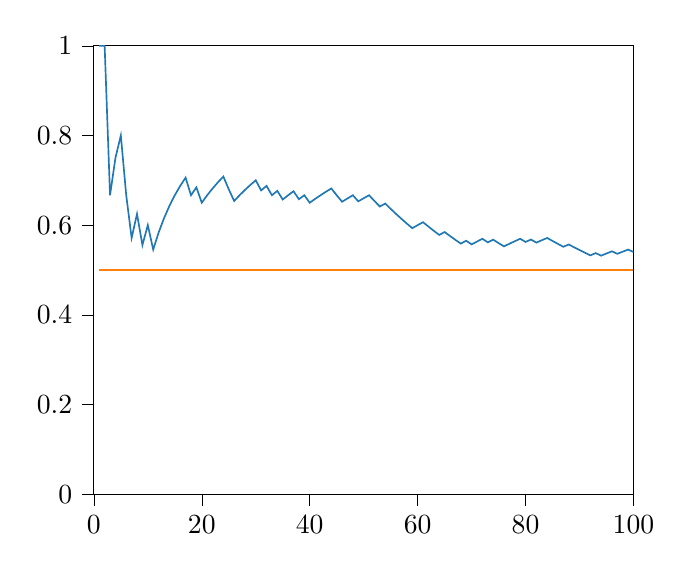
\begin{tikzpicture}
    
            \definecolor{color0}{rgb}{0.12156862745098,0.466666666666667,0.705882352941177}
            \definecolor{color1}{rgb}{1,0.498039215686275,0.0549019607843137}
            
            \begin{axis}[
            tick align=outside,
            tick pos=left,
            x grid style={white!69.0196078431373!black},
            xmin=0, xmax=100,
            xtick style={color=black},
            y grid style={white!69.0196078431373!black},
            ymin=0.0, ymax=1.0,
            ytick style={color=black}
            ]
            \addplot [semithick, color0]
            table {%
            1 1
            2 1
            3 0.666666666666667
            4 0.75
            5 0.8
            6 0.666666666666667
            7 0.571428571428571
            8 0.625
            9 0.555555555555556
            10 0.6
            11 0.545454545454545
            12 0.583333333333333
            13 0.615384615384615
            14 0.642857142857143
            15 0.666666666666667
            16 0.6875
            17 0.705882352941177
            18 0.666666666666667
            19 0.684210526315789
            20 0.65
            21 0.666666666666667
            22 0.681818181818182
            23 0.695652173913043
            24 0.708333333333333
            25 0.68
            26 0.653846153846154
            27 0.666666666666667
            28 0.678571428571429
            29 0.689655172413793
            30 0.7
            31 0.67741935483871
            32 0.6875
            33 0.666666666666667
            34 0.676470588235294
            35 0.657142857142857
            36 0.666666666666667
            37 0.675675675675676
            38 0.657894736842105
            39 0.666666666666667
            40 0.65
            41 0.658536585365854
            42 0.666666666666667
            43 0.674418604651163
            44 0.681818181818182
            45 0.666666666666667
            46 0.652173913043478
            47 0.659574468085106
            48 0.666666666666667
            49 0.653061224489796
            50 0.66
            51 0.666666666666667
            52 0.653846153846154
            53 0.641509433962264
            54 0.648148148148148
            55 0.636363636363636
            56 0.625
            57 0.614035087719298
            58 0.603448275862069
            59 0.593220338983051
            60 0.6
            61 0.60655737704918
            62 0.596774193548387
            63 0.587301587301587
            64 0.578125
            65 0.584615384615385
            66 0.575757575757576
            67 0.567164179104478
            68 0.558823529411765
            69 0.565217391304348
            70 0.557142857142857
            71 0.563380281690141
            72 0.569444444444444
            73 0.561643835616438
            74 0.567567567567568
            75 0.56
            76 0.552631578947368
            77 0.558441558441558
            78 0.564102564102564
            79 0.569620253164557
            80 0.5625
            81 0.567901234567901
            82 0.560975609756098
            83 0.566265060240964
            84 0.571428571428571
            85 0.564705882352941
            86 0.558139534883721
            87 0.551724137931034
            88 0.556818181818182
            89 0.550561797752809
            90 0.544444444444444
            91 0.538461538461538
            92 0.532608695652174
            93 0.537634408602151
            94 0.531914893617021
            95 0.536842105263158
            96 0.541666666666667
            97 0.536082474226804
            98 0.540816326530612
            99 0.545454545454545
            100 0.54
            };
            \addplot [semithick, color1]
            table {%
            1 0.5
            2 0.5
            3 0.5
            4 0.5
            5 0.5
            6 0.5
            7 0.5
            8 0.5
            9 0.5
            10 0.5
            11 0.5
            12 0.5
            13 0.5
            14 0.5
            15 0.5
            16 0.5
            17 0.5
            18 0.5
            19 0.5
            20 0.5
            21 0.5
            22 0.5
            23 0.5
            24 0.5
            25 0.5
            26 0.5
            27 0.5
            28 0.5
            29 0.5
            30 0.5
            31 0.5
            32 0.5
            33 0.5
            34 0.5
            35 0.5
            36 0.5
            37 0.5
            38 0.5
            39 0.5
            40 0.5
            41 0.5
            42 0.5
            43 0.5
            44 0.5
            45 0.5
            46 0.5
            47 0.5
            48 0.5
            49 0.5
            50 0.5
            51 0.5
            52 0.5
            53 0.5
            54 0.5
            55 0.5
            56 0.5
            57 0.5
            58 0.5
            59 0.5
            60 0.5
            61 0.5
            62 0.5
            63 0.5
            64 0.5
            65 0.5
            66 0.5
            67 0.5
            68 0.5
            69 0.5
            70 0.5
            71 0.5
            72 0.5
            73 0.5
            74 0.5
            75 0.5
            76 0.5
            77 0.5
            78 0.5
            79 0.5
            80 0.5
            81 0.5
            82 0.5
            83 0.5
            84 0.5
            85 0.5
            86 0.5
            87 0.5
            88 0.5
            89 0.5
            90 0.5
            91 0.5
            92 0.5
            93 0.5
            94 0.5
            95 0.5
            96 0.5
            97 0.5
            98 0.5
            99 0.5
            100 0.5
            };
            \end{axis}
            
            \end{tikzpicture}
    \end{center}
\noindent
En mathématiques, nous modélisons cette expérience en disant que l'univers des possibles est un
ensemble $\Omega\defeq\ens{P, F}$ formé de deux éléments  et que la probabilité de l'évènement
$A\defeq\ens{P}$ est \nicefrac{1}{2}, ce que l'on note
\[\mathbb{P}(\ens{P})=\frac{1}{2}.\]
Puisque le nombre $n_F$ de fois où on a obtenu face vérifie $n_P+n_F=n$, on en déduit que
la probabilité d'obtenir face est aussi de \nicefrac{1}{2}, ce que l'on note de même
$\mathbb{P}(\ens{F})=1/2$.\\

Considérons maintenant un autre jeu de hasard~: le lancer d'un dé à 6 faces. Dans ce cas,
l'univers des possibles est $\Omega\defeq\intere{1}{6}$. On constate que quel que
soit $\omega\in\Omega$, si on lance le dé $n$ fois et qu'on compte le nombre $n_\omega$ de
fois où on a obtenu $\omega$, la proportion $n_\omega/n$ tend vers $\nicefrac{1}{6}$. On écrira
\[\forall \omega\in\intere{1}{6}\qsep \mathbb{P}(\ens{\omega})=\frac{1}{6}.\]
Si l'on s'intéresse au nombre $n_P$ de fois où on a obtenu un nombre pair, c'est-à-dire au
nombre de fois où on a obtenu 2, 4 ou 6, nous dirons que nous nous intéressons à l'évènement
$A\defeq\ens{2,4,6}$. Bien entendu
\[\frac{n_P}{n}=\frac{n_2+n_4+n_6}{n}=\frac{n_2}{n}+\frac{n_4}{n}+\frac{n_6}{n}
  \tendvers{n}{+\infty} 3\times\frac{1}{6}=\frac{1}{2}.\]
On écrira 
\[\mathbb{P}(\ens{2, 4, 6})=\frac{1}{2}.\]
Nous remarquons que sur ces deux exemples, l'univers $\Omega$ est fini et que, quelle que soit
la partie $A$ de $\Omega$, on a
\[\mathbb{P}(A)=\frac{\card A}{\card \Omega}.\]
Nous dirons que la probabilité $\mathbb{P}$ est uniforme sur $\Omega$.\\

Cependant, les probabilités ne sont pas toujours uniformes. On considère par exemple
l'expérience
qui consiste à avoir 2 enfants. Si on s'intéresse au sexe des enfants, il y a trois
possibilités~: on peut avoir deux filles, deux garçons ou une fille et un garçon. Nous
modélisons cela en disant que l'univers des possibles est $\Omega\defeq\ens{F,G,D}$.
L'expérience montre que la probabilité d'avoir deux filles est de $\nicefrac{1}{4}$,
celle d'avoir deux garçons est de $\nicefrac{1}{4}$ et celle d'avoir une fille et un
garçon est de $\nicefrac{1}{2}$. Nous avons donc un exemple simple où la
probabilité n'est pas uniforme.\\

En 1881, l'astronome
\nom{Simon Newcomb} se rend compte que les livres de tables de logarithmes sont plus
abimés à certaines pages qu'à d'autres. Sa découverte suggère que les personnes
ayant besoin de faire des applications numériques sont plus souvent confrontées à des nombres
commençant par un 1, comme 1491 ou $1.602\times 10^{-19}$, que par un 9, comme $987$ ou $9.81$.
Soixante ans plus tard, \nom{Frank Benford}, après avoir
répertorié un très grand nombre de données, dont les longueurs des fleuves et les populations
des villes, fait le même constat. Ici, l'univers des possibles est $\Omega\defeq\intere{1}{9}$
et \nom{Benford} postule que
\[\forall \omega\in\intere{1}{9}\qsep \mathbb{P}(\ens{\omega})=\log_{10}\p{1+\frac{1}{\omega}}.\]

\begin{center}
% This file was created by tikzplotlib v0.9.8.
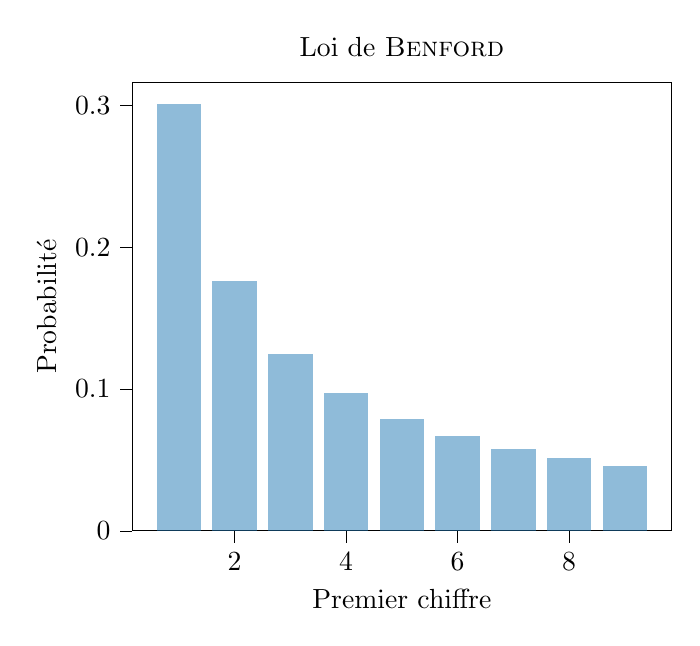
\begin{tikzpicture}

\definecolor{color0}{rgb}{0.12156862745098,0.466666666666667,0.705882352941177}

\begin{axis}[
tick align=outside,
tick pos=left,
title={Loi de \textsc{Benford}},
x grid style={white!69.0196078431373!black},
xlabel={Premier chiffre},
xmin=0.16, xmax=9.84,
xtick style={color=black},
y grid style={white!69.0196078431373!black},
ylabel={Probabilité},
ymin=0, ymax=0.31608149544718,
ytick style={color=black}
]
\draw[draw=none,fill=color0,fill opacity=0.5] (axis cs:0.6,0) rectangle (axis cs:1.4,0.301029995663981);
\draw[draw=none,fill=color0,fill opacity=0.5] (axis cs:1.6,0) rectangle (axis cs:2.4,0.176091259055681);
\draw[draw=none,fill=color0,fill opacity=0.5] (axis cs:2.6,0) rectangle (axis cs:3.4,0.1249387366083);
\draw[draw=none,fill=color0,fill opacity=0.5] (axis cs:3.6,0) rectangle (axis cs:4.4,0.0969100130080564);
\draw[draw=none,fill=color0,fill opacity=0.5] (axis cs:4.6,0) rectangle (axis cs:5.4,0.0791812460476248);
\draw[draw=none,fill=color0,fill opacity=0.5] (axis cs:5.6,0) rectangle (axis cs:6.4,0.0669467896306132);
\draw[draw=none,fill=color0,fill opacity=0.5] (axis cs:6.6,0) rectangle (axis cs:7.4,0.0579919469776867);
\draw[draw=none,fill=color0,fill opacity=0.5] (axis cs:7.6,0) rectangle (axis cs:8.4,0.0511525224473813);
\draw[draw=none,fill=color0,fill opacity=0.5] (axis cs:8.6,0) rectangle (axis cs:9.4,0.0457574905606751);
\end{axis}

\end{tikzpicture}

\end{center}
\noindent
On vérifie que
\begin{eqnarray*}
\sum_{\omega=1}^9 \mathbb{P}(\ens{\omega})
&=& \sum_{\omega=1}^9 \log_{10}\p{1+\frac{1}{\omega}}
= \sum_{\omega=1}^9 \cro{\log_{10}\p{\omega+1}-\log_{10}\p{\omega}}\\
&=& \log_{10}\p{10}-\log_{10}\p{1} = 1
\end{eqnarray*}
comme attendu pour une probabilité.

\subsection{Espace probabilisé}

\begin{definition}
Étant donné une expérience aléatoire, on appelle \emph{univers des possibles} ou simplement
\emph{univers} tout ensemble fini $\Omega$ où chaque élément $\omega\in\Omega$ représente une
\emph{réalisation} de l'expérience.
\end{definition}

\begin{exemples}
\exemple \emph{Série de Pile ou Face}. Soit $n\in\N$. On considère l'expérience aléatoire
  qui consiste à jeter $n$ fois une pièce. Dans ce cas, l'univers des possibles est
  $\Omega\defeq\ens{P,F}^n$, la lettre $P$ représentant le résultat pile et la lettre
  $F$ représentant le résultat face. Par exemple, si $n=3$,
  $\omega\defeq(P,P,F)$ représente la réalisation de l'expérience où les deux premiers
   lancers donnent pile et le dernier lancer donne face.
\exemple \emph{Répartition de $n$ boules discernables dans $p$ urnes discernables}. Soit
  $n,p\in\N$. On considère l'expérience qui consiste à répartir de manière aléatoire $n$
  boules discernables dans $p$ urnes discernables. On choisit de numéroter les boules de
  1 à $n$ et les urnes de $1$ à $p$. L'univers des possibles est donc
  $\Omega_D\defeq\intere{1}{p}^n$ et une réalisation $\omega\in\Omega$ de l'expérience
   est un $n$-uplet $(\omega_1,\ldots,\omega_n)$ où pour tout $i\in\intere{1}{n}$,
  $\omega_i\in\intere{1}{p}$ est le numéro de l'urne dans laquelle on a placé la boule $i$.
\exemple
  \emph{Répartition de $n$ boules indiscernables dans $p$ urnes discernables}. Soit
  $n,p\in\N$. On considère l'expérience qui consiste à répartir de manière aléatoire
  $n$ boules indiscernables dans $p$ urnes discernables. Une réalisation est
  caractérisée par le nombre de boules $x_1,\ldots,x_p\in\N$ que contient chaque urne.
  Comme on sait qu'il y a au total $n$ boules, l'univers des possibles est donc
  \[\Omega_I\defeq\enstq{(x_1,\ldots,x_p)\in\N^p}{x_1+\cdots+x_p=n}.\]
\end{exemples}

\begin{remarqueUnique}
\remarque En première année, l'univers des possibles sera toujours un ensemble fini. Cette
  restriction nous empêchera de modéliser certaines expériences comme jouer à pile ou face
  jusqu'à obtenir pile. La théorie des probabilités sur un univers infini est
  plus délicate. C'est pourquoi vous ne l'aborderez qu'en seconde année.
\end{remarqueUnique}

\begin{definition}
Soit $\Omega$ l'univers des possibles.
\begin{itemize}
\item On appelle \emph{évènement} toute partie de $\Omega$. L'évènement $\Omega$ est appelé
  \emph{évènement certain} et l'évènement $\emptyset$ est appelé \emph{évènement impossible}.
\item On dit que deux évènements $A,B\in\mathcal{P}(\Omega)$ sont
  \emph{disjoints}, ou \emph{incompatibles}, lorsque
  $A\cap B=\emptyset$.
\end{itemize}
\end{definition}

\begin{remarques}
\remarque On dit que les évènements $A_1,\ldots,A_n\in\mathcal{P}(\Omega)$ sont incompatibles
  lorsque
  \[\forall i,j\in\intere{1}{n}\qsep i\neq j\implique A_i\cap A_j=\emptyset.\]
\remarque On dit qu'un évènement $A$ est \emph{élémentaire} lorsqu'il ne contient qu'un résultat
  observable, c'est-à-dire lorsqu'il existe $\omega\in\Omega$ tel que $A=\ens{\omega}$.
\remarque Si $A$ et $B\in\mathcal{P}(\Omega)$ sont des évènements, on appelle
  \begin{itemize}
  \item évènement \og $A$ et $B$ \fg l'évènement $A\cap B$.
  \item évènement \og $A$ ou $B$ \fg l'évènement $A\cup B$.
  \item évènement \og contraire de $A$ \fg l'évènement $\bar{A}=\Omega\setminus A$.
  \end{itemize}
\end{remarques}


\begin{exoUnique}
\exo On considère l'expérience consistant à jeter $n$ fois une pièce.
  Pour tout $k\in\intere{1}{n}$, on considère l'évènement
  $F_k\defeq$ \og Le résultat du $k$-ième lancer est face \fg. Exprimer, en fonction des $F_k$,
  les évènements suivants~:
  \begin{itemize}
  \item $A\defeq$ \og On n'obtient jamais pile au cours des $n$ lancers \fg.
  \item $B\defeq$ \og On obtient pile au moins une fois au cours au cours des $n$ lancers\fg.
  \item $C\defeq$ \og On obtient deux faces consécutifs au cours des $n$ lancers \fg.
  \end{itemize}

\end{exoUnique}

% \begin{exos}
% \exo Soit $A_1,\dots,A_n$ des évènements sur un univers $\Omega$. Exprimer en fonction des
%   $A_i$ les évènements suivants.
%   \begin{itemize}
%   \item $A \defeq$ \og Tous les $A_i$ sont réalisés \fg.
%   \item $B \defeq$ \og L'un des $A_i$ est réalisé \fg.
%   \item $C \defeq$ \og Aucun des $A_i$ n'est réalisé \fg.
%   \item $D \defeq$ \og Au moins l'un des $A_i$ n'est pas réalisé \fg.
%   \item $E \defeq$ \og Un seul des $A_i$ est réalisé \fg.
%   \end{itemize}
% \begin{sol}
% \begin{enumerate}
% \item $\bigcap_{i=1}^n A_i$.
% \item $\bigcup_{i=1}^n A_i$.
% \item $\overline{\bigcup_{i=1}^n A_i}$.
% \item $\bigcup_{i=1}^n \overline{A_i}$.
% \item $\bigcup_{i=1}^n \p{(\cap_{j\neq i}^n \overline{A_j})\cap A_i}$. 
% \end{enumerate}
% \end{sol}
% \exo On tire au hasard deux cartes dans un jeu de 32 cartes
%   (as, roi, dame, valet, 10, 9, 8, 7). On considère les évènements suivants.
%   \begin{itemize}
%   \item $A \defeq$ \og les deux cartes tirées sont rouges \fg
%   \item $B \defeq$ \og les deux cartes tirées sont un valet et un dix \fg
%   \item $C \defeq$ \og les deux cartes tirées sont des personnages \fg
%   \end{itemize}
%   Décrire par des phrases les évènements suivants.
%   \[\bar{A},\quad A \cap B \cap \bar{C},\quad A \cap B \cap C\]
% \begin{sol}
% "Au moins une des cartes n'est pas rouge". "Une carte est un valet rouge et l'autre est un 10 rouge". "C'est l'évènement impossible donc on peut dire n'importe quelle phrase impossible".
% \end{sol}
% \end{exos}
  

\begin{definition}
Soit $\Omega$ l'univers des possibles. On dit que la famille d'évènements
$(A_1,\ldots,A_n)\in\mathcal{P}(\Omega)^n$ forme un \emph{système complet d'évènements}
lorsque c'est une partition de $\Omega$, c'est-à-dire lorsque
\[\Omega = \bigcup_{i=1}^n A_i \qquad\et\qquad \cro{\forall i,j\in\intere{1}{n}\qsep i\neq j\implique
  A_i\cap A_j=\emptyset}.\]
\end{definition}


% \begin{exemples}
% \exemple Dans un casino, il y a $n$ machines à sous. On choisit une machine au hasard et on
%   joue une fois sur cette machine ce qui nous donne soit gagnant, soit perdant.
%   Dans ce cas, l'univers des possibles est
%   $\Omega\defeq\intere{1}{n}\times\ens{g, p}$. Par exemple, un résultat observable de cette
%   expérience est $\omega\defeq(3,g)$; il signifie qu'un a choisi la machine 3 et qu'on a
%   gagné. Pour tout $k\in\intere{1}{n}$, on note $M_k$ l'évènement \og on a choisi la
%   $k$-ième machine \fg. D'autre part, on note $G$ l'évènement \og on a gagné \fg et $P$
%   l'évènement \og on a perdu\fg. Alors $(G,P)$ forme un système complet d'évènements. De
%   même, $(M_1,\ldots,M_n)$ forme un système complet d'évènements
% \end{exemples}

\begin{definition}
On appelle \emph{loi de probabilité}, \emph{mesure de probabilité} ou plus simplement \emph{probabilité} sur un univers $\Omega$
toute application
\[\dspappli{\mathbb{P}}{\mathcal{P}(\Omega)}{\interf{0}{1}}{A}{\mathbb{P}(A)}\]
telle que
\begin{itemize}
\item $\mathbb{P}(\Omega)=1$
\item $\forall A,B\in\mathcal{P}(\Omega)\qsep A\cap B=\emptyset \quad\implique\quad
  \mathbb{P}(A\cup B)=\mathbb{P}(A)+\mathbb{P}(B)$.
\end{itemize}
Le couple $(\Omega,\mathbb{P})$ est appelé \emph{espace probabilisé}.
\end{definition}

\begin{remarqueUnique}
\remarque On dit que deux évènements $A$ et $B$ sont \emph{équiprobables}
  lorsque $\mathbb{P}(A)=\mathbb{P}(B)$.
% \remarque Si $\Omega$ est un ensemble fini non vide, l'application $\mathbb{P}$ définie par
% \[\forall A\in\mathcal{P}(\Omega)\qsep \mathbb{P}(A)=\frac{\card A}{\card \Omega}.\]  
% est une probabilité que nous appelerons \emph{probabilité uniforme}.
\end{remarqueUnique}

\begin{definition}
  Soit $\Omega$ un ensemble fini non vide. On appelle \emph{probabilité uniforme} sur $\Omega$
  l'application $\mathbb{P}:\mathcal{P}(\Omega)\to\interf{0}{1}$ définie par
  \[\forall A\in\mathcal{P}(\Omega)\qsep \mathbb{P}(A)=\frac{\card A}{\card \Omega}.\] 
  \end{definition}
  
  \begin{remarques}
  % \remarque Cherchons à déterminer les probabilités \og naturelles \fg sur les 3 exemples que nous avons
  %   donnés en début de cours.
  \remarque Lorsque $\Omega$ est muni d'une loi uniforme, les calculs de probabilité se ramènent à des
    problèmes de dénombrement.
\remarque Pour deux des trois exemples d'expérience aléatoire que nous avons donné
  en début de cours, la probabilité \og naturelle \fg
  est la probabilité uniforme.
    \begin{itemize}
    \item \emph{Série de Pile ou Face}~: Si on considère l'expérience aléatoire qui consiste à jeter $n$ fois une
      pièce équilibrée, c'est la  probabilité uniforme qui est naturelle sur l'univers $\Omega\defeq\ens{P,F}^n$. Nous montrerons plus tard que cela
      revient à supposer que les
      résultats de chaque lancer ont autant de chance de donner pile que face, et que les lancers sont indépendants.
    \item \emph{Répartition de $n$ boules discernables dans $p$ urnes discernables}~: Si l'on souhaite répartir
      $n$ boules discernables dans $p$ urnes discernables, c'est encore la
      probabilité uniforme qui est naturelle sur $\Omega_D\defeq\intere{1}{p}^n$. Nous verrons que cela revient à supposer que chaque
      boule est placée de manière équiprobable dans les différentes urnes et que ces répartitions sont indépendantes les unes
      des autres.
    % \item \emph{Répartition de $n$ boules indiscernables dans $p$ urnes discernables}~: Enfin, si l'expérience
    %   est de répartir $n$ boules indiscernables dans $p$ urnes discernables, la probabilité naturelle n'est
    %   plus la probabilité uniforme. Pour s'en convaincre, on peut essayer de comprendre ce qui se passe pour
    %   $n=2$ et $p=2$. On considère donc l'expérience qui consiste à placer deux boules indiscernables dans 2 urnes
    %   distinctes. Il y a 3 réalisations possibles de cette expérience~: \og Les deux boules sont dans la première urne \fg,
    %   \og Les deux boules sont dans la seconde urne\fg et \og Il y a une boule dans chaque urne\fg. L'univers des possibles
    %   $\Omega_I$ possède donc 3 éléments. On se convaincra facilement que l'évènement \og Il y a une boule dans
    %   chaque urne \fg a une probabilité naturelle de \nicefrac{1}{2}. En effet, une fois que la première boule est placée,
    %   on a une chance sur deux que la seconde boule soit placée dans la même urne. Les probabilités naturelles
    %   pour cette expérience sont donc respectivement de \nicefrac{1}{4}, \nicefrac{1}{4} et \nicefrac{1}{2}, ce
    %   qui ne dérive pas d'une loi uniforme. Pour traiter ce type de problème, on peut considérer que
    %   les boules sont discernables et travailler sur $\Omega_D$ muni de la probabilité uniforme.
    \end{itemize}
  \end{remarques}

Dans la suite de ce cours, $(\Omega,\mathbb{P})$ désignera un espace probabilisé.

\begin{proposition}
\begin{eqnarray*}
\mathbb{P}(\emptyset)=0,& &\mathbb{P}(\Omega)=1,\\
\forall A\in\mathcal{P}(\Omega),& &\mathbb{P}(\bar{A})=1-\mathbb{P}(A),\\
\forall A,B\in\mathcal{P}(\Omega),& &\mathbb{P}(A\cup B)=\mathbb{P}(A)+\mathbb{P}(B)-\mathbb{P}(A\cap B).
\end{eqnarray*}
\end{proposition}

\begin{proposition}
Une probabilité est une fonction \emph{croissante}. Autrement dit
\[\forall A,B\in\mathcal{P}(\Omega)\qsep A\subset B \quad\implique\quad \mathbb{P}(A)\leq\mathbb{P}(B).\]
\end{proposition}

\begin{proposition}
Soit $(A_1,\ldots,A_n)\in\mathcal{P}(\Omega)^n$ une famille d'évènements incompatibles.
Alors
\[\mathbb{P}\p{\bigcup_{i=1}^n A_i}=\sum_{i=1}^n \mathbb{P}(A_i).\]
\end{proposition}

\begin{remarques}
\remarque Si $A_1,\ldots,A_n$ est une famille d'évènements incompatibles, la réunion des $A_i$ est parfois
  notée
  \[\bigsqcup_{i=1}^n A_i.\]
\remarque Si $A_1,\ldots,A_n$ sont quelconques, on a seulement
  \[\mathbb{P}\p{\bigcup_{i=1}^n A_i}\leq\sum_{i=1}^n \mathbb{P}(A_i).\]
  On dit que $\mathbb{P}$ est \emph{sous-additive}. 
\end{remarques}

\begin{exos}
  \exo Une urne contient 20 boules, numérotées de 1 à 20~: 5 boules sont blanches,
  5 sont rouges et 10 sont noires.
  On tire successivement 3 boules, avec remise à chaque tirage.
  Si on munit $\Omega$ de la probabilité uniforme,
  calculer la probabilité que
    le tirage soit~:
    \begin{itemize}
  \item unicolore.
  \item tricolore.
  \item bicolore.
    \end{itemize}
  % \question On tire 3 boules simultanément. Reprendre les questions précédentes.
  % \end{questions}
  \begin{sol}
  \begin{questions}
  \question $\Card\Omega=20^3=8000$~: ce sont des triplets de $\intere{1}{20}$. La loi de probabilité est uniforme.
    \begin{itemize}
    \item $\Card A=10\times 5\time 5\times 3!$. On trouve une probabilité de $3/16$.
    \item $\Card B=375+375+1500+750+1500+750$. On troube une proba de $21/32$.
    \item $\Card C=125+!25+1000$. On trouve une proba de $5/32$.
    \end{itemize}
  \question $\Card\Omega=\binom{20}{3}=1440$.
    \begin{itemize}
    \item $250$, puis $25/114$.
<    \item $25/38$.
    \item $7/57$.
    \end{itemize}
  \end{questions}
  \end{sol}
  \exo Une urne contient 8 boules, numérotées de 1 à 8~: 3 boules sont blanches et
    5 sont noires. On en tire simultanément 4 boules.
    Si on munit $\Omega$ de la probabilité uniforme, avec quelle probabilité
    n'a-t-on tiré que des boules noires~?
    \begin{sol}
    On trouve (4 parmi 5)/(4 parmi 8) et donc \nicefrac{1}{14}.
    \end{sol}
\end{exos}

\begin{proposition}[nom={Formule du crible}]
Soit $(A_1,\ldots,A_n)\in\mathcal{P}(\Omega)^n$ une famille d'évènements. Alors
  \[\mathbb{P}\p{\bigcup_{i=1}^n A_i}=\sum_{k=1}^n (-1)^{k+1}
    \sum_{1\leq i_1<\cdots<i_k\leq n}
    \mathbb{P}\p{A_{i_1}\cap\cdots\cap A_{i_k}}.\]
\end{proposition}

\begin{remarqueUnique}
\remarque   Par exemple, pour $n=3$, la formule du crible s'écrit
\[\mathbb{P}\p{A_1\cup A_2\cup A_3}=\mathbb{P}(A_1)+\mathbb{P}(A_2)+\mathbb{P}(A_3) - \cro{\mathbb{P}(A_2\cap A_3)+\mathbb{P}(A_1\cap A_3)+\mathbb{P}(A_1\cap A_2)}+\mathbb{P}(A_1\cap A_2\cap A_3).\]
\end{remarqueUnique}


\begin{definition}
\begin{itemize}
\item On appelle \emph{distribution de probabilité} sur
  $\Omega$ toute famille $(p_{\omega})_{\omega\in\Omega}$ de réels positifs telle que
  \[\sum_{\omega\in\Omega} p_{\omega}=1.\]
\item Si $\mathbb{P}$ est une probabilité sur $\Omega$, on appelle \emph{distribution de
  probabilité} de $\mathbb{P}$ la famille $(p_{\omega})_{\omega\in\Omega}$ définie par
  \[\forall \omega\in\Omega\qsep p_{\omega}\defeq \mathbb{P}(\ens{\omega}).\]
  C'est une distribution de probabilité sur $\Omega$.
\end{itemize}
\end{definition}

% \begin{remarqueUnique}
% \remarque Si $(p_\omega)_{\omega\in\Omega}$ est une distribution de probabilité sur $\Omega$, on appelle support
%   de $p$ l'ensemble $\enstq{\omega\in\Omega}{p_{\omega}>0}$.
%   Par extension, le support d'une probabilité $\mathbb{P}$ est le support de sa distribution de probabilité.
%   Autrement dit
%   \[{\rm Supp}(\mathbb{P})\defeq\enstq{\omega\in\Omega}{\mathbb{P}(\ens{\omega})>0}.\]
%   % On s'intéressera le plus souvent à des espaces probabilisés $(\Omega,\mathbb{P})$
%   % pour lesquels ${\rm Supp}(\mathbb{P})=\Omega$.
% \end{remarqueUnique}
\begin{remarqueUnique}
  \remarque Si $\mathbb{P}$ désigne la probabilité uniforme sur l'univers $\Omega$ de cardinal $n$, alors
quel que soit $\omega\in\Omega$, $p_\omega=1/n$.
\end{remarqueUnique}

\begin{exoUnique}
\exo Sur l'univers $\Omega\defeq\intere{0}{n}$, on définit la famille $(p_k)_{0\leq k\leq n}$ par
  \[\forall k\in\intere{0}{n}\qsep p_k\defeq\alpha\binom{n}{k}\]
  où $\alpha\in\R$. Déterminer $\alpha$ pour que $(p_k)_{0\leq k\leq n}$ soit une distribution de probabilité. 
\end{exoUnique}


\begin{proposition}
Soit $(\Omega,\mathbb{P})$ un espace probabilisé et $(p_\omega)_{\omega\in\Omega}$ la distribution de probabilité de $\mathbb{P}$. Alors
\[\forall A\in\mathcal{P}(\Omega)\qsep \mathbb{P}(A)=\sum_{\omega\in A} p_{\omega}.\]
\end{proposition}

\begin{remarques}
\remarque Une probabilité est donc entièrement déterminée par sa distribution de probabilité.
% \remarque 
  % Un évènement $A$ est presque sûr si et seulement si ${\rm Supp}(\mathbb{P})\subset A$.
% \remarque En particulier, deux probabilités $\mathbb{P}_1$ et $\mathbb{P}_2$, définies sur un même univers
%   $\Omega$, sont égales si et seulement si
%   \[\forall \omega\in\Omega\qsep \mathbb{P}_1(\ens{\omega})=\mathbb{P}_2(\ens{\omega}).\]
\remarque Une probabilité est donc uniforme si et seulement si tous les évènements élémentaires sont équiprobables.
Une erreur très classique en probabilités est de croire que la mesure de probabilité \og naturelle \fg
sur un univers est toujours la probabilité uniforme. Ce n'est pas toujours le cas. Cependant, lorsque ça l'est,
un argument de symétrie permet souvent de s'en convaincre.
Par exemple, si on lance un dé à 6 faces, les symétries du dé font que les valeurs obtenues sont
équiprobables. La mesure de probabilité \og naturelle \fg sur $\Omega\defeq\intere{1}{6}$ est donc la probabilité
uniforme.
\end{remarques}

\begin{exoUnique}
\exo On lance un dé pipé à 6 faces qui donne \og 1 \fg avec la probabilité \nicefrac{1}{4} et les
  autres faces avec une même probabilité $p$. Quelle est la probabilité d'obtenir un nombre impair~?
  \begin{sol}
  On trouve $p=3/20$, et $\mathbb{P}(Impair)=11/20$.
  \end{sol}
\end{exoUnique}

\begin{proposition}
Soit $(p_\omega)_{\omega\in\Omega}$ une distribution de probabilité sur l'univers $\Omega$. Alors il existe une
unique probabilité $\mathbb{P}$ sur $\Omega$ telle que
\[\forall \omega\in\Omega\qsep \mathbb{P}(\ens{\omega})=p_{\omega}.\]
\end{proposition}

% \begin{remarques}
% \remarque On considère l'expérience aléatoire qui consiste à lancer une pièce. L'univers
%   des possibles est $\Omega\defeq\ens{P,F}$, la lettre $P$ représentant le résultat pile,
%   et la lettre $F$ représentant le résultat face. Si la pièce est équilibrée, l'expérience
%   montre que la probabilité d'obtenir une pile est de \nicefrac{1}{2} et la probabilité
%   d'obtenir un face est de \nicefrac{1}{2}. C'est bien la probabilité
%   uniforme sur $\Omega$. 
% \remarque On considère l'expérience aléatoire qui consiste à lancer un dé à 6 faces.
%   L'univers des possibles est $\Omega\defeq\intere{1}{6}$. Si le dé n'est pas pipé,
%   l'expérience montre que quel que soit $\omega\in\intere{1}{6}$, la probabilité d'obtenir
%   $\omega$ est de \nicefrac{1}{6}. La probabilité naturelle sur $\Omega$ est donc la
%   probabilité uniforme.
% \remarque Soit $n\in\N$. On considère l'expérience aléatoire qui consiste à lancer $n$
%   fois une pièce. L'univers des possibles est donc $\Omega\defeq\ens{P,F}^n$.
%   En supposant que la probabilité d'obtenir un pile à chaque lancer est de \nicefrac{1}{2} et
%   que les lancers sont mutuellements indépendants, nous démontrerons plus tard que tous les
%   résultats sont équiprobables. La probabilité naturelle sur $\Omega$ est donc la probabilité
%   uniforme.
% \remarque Soit $n,p\in\N$. On considère l'expérience aléatoire qui consiste à placer $n$
%   boules discernables dans $p$ urnes discernables. En numérotant les boules de 1 à $n$ et
%   les urnes de 1 à $p$, l'univers des possibles est
%   $\Omega\defeq\mathcal{F}(\intere{1}{n},\intere{1}{p})$, un résultat observable étant une
%   application $\omega\in\Omega$ qui a une boule $i\in\intere{1}{n}$ associe l'urne $\omega(i)\in\intere{1}{p}$
%   dans laquelle elle a été placée. En supposant que les boules sont placées les unes
%   après les autres avec une probabilité uniforme sur toutes les urnes et qu'elle sont placées
%   de manière indépendante, nous démontrerons plus tard que tous les résultats sont
%   équiprobables. La probabilité naturelle sur $\Omega$ est donc la probabilité
%   uniforme.
% \end{remarques}

% \begin{proposition}
% Soit $\Omega=\ens{\omega_1,\ldots,\omega_n}$ un ensemble fini de cardinal $n$ et
% $p_1,\ldots,p_n\in\RP$ tels que $p_1+\cdots+p_n=1$. Alors il existe une unique
% mesure de probabiblité $\mathbb{P}$ sur $\Omega$ telle que
% \[\forall i\in\intere{1}{n}\qsep \mathbb{P}(\ens{\omega_i})=p_i.\]
% \end{proposition}



% \begin{definition}
% Soit $(\Omega,\mathbb{P})$ un espace probabilisé, $\Omega'$ un ensemble fini et
% $f:\Omega\to\Omega'$. Alors l'application
% \[\dspappli{\mathbb{P}_f}{\mathcal{P}(\Omega')}{\interf{0}{1}}{A}{\mathbb{P}\p{f^{-1}(A)}}\]
% est une probabilité sur $\Omega'$, appelée \emph{mesure image} de $\mathbb{P}$ par $f$.
% \end{definition}



% Ici, il faut parler de boules discernables et indiscernables.

% \begin{remarqueUnique}
% \remarque Soit $n,p\in\N$. On considère l'expérience aléatoire qui consiste à placer $n$
%   boules indiscernables dans $p$ urnes discernables. On note $\Omega$ l'univers des
%   possibles. Pour définir une probabilité
%   naturelle sur $\Omega$, il est bon de commencer par imaginer que les boules sont
%   discernables. Cela nous conduit à considérer l'univers $\Omega_1\defeq\mathcal{F}(\intere{1}{n},\intere{1}{p})$
%   muni de la probabilité uniforme $\mathbb{P}_1$. 
%   %  En numérotant les boules de 1 à $n$ et
%   % les urnes de 1 à $p$, l'univers des possibles est
%   % $\Omega\defeq\mathcal{F}(\intere{1}{n},\intere{1}{p})$, un résultat observable étant une
%   % application $\omega\in\Omega$ qui a une boule $i\in\intere{1}{n}$ associe l'urne $\omega(i)\in\intere{1}{p}$
%   % dans laquelle elle a été placée. En supposant que les boules sont placées les unes
%   % après les autres avec une probabilité uniforme sur toutes les urnes et qu'elle sont placées
%   % de manière indépendante, nous démontrerons plus tard que tous les résultats sont
%   % équiprobables. La probabilité naturelle sur $\Omega$ est donc la probabilité
%   % uniforme.
% \end{remarqueUnique}

\subsection{Variable aléatoire}

\begin{definition}
Soit $(\Omega,\mathbb{P})$ un espace probabilisé. On appelle \emph{variable aléatoire}
à valeurs dans $E$ toute application $X:\Omega\to E$.
\end{definition}

\begin{remarqueUnique}
\remarque On dit qu'une variable aléatoire $X:\Omega\to E$ est réelle lorsque $E$ est une
  partie de $\R$.
% \remarque Puisque $\Omega$ est fini, $X(\Omega)$ est fini. Si $E'$ est une partie finie de $E$
%   telle que $X(\Omega)\subset E'$, on se permettra de confondre $X$ et sa corestriction
%   à $E'$. On pourra donc se ramener au cas où $E$ est fini.
\end{remarqueUnique}

\begin{definition}
Soit $X:\Omega\to E$ une variable aléatoire. Alors, pour toute partie $A$ de $E$, on définit
l'évènement
\[(X\in A)\defeq\enstq{\omega\in\Omega}{X(\omega)\in A}.\] 
\end{definition}

\begin{remarques}
\remarque Si $x\in E$, l'évènement $\enstq{\omega\in\Omega}{X(\omega)=x}$ est noté
  $(X=x)$.
\remarque Si $X$ est une variable aléatoire réelle et $a,b\in\R$, l'évènement
  $\enstq{\omega\in\Omega}{a\leq X(\omega)\leq b}$ est noté $(a\leq X\leq b)$. 
\remarque L'évènement $(X\in A)$ est aussi noté $\ens{X\in A}$ ou $[X\in A]$. La probabilité
  d'un tel évènement est notée $\mathbb{P}(X\in A)$.
\end{remarques}

\begin{proposition}
Soit $X:\Omega\to E$ une variable aléatoire et $A,B\in\mathcal{P}(E)$. Alors
\[(X\in A\cap B)=(X\in A)\cap(X\in B), \qquad (X\in A\cup B)=(X\in A)\cup(X\in B),\]
\[(X\in \bar{A})=\overline{(X\in A)}.\]
\end{proposition}

\begin{exoUnique}
\exo Soit $X:\Omega\to\Z$ une variable aléatoire à valeurs entières. Montrer que
  \[\forall n\in\Z\qsep \mathbb{P}(X=n)=\mathbb{P}(X\leq n) - \mathbb{P}(X\leq n-1).\]
% \exo Soit $X$ une variable aléatoire réelle. Montrer que
%   $\mathbb{P}(X\leq 1)\leq \mathbb{P}(\abs{X-2}\geq 1)$.
% \exo On joue $n\in\Ns$ fois à pile ou face avec une pièce équilibrée. On compte le nombre
%   de lancers nécessaires $X$ pour obtenir pile pour la première fois. Si on obtient que des
%   faces, on pose $X=n+1$.
%   \begin{questions}
%   \question Modéliser l'expérience en précisant l'univers des possibles $\Omega$ et donner
%     une probabilité naturelle sur $\Omega$.
%   \question Pour tout $k\in\intere{0}{n}$, calculer $\mathbb{P}(X>k)$.
%   \question En déduire $\mathbb{P}(X=k)$ pour tout $k\in\intere{1}{n+1}$.
%   \end{questions}
\end{exoUnique}


\begin{definition}
Soit $X:\Omega\to E$ une variable aléatoire. Alors l'application
\[\dspappli{\mathbb{P}_X}{\mathcal{P}(X(\Omega))}{\interf{0}{1}}{A}{\mathbb{P}\p{X\in A}}\]
est une probabilité sur $X(\Omega)$, appelée \emph{loi} de $X$.
\end{definition}

\begin{remarques}
\remarque La loi de $X$ est entièrement déterminée par
  sa distribution de probabilité $(\mathbb{P}(X=x))_{x\in X(\Omega)}$.
\remarque Si $x\in E$ n'appartient pas à $X(\Omega)$, alors $\mathbb{P}(X=x)=0$.
\remarque 
  En pratique, lorsqu'il nous sera demandé de déterminer la loi d'une variable aléatoire
  $X:\Omega\to E$, on commencera par déterminer un ensemble fini $E'$ tel que $X(\Omega)\subset E'$
  puis on calculera $\mathbb{P}(X=x)$ pour tout $x\in E'$.
\remarque Si $(\Omega_1,\mathbb{P}_1)$ est un espace probabilisé, $\Omega_2$ est un ensemble fini et
  $F$ est une application de $\Omega_1$ dans $\Omega_2$, alors
  \[\dspappli{\mathbb{P}_2}{\mathcal{P}(\Omega_2)}{\interf{0}{1}}{A}{\mathbb{P}_1\p{F\in A}}\] 
  est une probabilité sur $\Omega_2$, appelée \emph{mesure image} de $\mathbb{P}_1$ par $F$.
\remarque
  En reprenant les notations utilisées dans les exemples de répartition de $n$ boules  
  discernables/indiscernables
  dans $p$ urnes discernables donnés plus haut, 
  on considère la fonction d'oubli $F:\Omega_D\to\Omega_I$. À une répartition de boules numérotées et donc discernables, elle associe
  la répartition
  des boules indiscernables, où on a effacé le numéro des boules. Autrement dit, si
  $\omega\defeq(\omega_1,\ldots,\omega_n)\in\Omega_D$, alors
  $F(\omega)=(x_1,\ldots,x_p)\in\Omega_I$ où
  \[\forall j\in\intere{1}{p}\qsep x_j=\card\enstq{i\in\intere{1}{n}}{\omega_i=j}.\]
La mesure de probabilité naturelle sur $\Omega_I$ est la mesure image par $F$ de la probabilité uniforme sur
  $\Omega_D$.
\end{remarques}

% \begin{remarques}
% % \remarque Le \emph{support de la variable aléatoire $X$} est défini comme étant le support
% %   de $\mathbb{P}_X$. Autrement dit
% %   \[{\rm Supp}(X)\defeq\enstq{x\in E}{\mathbb{P}(X=x)>0}.\]
% %   Remarquons que ${\rm Supp}(X)\subset X(\Omega)$, l'inclusion pouvant être stricte.
% \remarque Si l'on souhaite définir la loi d'une variable aléatoire $X:\Omega\to E$ à
%   valeurs dans un ensemble infini $E$, il suffit de considérer la corestriction
%   de $X$ à l'ensemble fini $E'\defeq X(\Omega)$. Étant donné que la détermination
%   exacte de $X(\Omega)$ nécessite parfois de traiter de nombreux
%   cas particuliers, nous nous contenterons de corestreindre $X$ à un ensemble fini $E'$ tel
%   que $X(\Omega)\subset E'$. Par exemple, si
%   $A\in\mathcal{P}(\Omega)$ et $X:\Omega\to\R$ est la fonction indicatrice
%   \[\dspappli{X}{\Omega}{\R}{\omega}{
%   \begin{cases}
%   1 & \text{si $\omega\in A$}\\
%   0 & \text{si $\omega\not\in A$.}
%   \end{cases}}\]
%   Alors $X(\Omega)\subset\ens{0,1}$. Cette inclusion est une égalité, sauf dans les cas
%   particuliers où $A=\emptyset$ et $A=\Omega$, pour lesquels $X(\Omega)$ est
%   respectivement égal à $\ens{0}$ et à $\ens{1}$. Pour une telle variable aléatoire,
%   on choisit $E'\defeq\ens{0,1}$. La distribution de probabilité $(p_0,p_1)$ de
%   $\mathbb{P}_X$ est alors donnée par
%   \[p_0=1-\mathbb{P}(A) \et p_1=\mathbb{P}(A).\]
%   Le plus souvent, on confondra $E'$ et $X(\Omega)$ et on écrira abusivement
%   $X(\Omega)=\ens{0,1}$.

% \end{remarques}

\begin{exoUnique}
\exo On lance successivement deux dés à 6 faces. On modélise cette expérience en choisissant $\Omega\defeq\intere{1}{6}^2$
  muni de la probabilité uniforme. On note $A_1:\Omega\to\N$ le résultat du premier dé et
  $A_2:\Omega\to\N$ le résultat du second dé. Déterminer les lois de $A_1$, $A_2$ ainsi que
  la loi de la variable aléatoire $A_1+A_2:\Omega\to\N$ donnant la somme des deux nombres
  obtenus.
\end{exoUnique}


% \begin{remarqueUnique}
  % Pour s'en convaincre, on considère l'expérience aléatoire qui consiste à jouer 2
  % fois à pile ou face. On modèlise cette expérience en posant $\Omega\defeq\ens{P,F}^2$ que
  % l'on munit de la probabilité uniforme. Soit $X_1:\Omega\to\ens{P,F}$ et
  % $X_2:\Omega\to\ens{P,F}$ les variables aléatoires donnant respectivement les résultats des
  % premiers et seconds lancers.  Alors $X_1$ et $X_2$ suivent la même loi. Pourtant, elles ne
  % sont pas égales.
% \end{remarqueUnique}

  
\begin{proposition}
Soit $X:\Omega\to E$ une variable aléatoire. Alors, pour toute partie $A$ de $E$
  \[\mathbb{P}(X\in A)=\sum_{x\in A} \mathbb{P}(X=x)\]
\end{proposition}

\begin{remarqueUnique}
\remarque Étant donné que $\mathbb{P}(X=x)$ est nul pour tout $x$ en dehors de l'ensemble
  fini $X(\Omega)$, cette somme est bien définie puisqu'elle ne comporte qu'un nombre fini
  de termes non nuls.
\end{remarqueUnique}


\begin{definition}
On dit que deux variables aléatoires $X,Y:\Omega\to E$ suivent la même
loi lorsque
\[\forall A\in\mathcal{P}(E)\qsep \mathbb{P}(X\in A)=\mathbb{P}(Y\in A).\]
Si tel est le cas, on écrit $X\sim Y$.
\end{definition}

\begin{remarques}
\remarque En pratique, pour montrer que $X$ et $Y$ suivent la même loi, il suffit de déterminer
  un ensemble fini $E'$ tel que $X(\Omega)\subset E'$ et $Y(\Omega)\subset E'$, puis de
  montrer que
  \[\forall a\in E'\qsep \mathbb{P}(X=a)=\mathbb{P}(Y=a).\]
\remarque Deux variables aléatoires qui suivent la même loi sont rarement égales.
  Par exemple, si $A$ est un évènement de probabilité \nicefrac{1}{2}, les variables
  aléatoires $\mathds{1}_A$ et $\mathds{1}_{\bar{A}}$ suivent la même loi sans être
  égales.
\end{remarques}

\begin{proposition}
Si $X:\Omega\to E$ une variable aléatoire, $X(\Omega)$ est un ensemble fini que l'on
note $\ens{x_1,\ldots,x_n}$. Alors, la famille des $(X=x_i)$ pour $i\in\intere{1}{n}$ forme
un système complet d'évènements.
\end{proposition}

\begin{remarques}
\remarque On utilisera souvent ce système complet d'évènements dans la formule des
  probabilités totales.
\remarque Cette proposition reste vraie si on remplace $X(\Omega)$ par une partie finie
  $E'$ de $E$ telle que $X(\Omega)\subset E'$.
\end{remarques}


\begin{definition}
Soit $X:\Omega\to E$ une variable aléatoire et $f:E\to F$. On note $f(X)$ la variable
aléatoire $f\circ X:\Omega\to F$.
\end{definition}

% \begin{proposition}

% \end{proposition}

% \begin{remarqueUnique}
% \remarque
 
% cette formule restant vraie si l'on remplace $X(\Omega)$ par une partie finie $E'$ de $E$
% telle que $X(\Omega)\subset E'$.
% \end{remarqueUnique}

\begin{remarqueUnique}
\remarque Soit $X:\Omega\to E$ une variable aléatoire et $f:E\to F$. Alors, pour tout
$y\in F$
\[\mathbb{P}(f(X)=y)=\sum_{x\in f^{-1}(\ens{y})} \mathbb{P}(X=x)\] 
  % \remarque Étant donné que $\mathbb{P}(X=x)$ est nul pour tout $x$ en dehors de l'ensemble
  %   fini $X(\Omega)$, cette somme est bien définie puisqu'elle ne comporte qu'un nombre fini
  %   de termes non nuls.
  \end{remarqueUnique}

\begin{proposition}
Soit $X,Y:\Omega\to E$ deux variables aléatoires et $f:E\to F$. Si $X\sim Y$, alors
$f(X)\sim f(Y)$.
\end{proposition}



\subsection{Lois usuelles}

% \begin{definition}[nom={Variable aléatoire constante}]
% On dit qu'une variable aléatoire $X:\Omega\to E$ est \emph{constante} lorsqu'il existe $a\in E$ tel
% que
% \[\mathbb{P}(X=a)=1.\]
% \end{definition}

% \begin{remarques}
% % \remarque Si $X:\Omega\to E$ est une variable aléatoire constante, il existe un unique
% %   $a\in E$ tel que $\mathbb{P}(X=a)=1$; on dit que $X$ est une variable aléatoire
% %   constante égale à $a$.
% % \remarque Une variable aléatoire $X:\Omega\to E$ est constante égale à $a\in E$, si et
% %   seulement si il existe un évènement presque sûr $A$ tel que
% %   \[\forall\omega\in A\qsep X(\omega)=a.\]
% \remarque Si $X:\Omega\to E$ est constante égale à $a$, alors
%   \[\forall x\in E\qsep \mathbb{P}(X=x)=
%   \begin{cases}
%   1 & \text{si $x=a$,}\\
%   0 & \text{sinon.}
%   \end{cases}\]
%   En particulier, ${\rm Supp}(\mathbb{P}_X)=\ens{a}$. On écrira parfois abusivement $X(\Omega)=\ens{a}$.
% \remarque Une variable aléatoire $X:\Omega\to E$ est constante si et seulement si il existe $a\in E$ et
%   un évènement presque sûr $A$ tel que
%   \[\forall \omega\in A\qsep X(\omega)=a.\]
% \end{remarques}


\begin{definition}[nom={Loi uniforme}]
Soit $A$ un ensemble fini non vide. On dit qu'une variable aléatoire $X$ à valeurs dans $A$
suit une \emph{loi uniforme} sur $A$ lorsque
\[\forall a\in A\qsep \mathbb{P}(X=a)=\frac{1}{\card A}.\]
Si tel est le cas, on note $X\sim\mathcal{U}(A)$.
\end{definition}

\begin{remarqueUnique}
\remarque Si $X$ suit une loi uniforme sur $A$, alors $X(\Omega)=A$.
\end{remarqueUnique}
% \begin{remarqueUnique}
% \remarque $X:\Omega\to A$ suit une loi uniforme sur $A$
% %   si et seulement si $\mathbb{P}_X$ est la probabilité uniforme sur $A$.
% \remarque Si $X:\Omega\to E$ suit une loi uniforme sur $A$, alors
%   \[\forall x\in E\qsep \mathbb{P}(X=x)=
%   \begin{cases}
%   \frac{1}{\card A} & \text{si $x\in A$,}\\
%   0 & \text{sinon.}
%   \end{cases}\]
%   En particulier, ${\rm Supp}(\mathbb{P}_X)=A$. On écrira parfois abusivement $X(\Omega)=A$.
% \end{remarqueUnique}
% \vspace{1ex}
\begin{exoUnique}
\exo Soit $X$ une variable aléatoire suivant une loi uniforme sur $\intere{-2}{2}$. Déterminer la loi
  de $X^2+1$.
\end{exoUnique}


\begin{definition}[nom={Loi de \nom{Bernoulli}}]
Soit $p\in[0,1]$. On dit qu'une variable aléatoire $X$ à valeurs dans $\ens{0,1}$ suit la \emph{loi de
\nom{Bernoulli}} de paramètre $p$ lorsque
\[\mathbb{P}(X=1)=p.\]
Si tel est le cas, $\mathbb{P}(X=0)=1-p$ et on note $X\sim\mathcal{B}(p)$.
\end{definition}

\begin{remarques}
\remarque Si $p\in[0,1]$, il est courant de poser $q\defeq 1-p\in[0,1]$.
% \remarque On a ${\rm Supp}(\mathbb{P}_X)\subset\ens{0,1}$, cette inclusion étant une
%   égalité si et seulement si $p\in]0,1[$.
%   On écrira parfois abusivement $X(\Omega)=\ens{0,1}$.
\remarque Si $X$ suit une loi de Bernoulli de paramètre $p\in]0,1[$, alors $X(\Omega)=\ens{0,1}$.
\remarque Toute variable aléatoire $X$ à valeurs dans $\ens{0,1}$ suit une loi de \nom{Bernoulli}
  de paramètre $p\defeq\mathbb{P}(X=1)$. En particulier, si $A\in\mathcal{P}(\Omega)$ est un évènement,
  alors $\mathds{1}_A$ est une variable aléatoire qui suit une
  loi de \nom{Bernoulli} de paramètre $p\defeq\mathbb{P}(A)$.
% \remarque Une loi de $\nom{Bernoulli}$ est constante si et seulement si $p=0$ ou $p=1$.
\remarque On dit qu'une variable aléatoire $Y$ à valeurs dans $\ens{-1,1}$ suit une loi de
  \nom{Rademacher} lorsque
  \[\mathbb{P}(Y=-1)=\frac{1}{2} \quad\et\quad \mathbb{P}(Y=1)=\frac{1}{2}.\]
  % Une variable aléatoire $Y$ suit une loi de \nom{Rademacher} si et seulement si il existe
  % une variable aléatoire $X$ suivant une loi de \nom{Bernoulli} de paramètre \nicefrac{1}{2}
  % telle que $Y=-1+2X$.
\end{remarques}

\begin{exempleUnique}
\exemple On considère l'expérience aléatoire d'un tir de penalty dans un match de foot. 
  La variable aléatoire $X:\Omega\to\ens{0,1}$ décrit le résultat de ce tir~: 1 si le
  penalty est réussi et 0 si le penalty est manqué. $X$ suit donc une loi de
  \nom{Bernoulli} dont le paramètre $p$ est estimé, selon les joueurs, entre $70\%$ et $90\%$.
\end{exempleUnique}

\begin{definition}[nom={Loi binomiale}]
Soit $n\in\N$ et $p\in[0,1]$. On dit qu'une variable aléatoire $X$ à valeurs dans $\intere{0}{n}$
suit la \emph{loi binomiale} de paramètre $(n,p)$ lorsque
\[\forall k\in\intere{0}{n}\qsep \mathbb{P}(X=k)=\binom{n}{k}p^k(1-p)^{n-k}.\]
Si tel est le cas, on note $X\sim\mathcal{B}(n,p)$. 
\end{definition}

\begin{remarques}
\remarque La loi binomiale $\mathcal{B}(1,p)$ n'est autre
  que la loi de \nom{Bernoulli} de paramètre $p$.
% \remarque On a ${\rm Supp}(\mathbb{P}_X)\subset\intere{0}{n}$, cette inclusion étant une
%   égalité si et seulement si $p\in ]0,1[$.
%   On écrira parfois abusivement $X(\Omega)=\intere{0}{n}$.
\remarque Si $X$ suit une loi binomiale de paramètre $(n,p)$ où $p\in]0,1[$, alors $X(\Omega)=\intere{0}{n}$.
\end{remarques}


% from scipy.special import binom
% import matplotlib.pyplot as plt
% import tikzplotlib as tikz
% n = 10
% p = 0.2
% r = [binom(n, k) * p**k * (1-p)**(n-k) for k in range(n)]
% plt.bar(range(n), r, alpha=0.5)
% tikz.save('/Users/fayard/Desktop/binomial-10.tex')

\begin{center}
% This file was created by tikzplotlib v0.9.8.
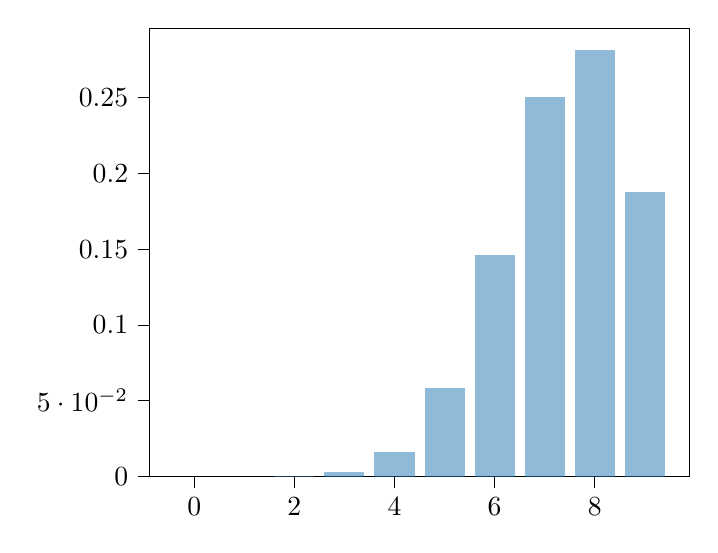
\begin{tikzpicture}

\definecolor{color0}{rgb}{0.12156862745098,0.466666666666667,0.705882352941177}

\begin{axis}[
tick align=outside,
tick pos=left,
x grid style={white!69.0196078431373!black},
xmin=-0.89, xmax=9.89,
xtick style={color=black},
y grid style={white!69.0196078431373!black},
ymin=0, ymax=0.295645952224731,
ytick style={color=black}
]
\draw[draw=none,fill=color0,fill opacity=0.5] (axis cs:-0.4,0) rectangle (axis cs:0.4,9.5367431640625e-07);
\draw[draw=none,fill=color0,fill opacity=0.5] (axis cs:0.6,0) rectangle (axis cs:1.4,2.86102294921875e-05);
\draw[draw=none,fill=color0,fill opacity=0.5] (axis cs:1.6,0) rectangle (axis cs:2.4,0.000386238098144531);
\draw[draw=none,fill=color0,fill opacity=0.5] (axis cs:2.6,0) rectangle (axis cs:3.4,0.00308990478515625);
\draw[draw=none,fill=color0,fill opacity=0.5] (axis cs:3.6,0) rectangle (axis cs:4.4,0.0162220001220703);
\draw[draw=none,fill=color0,fill opacity=0.5] (axis cs:4.6,0) rectangle (axis cs:5.4,0.0583992004394531);
\draw[draw=none,fill=color0,fill opacity=0.5] (axis cs:5.6,0) rectangle (axis cs:6.4,0.145998001098633);
\draw[draw=none,fill=color0,fill opacity=0.5] (axis cs:6.6,0) rectangle (axis cs:7.4,0.250282287597656);
\draw[draw=none,fill=color0,fill opacity=0.5] (axis cs:7.6,0) rectangle (axis cs:8.4,0.281567573547363);
\draw[draw=none,fill=color0,fill opacity=0.5] (axis cs:8.6,0) rectangle (axis cs:9.4,0.187711715698242);
\end{axis}

\end{tikzpicture}

% This file was created by tikzplotlib v0.9.8.
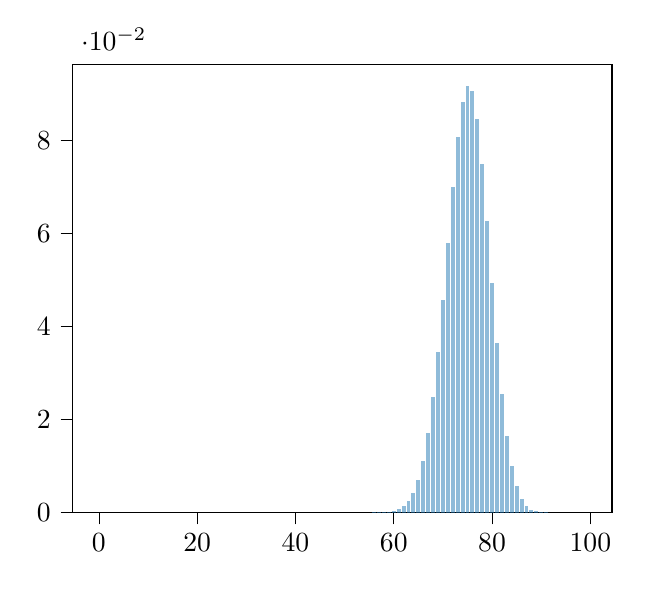
\begin{tikzpicture}

\definecolor{color0}{rgb}{0.12156862745098,0.466666666666667,0.705882352941177}

\begin{axis}[
tick align=outside,
tick pos=left,
x grid style={white!69.0196078431373!black},
xmin=-5.39, xmax=104.39,
xtick style={color=black},
y grid style={white!69.0196078431373!black},
ymin=0, ymax=0.0963896763551786,
ytick style={color=black}
]
\draw[draw=none,fill=color0,fill opacity=0.5] (axis cs:-0.4,0) rectangle (axis cs:0.4,6.22301527786114e-61);
\draw[draw=none,fill=color0,fill opacity=0.5] (axis cs:0.6,0) rectangle (axis cs:1.4,1.86690458335834e-58);
\draw[draw=none,fill=color0,fill opacity=0.5] (axis cs:1.6,0) rectangle (axis cs:2.4,2.77235330628714e-56);
\draw[draw=none,fill=color0,fill opacity=0.5] (axis cs:2.6,0) rectangle (axis cs:3.4,2.7169062401614e-54);
\draw[draw=none,fill=color0,fill opacity=0.5] (axis cs:3.6,0) rectangle (axis cs:4.4,1.97654928971742e-52);
\draw[draw=none,fill=color0,fill opacity=0.5] (axis cs:4.6,0) rectangle (axis cs:5.4,1.13849239087723e-50);
\draw[draw=none,fill=color0,fill opacity=0.5] (axis cs:5.6,0) rectangle (axis cs:6.4,5.40783885666685e-49);
\draw[draw=none,fill=color0,fill opacity=0.5] (axis cs:6.6,0) rectangle (axis cs:7.4,2.17858651082864e-47);
\draw[draw=none,fill=color0,fill opacity=0.5] (axis cs:7.6,0) rectangle (axis cs:8.4,7.5978204565149e-46);
\draw[draw=none,fill=color0,fill opacity=0.5] (axis cs:8.6,0) rectangle (axis cs:9.4,2.32999827333124e-44);
\draw[draw=none,fill=color0,fill opacity=0.5] (axis cs:9.6,0) rectangle (axis cs:10.4,6.36089528619427e-43);
\draw[draw=none,fill=color0,fill opacity=0.5] (axis cs:10.6,0) rectangle (axis cs:11.4,1.56131066115678e-41);
\draw[draw=none,fill=color0,fill opacity=0.5] (axis cs:11.6,0) rectangle (axis cs:12.4,3.47391622107383e-40);
\draw[draw=none,fill=color0,fill opacity=0.5] (axis cs:12.6,0) rectangle (axis cs:13.4,7.05472217202685e-39);
\draw[draw=none,fill=color0,fill opacity=0.5] (axis cs:13.6,0) rectangle (axis cs:14.4,1.31520177635643e-37);
\draw[draw=none,fill=color0,fill opacity=0.5] (axis cs:14.6,0) rectangle (axis cs:15.4,2.26214705533307e-36);
\draw[draw=none,fill=color0,fill opacity=0.5] (axis cs:15.6,0) rectangle (axis cs:16.4,3.60529686943707e-35);
\draw[draw=none,fill=color0,fill opacity=0.5] (axis cs:16.6,0) rectangle (axis cs:17.4,5.34432241822437e-34);
\draw[draw=none,fill=color0,fill opacity=0.5] (axis cs:17.6,0) rectangle (axis cs:18.4,7.39297934521038e-33);
\draw[draw=none,fill=color0,fill opacity=0.5] (axis cs:18.6,0) rectangle (axis cs:19.4,9.57196273116712e-32);
\draw[draw=none,fill=color0,fill opacity=0.5] (axis cs:19.6,0) rectangle (axis cs:20.4,1.1629934718368e-30);
\draw[draw=none,fill=color0,fill opacity=0.5] (axis cs:20.6,0) rectangle (axis cs:21.4,1.32913539638492e-29);
\draw[draw=none,fill=color0,fill opacity=0.5] (axis cs:21.6,0) rectangle (axis cs:22.4,1.4318413133783e-28);
\draw[draw=none,fill=color0,fill opacity=0.5] (axis cs:22.6,0) rectangle (axis cs:23.4,1.45674290143705e-27);
\draw[draw=none,fill=color0,fill opacity=0.5] (axis cs:23.6,0) rectangle (axis cs:24.4,1.40211504263316e-26);
\draw[draw=none,fill=color0,fill opacity=0.5] (axis cs:24.6,0) rectangle (axis cs:25.4,1.27872891888145e-25);
\draw[draw=none,fill=color0,fill opacity=0.5] (axis cs:25.6,0) rectangle (axis cs:26.4,1.1065923336474e-24);
\draw[draw=none,fill=color0,fill opacity=0.5] (axis cs:26.6,0) rectangle (axis cs:27.4,9.09864807665644e-24);
\draw[draw=none,fill=color0,fill opacity=0.5] (axis cs:27.6,0) rectangle (axis cs:28.4,7.11644260281343e-23);
\draw[draw=none,fill=color0,fill opacity=0.5] (axis cs:28.6,0) rectangle (axis cs:29.4,5.30052276623345e-22);
\draw[draw=none,fill=color0,fill opacity=0.5] (axis cs:29.6,0) rectangle (axis cs:30.4,3.76337116402575e-21);
\draw[draw=none,fill=color0,fill opacity=0.5] (axis cs:30.6,0) rectangle (axis cs:31.4,2.54938046595293e-20);
\draw[draw=none,fill=color0,fill opacity=0.5] (axis cs:31.6,0) rectangle (axis cs:32.4,1.6491304889133e-19);
\draw[draw=none,fill=color0,fill opacity=0.5] (axis cs:32.6,0) rectangle (axis cs:33.4,1.01946248405549e-18);
\draw[draw=none,fill=color0,fill opacity=0.5] (axis cs:33.6,0) rectangle (axis cs:34.4,6.02682233221042e-18);
\draw[draw=none,fill=color0,fill opacity=0.5] (axis cs:34.6,0) rectangle (axis cs:35.4,3.40945949079332e-17);
\draw[draw=none,fill=color0,fill opacity=0.5] (axis cs:35.6,0) rectangle (axis cs:36.4,1.84679055751305e-16);
\draw[draw=none,fill=color0,fill opacity=0.5] (axis cs:36.6,0) rectangle (axis cs:37.4,9.5833455957434e-16);
\draw[draw=none,fill=color0,fill opacity=0.5] (axis cs:37.6,0) rectangle (axis cs:38.4,4.76645346735658e-15);
\draw[draw=none,fill=color0,fill opacity=0.5] (axis cs:38.6,0) rectangle (axis cs:39.4,2.27323165366237e-14);
\draw[draw=none,fill=color0,fill opacity=0.5] (axis cs:39.6,0) rectangle (axis cs:40.4,1.04000348155053e-13);
\draw[draw=none,fill=color0,fill opacity=0.5] (axis cs:40.6,0) rectangle (axis cs:41.4,4.56586894339259e-13);
\draw[draw=none,fill=color0,fill opacity=0.5] (axis cs:41.6,0) rectangle (axis cs:42.4,1.92418762614402e-12);
\draw[draw=none,fill=color0,fill opacity=0.5] (axis cs:42.6,0) rectangle (axis cs:43.4,7.7862476034665e-12);
\draw[draw=none,fill=color0,fill opacity=0.5] (axis cs:43.6,0) rectangle (axis cs:44.4,3.02601895498357e-11);
\draw[draw=none,fill=color0,fill opacity=0.5] (axis cs:44.6,0) rectangle (axis cs:45.4,1.12971374319387e-10);
\draw[draw=none,fill=color0,fill opacity=0.5] (axis cs:45.6,0) rectangle (axis cs:46.4,4.05223407884757e-10);
\draw[draw=none,fill=color0,fill opacity=0.5] (axis cs:46.6,0) rectangle (axis cs:47.4,1.39672749100703e-09);
\draw[draw=none,fill=color0,fill opacity=0.5] (axis cs:47.6,0) rectangle (axis cs:48.4,4.6266598139608e-09);
\draw[draw=none,fill=color0,fill opacity=0.5] (axis cs:48.6,0) rectangle (axis cs:49.4,1.47297741015895e-08);
\draw[draw=none,fill=color0,fill opacity=0.5] (axis cs:49.6,0) rectangle (axis cs:50.4,4.50731087508638e-08);
\draw[draw=none,fill=color0,fill opacity=0.5] (axis cs:50.6,0) rectangle (axis cs:51.4,1.32567966914305e-07);
\draw[draw=none,fill=color0,fill opacity=0.5] (axis cs:51.6,0) rectangle (axis cs:52.4,3.74759444930825e-07);
\draw[draw=none,fill=color0,fill opacity=0.5] (axis cs:52.6,0) rectangle (axis cs:53.4,1.01821434094413e-06);
\draw[draw=none,fill=color0,fill opacity=0.5] (axis cs:53.6,0) rectangle (axis cs:54.4,2.65867077913189e-06);
\draw[draw=none,fill=color0,fill opacity=0.5] (axis cs:54.6,0) rectangle (axis cs:55.4,6.67084668218547e-06);
\draw[draw=none,fill=color0,fill opacity=0.5] (axis cs:55.6,0) rectangle (axis cs:56.4,1.60815053945542e-05);
\draw[draw=none,fill=color0,fill opacity=0.5] (axis cs:56.6,0) rectangle (axis cs:57.4,3.72413809137046e-05);
\draw[draw=none,fill=color0,fill opacity=0.5] (axis cs:57.6,0) rectangle (axis cs:58.4,8.2829967894274e-05);
\draw[draw=none,fill=color0,fill opacity=0.5] (axis cs:58.6,0) rectangle (axis cs:59.4,0.000176891117875907);
\draw[draw=none,fill=color0,fill opacity=0.5] (axis cs:59.6,0) rectangle (axis cs:60.4,0.00036262679164561);
\draw[draw=none,fill=color0,fill opacity=0.5] (axis cs:60.6,0) rectangle (axis cs:61.4,0.000713364180286445);
\draw[draw=none,fill=color0,fill opacity=0.5] (axis cs:61.6,0) rectangle (axis cs:62.4,0.00134618724344378);
\draw[draw=none,fill=color0,fill opacity=0.5] (axis cs:62.6,0) rectangle (axis cs:63.4,0.00243595786908874);
\draw[draw=none,fill=color0,fill opacity=0.5] (axis cs:63.6,0) rectangle (axis cs:64.4,0.00422486442920078);
\draw[draw=none,fill=color0,fill opacity=0.5] (axis cs:64.6,0) rectangle (axis cs:65.4,0.00701977474390283);
\draw[draw=none,fill=color0,fill opacity=0.5] (axis cs:65.6,0) rectangle (axis cs:66.4,0.011167823456209);
\draw[draw=none,fill=color0,fill opacity=0.5] (axis cs:66.6,0) rectangle (axis cs:67.4,0.0170017610825869);
\draw[draw=none,fill=color0,fill opacity=0.5] (axis cs:67.6,0) rectangle (axis cs:68.4,0.0247525639290604);
\draw[draw=none,fill=color0,fill opacity=0.5] (axis cs:68.6,0) rectangle (axis cs:69.4,0.0344383498143448);
\draw[draw=none,fill=color0,fill opacity=0.5] (axis cs:69.6,0) rectangle (axis cs:70.4,0.0457538076104867);
\draw[draw=none,fill=color0,fill opacity=0.5] (axis cs:70.6,0) rectangle (axis cs:71.4,0.0579977842949832);
\draw[draw=none,fill=color0,fill opacity=0.5] (axis cs:71.6,0) rectangle (axis cs:72.4,0.0700806560231046);
\draw[draw=none,fill=color0,fill opacity=0.5] (axis cs:72.6,0) rectangle (axis cs:73.4,0.0806407548759012);
\draw[draw=none,fill=color0,fill opacity=0.5] (axis cs:73.6,0) rectangle (axis cs:74.4,0.0882689343911892);
\draw[draw=none,fill=color0,fill opacity=0.5] (axis cs:74.6,0) rectangle (axis cs:75.4,0.0917996917668368);
\draw[draw=none,fill=color0,fill opacity=0.5] (axis cs:75.6,0) rectangle (axis cs:76.4,0.0905918010856942);
\draw[draw=none,fill=color0,fill opacity=0.5] (axis cs:76.6,0) rectangle (axis cs:77.4,0.0847092165996101);
\draw[draw=none,fill=color0,fill opacity=0.5] (axis cs:77.6,0) rectangle (axis cs:78.4,0.074935076222732);
\draw[draw=none,fill=color0,fill opacity=0.5] (axis cs:78.6,0) rectangle (axis cs:79.4,0.0626039877303837);
\draw[draw=none,fill=color0,fill opacity=0.5] (axis cs:79.6,0) rectangle (axis cs:80.4,0.0493006403376772);
\draw[draw=none,fill=color0,fill opacity=0.5] (axis cs:80.6,0) rectangle (axis cs:81.4,0.0365189928427239);
\draw[draw=none,fill=color0,fill opacity=0.5] (axis cs:81.6,0) rectangle (axis cs:82.4,0.0253851535614056);
\draw[draw=none,fill=color0,fill opacity=0.5] (axis cs:82.6,0) rectangle (axis cs:83.4,0.0165156420760952);
\draw[draw=none,fill=color0,fill opacity=0.5] (axis cs:83.6,0) rectangle (axis cs:84.4,0.0100273541176292);
\draw[draw=none,fill=color0,fill opacity=0.5] (axis cs:84.6,0) rectangle (axis cs:85.4,0.00566250585466122);
\draw[draw=none,fill=color0,fill opacity=0.5] (axis cs:85.6,0) rectangle (axis cs:86.4,0.00296293910999715);
\draw[draw=none,fill=color0,fill opacity=0.5] (axis cs:86.6,0) rectangle (axis cs:87.4,0.00143038439792966);
\draw[draw=none,fill=color0,fill opacity=0.5] (axis cs:87.6,0) rectangle (axis cs:88.4,0.000633920358173371);
\draw[draw=none,fill=color0,fill opacity=0.5] (axis cs:88.6,0) rectangle (axis cs:89.4,0.000256417223530802);
\draw[draw=none,fill=color0,fill opacity=0.5] (axis cs:89.6,0) rectangle (axis cs:90.4,9.40196486279606e-05);
\draw[draw=none,fill=color0,fill opacity=0.5] (axis cs:90.6,0) rectangle (axis cs:91.4,3.09954885586683e-05);
\draw[draw=none,fill=color0,fill opacity=0.5] (axis cs:91.6,0) rectangle (axis cs:92.4,9.09650207700049e-06);
\draw[draw=none,fill=color0,fill opacity=0.5] (axis cs:92.6,0) rectangle (axis cs:93.4,2.34748440696787e-06);
\draw[draw=none,fill=color0,fill opacity=0.5] (axis cs:93.6,0) rectangle (axis cs:94.4,5.24438005811971e-07);
\draw[draw=none,fill=color0,fill opacity=0.5] (axis cs:94.6,0) rectangle (axis cs:95.4,9.93672011012155e-08);
\draw[draw=none,fill=color0,fill opacity=0.5] (axis cs:95.6,0) rectangle (axis cs:96.4,1.55261251720649e-08);
\draw[draw=none,fill=color0,fill opacity=0.5] (axis cs:96.6,0) rectangle (axis cs:97.4,1.92075775324514e-09);
\draw[draw=none,fill=color0,fill opacity=0.5] (axis cs:97.6,0) rectangle (axis cs:98.4,1.76396120195983e-10);
\draw[draw=none,fill=color0,fill opacity=0.5] (axis cs:98.6,0) rectangle (axis cs:99.4,1.06906739512717e-11);
\end{axis}

\end{tikzpicture}

\end{center}


Au début de ce chapitre, nous avons décrit des situations probabilistes en définissant
proprement un univers $\Omega$ ainsi qu'une probabilité $\mathbb{P}$ sur $\Omega$.
Mais en avançant dans les exercices, nous nous sommes éloignés
de l'univers $\Omega$ pour décrire désormais notre expérience à l'aide de variables aléatoires.
C'est ce que nous ferons de plus en plus. La description de notre problème probabiliste
se fera par la donnée d'une ou plusieurs variables aléatoires dont nous donnerons les
lois, plutôt que de nous concentrer sur l'espace probabilisé $(\Omega,\mathbb{P})$. Cette
abstraction nous sera très utile. Par exemple, si on lance un dé à 6 faces, on a envie
de choisir $\Omega_1=\intere{1}{6}$ muni de la probabilité uniforme. Mais si on lance
deux fois le dé, l'univers $\Omega_2=\intere{1}{6}^2$ muni de la loi uniforme semble
plus approprié. Toute probabilité d'un évènement faisant intervenir les deux lancers de
dés doit être calculée dans le cadre de l'univers $\Omega_2$. Cependant $\Omega_1$ nous suffit
si on s'intéresse uniquement au premier lancer. Pour autant, doit-on changer d'univers à chaque fois
qu'on change de question~? La réponse des probabilistes à ce problème consiste à négliger
une bonne fois pour toutes l'univers $\Omega$. Par exemple, si un exercice vous met dans la
situation \og On lance un dé à 6 faces et on note $X$ la face obtenue \fg, vous pouvez
affirmer que $X$ est une variable aléatoire suivant la loi uniforme sur $\intere{1}{6}$
sans évoquer l'espace probabilisé $(\Omega,\mathbb{P})$.\\

Cependant, les mathématiciens se demandent souvent si les objets qu'ils manipulent existent bien.
En prépa, c'est un problème que nous pourrons le plus souvent ignorer. Mais, lorsque l'on souhaite
travailler avec la rigueur que nous permettent les mathématiques, il est important de démontrer que
les espaces probabilisés dont nous parlons existent bien. De nombreux théorèmes, qui ne sont pas
au programme de prépa, nous permettent de
justifier l'existence de tels espaces. Par exemple, si $E$ est un ensemble fini et $(p_x)_{x\in E}$ est
une distribution de probabilités sur $E$, on peut montrer qu'il existe bien un espace probabilisé
$(\Omega,\mathbb{P})$ et une variable aléatoire $X:\Omega\to E$ telle que
\[\forall x\in E\qsep \mathbb{P}(X=x)=p_x.\]

\section{Dépendance des évènements}

\subsection{Probabilité conditionnelle}

On se donne une expérience aléatoire associée à un espace probabilisé $(\Omega,\mathbb{P})$.
Soit $A$ et $B$ deux évènements tels que $\mathbb{P}(B)>0$. Si on réalise $n$ fois cette
expérience aléatoire et qu'on compte le nombre de fois $n_B$ où l'évènement $B$ a été réalisé
ainsi que le nombre de fois $n_{A\cap B}$ parmi ces réalisations où l'évènement $A$ a aussi
été réalisé, alors
\[\frac{n_{A\cap B}}{n_B}=\frac{n_{A\cap B}}{n}\cdot\frac{n}{n_B}
  \tendvers{n}{+\infty} \frac{\mathbb{P}(A\cap B)}{\mathbb{P}(B)}.\]
On appelle ce nombre, probabilité de $A$ sachant $B$.

\begin{definition}
Soit $B\in\mathcal{P}(\Omega)$ un évènement
de probabilité non nulle. Pour tout évènement $A\in\mathcal{P}(\Omega)$, on appelle
\emph{probabilité de $A$ sachant $B$} le nombre
\[\mathbb{P}(A|B)=\frac{\mathbb{P}(A\cap B)}{\mathbb{P}(B)}.\]
\end{definition}

\begin{proposition}
Soit $B\in\mathcal{P}(\Omega)$ un évènement
de probabilité non nulle. Alors l'application
\[\dspappli{\mathbb{P}_B}{\mathcal{P}(\Omega)}{\interf{0}{1}}{A}{\mathbb{P}(A|B)}\]
est une probabilité sur $\Omega$.
\end{proposition}

\begin{remarqueUnique}
\remarque Attention, bien qu'on écrive $\mathbb{P}(A|B)$, $A|B$ n'est pas un évènement.
  La notation $\mathbb{P}_B(A)$ protège contre cette erreur.
\end{remarqueUnique}

\subsection{Formule des probabilités totales}

\begin{proposition}[nom={Formule des probabilités totales}]
Soit $(A_1,\ldots,A_n)$ un système complet d'évènements. Alors, pour tout évènement $B$
\[\mathbb{P}(B)=\sum_{i=1}^n \mathbb{P}(A_i)\mathbb{P}(B|A_i).\]
\end{proposition}

\begin{remarques}
\remarque Dans cette formule, par convention, on remplacera
  $\mathbb{P}(A_i)\mathbb{P}(B|A_i)$ par $0$ lorsque $\mathbb{P}(A_i)=0$.
\remarque C'est cette formule qui se cache derrière les arbres de probabilité
  utilisés dans le secondaire. Afin d'aborder des exercices plus complexes,
  il est important de ne plus recourir à ces arbres et d'utiliser directement la formule
  des probabilités totales.
\end{remarques}
\vspace{1ex}
\begin{exoUnique}
\exo Une urne contient $n\in\Ns$ boules noires et $b\in\Ns$ boules blanches. On tire deux boules
  successivement sans remise. Avec quelle probabilité la deuxième boule tirée est-elle
  blanche~?
\begin{sol}
$B_1\defeq$\og La première boule tirée est blanche\fg et 
$B_2\defeq$\og La seconde boule tirée est blanche\fg. Alors $\mathbb{P}(B_1)=b/(n+b)$ et $\mathbb{P}(B_2|B_1)=(b-1)/(n+b-1)$,
$\mathbb{P}(B_2|N_1)=b/(n+b-1)$, donc $\mathbb{P}(B_2)=\frac{b}{n+b}\frac{b-1}{n+b-1}+\frac{n}{n+b}\frac{b}{n+b-1}=\frac{b}{n+b}$.
On remarque que $B_1$ et $B_2$ sont équiprobables.
\end{sol}
\end{exoUnique}

\begin{proposition}[nom={Formule des probabilités composées}]
  Soit $A_1,\ldots,A_n$ des évènements tels que $\mathbb{P}(A_1\cap\ldots\cap A_{n-1})>0$.
  Alors
  \[\mathbb{P}(A_1\cap\ldots\cap A_n)=
    \mathbb{P}(A_1)\mathbb{P}(A_2|A_1)\mathbb{P}(A_3|A_1\cap A_2)
    \cdots \mathbb{P}(A_n|A_1\cap\ldots\cap A_{n-1}).\]
\end{proposition}
  
\begin{exos}
\exo Une urne contient $2n$ boules dont $n$ noires et $n$ blanches. On en tire 3 boules successivement. Avec quelle
  probabilité les tire-t-on dans l'ordre \og noire, blanche, noire \fg si les tirages se font avec remise~? Et s'ils
  se font sans remise~?
  \begin{sol}
  Avec remise, $1/8$, sans remise $n/(4(2n-1))$.
  \end{sol}
% \exo Un commerçant met en vente 50 tickets d'un jeu dont exactement 3 sont gagnants. Je lui achète 6 tickets.
%   Avec quelle probabilité en ai-je acheté au moins un gagnant~?
\exo Une urne contient initialement une boule blanche et une boule noire. On y effectue
  $m$ tirages successifs. À chaque tirage, la boule est choisie avec une probabilité
  uniforme sur toutes les boules présentes. Avant le tirage suivant, on replace dans l’urne
  la boule tirée et on ajoute une boule supplémentaire de la même couleur. Pour tout
  $n\in\intere{1}{m}$, on désigne par $X_n$ le nombre de boules blanches obtenues au cours
  des $n$ premiers tirages.
  \begin{questions}
  \question Déterminer la loi de $X_1$, la loi de $X_2$.
  \question Calculer $\mathbb{P}(X_n = 0)$ et $\mathbb{P}(X_n = n)$.
  \question En déduire, par récurrence, la loi de $X_n$.
  \end{questions}
\begin{sol}
\begin{questions}
\question $\mathbb{P}(X_1=0)=1/2$, $\mathbb{P}(X_1=1)=1/2$. $\mathbb{P}(X_2=0)=1/3$, $\mathbb{P}(X_2=1)=$.
\end{questions}
$\mathbb{P}(X_n=k)=1/(n+1)$.
\end{sol}
\end{exos}

\subsection{Formule de \nom{Bayes}}

\begin{proposition}[nom={Formule de \nom{Bayes}}]
Soit $A$ et $B$ deux évènements de probabilité non nulle. Alors
\[\mathbb{P}(A|B)=\frac{\mathbb{P}(A)}{\mathbb{P}(B)}\cdot\mathbb{P}(B|A).\]
\end{proposition}

\begin{remarqueUnique}
\remarque Si de plus $(C_1,\ldots,C_n)$ forme un système complet d'évènements
  \[\mathbb{P}(A|B)=\frac{\mathbb{P}(A)}{%
    \sum_{i=1}^n \mathbb{P}(C_i)\mathbb{P}(B|C_i)}%
    \cdot\mathbb{P}(B|A).\]
\end{remarqueUnique}

\begin{exoUnique}
\exo Un laboratoire pharmaceutique indique pour un test permettant de détecter une maladie,
  sa sensibilité $\alpha$ qui est la probabilité que le test soit positif si le sujet est
  malade, et sa spécificité $\beta$ qui est la probabilité que le test soit négatif si le
  sujet est sain. Sachant qu'en moyenne il y a un malade sur 1000 personnes,
  calculer la probabilité pour que vous soyez un sujet sain alors que votre test est positif.
  Faites une application numérique pour $\alpha\defeq 98\%$ et $\beta\defeq 97\%$. 
   \begin{sol}
   $$\pr{S | +} = \frac{\pr{S}}{\pr{+}} \pr{+ |S}= \frac{ \frac{999}{1000}}{\pr{+}} \left( 1 - \pr{- |S} \right)= \frac{ \frac{999}{1000}}{\pr{+}} \left( 1 - \beta \right) \quad \textbf{Bayes}$$
   $$\pr{+}=\pr{+ | M} \pr{M} + \pr{+ | S} \pr{S} = \alpha \frac 1{1000} + (1-
   \beta) \frac{999}{1000} \quad \textbf{probas totales}$$
   donc $\boxed{\pr{S | +} = \frac 1{1+ \frac{\alpha}{999(1-\beta)}} \simeq
   96,8 \%}$. C'est donc très mauvais ! Si $\beta$ est très proche de $1$ alors
   $\pr{S | +}$ est proche de $0$ donc le test devient fiable \dots
   \end{sol}
\end{exoUnique}

\subsection{Indépendance}

\begin{definition}
On dit que deux évènements
$A,B\in\mathcal{P}(\Omega)$ sont \emph{indépendants} lorsque
\[\mathbb{P}(A\cap B)=\mathbb{P}(A)\mathbb{P}(B).\]
\end{definition}

\begin{remarques}
\remarque Si $A$ et $B$ sont deux évènements tels que $B$ est de probabilité non nulle,
  alors $A$ et $B$ sont indépendants si et seulement si $\mathbb{P}(A|B)=\mathbb{P}(A)$.
\remarque Il est important de ne pas confondre les notions d'incompatibilité et d'indépendance.
  Notons d'ailleurs que la notion d'incompatibilité ne dépend pas de la loi de probabilité
  utilisée alors que la notion d'indépendance en dépend.
\end{remarques}

\begin{proposition}
Soit $A$ et $B$ deux évènements indépendants. Alors $A$ et $\bar{B}$ sont indépendants.
\end{proposition}

\begin{remarqueUnique}
\remarque On en déduit que si $A$ et $B$ sont indépendants, il en est de même pour $\bar{A}$ et $B$,
 ainsi que pour $\bar{A}$ et $\bar{B}$.
\end{remarqueUnique}

\begin{definition}
On dit que les évènements
$A_1,\ldots,A_n\in\mathcal{P}(\Omega)$ sont \emph{mutuellement indépendants} lorsque,
quel que soit $I\subset\intere{1}{n}$
\[\mathbb{P}\p{\bigcap_{i\in I} A_i}=\prod_{i\in I} \mathbb{P}(A_i).\]
\end{definition}

\begin{remarques}
\remarque Si $A_1,\ldots,A_n\in\mathcal{P}(\Omega)$ sont mutuellement indépendants, alors
  ils sont deux à deux indépendants. Autrement dit
  \[\forall i,j\in\intere{1}{n}\qsep i\neq j \quad\implique\quad \mathbb{P}(A_i\cap A_j)
    =\mathbb{P}(A_i)\mathbb{P}(A_j).\]
  Cependant, comme le montre le prochain exercice, des évènements peuvent être deux à deux
  indépendants sans être mutuellement indépendants.
\remarque Si $A_1,\ldots,A_n\in\mathcal{P}(\Omega)$ sont mutuellement indépendants, alors
  $B_1\in\{A_1,\bar{A_1}\},\ldots,B_n\in\{A_n,\bar{A_n}\}$ sont mutuellement indépendants.
\end{remarques}

\begin{exoUnique}
\exo On lance successivement deux dés équilibrés. On modélise cela en prenant
  $\Omega\defeq\intere{1}{6}^2$ que l'on munit de la probabilité uniforme.
  On considère les évènements suivants~:
  \begin{itemize}
  \item $A\defeq$ \og Le premier dé est pair \fg.
  \item $B\defeq$ \og Le second dé est impair \fg.
  \item $C\defeq$ \og La somme des deux dés est paire \fg.
  \end{itemize}
  Sont-ils deux à deux indépendants~? Sont-ils mutuellement indépendants~?
  % \begin{sol}
  % Ces trois évènements sont de proba $1/2$ (pour le dernier, on peut le voir en énumérant tous les cas (dans un tableau ?)). On montre ensuite qu'ils sont deux à deux indépendants en calculant les probabilités des intersections. En revanche, $\pr{A\cap B\cap C}=0$ donc ils ne sont pas mutuellement indépendants.
  % \end{sol}
  % \exo Soit $n \geq 2$. On lance $n$ fois une pièce équilibrée. On note $A$ l'évènement \og toutes les pièces tombent du même côté \fg et $B$ l'évènement \og on obtient au plus un {\it face}\fg. $A$ et $B$ sont-ils indépendants ?
  % \begin{sol}
  % On a $\pr{A}=2\p{\frac{1}{2}}^n=\p{\frac{1}{2}}^{n-1}$ et $B$ est l'union des évènements incompatibles "on fait que des piles" et "on fait exactement un face" $\pr{B}=\p{\frac{1}{2}}^n+n\p{\frac{1}{2}}^n$. On a donc $\pr{A}\pr{B}=\frac{2(n+1)}{2^{2n}}$.
  % $A\cap B$ est l'évènement "on fait que des piles" (car $n\geq 2$) de probabilité $\pr{A\cap B}=\p{\frac{1}{2}}^n$. 
  % Les évènements $A$ et $B$ ne sont donc pas indépendants.
  % \end{sol}
\end{exoUnique}

\begin{definition}
\begin{itemize}
\item On dit que deux variables aléatoires $X:\Omega\to E$ et $Y:\Omega\to F$ sont
  \emph{indépendantes} lorsque quelles que soient les parties $A\in\mathcal{P}(E)$ et
  $B\in\mathcal{P}(F)$, les évènements $(X\in A)$ et $(Y\in B)$ sont
  indépendants.
\item On dit que $n$ variables aléatoires $X_1:\Omega\to E_1,\ldots,X_n:\Omega\to E_n$ sont
\emph{mutuellement indépendantes} lorsque quelles que soient les parties
$A_1\in\mathcal{P}(E_1),\ldots,A_n\in\mathcal{P}(E_n)$, les évènements
$(X_1\in A_1),\ldots,(X_n\in A_n)\in\mathcal{P}(\Omega)$ sont mutuellement indépendants.
\end{itemize}
\end{definition}

\begin{remarques}
\remarque Si $X$ et $Y$ sont indépendantes, on note $X \indep Y$.
\remarque Si $X_1,\ldots,X_n$ sont mutuellement indépendantes, alors elles sont
  deux à deux indépendantes. Cependant, la réciproque est fausse. Lorsqu'on parle de variables aléatoires
  indépendantes sans plus de précision, il faut comprendre que les variables aléatoires sont
  mutuellement indépendantes.
\end{remarques}

\begin{proposition}
Soit $X_1:\Omega\to E_1,\ldots,X_n:\Omega\to E_n$, $n$ variables aléatoires. Alors, elles sont mutuellement
indépendantes si et seulement si
\[\forall (x_1,\ldots,x_n)\in X_1(\Omega)\times\cdots\times X_n(\Omega)\qsep
  \mathbb{P}((X_1=x_1)\cap\cdots\cap(X_n=x_n))=\mathbb{P}(X=x_1)\cdots\mathbb{P}(X_n=x_n).\] 
\end{proposition}

\begin{remarqueUnique}
\remarque Soit $A_1,\ldots,A_n\in\mathbb{P}(\Omega)$. Alors $A_1,\ldots,A_n$ sont mutuellement
  indépendants si et seulement si les variables aléatoires $\mathds{1}_{A_1},\ldots,\mathds{1}_{A_n}$
  sont mutuellement indépendantes.
\end{remarqueUnique}

\begin{exoUnique}
\exo Soit $X,Y,Z$ trois variables aléatoires mutuellement
  indépendantes qui suivent la même loi de
  \nom{Bernoulli} de paramètre $p\in[0,1]$. Donner une condition nécessaire et
  suffisante sur $p$ pour que les évènements $(X=Y)$ et $(Y=Z)$ soient
  indépendants.
% \begin{reponse}
% On note $A=(X=Y)$ et $B=(Y=Z)$. Alors
% $$\pr{A}=\pr{\p{X=0 \cap Y=0} \cup \p{X=1 \cap Y=1}} =\pr{X=0}\pr{Y=0} + \pr{X=1} \pr{Y=1}$$
% puisque les évènements $(X=0 \cap Y=0)$ et $(X=1 \cap Y=1)$ sont incompatibles et les évènements $(X=0)$ et $(Y=0)$ sont indépendants. On a donc $\pr{A}=p^2+q^2$. De même $\pr{B}=p^2+q^2$ et $\pr{A \cap B }=p^3+q^3$. 
% Mais $(p^2+q^2)^2-(p^3+q^3)=p(p-1)(2p-1)^2$ donc \fbox{il y a indépendance ssi $p=0,1$ ou $\frac 12$}.
% \end{reponse}
\end{exoUnique}

\begin{proposition}[nom={Lemme des coalitions}]
\begin{itemize}
\item 
Soit $X_1:\Omega\to E_1,\ldots,X_n:\Omega\to E_n$, des variables aléatoires mutuellement
indépendantes et
\[f:E_1\times\cdots\times E_m\to F,\qquad g:E_{m+1}\times\cdots\times E_n\to G\]
deux fonctions. Alors, les variables aléatoires $f(X_1,\ldots,X_m):\Omega\to F$ et
$g(X_{m+1},\ldots,X_n):\Omega\to G$ sont indépendantes. 
\item Soit $A_1,\ldots,A_n$ des évènements mutuellement indépendants. Si $B$ est un
 évènement défini à partir des évènements $A_1,\ldots,A_m$ et $C$ est un évènement
 défini à partir des évènements $A_{m+1},\ldots,A_n$, alors $B$ et $C$ sont
 indépendants.
\end{itemize}
\end{proposition}

\begin{remarques}
\remarque Cet énoncé se généralise facilement à un nombre fini de coalitions et nous
  assure que les variables aléatoires et les évènements obtenus sont mutuellement
  indépendants.
\remarque Supposons que l'on lance $n$ fois une pièce et que les $n$ lancers sont
  indépendants. Si $p,q\in\N$ sont tels que $p+q=n$, alors la variable aléatoire $Y$
  donnant le nombre de pile lors des $p$ premiers lancers est indépendante de la
  variable aléatoire $Z$ donnant le nombre de pile lors des $q$ derniers lancers.
% \remarque Si $E$ et $F$ sont deux ensembles finis, $(p_x)_{x\in E}$ est une distribution
%   de probabilités sur $E$ et $(q_y)_{y\in F}$ est une distribution de probabilités sur $F$,
%   on peut montrer qu'il existe un espace probabilisé $(\Omega,\mathbb{P})$ et deux
%   variables aléatoires indépendantes $X:\Omega\to E$ et $Y:\Omega\to F$ telles que
%   \[\cro{\forall x\in E\qsep \mathbb{P}(X=x)=p_x} \quad\et\quad \cro{\forall y\in F\qsep \mathbb{P}(Y=y)=q_y}.\]
%   Bien entendu, cette proposition se généralise à un nombre fini d'ensembles finis
%   $E_1,\ldots,E_n$ et permet de justifier l'existence d'un espace probabilisé
%   $(\Omega,\mathbb{P})$ et de variables aléatoires
%   $X_1:\Omega\to E_1,\ldots,X_n:\Omega\to E_n$ mutuellement indépendantes ayant une
%   loi donnée.
\end{remarques}

\begin{exoUnique}
\exo Soit $X_1,\ldots,X_n:\Omega\to\R$ une famille de variables aléatoires mutuellement
  indépendantes suivant toutes une loi de \nom{Rademacher}. Pour tout $i\in\intere{1}{n-1}$,
  on pose $Y_i\defeq X_i X_{i+1}$.
  \begin{questions}
  \question Montrer que les variables $Y_1,\ldots,Y_{n-1}$ sont deux à deux indépendantes.
  \question Sont-elles mutuellement indépendantes~?
  \end{questions}
\end{exoUnique}



\subsection{Loi d'une somme}

\begin{proposition}
Soit $X,Y:\Omega\to\N$ deux variables aléatoires indépendantes. Alors
\[\forall n\in\N\qsep\mathbb{P}(X+Y=n)=\sum_{k=0}^n  \mathbb{P}(X=k) \mathbb{P}(Y=n-k).\]
\end{proposition}

\begin{remarqueUnique}
\remarque Plus généralement, si $X,Y:\Omega\to\N$ sont deux variables dont on
  ne fait aucune hypothèse d'indépendance
  \[\forall n\in\N\qsep \mathbb{P}(X+Y=n)=\sum_{k=0}^n  \mathbb{P}((X=k)\cap(Y=n-k)).\] 
\end{remarqueUnique}

\begin{proposition}
Soit $X,Y:\Omega\to\N$ deux variables aléatoires indépendantes. On suppose qu'il existe
$p\in[0,1]$ et $n,m\in\N$ tels que $X\sim\mathcal{B}(n,p)$ et $Y\sim\mathcal{B}(m,p)$. Alors
$X+Y\sim\mathcal{B}(n+m,p)$.
\end{proposition}

\begin{proposition}
Soit $X_1,\ldots,X_n:\Omega\to\ens{0,1}$ des variables de \nom{Bernoulli} mutuellement indépendantes de
même paramètre $p\in[0,1]$.  Alors
\[X_1+\cdots+X_n \sim \mathcal{B}(n,p).\]
\end{proposition}

\begin{exoUnique}
\exo Deux joueurs lancent une pièce de monnaie équilibrée $n$ fois chacun. Calculer la
  probabilité qu'ils obtiennent le même nombre de fois pile. En déterminer un équivalent
  lorsque $n$ tend vers $+\infty$.
\begin{sol}
Soient $X$ et $Y$ les variables aléatoires discrètes qui représentent le nombre de piles obtenus par chacun des joueurs au cours des $n$ lancers. Les variables $X$ et $Y$ sont indépendantes et suivent des loi binomiales ${\cal B}(n, 1/2)$.
\[\pr{Y=k} = \sum\limits_{k=0}^n \left( \binom{n}{k} \left( \frac 12 \right)^k
  \left( \frac 12 \right)^{n-k} \right)^2\]
\[= \frac 1{4^n} \sum\limits_{k=0}^n \binom{n}{k} ^2 = \frac 1{4^n} \binom{2n}{n}
\sim \frac{1}{\sqrt{\pi n}}\]
\end{sol}
\end{exoUnique}

%END_BOOK
\end{document}



\section{Exercices}
\setcounter{numeroexercice}{1}
\documentclass{magnolia}

\magtex{tex_driver={pdftex},
        tex_packages={xypic,nicefrac}}
\magfiche{document_nom={Exercices sur les probabilités},
          auteur_nom={François Fayard},
          auteur_mail={fayard.prof@gmail.com}}
\magexos{exos_matiere={maths},
         exos_niveau={mpsi},
         exos_chapitre_numero={25},
         exos_theme={Probabilités}}
\magmisenpage{misenpage_presentation={tikzvelvia},
              misenpage_format={a4},
              misenpage_nbcolonnes={1},
              misenpage_sol={non}}
\maglieudiff{lieu_lycee={Aux Lazaristes},
             lieu_classe={MPSI 1},
             lieu_annee={2019--2020}}
\magprocess

\begin{document}
%BEGIN_BOOK

\magsection{Espace probabilisé}
\magsubsection{Espace probabilisé}

\exercice{nom={Exercice}}
Soit $A$ et $B$ deux évènements d'un espace probabilisé $(\Omega,\mathbb{P})$. Montrer que
\[\sqrt{\mathbb{P}(A\cap B)\mathbb{P}(A\cup B)}\leq\frac{\mathbb{P}(A)+\mathbb{P}(B)}{2}\]
et étudier les cas d'égalité.
\begin{sol}
Poser $a=\mathbb{P}(A)$, $b=\mathbb{P}(B)$ et $c=\mathbb{P}(A\cap B)$. Cette inégalité revient à prouver
que $(a+b-2c)^2\geq 0$. Il y a égalité si et seulement si $a=b=c$.
\end{sol}

\exercice{nom={Exercice}}
On permute aléatoirement les lettres du mot \og \textsc{Baobab} \fg. Avec quelle probabilité
le mot obtenu est-il encore \og \textsc{Baobab} \fg~?

\exercice{nom={Exercice}}
Expliquer pourquoi, lorsqu'on lance 3 dés simultanément, on obtient plus souvent
la somme 10 que la somme 9, alors que ces deux sommes peuvent être obtenues de 6
manières chacune.

\exercice{nom={Exercice}}
On lance 4 fois de suite un dé équilibré à 6 faces. Avec quelle probabilité
obtient-on~:
\begin{questions}
\question Au moins un 6.
\question Exactement un 6.
\question Au moins 2 faces identiques.
\end{questions}

\exercice{nom={Exercice}}
Dans un lot de 20 yaourts, il y en a 3 qui ont dépassé la date de péremption. On extrait au
hasard et simultanément 4 yaourts. Quelle est la probabilité qu'un seul de ces yaourts ait
dépassé la date de péremption ?

% \begin{reponse}
% Univers = combinaisons de 4 yaourts parmi 20 puisque le tirage est simultané. $\card \p{\Omega} = \binom{20}{4}$.
% On le muni de la probabilité uniforme.
% Dénombrement des cas favorables : on doit choisir un yaourt périmé $\binom{4}{1}$ puis 3 non périmés 
% $\binom{17}{3}$ donc il y a $\binom{4}{1}\binom{17}{3}$ choix.
% La probabilité cherchée est donc $\dfrac{\binom{4}{1}\binom{17}{3}}{ \binom{20}{4}} = 
% \boxed{\frac{8}{19}}$. 
% \end{reponse}

\exercice{nom={Exercice}}
On place aléatoirement $n$ boules indiscernables dans $n$ urnes discernables. Calculer la
probabilité qu'une seule urne soit vide.
% \begin{reponse}
% Facile puisqu'une seule urne est vide ssi une est vide, toutes les autres contiennent une
% seule boule sauf une qui en contient deux. On procède par dénombrement.
% \end{reponse}

\exercice{nom={Exercice}}
On lance $n$ fois une pièce équilibrée. On appelle changement un lancer qui donne un résultat différent du précédent.
Calculer pour tout entier $k \in \intere{0}{n-1}$ la probabilité pour qu'il y ait $k$ changements.
% \begin{reponse}
% $\Omega=\{P,F\}^n$. On prend la probabilité uniforme. On dénombre. Une réalisation avec $k$ changements correspond au choix des $k$ emplacements de changement entre $2$ et $n$ puis le premier lancer (P ou F) détermine toute la suite.
% On a donc $2 \binom{n-1}{k}$ choix. $\card \Omega = 2^n$ donc la probabilité cherchée est 
% $\boxed{\frac 1{2^{n-1}} \binom{n-1}{k}}$ (la somme fait bien $1$).
% \end{reponse}

\magsubsection{Variable aléatoire}

\magsubsection{Lois usuelles}

\exercice{nom={Exercice}}
Soit $n\in\Ns$ et $X$ une variable aléatoire suivant la loi uniforme sur $\intere{1}{6n}$.
Déterminer la loi de
\[\cos\p{\frac{X\pi}{3}}.\]

\magsection{Dépendance des évènements}
\magsubsection{Probabilité conditionnelle}

\exercice{nom={Exercice}}
Un train contient $n$ places numérotées et $n$ voyageurs possèdent un billet. Le premier voyageur monte dans le train, mais il a oublié son billet et se place donc au hasard. Puis chaque personne s'installe à sa place si elle est libre et choisit une place libre au hasard sinon. Quelle est la probabilité que la dernière personne se trouve à sa place ?
% \begin{reponse}
% On note $P_i=j$ l'évènement "la personne $i$ est à la place $j$" et $p_n=\pr{P_n=n}$.
% On conditionne suivant la place qu'occupe $P_1$.
% $$p_n=\pr{P_n=n}=\sum\limits_{k=1}^n \prc{P_n=n}{P_1=k} \underbrace{\pr{P_1=k}}_{=\frac 1n}
% =\frac 1n \sum\limits_{k=1}^{n-1} \prc{P_n=n}{P_1=k} $$
% Mais si $P_1=k$ alors tous les voyageurs jusqu'au $k-1$-ième inclus vont à leur place puis arrive le $k$-ième qui trouve sa place occupée et doit donc choisir au hasard une place. On se retrouve donc dans la même situation qu'au début mais il reste $n-k+1$ voyageurs. On a donc 
% $$\boxed{p_n=\frac 1n \sum\limits_{k=1}^{n-1} p_{n-k+1} =\frac 1n \sum\limits_{k=1}^{n-1} p_{k} }$$
% avec $p_1=1$, $p_2=\frac 12$ on obtient par récurrence, $\boxed{p_n=\frac 12}$.
% \end{reponse}



% \begin{reponse}
% \begin{enumerate}
% \item La plante donne une fleur rose toutes les années ssi elle donne une fleur rose la première année donc la probabilité vaut $\boxed{\frac 34}$.
% \item La plante donne une fleur blanche la première année est probabilité $\frac 14$ puis chaque année avec probabilité $\frac 12$ donc par indépendance, la probabilité cherchée est $\boxed{\frac 14 \p{\frac 12}^{n-1}}$.
% \item On $R_n$ l'évènement : la plante a donné une fleur rose l'année $n$ et $B_n$ pour blanche. On a alors
% $$\pr{R_{n+1}}=\prc{R_{n+1}}{R_n} \pr{R_n}+ \prc{R_{n+1}}{B_n} \pr{B_n}$$
% $$p_{n+1}=p_n+ \frac 12 (1-p_n)$$
% $$\boxed{p_{n+1}=\frac 12 p_n + \frac 12}$$
% Si on pose $x_{n}=p_n-1$ alors $x_{n+1}=\frac 12 x_n$ et comme $x_1=- \frac 14$ on a $x_n=-\frac 14 \p{\frac 12}^{n-1}$ et finalement
% $$\boxed{p_n = 1 -\frac 14 \p{\frac 12}^{n-1}}$$
% En particulier, $p_n \to 1$ donc à coup presque sûr la fleur deviendra définitivement rose.
% \end{enumerate}
% \end{reponse}

\exercice{nom={Exercice}}
$n$ personnes numérotées de $1$ à $n$ se transmettent dans cet ordre une
information binaire.
Chaque personne transforme l'information reçue en son contraire
avec la probabilité $p \in ]0,1[$ et la transmet fidèlement avec la probabilité
$1-p$. Quelle est la probabilité que l'information correcte parvienne à la $n$-ième
personne ?

% \begin{reponse}
% On note $A_n$ l'évènement "la $n$-ième personne reçoit l'information non
% déformée" et $p_n=\pr{A_n}$.
% Pour $n \in \{1,\dots,N-1\}$, $\{ A_n, \co{A_n} \}$ est un système complet
% d'évènements donc d'après la \textbf{formule des probabilités totales}
% $$\pr{A_{n+1}}=\pr{A_n} \pr{A_{n+1} | A_n} + \pr{\co{A_n}} \pr{A_{n+1} | \co{A_n}}$$
% $$p_{n+1}=p_n (1-p) + (1-p_n) p =(1-2p) p_n + p$$
% On pose $p_1=1$ et on a une suite arithmético-géométrique ce qui donne
% $$\boxed{p_N = \frac 12 \left( 1+ (1-2p)^{N-1} \right)}$$
% En particulier, $p_N \to \frac 12$ et ceci indépendamment de la valeur de
% $p$ !
% \end{reponse}

\exercice{nom={Exercice}}%vincent
On dispose de $n+1$ urnes $U_0, U_1, \dots, U_n$ où l'urne $U_k$
contient $k$ boules blanches et $n-k$ boules noires. On choisit une
urne au hasard puis on réalise $p$ tirages avec remise dans l'urne
choisie.
\begin{questions}
\question Quelle est la probabilité de ne tirer que des boules blanches ?
\question Déterminer la limite de cette probabilité lorsque $n$ tend vers $+\infty$.
\end{questions}

% \begin{reponse}
% \begin{enumerate}
% \item
% On note $U_k$ l'évènement : "on a choisi l'urne $U_k$" et $B_p$ l'évènement : "on a tiré $p$ boules blanches".
% Comme le tirage de l'urne est uniforme, $\pr{U_k} = \frac 1{n+1}$.
% \medskip
% La famille $(U_0, \dots, U_n)$ est un système complet d'évènements donc la formule des probabilités totales donne
% $$\pr{B_p} = \sum\limits_{k=0}^n \prc{B_p}{U_k} \pr{U_k} = \frac 1{n+1} \sum\limits_{k=0}^n \prc{B_p}{U_k}$$
% On note $BL_i$ l'évènement : "on a tiré une boule blanche au $i$-ième tirage". On a donc 
% $$\prc{B_p}{U_k} = \prc{BL_1 \cap \dots \cap BL_p}{U_k} = \prc{BL_1}{U_k} \dots \prc{BL_p}{U_k} = 
% \prc{BL_1}{U_k}^p$$
% par indépendance des tirages successifs et par le fait qu'ils sont avec remise. Il reste donc
% $$\prc{B_p}{U_k} = \p{\frac kn}^p \text{ donc } \boxed{\pr{B_p} = \frac 1{n+1} \sum\limits_{k=0}^n \p{\frac kn}^p}$$
% \item On utilise une somme de Riemann ou une comparaison somme-intégrale pour obtenir
% $$\boxed{ \pr{B_p} \to \frac 1{p+1} \text{ quand } n \to + \infty}$$
% \end{enumerate}
% \end{reponse}





\exercice{nom={Exercice}}%\textbf{[pêche à la grenouille]}
Soit ${\cal G}$ un ensemble fixé de cardinal $N$ et ${\cal M}$ une partie fixée de ${\cal G}$ de cardinal $m$. L'ensemble des parties de ${\cal G}$ est muni de la probabilité uniforme. On fixe $n \leq N$.
\begin{enumerate}
\item Soit $k \in \intere{0}{\min(n, m)}$. Quelle est la probabilité $p_k$ qu'une partie ${\cal P}$ de ${\cal G}$ de cardinal $n$ intersecte ${\cal M}$ selon un ensemble de cardinal $k$~?
\item Le cardinal moyen de l'intersection d'une partie ${\cal P}$ de ${\cal G}$ de cardinal $n$ avec ${\cal M}$ est donc \[\sum\limits_{k=0}^{\min(n,m)} k p_k.\] Calculer ce nombre moyen.
\item Un étang contient $N$ grenouilles. On cherche à estimer $N$. Pour cela, on commence par pêcher $m$ grenouilles que l'on marque puis que l'on rejette à l'eau. Quelques jours plus tard, on pêche $n$ grenouilles. Montrer que l'on peut estimer $N$.
\end{enumerate}

\exercice{nom={Exercice}}
On considère une urne contenant $n$ boules numérotées. Les nombres inscrits sur les boules sont des réels deux à deux distincts sur lesquels on ne sait rien de plus.
On réalise un tirage sans remise dans l'urne avec l'objectif de déterminer le maximum $M$ des nombres inscrits sur les boules.
Comme on n'a pas le temps de tirer toutes les boules (disons que $n$ est trop grand), on opte pour la stratégie suivante : on choisit un entier $p \in \intere{1}{n-1}$, on tire $p$ boules successivement et sans remise et on mémorise le maximum $M_p$ que l'on a vu parmi ces $p$ boules. On continue alors à tirer des boules, mais on s'arrête dès que l'on a trouvé un nombre supérieur à $M_p$. 
\begin{enumerate}
\item Quelle est la probabilité $P_{n,p}$ que l'on trouve ainsi le maximum $M$.
\item Si $n=4$, quelle valeur de $p$ a-t-on intérêt à choisir ?
\item Soit $\alpha \in ]0,1]$. On choisit $p$ en fonction de $n$ (on le notera donc $p_n$) de manière à ce que 
\[\frac{p_n}{n} \tendvers{n}{+\infty} \alpha.\] ($\alpha$ représente donc asymptotiquement la proportion de boules que l'on commence par tirer).
Montrer que $P_{n,p_n}$ tend vers $-\alpha \ln(\alpha)$ lorsque $n \to + \infty$.
\item Quelle valeur de $\alpha$ a-t-on intérêt à choisir ?
\end{enumerate}



% \begin{sol}
% \begin{enumerate}
% \item 
% On note $A_k$ l'évènement "le maximum $M$ se trouve en position $k$ dans le tirage". On a par équiprobabilité 
% $\pr{A_k}=\frac 1n$. 
% On note $G$ l'évènement "on gagne i.e. on a trouvé le maximum".
% On a évidemment $\prc{G}{A_k}=0$ si $k \leq p$ puisqu'alors le maximum fait partie de l'échantillon des $p$ premières boules et l'on ne trouvera plus le maximum parmi les boules qui restent.
% Ainsi, puisque $(A_1,\dots,A_n)$ est un système complet, la formule des probabilités totales donne
% $$\pr{G} = \sum\limits_{k=p+1}^n \prc{G}{A_k} \pr{A_k} = \frac 1n \sum\limits_{k=p+1}^n \prc{G}{A_k}$$
% Il reste donc à calculer $\prc{G}{A_k}$. Mais, si $M$ est en position $k$, on gagne ssi entre les boules $p+1$ et $k-1$ on a trouvé aucune valeur supérieure à $M_p$ ssi le max des valeurs des boules de $1$ à $k-1$ est obtenu parmi les $p$ premières boules et ceci est réalisé avec une probabilité $\frac{p}{k-1}$ (équiprobabilité). On a donc
% $$\boxed{P_{n,p}} = \frac 1n \sum\limits_{k=p+1}^n \frac{p}{k-1} = \boxed{ \frac pn \sum\limits_{k=p}^{n-1} \frac{1}{k} }$$
% \item 
% La formule précédente montrer que 
% $$P_{4,1}=\frac{11}{24} \qquad P_{4,2}=\frac{10}{24} \qquad P_{4,3}=\frac{6}{24}$$
% de sorte que l'on a intérêt à choisir $\boxed{p=1}$.
% \item On utilise le développement asymptotique bien connu de $H_n=\sum\limits_{k=1}^n \frac 1k = 
% \ln(n) + \gamma + o(1)$ ce qui donne facilement le résultat.
% \item On maximise facilement la fonction $\alpha \mapsto - \alpha \ln(\alpha)$ ce qui donne que le maximum est atteint en 
% $\frac 1e$ et vaut $\frac 1e$. On a donc intérêt à prendre $\boxed{p \sim \frac 1e n}$.
% \end{enumerate}
% \end{sol}


%\exercice{nom={Exercice}}On dispose d'une pièce truquée pour laquelle la probabilité de faire {\it pile} est $p$. On ne connait pas $p$. Pour l'estimer, on lance la pièce 10 fois et on obtient $3$ fois {\it pile}. Quelle est la valeur de $p$ rendant cet évènement le plus probable ?
%


%\exercice{nom={Exercice}}
%On transmet un message en binaire sous forme d'une suite de $n$ bits.
%Lors de la transmission, chaque bit a une probabilité $p$ d'être modifié. Quelle est la probabilité que le message reçu comporte au plus une erreur ?
%
%\begin{reponse}
%Le nombre de bits erronés suit une loi binomiale de paramètres $n,q$.
%
%La probabilité cherchée est donc $\boxed{q^n+npq^{n-1}}$.
%\end{reponse}
%



%
%\exercice{nom={Exercice}}
%On considère un gène possédant deux caractères $a$ et $A$. Le génotype d'un individu est donc $aa$, $aA$ ou $AA$.
%On suppose qu'à la génération $0$, les proportions de porteurs $aa$, $aA$ et $AA$ sont respectivement $u_1,u_2$ et $u_3$.
%
%On fait l'hypothèse que les mariages sont aléatoires et la transmission des caractères uniforme.
%
%On note $M$ le génotype de la mère, $P$ celui du père et $E$ celui de l'enfant. On note $x=u_1+ \frac 12 u_2$. Montrer qu'à la génération 1,
%$$\pr{ E = \text{aa} } = x^2 \qquad \pr{ E = \text{aA} } = 2x(1-x) \qquad \pr{ E = \text{AA} } = (1-x)^2 \qquad$$
%En déduire que les proportions sont constantes à partir de la première génération.
%
%

\magsubsection{Formule des probabilités totales}

\exercice{nom={Monthy Hall}}
Dans une fête foraine, on vous propose le jeu suivant~: trois verres opaques sont
retournés devant vous, dont l'un seulement abrite une bille, et vous devez deviner lequel.
\begin{questions}
\question Quelle est la probabilité de deviner juste~?
\question Pris de pitié devant votre malchance à répétition, le maître du jeu décide 
  de vous donner un coup de pouce. Après votre réponse, il vous indique, parmi les deux
  verres que vous n'avez pas désignés, une verre qui ne contient pas la bille et vous
  propose de revoir votre réponse. Préférez-vous confirmer votre réponse initiale ou
  la modifier~?
\end{questions}

\exercice{nom={Exercice}}
Un horticulteur dispose d'un stock de plantes. Chacune des plantes fleurit une fois par an.
Pour chaque plante, la première année, la probabilité de donner une fleur rose est de \nicefrac{3}{4},
celle de donner une fleur blanche est de \nicefrac{1}{4}.  Puis les années suivantes, pour tout entier naturel $n$ non nul :
\begin{itemize}
\item Si l'année $n$, la plante a donné une fleur rose, alors l'année $n+1$, elle donnera
  une fleur rose.
\item Si l'année $n$, la plante a donné une fleur blanche, alors l'année $n+1$, elle
  donnera de façon équiprobable une fleur rose ou une fleur blanche.
\end{itemize}
\begin{enumerate}
\item Quelle est la probabilité que la plante ne donne que des fleurs roses pendant les $n$
premières années ?
\item Quelle est la probabilité que la plante ne donne que des fleurs blanches pendant les $n$
premières années ?
\item On note $p_n$ la probabilité de l'évènement \og
  La plante a donné une fleur rose l'année $n$ \fg.
Calculer $p_n$, puis sa limite quand $n$ tend vers $+\infty$.
\end{enumerate}


\exercice{nom={Urnes d'\nom{Ehrenfest}}}%\textbf{[urnes d'Ehrenfest = chaîne de Markov]}
On considère deux urnes $U_1$ et $U_2$. Chaque urne contient une boule. À chaque étape, on choisit une boule au hasard et on la change d'urne. Pour tout $k \in \{0,1,2\}$ et
$n\in\N$, on note $E_n^k$ l'évènement \og Il y a $k$ boules dans l'urne $U_1$ après
l'étape $n$ \fg. On note
\[a_n \defeq \mathbb{P}\p{E_n^0},\quad b_n \defeq \mathbb{P}\p{E_n^1}, \quad
  c_n \defeq \mathbb{P}\p{E_n^2}, \et 
  X_n \defeq \trans{(a_n, b_n, c_n)}.\]
\begin{questions}
\question Déterminer une matrice $A\in\mat{3}{\R}$ telle que pour tout $n\in\N$,
$X_{n+1}=A X_n$.
\question Calculer $A^2$ et $A^3$.
\question Comment interpréter ce résultat~?
\end{questions}
% \begin{reponse}
% On trouve $A=\begin{pmatrix} 0 & \frac 12 & 0 \\ 1 & 0 & 1 \\ 0 & \frac 12 & 0 \end{pmatrix}$ puis $A^3=A$.
% \end{reponse}

\exercice{nom={Jinko}}
\nom{Jinko} le chaton a trois passions dans la vie~: Manger, Dormir et Jouer. On peut
  considérer qu'il pratique ces activités par tranches de 5 minutes.
  \begin{itemize}
  \item Après 5 minutes de repas, il continue de manger les 5 minutes suivantes avec une
    probabilité de \nicefrac{1}{2}. Sinon, il se met à jouer.
  \item Après 5 minutes de sommeil, il continue de dormir les 5 minutes suivantes avec une
    probabilité de \nicefrac{3}{4}. Sinon, il a faim au réveil et va manger.
  \item Après 5 minutes de jeu, soit il est en appétit et mange les 5 minutes suivantes
    avec une probabilité de \nicefrac{1}{4}, soit il est fatigué et s'endort.
  \end{itemize}
  L'expérience que l'on considère est une journée de \nom{Jinko} de $5(m+1)$ minutes. Sur la
  tranche d'indice 0 des 5 premières minutes de la journée, \nom{Jinko} se lève et va
  petit-déjeuner. Pour tout $n\in\intere{0}{m}$, on note $A_n:\Omega\to\ens{M,D,J}$ la
  variable aléatoire donnant l'activité de \nom{Jinko} sur la tranche de 5 minutes
  d'indice $n$ de la journée. Pour tout
  $n\in\intere{0}{m}$, on pose
  \[X_n\defeq
    \begin{pmatrix}
    \mathbb{P}(A_n=M)\\
    \mathbb{P}(A_n=D)\\
    \mathbb{P}(A_n=J)
    \end{pmatrix}.\]
  \begin{questions}
  \question Déterminer une matrice $B\in\mat{3}{\R}$ telle que
    \[\forall n\in\intere{0}{m-1}\qsep X_{n+1}=B X_n.\]
  \question
    \begin{questions}
    \question Déterminer les valeurs propres de $B$, c'est-à-dire les $\lambda\in\R$ tels
      que $B-\lambda I_3$ n'est pas inversible.
    \enonce On note $\lambda_1,\lambda_2,\lambda_3\in\R$ ces valeurs et on pose
      $P\defeq(X-\lambda_1)(X-\lambda_2)(X-\lambda_3)$.
    \question Montrer que $P(B)=0$. En déduire une expression de $B^n$ valable pour tout
      $n\in\N$.
    \question En déduire les limites de
      \[\mathbb{P}(A_n=M),\qquad
        \mathbb{P}(A_n=D),\qquad
        \mathbb{P}(A_n=J)\]
      lorsque $n$ tend vers $+\infty$.
    \end{questions}
  \end{questions}

\magsubsection{Formule de \nom{Bayes}}

\exercice{nom={Exercice}}
On prend un dé au hasard parmi un lot de 100 dés dont on sait que 25
sont pipés~: pour ces dés, la probabilité d'obtenir $6$ est $1/2$.
\begin{questions}
\question On lance le dé et on obtient $6$.
  Quelle est la probabilité que ce dé soit pipé~?
\question Même question si l'on fait $n$ lancers et que l'on obtient
  $6$ à chaque fois.
\end{questions}
% \begin{reponse}
% On note $DP$ l'évènement "le dé est pipé" et $A_1$ l'évènement "on obtient
% $6$ au premier lancers".
% On a alors par la \textbf{formule de Bayes} :
% \begin{eqnarray*}
% \pr{DP | A_1 }& = &\frac{\pr{DP} \pr{A_1 | DP}}{\pr{DP} \pr{A_1 | DP} +
% \pr{\co{DP}} \pr{A_1 | \co{DP}}} \\
% & = &\frac{ \frac 14 \pr{A_1 | DP}}{  \frac 14 \pr{A_1 | DP} + 
% \frac 34 \pr{A_1 | \co{DP}}}=\frac{ \frac 14  \frac 12 }{  \frac 14 \frac 12  +
%  \frac 34  \frac 16} =\frac 12 \\
% \end{eqnarray*}
% De la même manière en notant $A_n$ l'évènement "on obtient $6$ aux $n$ lancers"
% :
% \begin{eqnarray*}
% \pr{DP | A_n }& = &\frac{\pr{DP} \pr{A_n | DP}}{\pr{DP} \pr{A_n | DP} + \pr{\co{DP}}
% \pr{A_n | \co{DP}}} \\
% & = &\frac{ \frac 14 \pr{A_n | DP}}{  \frac 14 \pr{A_n | DP} + 
% \frac 34 \pr{A_n | \co{DP}}}=\frac{ \frac 14  \frac{1}{2^n} }{  \frac 14 \frac{1}{2^n}  + %
% \frac 34  \frac{1}{6^n}} =\frac {1}{1+ \frac{1}{3^{n-1}}} \\
% \end{eqnarray*}
% On a donc $\pr{DP | A_n } \to 1$ ce qui est raisonnable\dots
% \end{reponse}

\magsubsection{Indépendance}



\exercice{nom={Exercice}}
Un concours consiste à passer 3 épreuves indépendantes. On a $80 \%$ de chances de réussir
l'épreuve $1$, $60\%$ pour l'épreuve $2$ et $25\%$ pour l'épreuve $3$. On est reçu au
concours si on réussit au moins deux épreuves sur trois (n'importe lesquelles). Quelle est
la probabilité de réussir le concours ?

% \begin{reponse}
% On note $R_k$ l'évènement "on a réussi l'épreuve $k$" et $R$ l'évènement
% "on a réussi le concours". Alors
% $$R = \left( R_1 \cap R_2 \cap \co{R_3} \right) \cup \left( R_2 \cap R_3 \cap \co{R_1} \right) \cup \left( R_1 \cap R_3 \cap \co{R_2} \right) \cup
% \left( R_1 \cap R_2 \cap R_3 \right)$$
% et c'est une partition donc en passant aux probabilités (par exemple, $R_1$
% et $R_2$ sont indépendants) on obtient
% $$\pr{R} = \pr{R_1} \pr{R_2} \left( 1 - \pr{R_3} \right) + \dots = \boxed{59
% \%}$$
% \end{reponse}

\exercice{nom={Exercice}}
On dispose d'un dé à quatre faces non pipé. On réalise $n$ lancers indépendants.
On note $T$ l'évènement  \og Lors des $n$ lancers, les quatre numéros sont sortis \fg.
En utilisant la formule du crible, calculer la probabilité de $T$, puis sa limite lorsque $n$
tend vers $+\infty$.
% \begin{reponse}
% On note $A_k$ l'évènement "lors des $n$ lancers, le numéro $k$ n'est jamais sorti". Alors 
% $$\co{T} = A_1 \cup A_2 \cup A_3 \cup A_4$$
% En utilisant la formule du crible, on a donc
% $$1- \pr{T} = \pr{A_1} + \dots + \pr{A_4} - \pr{A_1 \cap A_2} - \dots - \pr{A_3 \cap A_4} 
% + \pr{A_1 \cap A_2 \cap A_3} + \dots - \pr{A_1 \cap \dots \cap A_4}$$
% ce qui donne facilement
% $$\pr{T} = 1 - 4 \p{\frac 34}^n + 6 \p{\frac 12}^n - 4 \p{\frac 14}^n \to 1$$
% ce qui est bien naturel \dots
% \end{reponse}

\exercice{nom={Formule du crible}}
On lance un dé équilibré à 6 faces $n$ fois de suite.
\begin{questions}
\question Calculer la probabilité de l'événement \og La face $i$ n'apparait jamais \fg
  pour tout $i\in\intere{1}{6}$.
\question Calculer la probabilité de l'événement \og Chacune des faces 1, 2 et 3 apparait au moins une fois \fg.
\end{questions}

\exercice{nom={Secret santa}}
Les $n$ convives ont tous posé un cadeau près du grand sapin. À minuit, on distribue au
hasard un cadeau à chaque convive, éventuellement celui qu'il a apporté.
\begin{questions}
\question À combien estimez-vous la probabilité de l'événement $E_n$ \og Personne n'a
reçu son propre cadeau \fg lorsque $n$ est grand~?
\enonce On appelle \emph{dérangement} de $\intere{1}{n}$ toute permutation sans
point fixe de $\intere{1}{n}$. On notera $D_n$ l'ensemble des dérangements de
$\intere{1}{n}$ et pour tout $k\in\intere{1}{n}$, $F_k$ l'ensemble des permutations de
$\intere{1}{n}$ qui fixent $k$.
\question Montrer que
\[\abs{D_n}=n! \sum_{k=0}^n \frac{(-1)^k}{k!}.\]
\question Calculer la probabilité de l'événement $E_n$ de la première question, puis sa
limite lorsque $n$ tend vers $+\infty$. On rappelle que pour tout $x\in\R$
\[\sum_{k=0}^n \frac{x^k}{k!}\tendvers{n}{+\infty}\e^x.\]
\end{questions}

\magsubsection{Loi d'une somme}


\exercice{nom={Centre d'appels}}
 Dans un centre d'appels, un employé effectue successivement $n$ appels
  téléphoniques vers $n$ correspondants distincts dont chacun décroche avec une
  probabilité $p\in\interf{0}{1}$.
  \begin{questions}
  \question Déterminer la loi du nombre $N_1$ de correspondants qui ont décroché.
  \question L'employé rappelle plus tard les $n-N_1$ correspondants qui n'ont pas décroché
    lors de la première série d'appels. On note $N_2$ le nombre de correspondants
    qui ont décroché cette fois. Enfin, on pose $N\defeq N_1+N_2$. Cette variable aléatoire donne
    le nombre total de personnes qui ont été contactées avec succès.
    \begin{questions}
    \question Pour tout $k,i\in\intere{0}{n}$, calculer $\mathbb{P}(N=k|N_1=i)$.
    \question En déduire la loi suivie par $N$.
    \end{questions}
    % Quelle est la loi du nombre total $N\defeq N_1+N_2$
    % de correspondants qui ont décroché~?
  \end{questions}
  \begin{sol}
Il faut calculer $\mathbb{P}(N=k)=\sum \mathbb{P}(N_1=i) \mathbb{P}(n=k|N_1=i)$. On utilise une relation sur
les coefficients binomiaux qui se montre facilement en passant par les factorielles. On trouve que $N$ suit une
loi binomiale de paramètre $n,p(2-p)$.
  \end{sol}



%END_BOOK
\end{document}


















\end{document}
